\section{GENERAL CORE-DESCRIPTION MODULES}\label{sect:modesc1}

\subsection{The \moc{RESINI:} module}\label{sect:resini}

\vskip 0.2cm
The \moc{RESINI:} module is used for modeling of the reactor fuel
lattice in \dusa{3-D} Cartesian geometry or \dusa{3-D} Hexagonal geometry. 
This modeling is based on the following considerations:

\begin{itemize}

\item For \dusa{3-D} Cartesian geometry, the reactor fuel lattice is composed of 
a well defined number of fuel channels. Each channel is composed of a well defined 
number of {\sl fuel bundles}. In \moc{RESINI:} terminology, a {\sl fuel bundle}
can be a CANDU fuel cluster or an axial slice of a PWR or FBR assembly with
homogeneous cross sections. Each reactor channel is identified by its specific name
which corresponds to its position in the fuel lattice.

\vskip 0.08cm

In a Candu reactor, the channels are refuelled according
to the bidirectional refuelling scheme. The refuelling scheme of a channel
corresponds to the number of displaced fuel bundles (bundle-shift) during
each channel refuelling. The direction of refuelling corresponds to the
direction of coolant flow along the channel. 

\vskip 0.08cm

In a PWR, a basic assembly layout can be projected over the fuel map using a
naval-coordinate position system. Assembly refuelling and shuffling will be possible using
the ad hoc module {\tt SIM:} (see \Sect{sim}).

\item For \dusa{3-D} Hexagonal geometry, the reactor fuel lattice is composed of
a well defined number of fuel channels and each channel is composed of a well defined
number of fuel bundle. All fuel bundles have the same volume. All channels contain
the same number of fuel bundles. Refuelling is not available during the calculation. The
lattice indexation is kept to identify the hexagons.

\item The fuel regions generally have a different set of global and local
parameters. For example, the fuel bundles have a different evolution of the
fuel properties according to the given burnup distribution, which is a global
parameter. Consequently, the homogenized cell properties will differ from one
fuel region to another, i.e., they are not uniform over the fuel lattice. Thus,
the realistic modeling of a reactor core requires the fuel properties to be
interpolated with respect to global and local parameters, which must be
specified in the fuel map.

\end{itemize}

\noindent
Note that the above considerations correspond to the typical core modeling
of CANDU or PWR reactors. The \moc{RESINI:} module will create a new \moc{FMAP}
object that will store the information related to the fuel lattice specification and
properties (see \Sect{resinidat}).

\noindent
In PWR cases, each channel correspond to an assembly. Using heterogeneous mixtures in one assembly increases the complexity of the geometry. However, two levels geometries (embedded geometry) are not possible in the DONJON code. The general idea is then to define one channel per mixture for all assemblies. All these channels have then to be regrouped by assembly to impose the same burnup. This process could be done manually, but if the heterogeneity of the cross-section is large (ex. one mixture per pin within a complete core), the geometry definition may be too complex. This task can be performed automatically by the module {\tt NAP:}. 

\noindent
The \moc{RESINI:} module specifications are:

\begin{DataStructure}{Structure \moc{RESINI:}}
$\{$ \dusa{FLMAP} \dusa{MATEX} \moc{:=}
\moc{RESINI:} \dusa{MATEX} $[$\dusa{COMPO}$]$ \moc{::} \dstr{descresini1} $|$ \\
~~~\dusa{FLMAP} \moc{:=} \moc{RESINI:} \dusa{FLMAP} $[$\dusa{FLMAP2}$]$
\moc{::} \dstr{descresini2} $\}$\\
\end{DataStructure}

\noindent where
\begin{ListeDeDescription}{mmmmmmmm}

\item[\dusa{FLMAP}] \texttt{character*12} name of the \dds{resini} object
that will contain the fuel-lattice information. If \dusa{FLMAP} appears on
both LHS and RHS, it will be updated; otherwise, it is created.

\item[\dusa{MATEX}] \texttt{character*12} name of the \dds{matex} object
specified in the modification mode. \dusa{MATEX} is required
only when \dusa{FLMAP} is created.

\item[\dusa{COMPO}] {\tt character*12} name of the \dds{multicompo} data
structure ({\tt L\_COMPO} signature) where the detailed subregion geometry at assembly level is stored.

\item[\dusa{FLMAP2}] \texttt{character*12} name of the \dds{resini} object
that contains the fuel-lattice information to recover from.

\item[\dstr{descresini1}] structure describing the main input data to
the \moc{RESINI:} module. Note that this input data is mandatory and
must be specified only when \dusa{FLMAP} is created.

\item[\dstr{descresini2}] structure describing the input data for global
and local parameters. This data is permitted to be modified in the
subsequent calls to the \moc{RESINI:} module.

\end{ListeDeDescription}

\vskip 0.2cm
\subsubsection{Main input data to the \moc{RESINI:} module}\label{sect:resinimain}

\noindent
Note that the input order must be respected.\\

\begin{DataStructure}{Structure \dstr{descresini1}}\label{table:descresini1}
$[$ \moc{EDIT} \dusa{iprint} $]$\\
%~\moc{NCHAN} \dusa{nch}\\
%~\moc{NBUND} \dusa{nb}\\
~\moc{:::}  $[$ \moc{SPLIT-NAP:} $]$ \moc{GEO:} \dstr{descgeo} \\
~$[$ \moc{:::}  \moc{NAP:} \dstr{descnap3} $]$ \\
~$[$ \moc{ASSEMBLY}  \dusa{na} \dusa{nax} \dusa{nay}  \\
~~ \moc{A-ZONE} $\{$ (\dusa{iza}(i) ,  i = 1, \dusa{nch}) \moc{A-NX} (\dusa{nbax}(i) ,  i = 1, \dusa{nay}) \moc{A-IBX} (\dusa{ibax}(i) ,  i = 1, \dusa{nay}) $|$ \moc{ASBLY} $\}$ \\
~~ \moc{AXNAME} (\dusa{XNAMEA}(i) ,  i = 1, \dusa{nax}) \\
~~ \moc{AYNAME} (\dusa{YNAMEA}(i) ,  i = 1, \dusa{nay}) $]$ \\
~$\{$ \moc{NXNAME}  (\dusa{XNAME}(i) ,  i = 1, \dusa{nx}) \moc{NYNAME} (\dusa{YNAME}(i) ,  i = 1, \dusa{ny}) \\
~~~~~~~~~~~~~$|$ \moc{NHNAME} (\dusa{HNAME}(i) ,  i = 1, \dusa{nh}) $\}$ \\
~$[$ \moc{SIM} \dusa{lx} \dusa{ly} (\dusa{naval}(i) ,  i = 1, \dusa{nch}) $]$ \\
~$[$ \moc{FOLLOW} \dusa{nis} (\dusa{HISOT}(i) ,  i = 1, \dusa{nis}) $]$ \\
~\moc{NCOMB} $\{$ \dusa{ncomb} ~\moc{B-ZONE}
(\dusa{icz}(i) ,  i = 1, \dusa{nch}) $|$ \moc{ALL} $|$ \moc{ASBLY} $\}$ \\
~\dstr{descresini2}\\
\end{DataStructure}

\noindent where
\begin{ListeDeDescription}{mmmmmmmm}

\item[\moc{EDIT}] keyword used to set \dusa{iprint}.

\item[\dusa{iprint}] integer index used to control the printing on screen:
 = 0 for no print; = 1 for minimum printing (default value); larger values
produce increasing amounts of output.

\item[\moc{:::}] keyword used to indicate the call to an embedded module.

\item[\moc{SPLIT-NAP:}] keyword to specify that the embedded geometry will be split by the embedded \moc{NAP:} module .

\item[\moc{GEO:}] keyword used to call the \moc{GEO:} module.
The fuel-map geometry differs from the complete reactor geometry
in the sense that it must be defined as a coarse geometry, i.e. without
mesh-splitting over the fuel bundles. Consequently, the mesh-spacings
over the fuel regions must correspond to the bundle dimensions (e.g.
$h_{x}$=\dusa{width}; $h_{y}$=\dusa{height}; $h_{z}$=\dusa{length} or in
\dusa{3-D} Hexagonal geometry $h_{x}$=\dusa{side}; $h_{z}$=\dusa{height}).
Note that the total number of non-virtual regions in the embedded
geometry must equal to the number of fuel channels \dusa{times} the
number of fuel bundles per channel. This means that only the fuel-type
mixture indices are to be provided in the data input to the \moc{GEO:}
module for \moc{MIX} record. Other material regions (e.g. reflector) must
be declared as virtual, i.e. with the mixtures indices set to 0.

\item[\dstr{descgeo}] structure describing the input data to the
\moc{GEO:} module (see the DRAGON5 user guide\cite{dragon}). Only
\dusa{3-D} Cartesian or \dusa{3-D} Hexagonal fuel-map geometry is allowed.

\item[\moc{NAP:}] keyword used to call the \moc{NAP:} module. The heterogeneous assembly geometry definition will be called using the geometry defined previously with the embedded module \moc{GEO:} and the \dusa{COMPO} data structure. See section \ref{sect:descnap3} for important note on the coarse geometry requirement.

\item[\dstr{descnap3}] structure describing the input data to the
\moc{NAP:} module to automatically define the core geometry with heterogeneous assembly (See \Sect{descnap3}).

\item[\moc{ASSEMBLY}] keyword to specify that assembly related information are provided.

\item[\dusa{na}] number of assemblies. 

\item[\dusa{nax}] number of assemblies along x-direction. 

\item[\dusa{nay}] number of assemblies along y-direction.

\item[\moc{A-ZONE}] keyword to specify the assembly number \dusa{iza} of each channels. 

\item[\dusa{iza}] assembly belonging number. 

\item[\moc{A-NX}] keyword to specify the number of assembly \dusa{nbax} per row. 

\item[\dusa{nbax}] number of assembly for each row. 

\item[\moc{A-IBX}] keyword to specify the column for the first assembly \dusa{ibax} on each row. 

\item[\dusa{ibax}] column number for the first assembly on each row. 

\item[\moc{ASBLY}] (after \moc{A-ZONE}) keyword to automatically compute the assembly number of each channel. A call to the embedded module  \moc{NAP:} is required previously.

\item[\moc{AXNAME}] keyword to specify the assembly position names along x-direction \dusa{XNAMEA}.

\item[\dusa{XNAMEA}] \texttt{character*2} array of horizontal channel
names. A horizontal channel name is identified by the channel column
using numerical characters '1', '2', '3', and so on.
Note that the total number of X-names must equal to \dusa{nxa}. 

\item[\moc{AYNAME}] keyword to specify the assembly position names along y-direction \dusa{YNAMEA}.

\item[\dusa{YNAMEA}]  \texttt{character*2} array of horizontal channel
names. A horizontal channel name is identified by the channel column
using numerical characters 'A', 'B', 'C', and so on.
Note that the total number of Y-names must equal to \dusa{nya}.  

\item[\moc{NXNAME}] keyword used to specify \dusa{XNAME} for \dusa{3-D}
Cartesian geometry case.

\item[\dusa{XNAME}] \texttt{character*2} array of horizontal channel
names. A horizontal channel name is identified by the channel column
using numerical characters '1', '2', '3', and so on.
Note that the total number of X-names must equal to the total number
of subdivisions along the X-direction in the fuel-map geometry.
All non-fuel regions are to be assigned a single character '{\tt -}'.
This option is not available for \dusa{3-D} Hexagonal geometry. When assembly are defined and split, several names can be the same. 

\item[\dusa{nx}] integer total number of subdivisions along the
X-direction in the fuel-map geometry. Not used for \dusa{3-D} hexagonal
geometry.

\item[\moc{NYNAME}] keyword used to specify \dusa{YNAME} for
\dusa{3-D} Cartesian geometry case.

\item[\dusa{YNAME}] \texttt{character*2} array of vertical channel
names. A vertical channel name is identified by the channel row using
alphabetical letters 'A' (from the top), 'B', 'C', and so on.
The total number of Y-names must equal to the total number of
subdivisions along the Y-direction in the fuel-map geometry.
All non-fuel regions are to be assigned a single character '-'.
This option is not available for \dusa{3-D} Hexagonal geometry. When assembly are defined and split, several names can be the same.

\item[\dusa{ny}] integer total number of subdivisions along the
Y-direction in the fuel-map geometry. Not used for \dusa{3-D} hexagonal
geometry.

\item[\moc{NHNAME}] keyword used to specify \dusa{XHAME} for \dusa{3-D}
hexagonal geometry case.

\item[\dusa{HNAME}] \texttt{character*8} array of horizontal channel
names. A radial channel name can be identified by the following scheme:
The core is divided into 6 60-degree sectors; the sectors are labeled "A", "B", "C", "D", "E", and "F"
\begin{itemize}
\item Rings of channels are numbered starting at ring 0 for the central channel

\item Each channel is now identified as a string 'RRSAA', with RR the ring number, S the sector, and AA the assembly number in the ring.
\end{itemize}

\noindent For example:
\begin{description}
\item[Ring 0:] {\tt C00A01}

\item[Ring 1:] {\tt C01A01}, {\tt C01B01}, {\tt C01C01}, {\tt C01D01}, {\tt C01E01}, {\tt C01F01}

\item[Ring 2:] {\tt C02A01}, {\tt C02A02}, {\tt C02B01}, {\tt C02B02}, {\tt C02C01}, {\tt C02C02}, {\tt C02D01}, {\tt C02D02}, {\tt C02E01}, {\tt C02E02}, {\tt C02F01}, {\tt C02F02}.
\end{description}

All non-fuel regions are to be assigned a single character '{\tt -}'.
This option is not available for \dusa{3-D} Cartesian geometry.

\item[\dusa{nh}] integer total number of subdivisions along the
hexagonal plane in the fuel-map geometry. Not used for \dusa{3-D} Cartesian
geometry.

\item[\moc{NCOMB}] keyword used to specify the number
of combustion zones.

\item[\dusa{ncomb}] integer total number of combustion zones.
This value must be greater than (or equal to) 1 and less than (or equal to)
the total number of reactor channels.

\item[\moc{B-ZONE}] keyword used to specify \dusa{icz}.

\item[\dusa{icz}] integer array of combustion-zone indices, specified
for every channel. A reactor channel can belong to only one combustion
zone, however a combustion zone can be specified for several channels.

\item[\moc{ALL}] keyword used to indicate that the total number
of combustion zones equals to the number of reactor channels. In
this particular case, each channel will have a unique combustion-zone
number. Hence, an explicit specification of the combustion-zone
indices can be omitted.

\item[\dusa{nch}] $N_{\rm ch}$: number of fuel channels in the radial plane.

\item[\dusa{nb}] $N_{\rm b}$: number of fuel bundles (or assembly slices) in the axial plane.

\item[\moc{ASBLY}] (after \moc{NCOMB}) keyword to specify that one combustion zone per assembly is to be defined.

\item[\moc{SIM}] keyword used to specify a basic assembly layout for the {\tt SIM:} PWR refuelling module (see \Sect{sim}).

\item[\dusa{lx}] number of assemblies along the $X$ axis. Typical values are 15 or 17.

\item[\dusa{ly}] number of assemblies along the $Y$ axis.

\item[\dusa{naval}] \texttt{character*3} identification name corresponding to the basic naval-coordinate position of an assembly. \dusa{naval}(i) is the
concatenation of a letter (generally chosen between {\tt A} and {\tt T}) and of an integer (generally chosen between {\tt 01}
and {\tt 17}). An assembly may occupies four positions in the fuel map in order to be represented by four radial burnups. In
this case, the same naval-coordinate value will appear at four different (i) indices.

\item[\moc{FOLLOW}] keyword used to set the particularized isotopes that will be saved in each fuel cycle information directory.

\item[\dusa{nis}] number of particularized isotopes that will be saved in each fuel cycle information directory.

\item[\dusa{HISOT}] \texttt{character*8} array of particularized isotope names.

\end{ListeDeDescription}

\vskip 0.2cm
\subsubsection{Input of global and local parameters}\label{sect:resiniaram}

\noindent
The information with respect to the fuel burnup is required for the fuel-map \dds{macrolib}
construction, using either the \moc{CRE:}, \moc{NCR:} or \moc{AFM:} module. The fuel-region properties
related to other local or global parameters can be interpolated only using the \moc{NCR:} module.

\begin{DataStructure}{Structure \dstr{descresini2}}
$[$ \moc{EDIT} \dusa{iprint} $]$\\
$[$ \moc{BTYPE} $\{$ \moc{TIMAV-BURN} $|$ \moc{INST-BURN} $\}$ $]$ \\
$[$ \moc{TIMAV-BVAL} (\dusa{bvalue}(i) ,  i = 1, \dusa{ncomb} ) $]$ \\
$[$ \moc{INST-BVAL} $\{$ \moc{SAME} \dusa{bvalue} $|$ \moc{CHAN} (\dusa{bvalue}(i) ,  i = 1, \dusa{nch} ) $|$ \moc{BUND} (\dusa{bvalue}(i) ,  i = 1, \dusa{nch}$\cdot$\dusa{nb} ) $|$ \\ ~ \moc{SMOOTH} $\}$ $|$ \moc{ASBLY} (\dusa{bvalue}(i) ,  i = 1, \dusa{na} ) $|$ \moc{OLDMAP}  $]$ \\
$[$ \moc{BUNDLE-POW} $\{$ \moc{SAME} \dusa{pwvalue} $|$ \moc{CHAN} (\dusa{pwvalue}(i) ,  i = 1, \dusa{nch} ) $|$ \moc{BUND} (\dusa{pwvalue}(i) ,  i = 1, \dusa{nch}$\cdot$\dusa{nb} ) $\}$ $]$ \\
$[$ \moc{REACTOR-POW} \dusa{pwtot} \moc{AXIAL-PFORM} (\dusa{fvalue}(i) ,  i = 1, \dusa{nb} ) $]$ \\
$[$ \moc{REF-SHIFT} $\{$ \dusa{ishift} $|$ \moc{COMB} (\dusa{ishift}(i) ,  i = 1, \dusa{ncomb} ) $\}$ $]$ \\
$[[$ \moc{ADD-PARAM} ~\moc{PNAME} \dusa{PNAME}
~\moc{PARKEY} \dusa{PARKEY} $\{$ \moc{GLOBAL} $|$ \moc{LOCAL} $\}$ $]]$ \\
$[[$ \moc{SET-PARAM} \dusa{PNAME} $\{$ \dusa{pvalue} $|$ \moc{OLDMAP}   $|$
 $\{$ $[$ \moc{TIMES} \dusa{PNAMEREF} $]$ \moc{SAME} \dusa{pvalue} $|$ \\
~~~\moc{CHAN} (\dusa{pvalue}(i) ,  i = 1, \dusa{nch} ) $|$ \moc{BUND} (\dusa{pvalue}(i) ,  i = 1, \dusa{nch}$\cdot$\dusa{nb} ) $|$ \\
~~~\moc{LEVEL} $[~\{$ \moc{H+} $|$ \moc{H-} $\}~]~\{$ \moc{SAME} \dusa{lvalue} $|$ \moc{CHAN} (\dusa{lvalue}(i) ,  i = 1, \dusa{nch} ) $\}~\}~\}$ $]]$ \\
$[[$ \moc{FUEL} $\{$ \moc{WEIGHT} $|$ \moc{ENRICH} $|$ \moc{POISON} $\}$ (\dusa{fvalue}(i) ,  i = 1, \dusa{nfuel} ) $]]$ \\
$[$ \moc{CELL} (\dusa{ialch}(i) ,  i = 1, \dusa{nch} ) $]$ \\
;
\end{DataStructure}

\noindent where
\begin{ListeDeDescription}{mmmmmmmm}

\item[\moc{EDIT}] keyword used to set \dusa{iprint}.

\item[\dusa{iprint}] integer index used to control the printing on screen:
 = 0 for no print; = 1 for minimum printing (default value); = 2 to print the channels
refuelling schemes (if they are new or modified); = 3 initial burnup limits per each
channel are also printed (if the axial power-shape has been reinitialized).

\item[\moc{BTYPE}] keyword used to specify the type of interpolation with respect
to burnup data. This information will be used during the execution of \moc{CRE:},
\moc{NCR:} or \moc{AFM:} module.

\item[\moc{TIMAV-BURN}]  keyword used to indicate the burnups interpolation
according to the time-average model. This option is not available in \dusa{3-D}
Hexagonal geometry.

\item[\moc{INST-BURN}] keyword used to indicate the burnups interpolation
according to the instantaneous model.

\item[\moc{TIMAV-BVAL}] keyword used to indicate the input of average exit burnup
values per each combustion zone. Note that the axial power-shape and the first burnup
limits will be reinitialized each time the average exit burnups are modified by the user.
These data are required for the time-average calculation (see \Sect{tavg}). This option
is not available with \dusa{3-D} Hexagonal geometry.

\item[\moc{INST-BVAL}] keyword used to specify the instantaneous burnup
values for each fuel bundle.

\item[\moc{SMOOTH}] keyword used to level fuel mixtures burnup. If the burnup is supposed 
to be the same at each occurence of every fuel mixture (for symetry reasons), \moc{SMOOTH} will
make sure they share the exact same value (the first one in the burnup map).
Purpose is only to correct calculation noise in historic calculation.

\item[\moc{ASBLY}] keyword to specify that one burnup value per assembly is to be defined.

\item[\moc{OLDMAP}] keyword to specify that the burnup value is recovered from \dusa{FLMAP2}. The recovered burnup distribution is either from a previous calculation: \begin{itemize}
\item  with the same geometry but different initialization values. Example: homogeneous calculation followed by a pin power reconstruction where assemblies were not defined in the first place.
\item with a different geometry. In this case, the assembly geometry of the new \dusa{FLMAP} and the geometry of the \dusa{FLMAP2} must match. Example: homogeneous calculation followed by a heterogeneous calculation or pin power reconstruction
\end{itemize}

\item[\moc{BUNDLE-POW}] keyword used to specify the power values for each fuel bundle.
This option is not available in \dusa{3-D} Hexagonal geometry.

\item[\dusa{bvalue}] real array containing the burnups values, given in
\dusa{MW$\cdot$day per tonne}/MW of initial heavy elements. The fuel burnup
is considered as a global parameter.

\item[\dusa{pwvalue}] real array containing the powers values, given in kW.

\item[\moc{REACTOR-POW}] keyword used to specify the full reactor power. This information is not required if \moc{BUNDLE-POW} data is provided.

\item[\dusa{pwtot}] power value, given in MW.

\item[\moc{AXIAL-PFORM}] keyword used to specify the axial form factors. They are assumed identical in all channels.

\item[\dusa{fvalue}] axial form factor value.

\item[\moc{REF-SHIFT}] keyword used to specify \dusa{ishift}. Note that the
axial power-shape and the first burnup limits will be reinitialized each time the channel
refuelling schemes are modified by the user. This option is not avaialble in \dusa{3-D}
Hexagonal geometry.

\item[\moc{COMB}] keyword used to indicate the input of bundle-shift numbers
per combustion zone.

\item[\dusa{ishift}] integer array (or single value) of the bundle-shift numbers.
A single \dusa{ishift} value means that the same bundle-shift will be applied for
all combustion zones. Note that the bundle-shift value must be positive, it
corresponds to the number of displaced fuel bundles during each channel refuelling.

\item[\moc{ADD-PARAM}] keyword used to indicate the input of information
for a new global or local parameter. For more information about the parameter
data organization on \moc{FMAP} data structure see \Sect{dirparam}.

\item[\moc{PNAME}] keyword used to specify \dusa{PNAME}.

\item[\dusa{PNAME}] \texttt{character*12} identification name of a given
parameter. This name is user-defined so that it is arbitrary, however
it must be unique so that it can be used for the search of parameter information
and interpolation purpose. Moreover, it is recommended to use the following pre-defined
values:

\begin{tabular}{|c|l|}
\hline
{\tt C-BORE} & Boron concentration \\
{\tt T-FUEL} & Averaged fuel temperature \\
{\tt T-SURF} & Surfacic fuel temperature \\
{\tt T-COOL} & Averaged coolant temperature \\
{\tt D-COOL} & Averaged coolant density \\
\hline
\multicolumn{2}{|l|}{CANDU-only parameters:} \\
\hline
{\tt T-MODE} & Averaged moderator temperature\\
{\tt D-MODE} & Averaged moderator density \\
\hline
\end{tabular}

\item[\moc{PARKEY}] keyword used to specify \dusa{PARKEY}.

\item[\dusa{PARKEY}] \texttt{character*12} corresponding name of a given
parameter as it is recorded in the particular multi-parameter compo file. The
\dusa{PARKEY} name of a parameter may not be same as its \dusa{PNAME}
and can also differ from one multi-compo file to another.

\item[\moc{GLOBAL}] keyword used to indicate that a given parameter is global,
which will have a single and constant parameter's value.

\item[\moc{LOCAL}] keyword used to indicate that a given parameter
is local. In this case, the total number of recorded parameter's values will
be set to $N_{\rm ch}$ $\times$ $N_{\rm b}$.

\item[\moc{SET-PARAM}] keyword used to indicate the input (or modification)
of the actual values for a parameter specified using its \dusa{PNAME}.

\item[\moc{SAME}] keyword used to indicate that a core-average
value of a local parameter will be provided. If the keyword \moc{SAME}
is specified, then this average value will be set for all fuel bundles for
every reactor channel.

\item[\moc{CHAN}] keyword used to indicate that the values of a local
parameter will be provided per each reactor channel. If the keyword \moc{CHAN}
is specified, then the channel-averaged parameter's value will be set for all fuel
bundles containing in the same reactor channel.

\item[\moc{BUND}] keyword used to indicate that the values of a local
parameter will be specified per each fuel bundle for every channel.

\item[\moc{TIMES}] keyword used to indicate that the values of the local
parameter \dusa{PNAME} is a translation of the local parameter \dusa{PNAMEREF}
via a multiplication of the constant indicated by \moc{SAME}.

\item[\dusa{PNAMEREF}] \texttt{character*12} identification name of a given
parameter.

\item[\dusa{pvalue}] real array (or a single value) containing the actual
parameter's values. Note that these values will not be checked for consistency
by the module. It is the user responsibility to provide the valid parameter's values
which should be consistent with those recorded in the multicompo database.

\item[\moc{OLDMAP}] keyword to specify that the \dusa{pvalue} value(s) is (are) recovered from \dusa{FLMAP2}.

\item[\moc{LEVEL}] keyword to specify that parameter \dusa{PNAME} (declared as \moc{LOCAL}) is a control rod insertion parameter computed as
a function of variable \dusa{lvalue} set between 0.0 (rod out of the core) and 1.0 (rod fully inserted). The variable
\dusa{lvalue} can be a core-averaged value (with keyword \moc{SAME}) or a set of channel-defined values (with keyword \moc{CHAN}).

\item[\moc{H+}] keyword used to specify that a rod will be inserted into reactor core from the highest position (e.g. from the top for vertically moving rod-device).
This is the default option.

\item[\moc{H-}] keyword used to specify that a rod will be inserted into reactor core from the lowest position (e.g. from the bottom for vertically moving rod-device).

\item[\moc{FUEL}] keyword used to indicate the input of data which
will be specified for each fuel type.

\item[\moc{WEIGHT}] keyword used to indicate the input of initial heavy metal content
in a bundle, given in \dusa{kg}.

\item[\moc{ENRICH}] keyword used to indicate the input of fuel enrichment
values, given in \dusa{wt}\%.

\item[\moc{POISON}] keyword used to indicate the input of poison load
in a fuel.

\item[\dusa{fvalue}] real value of the fuel-type parameter, specified for each
fuel type in the same order as the fuel mixture indices have been recorded in
the \dds{matex} object (see \Sect{usplitstr}).

\item[\dusa{nfuel}] integer total number of the fuel types, as been
defined in the \moc{USPLIT:} module.

\item[\moc{CELL}] keyword used to specify that a patterned age distribution will be
input and used to compute instantaneous bundle burnup.

\item[\dusa{ialch}] real array containing the refueling sequence numbers. This channel
is refueled the \dusa{ialch(i)}th one. The channels are ordering from the top left to the bottom right of the core. The expression of the resulting bundle 
burnups are given in Ref.~\citen{tajmouati}.

\end{ListeDeDescription}
\clearpage

\vskip 1.0cm
\subsection{The \moc{USPLIT:} module}\label{sect:link}

\vskip 0.2cm
The \moc{USPLIT:} module is used to create a \moc{MATEX} object that will provide
a link between the reactor geometry and material index. The \dusa{3-D} Cartesian or
\dusa{3-D} Hexagonal reactor geometry, which is previously produced in the \moc{GEO:}
module, is analyzed and the material mixture indices are recomputed in order to provide
a unique mixture number for each material sub-volume. Such renumbering permits a complex reactor
core modeling. A \moc{MATEX} object is also used to store some additional information
that will be required and updated by other DONJON modules (see \Sect{matex}).\\

\noindent
The \moc{USPLIT:} module specification is: 

\begin{DataStructure}{Structure \moc{USPLIT:}}
\dusa{GEOM} \dusa{MATEX} \moc{:=} \moc{USPLIT:}
$\{$ \dusa{GEOM} $|$ \dusa{GEOMOLD} $\}$ \moc{::} \dstr{desclink}
\end{DataStructure}

\noindent where
\begin{ListeDeDescription}{mmmmmmmm}

\item[\dusa{GEOM}] \texttt{character*12} name of a \dds{geometry} object. This object is defined
in creation (appears only on LHS) or modification (appears on both LHS and RHS) mode. An existing geometry previously created in
the \moc{GEO:} module is modified. Only \dusa{3-D} Cartesian or \dusa{3-D} Hexagonal reactor geometries are allowed.

\item[\dusa{MATEX}] \texttt{character*12} name of a \dds{matex} object
to be created by the module.

\item[\dusa{GEOMOLD}] \texttt{character*12} name of a \dds{geometry} object previously created in the \moc{GEO:} module.
This object must be specified in read-only mode (appears only on RHS). It is copied into \dusa{GEOM} at the beginning of \moc{USPLIT:} module.
Only \dusa{3-D} Cartesian or \dusa{3-D} Hexagonal reactor geometries are allowed.

\item[\dstr{desclink}] structure describing the input data to the \moc{USPLIT:} module.

\end{ListeDeDescription}

\vskip 0.2cm

\subsubsection{Input data to the \moc{USPLIT:} module}\label{sect:usplitstr}
\noindent
Note that the fuel-type and reflector-type mixture indices are need to be
specified explicitly and the input order must be respected.
\begin{DataStructure}{Structure \dstr{desclink}}
$[$ \moc{EDIT} \dusa{iprint} $]$ \\
\moc{NGRP}  \dusa{ngrp} \\
\moc{MAXR}  \dusa{maxreg} \\
\moc{NMIX}  \dusa{nmixt} \\
$[$ \moc{NREFL} \dusa{nrefl} \moc{RMIX} ( \dusa{mixr}(i) ,  i = 1, \dusa{nrefl} )  $]$ \\
$[$ \moc{NFUEL} $\{$ \dusa{nfuel} \moc{FMIX} ( \dusa{mixf}(i) ,  i = 1, \dusa{nfuel} )  $|$ \moc{ASBLY} $\}$  $]$ \\
;
\end{DataStructure}

\noindent where
\begin{ListeDeDescription}{mmmmmmmm}

\item[\moc{EDIT}] keyword used to set \dusa{iprint}.

\item[\dusa{iprint}] integer index used to control the printing on
screen: = 0 for no print; = 1 for minimum printing (default value);
larger values produce increasing amounts of output.

\item[\moc{NGRP}] keyword used to specify \dusa{ngrp}.

\item[\dusa{ngrp}] integer total number of energy groups.
This value must be greater than 0.

\item[\moc{MAXR}] keyword used to specify \dusa{maxreg}.

\item[\dusa{maxreg}] integer maximum number of mesh-splitted
regions in the reactor geometry. In \dusa{3-D} Hezagonal geometry, it corresponds to
the total number of prismatic blocks $l_{h}$*$l_{z}$.

\item[\moc{NMIX}] keyword used to extend number of material mixtures in case new fuels are going to be inserted in
the fuel map in upcoming fuel cycles. By default, \dusa{nmixt} is set to the maximum mixture index in RHS geometry \dusa{GEOM} or \dusa{GEOMOLD}.

\item[\dusa{nmixt}] the maximum fuel mixture index in the complete life of the reactor. This number must be greater
than the maximum mixture index in RHS geometry \dusa{GEOM} or \dusa{GEOMOLD}.

\item[\moc{NREFL}] keyword used to specify \dusa{nrefl}.

\item[\dusa{nrefl}] integer total number of reflector types.
A reactor should have at least one reflector material.

\item[\moc{RMIX}] keyword used to specify \dusa{mixr}.

\item[\dusa{mixr}] integer array of the reflector-type mixture indices.
Each reflector type is assigned a distinct mixture number as
previously defined in the \dds{geometry} object.

\item[\moc{NFUEL}] keyword used to specify \dusa{nfuel}.

\item[\dusa{nfuel}] integer total number of fuel types.
A reactor should have at least one fuel type.

\item[\moc{FMIX}] keyword used to specify \dusa{mixf}.

\item[\dusa{mixf}] integer array of the fuel-type mixture indices.
Each fuel type is assigned a distinct mixture number as
previously defined in the \dds{geometry} object.

\item[\moc{ASBLY}] keyword used to compute automatically \dusa{nfuel} and \dusa{mixf}(i). This option is only available when the geometry has been split by the \moc{NAP:} module.

\end{ListeDeDescription}
\clearpage

\vskip 1.0cm
\subsection{The \moc{MACINI:} module}\label{sect:macini}

\vskip 0.2cm
The \moc{MACINI:} module is used to construct an extended \dds{macrolib},
in which the properties are stored per each material region over the whole
mesh-splitted reactor geometry. This \dds{macrolib} is obtained by combining
the material properties which are contained in the two distinct \dds{macrolib}
objects:

\begin{itemize}
\item The first \dds{macrolib} contains the material properties which are
evolution-independent, such as reflector and device properties. It is created
using either \moc{MAC:}, \moc{CRE:}, \moc{NCR:} or \moc{AFM:} module.
\item The second is a fuel-map \dds{macrolib} created using either \moc{CRE:},
\moc{NCR:} or \moc{AFM:} module. It must contain the interpolated fuel properties per
each fuel bundle.
\end{itemize}

The resulting \dds{macrolib} will contain the properties that are stored for each
reactor material and per each mesh-splitted volume. When the devices are not
present in the reactor core, then the resulting \dds{macrolib} can be considered
as a complete reactor \dds{macrolib} and it can be directly used for the numerical
solving. However, when the devices are inserted into the reactor core, the resulting
\dds{macrolib} is not yet complete; it must be subsequently updated with respect
to the device properties, using the \moc{NEWMAC:} module (see \Sect{newmac}).\\

\noindent
The \moc{MACINI:} module specification is:

\begin{DataStructure}{Structure \moc{MACINI:}}
\dusa{MACRO2} \dusa{MATEX} \moc{:=} \moc{MACINI:}
\dusa{MATEX} \dusa{MACRO} $[$ \dusa{MACFL}  $]$ \moc{::}
$[$ \moc{EDIT} \dusa{iprint} $]~[$ \moc{FUEL} $]$ ;
\end{DataStructure}

\noindent where
\begin{ListeDeDescription}{mmmmmmmm}

\item[\dusa{MACRO2}] \texttt{character*12} name of the extended
\dds{macrolib} to be created by the module.

\item[\dusa{MATEX}] \texttt{character*12} name of the \dds{matex}
object containing an extended material index over the reactor geometry.
\dusa{MATEX} must be specified in the modification mode; it will store
the recovered h-factors per each fuel region.

\item[\dusa{MACRO}] \texttt{character*12} name of a \dds{macrolib}, created
using either \moc{MAC:}, \moc{CRE:}, \moc{NCR:} or \moc{AFM:} module, for the evolution-independent
material properties (see structure \dstr{desccre1} or refer to the user guide\cite{dragon}).

\item[\dusa{MACFL}] \texttt{character*12} name of a fuel-map \dds{macrolib},
created using either \moc{CRE:}, \moc{NCR:} or \moc{AFM:} module, for the interpolated fuel
properties (see structure \dstr{desccre2} or refer to the user guide\cite{dragon}).

\item[\moc{EDIT}] keyword used to set \dusa{iprint}.

\item[\dusa{iprint}] integer index used to control the printing on screen: = 0 for
no print; = 1 for minimum printing; larger values produce increasing amounts of
output. The default value is \dusa{iprint} = 1.

\item[\moc{FUEL}] keyword used to indicate that \dusa{MACRO} is a fuel-map \dds{macrolib} in case where only two RHS
objects are defined. By default, \dusa{MACRO} contains evolution-independent cross sections.

\end{ListeDeDescription}
\clearpage

\vskip 1.0cm
\subsection{The \moc{DEVINI:} module}\label{sect:dev}

\vskip 0.2cm
The \moc{DEVINI:} module is used for the modeling of reactivity mecanisms, based
on the devices specifications which are read from the input data file. The module will
create a new \dds{device} object that will store the devices specifications and
parameters (see \Sect{device}). Note that only the rod-type (i.e. solid) devices are
considered using the \moc{DEVINI:} module; the liquid zone controllers can be added
subsequently, using the \moc{LZC:} module (see \Sect{lzc}). A rod-type device is a
reactivity controller rod (or plate), such as: a zone control rod (ZCR), a shutoff rod (SOR),
etc. Several devices parameters can be modified using the \moc{DSET:} module (see \Sect{dset}).\\

A device specification includes several controller rod parameters, such as: a rod position,
rod insertion level, direction of movement, etc. The devices positions can not overlap in
the reactor core; they are referred using \dusa{3-D}-Cartesian coordinates. The insertion
level of rods can be set according to their nominal positions or they can be displaced
\dusa{in} or \dusa{out} of core. The rods can also be divided into the several user-defined
groups so that they can be manipulated, displaced or moved simultaneously.\\

\noindent
The \moc{DEVINI:} module specification is:

\begin{DataStructure}{Structure \moc{DEVINI:}}
\dusa{DEVICE} \dusa{MATEX} \moc{:=} \moc{DEVINI:}
\dusa{MATEX} \moc{::} \dstr{descdev}
\end{DataStructure}

\noindent where

\begin{ListeDeDescription}{mmmmmmmm}

\item[\dusa{DEVICE}] \texttt{character*12} name of the \dds{device} object
that will be created by the module; it will contain the devices information.

\item[\dusa{MATEX}] \texttt{character*12} name of the \dds{matex} object
that will be updated by the module. The rod-devices material mixtures are
appended to the previous material index and the rod-devices indices are
also modified, accordingly.

\item[\dstr{descdev}] structure describing the input data to the
\moc{DEVINI:} module.

\end{ListeDeDescription}

\vskip 0.2cm

\subsubsection{Input data to the \moc{DEVINI:} module}\label{sect:devstr}

The \moc{DEVINI:} module allows the definition of rod-type devices made of one or many (up to 10) parts,
as depicted in Fig.~\ref{fig:rod}.

\begin{figure}[h!]
  \begin{center}
    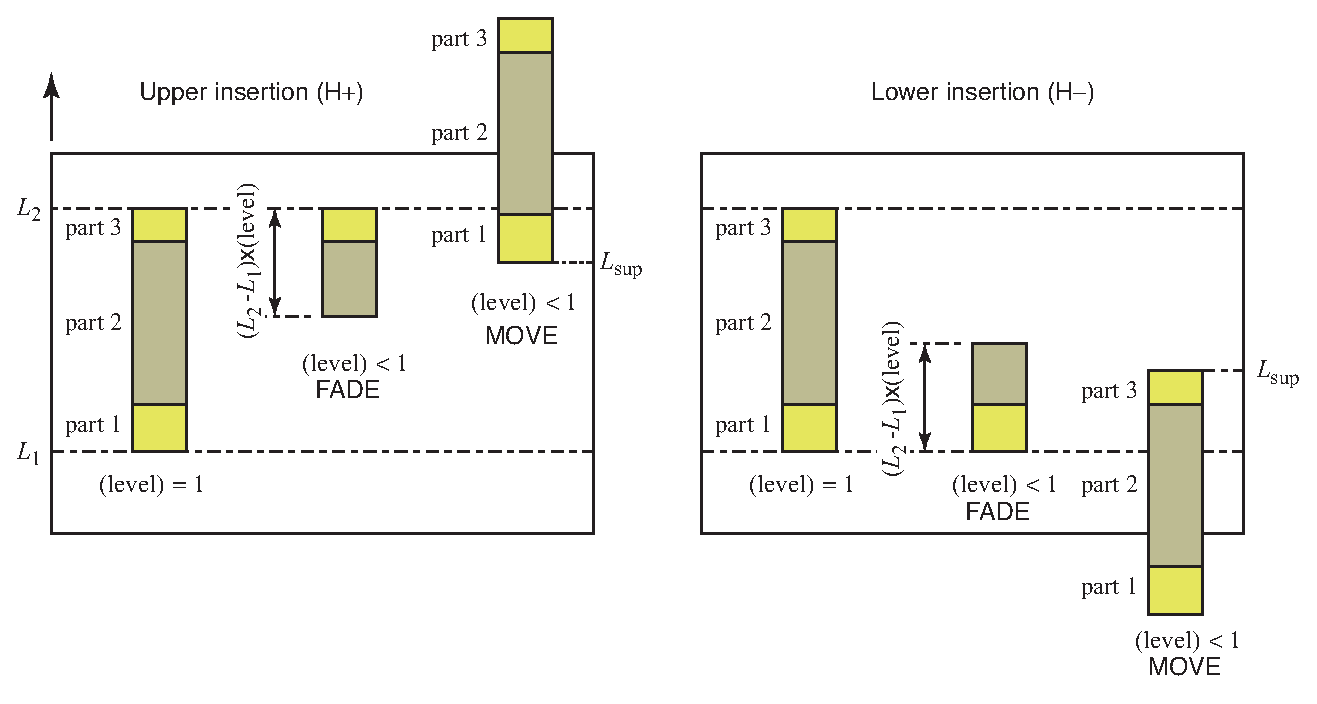
\includegraphics[scale=0.7]{Figures/rod.eps} 
\caption{Presentation of fully- and partially-inserted 3-part control rods.}\label{fig:rod}
  \end{center}
\end{figure}

\begin{DataStructure}{Structure \dstr{descdev}}
$[$ \moc{EDIT} \dusa{iprint} $]$\\
\moc{NUM-ROD} \dusa{nrod} $[~\{$ \moc{FADE} $|$ \moc{MOVE} $\}~]$ \\
( \dstr{dev-rod},  i = 1, \dusa{nrod} ) \\
$[$ \moc{CREATE}  \moc{ROD-GR} \dusa{ngrp}  ( \dstr{rod-group},  i = 1, \dusa{ngrp} ) $]$ \\
;
\end{DataStructure}

\noindent where
\begin{ListeDeDescription}{mmmmmmmm}

\item[\moc{EDIT}] keyword used to set \dusa{iprint}.

\item[\dusa{iprint}] integer index used to control the printing on screen:
= 0 for no print; = 1 for minimum printing (default value); larger values
produce increasing amounts of output.

\item[\moc{NUM-ROD}] keyword used to specify \dusa{nrod}.

\item[\dusa{nrod}] integer total number of the reactor rod-type devices.
This number must be greater than 0.

\item[\moc{FADE}] fading rod keyword. A fraction of the fully inserted rod vanishes (default option).

\item[\moc{MOVE}] moving rod keyword. The complete rod is moving (DONJON3-type movement).

\item[\moc{CREATE}] keyword used to create the rod-groups of devices.
The creation of groups is optional.

\item[\moc{ROD-GR}] keyword used to set \dusa{ngrp}.

\item[\dusa{ngrp}] integer total number of the rod groups to be created.
This number must be greater than 0.

\item[\dstr{dev-rod}] structure describing the input data for each individual rod.
 
\item[\dstr{rod-group}] structure describing the input data for each group of rods.

\end{ListeDeDescription}

\vskip 0.2cm

\subsubsection{Description of dev-rod input structure}\label{sect:devrodstr}

A rod position is referred by its \dusa{3-D} Cartesian coordinates only.
Note that the devices positions can not overlap. The input order of data
must be respected.

\begin{DataStructure}{Structure \dstr{dev-rod}}

\moc{ROD} \dusa{id} \\
~~\moc{ROD-NAME} \dusa{NAME} \\
~~\moc{AXIS} $\{$ \moc{X} $|$ \moc{Y} $|$ \moc{Z} $\}$ \\
~~\moc{FROM} $\{$ \moc{H+} $|$ \moc{H-} $\}$  \\
~~$[$ \moc{LEVEL} \dusa{value} $]$ \\
~~$[$ \moc{SPEED} \dusa{speed} $]$ \\
~~$[$ \moc{TIME} \dusa{time} $]$ \\
~~$[[$ \moc{MAXPOS}  (\dusa{pos}(i), i = 1, 6) \moc{DMIX} \dusa{mix1} \dusa{mix2} $]]$ \\
\moc{ENDROD}
\end{DataStructure}

\noindent where
\begin{ListeDeDescription}{mmmmmmmm}

\item[\moc{ROD}] keyword used to specify the rod \dusa{id} number.

\item[\dusa{id}] integer identification number of the current rod. Each
rod-type device must be assigned a unique \dusa{id} number, given in
an ascending order ranging from 1 to \dusa{nrod}.

\item[\moc{ROD-NAME}] keyword used to specify the rod \dusa{NAME}.

\item[\dusa{NAME}] \texttt{character*12} name of the current rod. In general,
this name is composed by the rod specific type (e.g. SOR, ZCR, etc.) followed
by its sequential number (e.g. 01, 02, etc.).

\item[\moc{AXIS}] keyword used to specify the rod movement axis.
A rod can be displaced along only one of the axis.

\item[\moc{X}] keyword used to specify that a rod is displaced along X axis.

\item[\moc{Y}] keyword used to specify that a rod is displaced along Y axis.

\item[\moc{Z}] keyword used to specify that a rod is displaced along Z axis.

\item[\moc{FROM}] keyword used to specify the insertion side of geometry.
The rod-devices can be inserted into the reactor core from only one side of
geometry. For example, some vertically moving devices can be inserted only
from the top, whereas other only from the bottom.

\item[\moc{H+}] keyword used to specify that a rod will be inserted into
reactor core from the highest position (e.g. from the top for vertically moving
rod-device).

\item[\moc{H-}] keyword used to specify that a rod will be inserted into
reactor core from the lowest position (e.g. from the bottom for vertically
moving rod-device).

\item[\moc{LEVEL}] keyword used to specify the actual rod insertion
level \dusa{value}. By default, the rod insertion level is left undefined.

\item[\dusa{value}] real positive value of the rod insertion level. This
value is used to compute the actual rod position in the reactor core.
The rod insertion level is minimal (\dusa{value} = 0.0) when the rod is
completely withdrawn, and it is maximal (\dusa{value} = 1.0) when the
rod is fully inserted. For the partially inserted rod the insertion level
must be: 0.0 $<$ \dusa{value} $<$ 1.0

\item[\moc{SPEED}] keyword used to specify \dusa{speed}. By default, the speed is left undefined.

\item[\dusa{speed}] real positive value of the rod movement speed,
given in cm/s. This value is needed only for the reactor regulating purpose.

\item[\moc{TIME}] keyword used to specify \dusa{time}. By default, the insertion time is left undefined.

\item[\dusa{time}] real value of time for the rod insertion (or extraction),
given in sec. This value is needed only for the reactor regulating purpose.

\item[\moc{MAXPOS}] keyword used to specify the full-inserted
coordinates of a rod part. The sequence of \moc{MAXPOS} and \moc{DMIX} data structures is
repeated for each part making the rod.

\item[\dusa{pos}] real array containing 3-D Cartesian coordinates of the
full-inserted rod. This is the limiting rod position in the reactor core, which
may or may not be the same as the actual rod position. These coordinates
must be given in the order: X$-$, X$+$, Y$-$, Y$+$, Z$-$, and Z$+$.

\item[\moc{DMIX}] keyword used to specify \dusa{mix1} and \dusa{mix2}.

\item[\dusa{mix1}] first of two integer rod mixture indices. Index \dusa{mix1} corresponds to the perturbed
cross sections.

\item[\dusa{mix2}] second of two integer rod mixture indices. Index \dusa{mix2} corresponds to the reference
cross sections. Indices \dusa{mix1} and \dusa{mix2} will be used to compute
the incremental cross sections in the \moc{NEWMAC:} module.

\item[\moc{ENDROD}] keyword used to end the rod description.

\end{ListeDeDescription}

\subsubsection{Description of rod-group input structure}\label{sect:rodgroupstr}

The partition of devices into groups is very useful when the same action is
to be applied to several rods, e.g. setting of new parameters (using the
\moc{DSET:} module) or rods moving (using the \moc{MOVDEV:} module).

\begin{DataStructure}{Structure \dstr{rod-group}}

\moc{GROUP-ID} \dusa{igrp} $\{$ \moc{ROD-ID}
$[[$ \dusa{id} $]]$  $|$  \moc{ALL} $\}$ \\

\end{DataStructure}

\noindent where
\begin{ListeDeDescription}{mmmmmmmm}

\item[\moc{GROUP-ID}] keyword used to set \dusa{igrp} number.

\item[\dusa{igrp}] integer identification number of a group to be created.
Each rods group must be assigned a unique identification number, given
in ascending order ranging from 1 to \dusa{ngrp}.

\item[\moc{ROD-ID}] keyword used to set the rod \dusa{id} numbers.

\item[\dusa{id}] integer identification numbers of rods which belong
to the same group \dusa{igrp}. A particular rod (or several rods) may
belong to different groups, but it could not be repeated inside the same
group. The total number of rods in any group must be between
1 and \dusa{nrod}.

\item[\moc{ALL}] keyword used to specify that all rods
will belong to the same group \dusa{igrp}.

\end{ListeDeDescription}
\clearpage

\vskip 1.0cm
\subsection{The \moc{DETINI:} module}\label{sect:tinst}

\vskip 0.2cm
The \moc{DETINI:} module is used to read and store detector information. 
A detector is represented by a 2-D or 3-D Cartesian/Hexagonal geometry.\\

\noindent
The \moc{DETINI:} module specification is:

\begin{DataStructure}{Structure \moc{DETINI:}}
\dusa{DETECT} \moc{:=} \moc{DETINI:}
$[$ \dusa{DETECT} $]$ \moc{::} \dstr{descdet}
\end{DataStructure}

\noindent where

\begin{ListeDeDescription}{mmmmmmmm}

\item[\dusa{DETECT}] \texttt{character*12} name of the \dds{detect} object
that will be created by the module; it will contain the detector informations.
If \dds{detect} appear on RHS, it is updated, otherwise, it is created.

\item[\dstr{descdev}] structure describing the input data to the
\moc{DETINI:} module.

\end{ListeDeDescription}

\vskip 0.2cm
\subsubsection{Input data to the \moc{DETINI:} module}\label{sect:strtinst}

\noindent
Note that the input order must be respected. \\
\begin{DataStructure}{Structure \dstr{descinidet}}
$[$ \moc{EDIT} \dusa{iprt} $]$ $[$ HEXZ $]$
\moc{NGRP} \dusa{ngrp} \\
$[[$ \moc{TYPE} \dusa{NAMTYP} \\
\moc{INFO} \dusa{ndetect} \dusa{nrep}
$\{$ \moc{SPECTRAL} ( \dusa{spec}(i), i=1,\dusa{ngrp} ) $|$
\moc{DEFAULT} $\}$  \\ 
$[$ \moc{INVCONST} ( \dusa{tinv}(i), i=1,\dusa{nrep}$-2$ ) $]$
$[$ \moc{FRACTION} ( \dusa{fract}(i), i=1,\dusa{nrep}$-1$ ) $]$ \\
( \dstr{descdet}, i=1,\dusa{ndetect} ) $]]$ \\
;
\end{DataStructure}

\noindent where
\begin{ListeDeDescription}{mmmmmmmm}

\item[\moc{EDIT}] keyword used to set \dusa{iprt}.

\item[\dusa{iprt}] index used to control the printing in module \moc{
INIDET:}. =1,2 for no print(default value); =3 for printing the contents 
of the output \dds{detect}.

\item[\moc{HEXZ}] keyword to specify that only hexagonal detectors will be 
defined.
If this keyword is absent, Cartesian detectors will be
defined. 

\item[\moc{NGRP}] keyword used to set \dusa{ngrp}.

\item[\dusa{ngrp}] number of energy groups in the calculation. It must be
equal to the number set in the \moc{MACD:} module or by the \dds{compo}
files. 

\item[\moc{TYPE}] keyword to specify the detector type.

\item[\dusa{NAMTYP}] \texttt{character*12} name of the detector type.
To correspond to the actual detector response model encoded,
the type of detector must be in this list: 
\begin{itemize}
\item  \texttt{PLATN\_REGUL}
\item  \texttt{PLATN\_SAU}
\item  \texttt{VANAD\_REGUL} 
\item  \texttt{CHION\_SAU}
\item  \texttt{CHION\_REGUL} 
\end{itemize}
For other type names, only a fixed normalisation can be performed.

\item[\moc{INFO}] keyword to specify the information associated 
with the detector type.

\item[\dusa{ndetect}] number of detectors of the specified type.

\item[\dusa{nrep}] number of detector response components for the specified 
type. It must be greater or equal to 2, corresponding to a response in
fraction and the reference flux value.
 
\item[\moc{SPECTRAL}] keyword to specify the energy spectral of
a detector type.

\item[\dusa{spec}] array containing the energy spectral of a detector type.

\item[\moc{DEFAULT}] keyword to specify the energy spectral will be
initialized as 1.0 for the highest energy group and 0.0 for other groups.

\item[\moc{INVCONST}] keyword to specify the inverse time constants of
the detector type model. This option is only valid for platinum, 
(\dusa{NAMTYP}(1:5) = 'PLATN'),
detector type. 
\item[\dusa{tinv}] array containing the inverse time constants of
the detector model.

\item[\moc{FRACTION}] keyword to specify the fractions corresponding to
each delayed or prompt reponse of the detector type model. This option is 
only valid for platinum, (\dusa{NAMTYP}(1:5) = 'PLATN'), detector type. 

\item[\dusa{frac}] array containing the detector type model fractions.

\item[\dstr{descdet}] structure describing the format used to read
detector information.
 
\end{ListeDeDescription}

\vskip 0.2cm

\subsubsection{Description of the detector data}

Note that the information input order must be respected. 

\begin{DataStructure}{Structure \dstr{descdet}}
\moc{NAME} \dusa{NAMDET} \\
$[$ \moc{NHEX} \dusa{nhex} \moc{HEX} ( \dusa{ihex}(i), i=1,\dusa{nhex} ) $]$ \\
\moc{POSITION} ( \dusa{pos}(i), i=1,6 )\\
\moc{RESP} ( \dusa{rep}(i), i=1,\dusa{nrep} )\\
\moc{ENDN} 
\end{DataStructure}

\noindent where
\begin{ListeDeDescription}{mmmmmmmm}

\item[\moc{NAME}] keyword to specify the detector name.

\item[\dusa{NAMDET}] \texttt{character*12} name of the detector.
The different names in alphabetical order must fit
their usual numbering in the core.(Ex: PLATN01, CHION01C) 

\item[\moc{NHEX}] keyword to set the number of hexagons where the detector
is placed.

\item[\dusa{nhex}] number of hexagons.

\item[\moc{HEX}] keyword to set the hexagon numbers corresponding to
the detector position.

\item[\dusa{ihex}] array containing the hexagon numbers
 where the detector is present, as ordered in the geometry definition. 

\item[\moc{POSITION}] keyword to specify the detector coordinates.

\item[\dusa{pos}] array containing the positions of the specified detector.
The positions must be read as X$-$ X+ Y$-$ Y+ Z$-$ Z+ . For 2-D geometry,
Z coordinates must be 0.0 and a value greater than 1.0. For hexagonal geometry,
only Z coordinates are used in 3-D representation.

\item[\moc{RESP}] keyword to specify the detector initial responses.

\item[\dusa{rep}] array containing the initial responses of the detector.
To use the current detector models in DONJON, responses are given as

\begin{itemize}
\item For vanadium detectors: current response, last response.
\item For platinum detectors: current response, reference flux, last
detector slow 
responses.
\item For ion chamber detectors: current logarithmic response, current
log rate response, 
reference flux.
\end{itemize}
 
\item[\moc{ENDN}] keyword to specify the end of the detector informations.

\end{ListeDeDescription}
\clearpage

\vskip 1.0cm
\subsection{The \moc{LZC:} module}\label{sect:lzc}

The \moc{LZC:} module is used for the modeling of liquid zone controllers, which
are normally presented in the CANDU6-type reactor core. The liquid zone controllers
specifications are read from the input data file. Note that this modeling can be made
after the rod-type devices have been previously defined using the \moc{DEVINI:}
module (see \Sect{dev}). In this case, the previously created \dds{device} object
will be updated by the \moc{LZC:} module; it will store the additional and separate
information with respect to the liquid controllers (see \Sect{device}). \\

The liquid zone controller specification includes several device parameters, such as:
the whole device position, water filling level, direction of filling, etc. Note that a liquid
zone controller is normally composed of two parts: one part is empty and the second
part is full-filled. The water level can be adjusted according to the control reactivity
requirements. The controllers positions are referred using \dusa{3-D}-Cartesian
coordinates. Several devices parameters can be modified using the \moc{DSET:}
module (see \Sect{dset}). The liquid controllers can also be divided into the several
user-defined groups so that they can be manipulated simultaneously.\\

\noindent
The \moc{LZC:} module specification is:

\begin{DataStructure}{Structure \moc{LZC:}}
\dusa{DEVICE} \dusa{MATEX} \moc{:=} \moc{LZC:}
$[$ \dusa{DEVICE} $]$ \dusa{MATEX} \moc{::} \dstr{desclzc}
\end{DataStructure}

\noindent where

\begin{ListeDeDescription}{mmmmmmmm}

\item[\dusa{DEVICE}] \texttt{character*12} name of the \dds{device} object.
Note, if the rod-type devices are not present in the reactor core, then \dusa{DEVICE}
object must appear only on the LHS (i.e. in create mode), it will contain the information
only with respect to the liquid zone controllers. However, if the rod-type devices
are present in the reactor core, then they must be specified first (i.e. before the
liquid controllers) using the \moc{DEVINI:} module (see \Sect{dev}). In the last
case, the \dusa{DEVICE} object must also appear on the RHS (i.e. in modification
mode), it will contain the additional and separate information with respect to the
liquid zone controllers.

\item[\dusa{MATEX}] \texttt{character*12} name of the \dds{matex} object
that will be updated by the module. The lzc-devices material mixtures are
appended to the previous material index and the lzc-devices indices are
also modified, accordingly.

\item[\dstr{desclzc}] structure describing the input data to the \moc{LZC:} module.

\end{ListeDeDescription}

\vskip 0.2cm

\subsubsection{Input data to the \moc{LZC:} module}\label{sect:lzcstr}

Note that the input order must be respected.

\begin{DataStructure}{Structure \dstr{desclzc}}
$[$ \moc{EDIT} \dusa{iprint} $]$ \\
\moc{NUM-LZC} \dusa{nlzc} \\
(\dstr{dev-lzc}, i = 1, \dusa{nlzc}) \\
$[$ \moc{CREATE}  \moc{LZC-GR} \dusa{ngrp}  (\dstr{lzc-group}, i = 1, \dusa{ngrp}) $]$ \\
;
\end{DataStructure}

\noindent where
\begin{ListeDeDescription}{mmmmmmmm}

\item[\moc{EDIT}] keyword used to set \dusa{iprint}.

\item[\dusa{iprint}] integer index used to control the printing on screen:
= 0 for no print; = 1 for minimum printing (default value); larger values
produce increasing amounts of output.

\item[\moc{NUM-LZC}] keyword used to specify \dusa{nlzc}.

\item[\dusa{nlzc}] integer total number of liquid zone controllers.
This number must be greater than 0.

\item[\moc{CREATE}] keyword used to create the lzc-groups of devices.
The creation of groups is optional.

\item[\moc{LZC-GR}] keyword used to set \dusa{ngrp}.

\item[\dusa{ngrp}] integer total number of the lzc groups to be created.
This number must be greater than 0.

\item[\dstr{dev-lzc}] structure describing the input data for each individual
liquid controller.
 
\item[\dstr{lzc-group}] structure describing the input data for each group of
liquid controllers.

\end{ListeDeDescription}

\vskip 0.2cm

\subsubsection{Description of dev-lzc input structure}\label{sect:devlzcstr}

Note that the devices positions can not overlap in the reactor core. The input order of data
must be respected.

\begin{DataStructure}{Structure \dstr{dev-lzc}}
\moc{LZC} \dusa{id} \\
\moc{MAXPOS}  ( \dusa{pos}(i) , i = 1, 6 ) \\
\moc{MAX-FULL} \dusa{fmax} \\
\moc{AXIS} $\{$ \moc{X} $|$ \moc{Y} $|$ \moc{Z} $\}$ \\
\moc{LEVEL} \dusa{value} \\
$[$ \moc{RATE} \dusa{rate} $]$ \\
$[$ \moc{TIME} \dusa{time} $]$ \\
\moc{EMPTY-MIX}  ( \dusa{mixE}(n), n = 1, 2 ) \\
\moc{FULL-MIX}  ( \dusa{mixF}(n), n = 1, 2 )
\end{DataStructure}

\noindent where
\begin{ListeDeDescription}{mmmmmmmm}

\item[\moc{LZC}] keyword used to specify the liquid controller
\dusa{id} number.

\item[\dusa{id}] integer identification number of the current liquid controller.
Each controller must be assigned a unique \dusa{id} number, given in an
ascending order ranging from 1 to \dusa{nlzc}.

\item[\moc{MAXPOS}] keyword used to specify the entire position of a
liquid zone controller, including its empty and full parts.

\item[\dusa{pos}] real array containing 3-D Cartesian coordinates of the
liquid zone controller position in the reactor core. These coordinates
must be given in the order: X$-$  X$+$   Y$-$  Y$+$   Z$-$  Z$+$

\item[\moc{MAX-FULL}] keyword used to specify \dusa{fmax}.

\item[\dusa{fmax}] real value of the limiting coordinate along the controller
filling axis, which corresponds to the maximum full-filling level for the current
liquid controller.

\item[\moc{AXIS}] keyword used to specify the controller filling axis.
A liquid controller can be filled along only one (vertical) axis.

\item[\moc{X}] keyword used to specify that a liquid controller is filled along X axis.

\item[\moc{Y}] keyword used to specify that a liquid controller is filled along Y axis.

\item[\moc{Z}] keyword used to specify that a liquid controller is filled along Z axis.

\item[\moc{LEVEL}] keyword used to specify the actual filling level.

\item[\dusa{value}] real positive value of the water level. This value is minimal
(\dusa{value} = 0.0) when the controller is empty, and it is maximal (\dusa{value} = 1.0)
when the controller is full-filled. For the partially filled controller the water level
must be: 0.0 $<$ \dusa{value} $<$ 1.0

\item[\moc{RATE}] keyword used to specify \dusa{rate}.

\item[\dusa{rate}] real positive value of the water filling rate, given in
m$^{3}$/s. This value is needed only for the reactor regulating purpose.

\item[\moc{TIME}] keyword used to specify \dusa{time}.

\item[\dusa{time}] real value of the filling time, given in sec.
This value is needed only for the reactor regulating purpose.

\item[\moc{EMPTY-MIX}] keyword used to specify \dusa{mixE}.

\item[\dusa{mixE}] two integer mixture indices, specified for the empty-part of
liquid controller. The first and the second mixture indices correspond to the
perturbed and the reference cross sections, respectively. These indices will be
used to compute the incremental cross sections in the \moc{NEWMAC:} module.

\item[\moc{FULL-MIX}] keyword used to specify \dusa{mixF}.

\item[\dusa{mixF}] two integer mixture indices, specified for the full-part of liquid
controller. The first and the second mixture indices correspond to the perturbed
and the reference cross sections, respectively. These indices will be used
to compute the incremental cross sections in the \moc{NEWMAC:} module.

\end{ListeDeDescription}
\clearpage

\subsubsection{Description of lzc-group input structure}\label{sect:lzcgroupstr}

The partition of lzc-devices into groups is similar to that of rod-devices.

\begin{DataStructure}{Structure \dstr{lzc-group}}
\moc{GROUP-ID} \dusa{igrp} $\{$ \moc{LZC-ID}
$[[$ \dusa{id} $]]$  $|$  \moc{ALL} $\}$
\end{DataStructure}

\noindent where
\begin{ListeDeDescription}{mmmmmmmm}

\item[\moc{GROUP-ID}] keyword used to set \dusa{igrp} number.

\item[\dusa{igrp}] integer identification number of a group to be created.
Each controllers group must be assigned a unique identification number,
given in ascending order ranging from 1 to \dusa{ngrp}.

\item[\moc{LZC-ID}] keyword used to set the controllers \dusa{id} numbers.

\item[\dusa{id}] integer identification numbers of the liquid controllers which
belong to the same group \dusa{igrp}. A particular controller (or several devices)
may belong to different groups, but it could not be repeated inside the same
group. The total number of liquid controllers in any group must be between
1 and \dusa{nlzc}.

\item[\moc{ALL}] keyword used to specify that all liquid controllers
will belong to the same group \dusa{igrp}.

\end{ListeDeDescription}
\clearpage

\vskip 1.0cm
\subsection{The \moc{DSET:} module}\label{sect:dset}

\vskip 0.2cm
The \moc{DSET:} module is used to set or to update some of the devices
parameters. The new parameters can be applied for the rod-type devices
and/or for the liquid zone controllers, such as: the new insertion level for the
rods or water filling level for the lzc-type devices, etc. It is possible to apply
the new parameters to the individual user-selected devices as well as to the
user-selected groups of devices. If the device (rod-insertion or lzc-filling) level
is selected for the modification, then a new device position is recomputed
accordingly. The \moc{DSET:} module can be used to perform the device
reactivity studies and also to predict the reactivity worth of the rod-devices.\\

\noindent
The \moc{DSET:} module specification is:

\begin{DataStructure}{Structure \moc{DSET:}}
\dusa{DEVICE} \moc{:=} \moc{DSET:}
\dusa{DEVICE} \moc{::} \dstr{descdset}
\end{DataStructure}

\noindent where

\begin{ListeDeDescription}{mmmmmmmm}

\item[\dusa{DEVICE}] \texttt{character*12} name of the \dds{device}
object that will be updated by the module.

\item[\dstr{descdset}] structure describing the input data to
the \moc{DSET:} module. 

\end{ListeDeDescription}

\vskip 0.2cm

\subsubsection{Input data to the \moc{DSET:} module}\label{sect:dsetstr}

It is possible to set or to modify the parameters for several individual
devices and/or for several groups of devices simultaneously.

\begin{DataStructure}{Structure \dstr{descdset}}
\moc{EDIT} \dusa{iprint} \\
$[[$  $\{$ \moc{ROD} \dusa{irod} $|$ \moc{ROD-GROUP} \dusa{irgrp}
$|$ \moc{LZC} \dusa{ilzc} $|$ \moc{LZC-GROUP} \dusa{ilgrp} $\}$ \\
$[$ \moc{LEVEL} \dusa{value} $]$
$[$ \moc{SPEED} \dusa{speed} $]$
$[$ \moc{TIME} \dusa{time} $]$ \\
 \moc{END}  $]]$ \\
;
\end{DataStructure}

\noindent where
\begin{ListeDeDescription}{mmmmmmmm}

\item[\moc{EDIT}] keyword used to set \dusa{iprint}.

\item[\dusa{iprint}] integer index used to control the printing on screen:
= 0 for no print; = 1 for minimum printing; larger values produce
increasing amounts of output.

\item[\moc{ROD}] keyword used to specify the rod \dusa{irod} number.

\item[\dusa{irod}] integer identification number of a rod to be modified.
Each rod-type device has a unique \dusa{irod} number, ranging from 1 to
\dusa{nrod}, as been defined in the \moc{DEVINI:} module (see \Sect{devrodstr}).

\item[\moc{ROD-GROUP}] keyword used to specify the rod-group
\dusa{irgrp} number.

\item[\dusa{irgrp}] integer identification number of a rod-group of devices
that will be modifed with the same parameters. Each rod-group has a unique
\dusa{irgrp} number, ranging from 1 to \dusa{ngrp}, as been defined in the
\moc{DEVINI:} module (see \Sect{rodgroupstr}).

\item[\moc{LZC}] keyword used to specify the liquid controller
\dusa{ilzc} number.

\item[\dusa{ilzc}] integer identification number of a liquid controller to be modified.
Each lzc-type device has a unique \dusa{ilzc} number, ranging from 1 to
\dusa{nlzc}, as been defined in the \moc{LZC:} module (see \Sect{devlzcstr}).

\item[\moc{LZC-GROUP}] keyword used to specify the lzc-group
\dusa{ilgrp} number.

\item[\dusa{ilgrp}] integer identification number of a lzc-group of devices
that will be modifed with the same parameters. Each lzc-group has a unique
\dusa{ilgrp} number, ranging from 1 to \dusa{ngrp}, as been defined in the
\moc{LZC:} module (see \Sect{lzcgroupstr}).

\item[\moc{LEVEL}] keyword used to specify a new level \dusa{value}.

\item[\dusa{value}] real positive value of the new device level. For the
rod-type devices this \dusa{value} must correspond to the new rod insertion
level (see \Sect{rodgroupstr}). For the lzc-type devices this \dusa{value}
must correspond to the new water filling level (see \Sect{devlzcstr}).
In any case, the new level value must be: 0.0 $\leq$ \dusa{value} $\leq$ 1.0

\item[\moc{SPEED}] keyword used to specify a new value for \dusa{speed}.

\item[\dusa{speed}] real positive value of the device speed. For the
rod-type devices this value must correspond to the speed of rod movement
(insertion or extraction), given in cm/s. For the lzc-type devices this value
must correspond to the water filling rate, given in m$^{3}$/s. The value of
\dusa{speed} is required only for the reactor regulating purpose.

\item[\moc{TIME}] keyword used to specify a new value for \dusa{time}.

\item[\dusa{time}] real value of time either for the rod insertion (or extraction)
\dusa{or} for the liquid controller filling, given in sec. The value of \dusa{time}
is required only for the reactor regulating purpose.

\item[\moc{END}] keyword used to indicate the end of input of the
new parameters for the current device or group of devices.

\end{ListeDeDescription}
\clearpage

\vskip 1.0cm
\subsection{The {\tt MCC:} module}\label{sect:MCCData}

The \moc{MCC:} module supplies tools to edit selectively one or several parameters of a fuel map object. These parameters are the ones defined when the fuel map is created, according to the calculation grid chosen to compute the macroscopic cross-sections libraries. Their selective edition is useful to study their impact on the core reactivity. For instance, this module enables to increase uniformly the fuel temperature in each cell, without modifying any other parameter such as the moderator temperature. It grants access to the Doppler coefficient, even at hot full power when the fuel temperature is different in every cell of the core.\\

This module enables the computation of (non-exhausive list) : the Doppler coefficient, the power Doppler coefficient (Doppler during a power transient), the moderator temperature coefficient, the boron concentration coefficient, the reactivity with the fuel temperature set to the moderator one, etc.\\

Note that this module does not perform any reactivity calculation (only fuel map edition).\\

The \moc{MCC:} module specifications are:

\begin{DataStructure}{Structure \moc{MCC:}}
$[$\dusa{FLMAP1}$]$ \moc{:=}
\moc{MCC:} \dusa{FLMAP1} $[$\dusa{FLMAP2}$]$ \moc{::} \dstr{descmcc1} 
\end{DataStructure}

\noindent where
\begin{ListeDeDescription}{mmmmmmmm}

\item[\dusa{FLMAP1}] \texttt{character*12} name of the \dds{MAP} object that will contain the updated fuel-lattice information. If \dusa{FLMAP1} appears on both LHS and RHS, it will be updated; if it only appears on RHS, it will only be read to display its contents.

\item[\dusa{FLMAP2}] \texttt{character*12} name of the \dds{MAP} object that contains information to be recovered to update \dusa{FLMAP1}. If \dusa{FLMAP2} exists, data to update \dusa{FLMAP1} will be taken in it. If not, data to update \dusa{FLMAP1} will be taken in \dusa{FLMAP1}.

\item[\dstr{descmcc1}] structure describing the main input data to the \moc{MCC:} module. Note that this input data is mandatory and must be specified either if \dusa{FLMAP1} is updated or only read.

\end{ListeDeDescription}

% Parameter description

\vskip 0.2cm
\subsubsection{Main input data to the \moc{MCC:} module}\label{sect:mccmain}

\noindent

\begin{DataStructure}{Structure \dstr{descmcc1}}
$[$ \moc{EDIT} \dusa{iprint} $]$\\
$[[$ \moc{REC} \dusa{rec1} $\{$ \moc{UNI} \dusa{value1} $|$ \moc{ADD} \dusa{value2} $|$ $\{$ \moc{SAME} $|$ \moc{READ} $\}$ \dusa{rec2} $\}$ $]]$ \\
$[$ \moc{TTD} \dusa{pcore} $]$\\
\moc{;}
\end{DataStructure}

\noindent where

\begin{ListeDeDescription}{mmmmmmmm}

\item[\moc{EDIT}] keyword used to set \dusa{iprint}.

\item[\dusa{iprint}] integer index used to control the printing on screen:
 = 0 for no print; = 1 for minimum printing (default value); larger values
produce increasing amounts of output. A value of 5 or higher will display 
the contents of \dusa{FLMAP1} object after edition, and a value of 6 or higher
will display the contents before edition.

\item[\moc{REC}] keyword used to indicate that the name of the record to be
updated will follow.

\item[\dusa{rec1}] name of the record to be updated. The authorised values are
defined in the table \ref{sect:dirparam}, page \pageref{sect:dirparam} (\moc{P-NAME}
variable). To be allowed, these values have to be previously defined in the fuel
map before calling \moc{MCC}.

\item[\moc{UNI}] keyword to specify that an uniform and absolute value
is to be set. With this parameter, the \dusa{rec1} of every region will have
the same value.

\item[\dusa{value1}] absolute value (in Kelvin if it is a temperature) that will
be set for \dusa{rec1} in every region.

\item[\moc{ADD}] keyword to specify that an uniform variation of \dusa{rec1} value
is to be applied. With this parameter, the value of \dusa{rec1} will be altered in
every region.

\item[\dusa{value2}] value of \dusa{rec1} variation (in Kelvin if it is a
temperature) that will be applied to every region.

\item[\moc{SAME}] keyword used to indicate that the values to edit \dusa{rec1} are
to be recovered from \dusa{rec2} in the same fuel map, \dusa{FLMAP1}. For instance,
it enables the user to set the fuel temperature with the moderator temperature.

\item[\moc{READ}] keyword used to indicate that the values to edit \dusa{rec1} are
to be recovered from \dusa{rec2} in an other fuel map, \dusa{FLMAP2}. For instance,
it enables the user to set the fuel temperature in \dusa{FLMAP1} with the fuel
temperature of \dusa{FLMAP2}.

\item[\dusa{rec2}] name of the record where the data to perform the update of 
\dusa{FLMAP1} is to be recovered. The authorised values are defined in the table
\ref{sect:dirparam}, page \pageref{sect:dirparam} (\moc{P-NAME} variable). 
To be allowed, these values have to be previously defined in the fuel
map before calling \moc{MCC}.

\item[\moc{TTD}] keyword used to indicate that the values of the {\tt 'D-COOL'}
record are to be updated. They will be computed from the moderator temperature
stored in the {\tt 'T-COOL'} folder and the core pressure, using the water tables.
Note that the position of the \moc{TTD} keyword matters, the density being
calculated when \moc{TTD} is called and not at the end of \moc{MCC:} execution.

\item[\dusa{pcore}] core pressure (in Pa).

\end{ListeDeDescription}

\eject

\vskip 1.0cm
\subsection{The \moc{MOVDEV:} module}\label{sect:movdev}

\vskip 0.2cm
The \moc{MOVDEV:} module can be used for the transient simulations and
reactor control studies, which are related to the time-dependent rod-devices
displacement in the reactor core. The rods can be inserted into or extracted
from the reactor core, at constant or at variable speed of movement. The rod
positions are recomputed at every given time step of movement. The new rod
positions can be computed in several ways, based on either: current time increment
and movement speed; relative change in rod positions; \dusa{or} current rod
insertion level. The \moc{MOVDEV:} module allows the rod-devices to be
displaced individually or simultaneously in groups.\\

\noindent
The \moc{MOVDEV:} module specification is:

\begin{DataStructure}{Structure \moc{MOVDEV:}}
\dusa{DEVICE} \moc{:=} \moc{MOVDEV:}
\dusa{DEVICE} \moc{::} \dstr{descmove}
\end{DataStructure}

\noindent where

\begin{ListeDeDescription}{mmmmmmmm}

\item[\dusa{DEVICE}] \texttt{character*12} name of the \dds{device}
object that will be modified by the module. The rods positions are updated
according to the current time step of movement.

\item[\dstr{descmove}] structure describing the input data to the
\moc{MOVDEV:} module.

\end{ListeDeDescription}

\vskip 0.2cm

\subsubsection{Input data to the \moc{MOVDEV:} module}\label{sect:movdevstr}

It is possible to move several individual rods and/or several groups of rods
simultaneously. A user must be aware that a particular device will not be displaced
more than once during the same time step. Note that the input order of data to the
module must be respected. 

\begin{DataStructure}{Structure \dstr{descmove}}
$[$ \moc{EDIT} \dusa{iprint} $]$\\
\moc{DELT} \dusa{delt} \\
$[[$ $\{$ \moc{ROD} \dusa{id} $|$
\moc{GROUP} \dusa{igrp} $\}$ \\
$\{$ \moc{INSR} $|$ \moc{EXTR} $\}$ \\
$\{$ \moc{LEVEL} \dusa{value} $|$
\moc{DELH} \dusa{delh} $|$
\moc{SPEED} \dusa{speed} $\}$ $]]$  \\
;
\end{DataStructure}

\noindent where
\begin{ListeDeDescription}{mmmmmmmm}

\item[\moc{EDIT}] keyword used to set \dusa{iprint}.

\item[\dusa{iprint}] integer index used to control the printing on
screen: = 0 for no print; = 1 for minimum printing (default value);
larger values produce increasing amounts of output.

\item[\moc{DELT}] keyword used to set \dusa{delt}.

\item[\dusa{delt}] real value of the time increment for the current
time step, given in sec.

\item[\moc{ROD}] keyword used to specify the rod \dusa{id} number.

\item[\dusa{id}] integer identification number of a rod-type device to be
displaced. Each rod has a unique \dusa{id} number, ranging from 1 to
\dusa{nrod}, as been defined in the \moc{DEVINI:} module (see \Sect{devrodstr}).

\item[\moc{GROUP}] keyword used to specify a rod-group \dusa{igrp} number.

\item[\dusa{igrp}] integer number of a group of rods that will be displaced
simultaneously, with the same parameters of movement. Each group of
rod-devices has a unique \dusa{igrp} number, ranging from 1 to \dusa{ngrp},
as been defined in the \moc{DEVINI:} module (see \Sect{rodgroupstr}).

\item[\moc{INSR}] keyword used to specify that a particular rod or a
group of rods will be inserted into the reactor core during the period
of time \dusa{delt}.

\item[\moc{EXTR}] keyword used to specify that a particular rod or a
group of rods will be extracted from the reactor core during the period
of time \dusa{delt}.

\item[\moc{LEVEL}] keyword used to specify the new level \dusa{value}.

\item[\dusa{value}] real positive value of the rod insertion level at current
time step. This value will be used to compute the new rod position in the
reactor core. The insertion level is minimal (\dusa{value} = 0.0) when the
rod is completely withdrawn, and it is maximal (\dusa{value} = 1.0) when
the rod is fully inserted. For the partially inserted rod the insertion level
must be: 0.0 $<$ \dusa{value} $<$ 1.0

\item[\moc{DELH}] keyword used to specify the value \dusa{delh}.

\item[\dusa{delh}] real positive (absolute) value of the relative change in the
rod position during the period of time \dusa{delt}. This is a time-dependent
rod displacement along the rod movement axis, which must be given in cm.

\item[\moc{SPEED}] keyword used to set the current value of \dusa{speed}.

\item[\dusa{speed}] real positive (absolute) value of the rod movement
speed, given in cm/s. The rod speed can be kept constant or it can be
modified at any time step \dusa{delt}. The devices could also have the
different speeds of movement.

\end{ListeDeDescription}
\clearpage

\vskip 1.0cm
\subsection{The \moc{NEWMAC:} module}\label{sect:newmac}

\vskip 0.2cm
The \moc{NEWMAC:} module is used to create a complete \dds{macrolib}
with respect to the devices parameters. The resulting \dds{macrolib} will
contain the exact properties for every material region, over the whole
mesh-splitted reactor geometry. The material properties of each region are
recomputed with respect to the actual position of each rod-type and if present
lzc-type device. The computing algorithm is based on the determination of the
volumic fraction occupied by each device; the incremental cross sections are then
adjusted, accordingly. Note that the \moc{NEWMAC:} module must be executed
each time the devices positions are modified from the previously computed ones.\\

\noindent
The \moc{NEWMAC:} module specification is:

\begin{DataStructure}{Structure \moc{NEWMAC:}}
\dusa{MACRO3} \dusa{MATEX} \moc{:=} \moc{NEWMAC:}
\dusa{MATEX} \dusa{MACRO2} \dusa{DEVICE}
\moc{::} $[$ \moc{EDIT} \dusa{iprint} $]~[$ \moc{XFAC} \dusa{xfac} $]$ ;
\end{DataStructure}

\noindent where
\begin{ListeDeDescription}{mmmmmmmm}

\item[\dusa{MACRO3}] \texttt{character*12} name of the \dds{macrolib}
to be created by the module. It will contain the updated properties of each
material region with respect to the current position of each device.

\item[\dusa{MATEX}] \texttt{character*12} name of the \dds{matex} object,
containing the complete reactor material index including devices. \dusa{MATEX}
must be specified in the modification mode; it will store the updated h-factors,
computed per each fuel region with respect to the devices positions.

\item[\dusa{MACRO2}] \texttt{character*12} name of the read-only extended
\dds{macrolib}, previously created by the \moc{MACINI:} module.

\item[\dusa{DEVICE}] \texttt{character*12} name of the read-only
\dds{device} object containing the devices information and parameters.

\item[\moc{EDIT}] keyword used to set \dusa{iprint}.

\item[\dusa{iprint}] integer index used to control the printing on screen: = 0
for no print; = 1 for minimum printing; larger values produce increasing amounts
of output. The default value is \dusa{iprint} = 1.

\item[\moc{XFAC}] keyword used to specify the number of cells on which incremental cross sections were computed 
in the supercell code.

\item[\dusa{xfac}] corrective factor for delta sigmas (real number). For DRAGON code, \dusa{xfac} is generally set to 2.0 and, for MULTICELL 
code, set to 1.0 . The default value is 2.0. 

\end{ListeDeDescription}
\clearpage

\vskip 1.0cm
\subsection{The \moc{FLPOW:} module}\label{sect:flpow}

\vskip 0.2cm
The \moc{FLPOW:} module is used to compute and print the flux and power
distributions over the reactor core. It also computes and prints some additional
information, for example: the fluxes ratios with respect to the thermal energy-group
fluxes; the mean power density; the power- and flux-form factors; etc. The computed
fluxes and powers are printed either on files or on the screen. Note that the calculation
using the \moc{FLPOW:} module can be performed once the numerical solution has
been previously established using the \moc{FLUD:} or \moc{KINSOL:} module.\\

According to the user-selected module specification, the average fluxes and
powers can be computed per each fuel region over the fuel lattice \dusa{and/or}
per each material region over the whole reactor geometry. In either case, all fluxes
are normalized to the given total reactor power corresponding to the reactor nominal
conditions at core equilibrium. If the reactor is perturbed from its initial state, then a
new total reactor power can be recomputed and, accordingly, the flux and power
distributions will be updated using the previously computed normalization factor.\\

The \moc{FLPOW:} module will create a new \moc{POWER} object that will store
the information related to the reactor fluxes and powers (see \Sect{power}). In addition,
the \moc{POWER} object will store several parameters that can be used as power
and criticity constraints for the optimization and fuel management purposes, namely:
the maximum channel and bundle powers; the channel and bundle power-form factors;
the effective multiplication factor (recovered from the \dds{flux} or \dds{kinet} data structure).\\

\noindent
The \moc{FLPOW:} module specifications are:

\begin{DataStructure}{Structure \moc{FLPOW:}}
$\{$ \\
~~~\dusa{POWER} $[$ \dusa{NRMFLUX} $]~[$ \dusa{FMAP} $]$ \\
~~~~~~~~\moc{:=} \moc{FLPOW:}  $[$ \dusa{POWOLD} $]$ \dusa{FMAP}
$\{$ \dusa{FLUX} $|$ \dusa{KINET} $\}$ \dusa{TRACK} \dusa{MATEX} $[$ \dusa{MACRO} $]$ \\
~~~~~~~~\moc{::} \dstr{descflpow} \\
$|$ \\
~~~\dusa{POWER} \moc{:=} \moc{FLPOW:}  $[$ \dusa{POWOLD} $]$
$\{$ \dusa{FLUX} $|$ \dusa{KINET} $\}$ \dusa{TRACK} \dusa{MACRO} \\
~~~~~~~~\moc{::} \dstr{descflpow} \\
 $\}$
 \end{DataStructure}

\noindent where

\begin{ListeDeDescription}{mmmmmmmm}

\item[\dusa{POWER}] \texttt{character*12} name of the \dds{power} object
that will be created by the module. It will contain the information related to the
reactor fluxes and powers.

\item[\dusa{NRMFLUX}] \texttt{character*12} name of the \dds{flux} object,
in creation mode. According to the chosen option, this object contains either 
the fluxes normalized to the given total reactor power or the fluxes per bundle. 
Is it useful if you want to compute the detectors readings with the \moc{DETECT:} module.

\item[\dusa{POWOLD}] \texttt{character*12} name of the read-only \dds{power}
object. It must contain the previously computed flux normalization factor, which
corresponds to the reactor nominal or equilibrium conditions.

\item[\dusa{FMAP}] \texttt{character*12} name of the \dds{fmap} object
containing the fuel lattice specification. When \dusa{FMAP} is specified on the RHS,
the fluxes and powers calculations are performed over the fuel lattice as well
as over the whole reactor geometry. If \dusa{FMAP} is specified on the LHS, its
records \moc{'BUND-PW'} and \moc{'FLUX-AV'} will be set according to the
information present in \dusa{POWER}.

\item[\dusa{FLUX}] \texttt{character*12} name of the \dds{flux} object,
previously created by the \moc{FLUD:} module. The numerical flux solution
contained in \dusa{FLUX} is recovered and all flux are normalized to the
given total reactor power.

\item[\dusa{KINET}] \texttt{character*12} name of the \dds{kinet} object,
previously created by the \moc{KINSOL:} module. The numerical flux solution
contained in \dusa{KINET} is recovered.

\item[\dusa{TRACK}] \texttt{character*12} name of the \dds{track} object,
created by the \moc{TRIVAT:} module. The information stored in \dusa{TRACK}
is recovered and used for the average flux calculation.

\item[\dusa{MATEX}] \texttt{character*12} name of the \dds{matex} object,
containing the reactor material index and the h-factors that will be recovered
and used for the power calculation.

\item[\dusa{MACRO}] \texttt{character*12} name of the \dds{macrolib} object,
containing the h-factors that will be recovered and used for the power calculation.

\item[\dstr{descflpow}] structure describing the input data to the \moc{FLPOW:}
module .

\end{ListeDeDescription}

\vskip 0.2cm

\subsubsection{Input data to the \moc{FLPOW:} module}

\noindent
Note that the fuel-lattice power distribution can be printed only on the screen.\\

\begin{DataStructure}{Structure \dstr{descflpow}}

$[$ \moc{EDIT} \dusa{iprint} $]$ \\
$[~\{$ \moc{PTOT} \dusa{power}  $|$  \moc{P-NEW} $\}~]$ \\
$[$ \moc{FSTH} \dusa{fsth} $]~[$ \moc{INIT} $]$ \\
$[~\{$ \moc{NORM}  $|$  \moc{BUND} $\}~]$ \\
$[$ \moc{PRINT} $\{$ \moc{MAP} $|$ \moc{DISTR} $[$ \moc{FLUX} $]$
$[$ \moc{RATIO} $]$ $[$ \moc{POWER} $]$ $|$ \moc{ALL} $\}$ $]$ \\
;
\end{DataStructure}

\noindent where
\begin{ListeDeDescription}{mmmmmmmm}

\item[\moc{EDIT}] keyword used to set \dusa{iprint}.

\item[\dusa{iprint}] integer index used to control the printing on screen:
 = 0 for no print; = 1 for minimum editing (default value); = 2 only channel powers in radial
plane are printed; = 3 only bundle powers per each radial plane are printed; = 10 only bundle powers per each channel are printed. Any combination of the values 2, 3 and 10 is possible, for example 5 = 2+3. Note that any other value of \dusa{iprint} behaves as the first lower possible value, for example 7 gives the same output as 5. Moreover channel and bundle powers can be printed only if the \dusa{FMAP} object was provided in the calling specification.

\item[\moc{PTOT}] keyword used to specify the input of \dusa{power}. By default, a power is recovered from the \dusa{KINET} object.

\item[\dusa{power}] real total reactor power, given in MW. This value
must correspond to the reactor nominal conditions.

\item[\moc{FSTH}] keyword to specify the thermal to fission power ratio.

\item[\dusa{fsth}] thermal to fission power ratio. By default this value is not used, and the total
power is the one given after the \moc{PTOT} keyword.

\item[\moc{INIT}] keyword used to save the actual power distribution in the {\tt BUND-PW-INI}
record of the fuel map object \dusa{FMAP}. It is used by the \moc{AFM:} module to apply power
feedback during a fast transient using the initial power distribution instead of the actual power.

\item[\moc{P-NEW}] keyword used to indicate that a new total reactor power
is to be recomputed, based on the previously calculated flux normalization factor.
The flux and power distributions over the reactor core are updated, accordingly.
Note that this option is valid only if a read-only \dusa{POWOLD} object is provided.

\item[\moc{PRINT}] keyword used to indicate the printing on files. Note
that all produced files will have the same extension ``\moc{.res}".

\item[\moc{MAP}] keyword used to specify the printing of the average fluxes
and flux ratios per fuel bundle. The normalized bundle fluxes are computed
and printed for each reactor channel and per each energy group. The flux
ratios are computed with respect to the thermal energy-group fluxes; they
are printed on the same file.

\item[\moc{DISTR}] keyword used to indicate the printing of data
computed over the whole reactor geometry. 

\item[\moc{FLUX}] keyword used to specify the printing of flux distribution.
The normalized fluxes are printed in separated files, one file per energy
group; the number of produced files will then equal to the total number
of energy groups. The flux values are printed for each mesh-splitted volume,
in X, Y and Z planes; the virtual regions will have the fluxes values set to 0.

\item[\moc{RATIO}] keyword used to specify the printing of flux-ratio
distribution. The flux ratios are computed with respect to the thermal
energy-group fluxes per each mesh-splitted volume. They are printed
in separated files; the number of produced files will equal to the total
number of energy groups less one.

\item[\moc{POWER}] keyword used to specify the printing of power
distribution. The power values are printed for each mesh-splitted volume,
in X, Y, and Z planes; the non-fuel regions will have the power values set to 0.

\item[\moc{ALL}] keyword used to indicate the printing of all available
information, i.e. without particular selection of data.

\item[\moc{NORM}] keyword to specify that the output flux object will contain a value per mesh-splitted element, normalized 
to the given power, as required by the \moc{DETECT:} module. This is the default option.

\item[\moc{BUND}] keyword to specify that the output flux object will contain a value per bundle, normalized 
to the given power.

\end{ListeDeDescription}
\clearpage

\vskip 1.0cm
\subsection{The \moc{TAVG:} module}\label{sect:tavg}

\vskip 0.2cm
The \moc{TAVG:} module is used to compute the burnup integration limits for each
fuel bundle, the axial power-shape over the fuel lattice, the channel refuelling rates
and the reactor core-average exit burnup. All calculations using the \moc{TAVG:}
module are performed according to the time-average model for the equilibrium-core
conditions. The computing algorithm is based on bidirectional refuelling schemes of
channels and average exit burnups specified over the fuel lattice, which should be
recorded in the fuel map using the \moc{RESINI:} module.\\

Note that the complete time-average calculation is a complex and iterative procedure,
requiring of several full-core calculations (external iterations) to be performed. The main
steps of the time-average calculation using DONJON are briefly described at the end
of this section. The \moc{TAVG:} module can also be used to compute the instantaneous
fuel burnups according to the channel patterned-age-model, for the fuel management
and optimization purposes.\\

\noindent
The \moc{TAVG:} module specification is: 

\begin{DataStructure}{Structure \moc{TAVG:}}
\dusa{FMAP} \moc{:=} \moc{TAVG:} \dusa{FMAP}
\dusa{POWER} \moc{::} \dstr{desctavg}
\end{DataStructure}

\noindent where

\begin{ListeDeDescription}{mmmmmmmm}

\item[\dusa{FMAP}] \texttt{character*12} name of a \dds{fmap} object,
that will be updated by the \moc{TAVG:} module. The \dusa{FMAP} object
must contain the average exit burnups and refuelling schemes of channels.

\item[\dusa{POWER}] \texttt{character*12} name of a \dds{power} object
containing the channel and bundle powers, previously computed by the
\moc{FLPOW:} module. The channel and bundle powers are used by the
\moc{TAVG:} module to compute the normalized axial power-shape over
each channel. 

\item[\dstr{desctavg}] structure describing the input data to the \moc{TAVG:} module.

\end{ListeDeDescription}

\vskip 0.2cm
\subsubsection{Input data to the \moc{TAVG:} module}\label{sect:strtavg}

\noindent
Note that the input order must be respected. \\

\begin{DataStructure}{Structure \dstr{desctavg}}
$[$ \moc{EDIT} \dusa{iprint} $]$ \\
$[$ \moc{AX-SHAPE} $[$ \moc{RELAX} \dusa{relval} $]$ $]$ \\
$[$ \moc{B-EXIT} $]$ \\
 ;
\end{DataStructure}

\noindent where
\begin{ListeDeDescription}{mmmmmmmm}

\item[\moc{EDIT}] keyword used to set \dusa{iprint}.

\item[\dusa{iprint}] integer index used to control the printing on screen:
 = 0 for no print; = 1 for minimum printing (default value); = 2 only the burnup limits
over each channel are printed; = 3 only the axial power-shape values over each channel
are printed; = 4 only the channel refuelling rates are printed; for larger values of
\dusa{iprint} everything will be printed.

\item[\moc{AX-SHAPE}] keyword used to indicate the calculation of the new
axial power-shape and corresponding burnups limits over each reactor channel.

\item[\moc{RELAX}] keyword used to set the relaxation parameter \dusa{relval}.

\item[\dusa{relval}] real value of the relaxation parameter, generally used to
control the axial-shape convergence over the external time-average iterations.
The optimal value, which corresponds to the minimal total number of such iterations,
can be found by performing several runs at different \dusa{relval}. The default
value of the relaxation parameter is set to 0.5

\item[\moc{B-EXIT}] keyword used to indicate the calculation of the core-average
exit burnup and the channel refuelling rates.

\end{ListeDeDescription}

\vskip 0.2cm
\subsubsection{Time-average calculation using DONJON}

When the average exit burnups are provided for each channel, the exact
burnup integration limits for each fuel bundle are unknown and need to be
determined. The burnups integration limits are function of the normalized
axial power-shape, which in turn depends on the flux solution over the fuel
lattice. Moreover, the flux solution depends on the fuel-map macrolib (i.e.
fuel properties), which in turn depends on the burnups integration limits for
each fuel bundle. Consequently, the time-average calculation is an iterative
procedure that consists to repeat all the steps required for the axial power-shape
computation. This repetition is to be made until the relative error between
the two (successives) axial power-shape calculations becomes as small
as required for the precision.\\

\noindent
The axial power-shape computing scheme is composed of several steps,
each step is performed using an appropriate DONJON or TRIVAC module:

\begin{enumerate}
\item An initial axial power-shape is set as a flat distribution over the fuel
lattice and the first burnup integration limits are calculated approximately,
using the \moc{RESINI:} module. 
\item A time-average integration is performed and a new fuel-map \dds{macrolib}
is created, using either \moc{NCR:}, \moc{CRE:} or \moc{AFM:} module.
\item An extended \dds{macrolib} over the whole reactor geometry is created,
using the \moc{MACINI:} module.
\item If the devices are inserted into the reactor core, then the previously
created \dds{macrolib} is to be updated for the devices properties using the
\moc{NEWMAC:} module. 
\item The complete \dds{macrolib} is subsequently used by the \moc{TRIVAA:}
module in order to create a matrix \dds{system}. 
\item The full-core numerical solution (i.e. fluxes and effective multiplication factor)
is computed, using the \moc{FLUD:} module.
\item The channel and bundle powers are next calculated, using the
\moc{FLPOW:} module. 
\item Finally, the new axial power-shape and burnup limits are computed,
using the \moc{TAVG:} module.
\end{enumerate}

\vskip 0.1cm
\noindent
Note that the steps from 2 to 8 are to be repeated until the required precision
for the axial power-shape convergence is satisfied.

\clearpage

\vskip 1.0cm
\subsection{The \moc{TINST:} module}\label{sect:tinst}

\vskip 0.2cm
The \moc{TINST:} module is used to compute the instantaneous burnup for each fuel bundle.
You can also use \moc{TINST:} to refuel your reactor, according to a refueling-scheme. 
The scheme can be either specified with \moc{RESINI:}, or directly in \moc{TINST:}.\\

\noindent
The \moc{TINST:} module specification is:

\begin{DataStructure}{Structure \moc{TINST:}}
$\{$ \dusa{FMAP} \moc{:=} \moc{TINST:} \dusa{FMAP}
$[$ \dusa{POWER} $]~|$ \\~~
\dusa{MICLIB3} \dusa{FMAP} \moc{:=} \moc{TINST:} \dusa{FMAP} \dusa{MICLIB2}
\dusa{MICLIB} $\}$ \\


\moc{::} \dstr{desctinst}
\end{DataStructure}

\noindent where

\begin{ListeDeDescription}{mmmmmmmm}

\item[\dusa{FMAP}] \texttt{character*12} name of a \dds{fmap} object,
that will be updated by the \moc{TINST:} module. The \dusa{FMAP} object
must contain the instantaneous burnups for each fuel bundle and the weight of
each fuel mixture.

\item[\dusa{POWER}] \texttt{character*12} name of a \dds{power} object
containing the channel and bundle powers, previously computed by the
\moc{FLPOW:} module. The channel and bundle powers are used by the
\moc{TINST:} module to compute the new burn-up of each bundle. If bundle-powers are
previously specified with the module \moc{RESINI:}, you can refuel
your core without a \dusa{POWER} object.

\item[\dusa{MICLIB3}] \texttt{character*12} name of a \dds{library} object,
that will be created by the \moc{TINST:} module. This \dds{MICROLIB} contains the fuel properties after refueling when keyword MICRO is used in \dstr{desctinst}.

\item[\dusa{MICLIB2}] \texttt{character*12} name of a \dds{library} object,
that will be read by the \moc{TINST:} module. This must be a fuel-map \dusa{LIBRARY} created either created by the \moc{NCR:} or the \moc{EVO:} module.

\item[\dusa{MICLIB}] \texttt{character*12} name of a \dds{library} object,
that will be read by the \moc{TINST:} module. This \dds{MICROLIB} contains the new fuel properties, that should be used for the refueling.

\item[\dstr{desctinst}] structure describing the input data to the \moc{TINST:} module.

\end{ListeDeDescription}

\clearpage

\vskip 0.2cm
\subsubsection{Input data to the \moc{TINST:} module}\label{sect:strtinst}

\noindent
Note that the input order must be respected. \\

\begin{DataStructure}{Structure \dstr{desctinst}}
$[$ \moc{EDIT} \dusa{iprint} $]$ \\
$[$ \moc{BURN-STEP} \dusa{rburn}  $|$ \moc{TIME} \dusa{rtime} $\{$ \moc{DAY} $|$ \moc{HOUR} $|$ \moc{MINUTE} $|$ \moc{SECOND} $\}$ $]$ \\
$[[$ \moc{REFUEL} $[$ \moc{MICRO} $]$ \moc{CHAN} \dusa{NAMCHA} \dusa{nsh} $]]$ \\
$[[$ \moc{NEWFUEL} $[$ \moc{MICRO} $]$ \moc{CHAN} \dusa{NAMCHA} \dusa{nsh} $\{$ \moc{SOME}
( \dusa{imix}(i), i=1,ABS(\dusa{nsh}) ) $|$ \moc{ALL} \dusa{imix} $\}~]]$ \\
$[[$ \moc{SHUFF} \moc{CHAN} \dusa{NMCHA1} \moc{TO} 
$\{$ \dusa{NMCHA2} $|$ \moc{POOL} $\}$ $]]$ \\
$[$ \moc{PICK}  {\tt >>} \dusa{burnup} {\tt <<} $]$ \\
{\tt ;}
\end{DataStructure}

\noindent where
\begin{ListeDeDescription}{mmmmmmmm}

\item[\moc{EDIT}] keyword used to set \dusa{iprint}.

\item[\dusa{iprint}] integer index used to control the printing on screen:
 = 0 for no print; = 1 for minimum printing (default value); = 2 only the burnup limits
over each channel are printed; = 3 only the axial power-shape values over each channel
are printed; = 4 only the channel refueling rates are printed; for larger values of
\dusa{iprint} everything will be printed.

\item[\moc{BURN-STEP}] keyword used to indicate an increase of core average burn-up.

\item[\dusa{rburn}] keyword used to indicate in MWd/t the average increase
of burn-up in the core.

\item[\moc{TIME}] keyword used to indicate the time of combustion at the power specified
in \dusa{POWER} structure.

\item[\dusa{rtime}] keyword used to set the time combustion value in \moc{DAY} or \moc{HOUR}
or \moc{MINUTE} or \moc{SECOND}.

\item[\moc{DAY}] keyword used to specify that \dusa{rtime} is a number of days.

\item[\moc{HOUR}] keyword used to specify that \dusa{rtime} is a number of hours.

\item[\moc{MINUTE}] keyword used to specify that \dusa{rtime} is a number of minutes.

\item[\moc{SECOND}] keyword used to specify that \dusa{rtime} is a number of seconds.

\item[\moc{REFUEL}] key word to specify a channel refueling.

\item[\moc{MICRO}] keyword used to perform a microscopic refueling. In this case, three libraries have to be provided when \moc{TINST:} is called.

\item[\moc{CHAN}] key word to specify the refueled channel information.

\item[\dusa{NAMCHA}] channel name. In Cartesian geometry, \dusa{NAMCHA} is a character*4 variable defined by \dusa{NXNAME} and
\dusa{NYNAME} and constructed as \\
{\tt WRITE(NAMCHA,'(A1,A3)')} \dusa{NYNAME}(1:1),\dusa{NXNAME}(1:2).

\item[\dusa{nsh}] refueling scheme. The absolute value of \dusa{nsh} is
the number of fuel bundles inserted in the channel \dusa{NAMCHA}.
The sign of \dusa{nsh} define the refueling direction: positive direction
is from the first to the \dusa{nk}-th bundle and negative is from the 
\dusa{nk}-th to the first bundle.

\item[\moc{NEWFUEL}] key word to specify that a channel will be refueled
with a different type of fuel.

\item[\moc{SOME}] key word to specify that the \dusa{nsh} values of
fuel types can be different.

\item[\dusa{imix}(i)] index number of a fuel type with respect to the
values defined in module \moc{NCR:}, \moc{CRE:} or \moc{AFM:}.

\item[\moc{ALL}] key word to specify that the \dusa{nsh} values of
fuel types will be identical to \dusa{imix}.

\item[\moc{SHUFF}] key word to specify that a specified channel will
move into an other one or discharge into the pool.

\item[\moc{CHAN}] key word to specify the moved channel name.

\item[\dusa{NMCHA1}] channel name as defined by \dusa{NXNAME} and
\dusa{NYNAME}. It is constructed as \dusa{NAMCHA}. 

\item[\moc{TO}] key word to specify the bundle destination.

\item[\dusa{NMCHA2}] channel name as defined by \dusa{NXNAME} and
\dusa{NYNAME}. It is constructed as \dusa{NAMCHA}. 

\item[\moc{POOL}] key word to specify that the channel referenced by
\dusa{NMCHA1} is discharged into the pool.

\item[\moc{PICK}]  keyword used to recover the final burnup value (in MW-day/tonne) in a CLE-2000 variable.

\item[\dusa{burnup}] \texttt{character*12} CLE-2000 variable name in which the extracted burnup value will be placed.

\end{ListeDeDescription}
\clearpage

\vskip 1.0cm
\subsection{The \moc{SIM:} module}\label{sect:sim}

\vskip 0.2cm
The \moc{SIM:} module can perform a sequence of operations related to
fuel management in PWRs:
\begin{itemize}
\item simulate a refuelling and shuffling scheme and update the burnup distribution
accordingly. The refuelling scheme is specified directly in \moc{SIM:}.
\item increase the burnup using the power available in the \dusa{POWER} object
and compute the final instantaneous burnup of each assembly subdivision
\item modify a local parameter such as the Boron concentration in the coolant.
\end{itemize}

\noindent
The \moc{SIM:} module specification is:

\begin{DataStructure}{Structure \moc{SIM:}}\label{table:tsim}
\dusa{FMAP} $[$ \dusa{MLIB} $]$ \moc{:=} \moc{SIM:} \dusa{FMAP} $[$ \dusa{MLIB} $]~[$ \dusa{POWER} $]$ \\
\moc{::} \dstr{descsim}
\end{DataStructure}

\noindent where

\begin{ListeDeDescription}{mmmmmmmm}

\item[\dusa{FMAP}] \texttt{character*12} name of a \dds{fmap} object,
that will be updated by the \moc{SIM:} module. The \dusa{FMAP} object
must contain the instantaneous burnups for each assembly subdivision, a basic naval-coordinate
assembly layout and the weight of each assembly subdivision.

\item[\dusa{MLIB}] {\tt character*12} name of a {\sc microlib} (type {\tt L\_LIBRARY}) containing particularized isotope data. If this
object also appears on the RHS, it is open in modification mode and updated. Number densities of isotopes present in list \dusa{HISOT}
(see Sect.~\ref{sect:resinimain}) are recovered from a fuel cycle information directory of \dusa{FMAP} and saved in \dusa{MLIB} or
recovered from \dusa{MLIB} and saved in a fuel cycle information directory of \dusa{FMAP}.

\item[\dusa{POWER}] \texttt{character*12} name of a \dds{power} object
containing the channel and powers of the assembly subdivisions, previously computed by the
\moc{FLPOW:} module. The channel and powers of the assembly subdivisions are used by the
\moc{SIM:} module to compute the new burn-up of each assembly subdivision. If the powers
of the assembly subdivisions are previously specified with the module \moc{RESINI:}, you can burn
your core without a \dusa{POWER} object.

\item[\dstr{descsim}] structure describing the input data to the \moc{SIM:} module.

\end{ListeDeDescription}

\vskip 0.2cm
\subsubsection{Input data to the \moc{SIM:} module}\label{sect:strsim}

\noindent
Note that the input order must be respected.

\begin{DataStructure}{Structure \dstr{descsim}}
$[$ \moc{EDIT} \dusa{iprint} $]$ \\
$[$ \moc{CYCLE} \dusa{hcnew} $[$ \moc{FROM}  \dusa{hcold} $[$ \moc{BURN} $\{$ \dusa{indcycle} $|$ \dusa{burncycle} $\}~]~]$ \\
~~~~~$[~\{$ \moc{MAP} (\dusa{hx}(i), i=1, \dusa{lx} ) \\
~~~~~~~~~~~~       (\dusa{hy}(j), (\dusa{hcase}(i,j), i=1, \dusa{lx} ), j=1,ly ) $|$ \\
~~~~~~ \moc{QMAP} (\dusa{hx}(i), i=\dusa{lx}/2+1, \dusa{lx} ) \\
~~~~~~~~~~~~~       (\dusa{hy}(j), (\dusa{hcase}(i,j), i=\dusa{lx}/2+1, \dusa{lx} ), j=\dusa{ly}/2+1,ly ) $\}~]$ \\
~~~~~$[$ \moc{SPEC} $[[~[[$ \dusa{asmb1} $]]$ \\
~~~~~~~~$\{$ \moc{SET} \moc{AVGB} \dusa{avburn} $|$ \moc{SET} \moc{FUEL} \dusa{ifuel} $|$ \moc{FROM} \dusa{hcold2} \moc{AT} \dusa{asmb2} $[$ \moc{BURN} $\{$ \dusa{indcycle} $|$ \dusa{burncycle} $\}~]~\}$ \\
~~~~~~~~~~~~~~$]]~]$ \\
~~~~~$[$ \moc{DIST-AX} $[[~[[$ \dusa{asmb1} $]]$ \\
~~~~~~~~$\{$  \moc{SET} (\dusa{axn}(i), i=1,\dusa{nb}) $|$ \moc{FROM} \dusa{hcold2} \moc{AT} \dusa{asmb2} $[$ \moc{BURN} $\{$ \dusa{indcycle} $|$ \dusa{burncycle} $\}~]~\}$ \\
~~~~~~~~~~~~~~~~~~~$]]~]$ \\
~~~~~$[$ \moc{BURN-STEP} \dusa{rburn}  $|$ \moc{TIME} \dusa{rtime} $\{$ \moc{DAY} $|$ \moc{HOUR} $|$ \moc{MINUTE} $|$ \moc{SECOND} $\}$ $]$ \\
~~~~~$[$ \moc{SET-FOLLOW} $[$ \moc{BURN} $\{$ \dusa{indcycle} $|$ \dusa{burncycle} $\}~]~]$ \\
\moc{ENDCYCLE} $]$ \\
$[[$ \moc{COMPARE} \dusa{hc1} $[$ \moc{BURN} $\{$ \dusa{indcycle1} $|$ \dusa{burncycle1} $\}~]$ \dusa{hc2} $[$ \moc{BURN} $\{$ \dusa{indcycle2} $|$ \dusa{burncycle2} $\}~]$ \\
~~~~~~~$\{$ \moc{DIST-BURN}  {\tt >>} \dusa{epsburn} {\tt <<}  $|$ \moc{DIST-POWR}  {\tt >>} \dusa{epspowr} {\tt <<} $\}~]]$ \\
$[[$ \moc{SET-PARAM} \dusa{PNAME} \dusa{pvalue} $]]$ \\
;
\end{DataStructure}

\noindent where
\begin{ListeDeDescription}{mmmmmmmm}

\item[\moc{EDIT}] keyword used to set \dusa{iprint}.

\item[\dusa{iprint}] integer index used to control the printing on screen:
 = 0 for no print; = 1 for minimum printing (default value); for larger values of
\dusa{iprint} everything will be printed.

\item[\moc{CYCLE}] keyword defining operations based on the actual fuel cycle.

\item[\dusa{hcnew}] \texttt{character*12} identification name of the specific fuel cycle.

\item[\moc{FROM}] keyword defining the previous fuel cycle in case that some information
needs to be transmitted to the actual fuel cycle.

\item[\dusa{hcold}] \texttt{character*12} identification name of the previous fuel cycle.

\item[\moc{BURN}] keyword defining the burnup at which the assembly is recycled in the previous fuel cycle. By default, the
last burnup step is used.

\item[\dusa{indcycle}] integer index of the burnup step in the previous fuel cycle.

\item[\dusa{burncycle}] real value of the burnup in the previous fuel cycle.

\item[\moc{MAP}] keyword defining the assembly layout in naval-coordinate positions in the
actual fuel cycle. Here, \dusa{lx} and \dusa{ly} values are those defined in the fuel map
(see \Sect{resiniaram}).

\item[\moc{QMAP}] keyword defining the assembly layout in naval-coordinate positions using
quarter-core symmetry conditions. Here, the lower-right quarter is defined.
The full map is reconstructed through rotations around the center.

\item[\dusa{hx}] ordered list of available \texttt{character*1} prefixes for the $X$-oriented
naval-coordinate positions. Values are generally chosen between {\tt A} and {\tt T}.

\item[\dusa{hy}] ordered list of available \texttt{character*2} suffixes for the $Y$-oriented
naval-coordinate positions. Values are generally chosen between {\tt 01} and {\tt 17}.

\item[\dusa{hcase}] \texttt{character*4} or integer identification value for the (i,j) position. Accepted
values are:
\begin{itemize}
\item \moc{|}, \moc{-} or \moc{-|-} for a position outside the core,
\item \moc{NEW} for a new assembly (at zero burnup) selected according to the fuel map specified in Sect.~\ref{sect:resini},
\item \moc{SPC} for an assembly described later in the dataset using a \moc{SPEC} specification,
\item or a naval-coordinate position referring to the position of an assembly in cycle \dusa{hcold} that is
recycled in the current cycle,
\item \dusa{imix} for an assembly (at zero burnup) made of fuel mixture \dusa{imix}. The fuel mixture should be selected among integer values defined
in the fuel map {\tt GEO:/MIX} data of Table~\ref{table:descresini1}.
\end{itemize}

\item[\moc{SPEC}] keyword defining specifications related to all assemblies previously identified with
the \moc{SPC} keyword. If \moc{QMAP} keyword has been used with \moc{SPC} values, the 4 equivalent
assemblies must be specified (i.e. not only the lower-right quarter assembly).

\item[\dusa{asmb1}] \texttt{character*3} naval-coordinate position of an assembly identified with a \moc{SPC} keyword. Up to 30 coordinates can be set aside
if many assemblies have the same specification.

\item[\moc{SET}] keyword indicating that a user-defined value will be assigned to the assembly.

\item[\moc{AVGB}] keyword indicating that an averaged burnup will be assigned to the assembly.

\item[\dusa{avburn}] real value of the average burnup in MWd/t.

\item[\moc{FUEL}] keyword indicating that a new fuel assembly will be used.

\item[\dusa{fuel}] integer index of the fuel type corresponding to the new fuel assembly. Fuel type indices are those used in the
{\tt RESINI:} {\tt PLANE} descriptions of Sect.~\ref{sect:resini}.

\item[\moc{FROM}] keyword indicating that a value recovered from another assembly will be assigned to the current assembly.

\item[\dusa{hcold2}] \texttt{character*12} identification name of a previous fuel cycle.

\item[\moc{AT}] keyword indicating that the naval-coordinate position of the other assembly will be given.

\item[\dusa{asmb2}] \texttt{character*3} naval-coordinate position of the other assembly in cycle \dusa{hcold2}.

\item[\moc{DIST-AX}] keyword used to impose an axial burnup distribution to the assembly. The burnup distribution is recovered from an existing assembly or is set to
user-suppled values.

\item[\dusa{axn}] real values of the axial burnup distribution.

\item[\moc{BURN-STEP}] keyword used to indicate an increase of core average burn-up.

\item[\dusa{rburn}] keyword used to indicate in MWd/t the average increase
of burn-up in the core.

\item[\moc{TIME}] keyword used to indicate the time of combustion at the power specified
in \dusa{POWER} structure.

\item[\dusa{rtime}] keyword used to set the time combustion value in \moc{DAY} or \moc{HOUR}
or \moc{MINUTE} or \moc{SECOND}.

\item[\moc{DAY}] keyword used to specify that \dusa{rtime} is a number of days.

\item[\moc{HOUR}] keyword used to specify that \dusa{rtime} is a number of hours.

\item[\moc{MINUTE}] keyword used to specify that \dusa{rtime} is a number of minutes.

\item[\moc{SECOND}] keyword used to specify that \dusa{rtime} is a number of seconds.

\item[\moc{SET-FOLLOW}] keyword used to reset the number densities of particularized isotopes in the \dusa{hcnew} fuel cycle
information directory of the fuel map. The burnup step indicated by \moc{BURN} structure is used to store the particularized isotopes. By default,
the last burnup step is used. The {\sc microlib} \dusa{MLIB} must be defined in read-only mode in Table~\ref{table:tsim}.

\item[\moc{ENDCYCLE}] keyword indicating the end of data specific to the actual fuel cycle.

\item[\moc{COMPARE}] keyword for obtaining a CLE-2000 variable that is a measure of the discrepancy between two
cycles.

\item[\dusa{hc1}] \texttt{character*12} identification name of the first fuel cycle to compare.

\item[\dusa{hc2}] \texttt{character*12} identification name of the second fuel cycle to compare.

\item[\moc{DIST-BURN}]  keyword used to recover the discrepancy on burnup distribution in a CLE-2000 variable.

\item[\dusa{epsburn}] \texttt{character*12} CLE-2000 variable name in which the extracted burnup discrepancy (expressed in MW-day/tonne) will be placed.

\item[\moc{DIST-POWR}]  keyword used to recover the relative error on power distribution in a CLE-2000 variable.

\item[\dusa{epspowr}] \texttt{character*12} CLE-2000 variable name in which the extracted power relative error will be placed.

\item[\moc{SET-PARAM}] keyword used to indicate the input (or modification)
of the actual values for a parameter specified using its \dusa{PNAME}.

\item[\moc{PNAME}] keyword used to specify \dusa{PNAME}.

\item[\dusa{PNAME}] \texttt{character*12} name of a parameter.

\item[\dusa{pvalue}] single real value containing the actual
parameter's values. Note that this value will not be checked for consistency
by the module. It is the user responsibility to provide the valid parameter's value
which should be consistent with those recorded in the multicompo or Saphyb database.

\end{ListeDeDescription}
\clearpage

\vskip 1.0cm
\subsection{The \moc{XENON:} module}\label{sect:xenon}

\vskip 0.2cm
The \moc{XENON:} module is used to correct the Xenon distribution coming from an interpolation calculation.
 This module computes the new densities according to the bundle flux, and the equation providing the balance concentration of Xenon-135  :

\begin{eqnarray} \label{eqn:xe135eq}
N_{X_{eq}}=\frac{(Y_I+Y_X) \Sigma_f \phi}{\lambda_X + \sigma_X \phi}
\end{eqnarray}

\noindent where
\begin{itemize} 
\item $Y_I$ is the fission yield of I135
\item $Y_X$ is the fission yield of Xe135
\item $\sigma_X$ is the capture cross section of Xe135
\item $\lambda_X$ is the decay constant of Xe135
\item $\Sigma_f$ is the total fission cross section
\item $\phi$ is the bundle flux
\end{itemize}

\noindent
The \moc{XENON:} module specification is:

\begin{DataStructure}{Structure \moc{XENON:}}
 \dusa{MICROLIB} \moc{:=} \moc{XENON:} \dusa{MICROLIB}
$[$ \dusa{POWER} $]$  \\
\moc{::} \dstr{descxenon}
\end{DataStructure}

\noindent where

\begin{ListeDeDescription}{mmmmmmmm}

\item[\dusa{MICROLIB}] \texttt{character*12} name of a \dds{library} object,
that will be updated by the \moc{XENON:} module. The Xenon should be extracted in this library for the use of this module.

\item[\dusa{POWER}] \texttt{character*12} name of a \dds{power} object
containing the bundle fluxes, previously computed by the
\moc{FLPOW:} module. The fluxes should be normalized to the reactor power.

\item[\dstr{descxenon}] structure describing the input data to the \moc{XENON:} module.

\end{ListeDeDescription}

\vskip 0.2cm
\subsubsection{Input data to the \moc{XENON:} module}\label{sect:strxenon}

\noindent
Note that the input order must be respected.

\begin{DataStructure}{Structure \dstr{descxenon}}
$[$ \moc{EDIT} \dusa{iprint} $]$ \\
$[$ \moc{INIT} $]$ \\
;
\end{DataStructure}

\noindent where
\begin{ListeDeDescription}{mmmmmmmm}

\item[\moc{EDIT}] keyword used to set \dusa{iprint}.

\item[\dusa{iprint}] integer index used to control the printing on screen.

\item[\moc{INIT}] keyword used to indicate the initialization of the library for a recursive calculation using the \moc{XENON:} module. The Xenon concentration is set to zero for all the bundles.

\end{ListeDeDescription}
\clearpage

\vskip 1.0cm
\subsection{The \moc{DETECT:} module}\label{sect:flpow}

\vskip 0.2cm
The \moc{DETECT:} module is used to compute the mean flux at each detector site
and the response of each detector.

\noindent
The \moc{DETECT:} module specifications are:

\begin{DataStructure}{Structure \moc{DETECT:}}
\dusa{DETEC} \moc{:=} \moc{DETECT:} \dusa{DETEC} \dusa{FLUX}  \dusa{TRACK} 
\dusa{GEOM} \moc{::}
 \dstr{descdetect} \moc{;}
\end{DataStructure}

\noindent where

\begin{ListeDeDescription}{mmmmmmmm}

\item[\dusa{DETEC}] \texttt{character*12} name of the \dds{detect}
containing the detector positions and responses. 

\item[\dusa{FLUX}] \texttt{character*12} name of the \dds{flux}  
containing the flux solution computed by
the \moc{FLUD:} or \moc{FLPOW:} modules. To obtain a correct result, the best is to
use a normalized flux, coming from the \moc{FLPOW:} module. In this case, the fluxes
are normalized to the reactor power.

\item[\dusa{TRACK}] \texttt{character*12} name of the \dds{track}
containing the TRIVAC tracking.

\item[\dusa{GEOM}] \texttt{character*12} name of the \dds{geometry} 
containing the mesh-splitting geometry created by the
\moc{USPLIT:} or \moc{GEO:} modules.

\item[\dstr{descdetect}] structure containing the data to module 
\moc{DETECT:}.

\end{ListeDeDescription}

\vskip 0.2cm

\subsubsection{Input data to the \moc{DETECT:} module}

\noindent
Note that the fuel-lattice power distribution can be printed only on the screen.\\

\begin{DataStructure}{Structure \dstr{descdetect}}

$[$ \moc{EDIT} \dusa{iprt} $]$ 
\moc{TIME} \dusa{dt} 
\moc{REF} \dusa{kc}  \\
$[$ \moc{NORM} \dusa{vnorm} $]$  \\
$[$ SIMEX $\{$ SPLINE $|$ PARAB $\}$ $]$ \\
;
\end{DataStructure}

\noindent where
\begin{ListeDeDescription}{mmmmmmmm}

\item[\moc{EDIT}] key word used to set \dusa{iprt}.

\item[\dusa{iprt}] index used to control the printing in module \moc{
DETECT:}. =0 for no print; =1 for minimum printing(default value); 
=4 for printing each detector name; =5 for finite element numbers 
and total number of finite elements for each detector. 

\item[\moc{TIME}] key word used to set \dusa{dt}.

\item[\dusa{dt}] time step between two calls to the \moc{DETECT:} module. 

\item[\moc{REF}] key word used to set \dusa{kc}.

\item[\dusa{kc}] index used to control the type of calculation,
 =0 for reference calculation; =1 normal calculation. The reference responses are
used to obtain detector current responses in full power fractions.

\item[\moc{NORM}] key word used to set \dusa{vnorm}.

\item[\dusa{vnorm}] value used to normalized responses of all the detectors
present in \dds{detect}.

\item[\moc{SIMEX}] key word used to specify that a polynomial interpolation of 
detector fluxes according to HQSIMEX method. This interpolation will be 
applied only for vanadium detectors, under \dusa{NAMTYP} of value 
\texttt{VANAD\_REGUL}.

\item[\moc{SPLINE}] key word to specify that the flux at detector site
will be computed with a spline method. 

\item[\moc{PARAB}] key word to specify that the flux at detector site
will be computed with a parabolic method. 

\end{ListeDeDescription}
\clearpage

\vskip 1.0cm
\subsection{The \moc{CVR:} module}\label{sect:cvr}

\vskip 0.2cm
The \moc{CVR:} module is used to update the fuel-type index and the coolant densities
throughout the reactor core as required for the voiding simulations. A particular core-voiding
pattern is either selected from the several pre-defined patterns \dusa{or} directly defined by
the user in an arbitrary fashion. In the last case, the user may specify the individual voided
channels by indicating their identification names. The \moc{CVR:} module will create a new
(perturbed) \dds{fmap} object, in which the fuel-type mixtures indices are modified according
to the specified core-voiding pattern. The information with respect to the relative coolant
densities is required only for the subsequent interpolation of fuel properties using the \moc{NCR:}
module. These data will also be reordered by the \moc{CVR:} module according to the specified
voiding pattern and recorded as local parameter in the perturbed fuel-map object (see \Sect{resiniaram}).\\

\noindent
The \moc{CVR:} module specification is: 

\begin{DataStructure}{Structure \moc{CVR:}}
\dusa{FMAPV} \moc{:=} \moc{CVR:} \dusa{FMAP} \moc{::} \dstr{descrcvr}
\end{DataStructure}

\noindent where

\begin{ListeDeDescription}{mmmmmmmm}

\item[\dusa{FMAP}] \texttt{character*12} name of a read-only \dds{fmap} object,
created in the \moc{RESINI:} module. This object must contain the non-perturbed
fuel-cell properties.

\item[\dusa{FMAPV}] \texttt{character*12} name of a new \dds{fmap} object,
that will contain the modified fuel-type indices and reordered coolant densities
according to the specified core-voiding pattern.

\item[\dstr{descrcvr}] structure describing the input data to the \moc{CVR:} module.

\end{ListeDeDescription}

\vskip 0.2cm

\subsubsection{Input data to the \moc{CVR:} module}\label{sect:cvrstr}

\noindent
Note that the input order must be respected.\\

\begin{DataStructure}{Structure \dstr{descrcvr}}
~\moc{EDIT} \dusa{iprint} \\
( \moc{MIX-FUEL} \dusa{mixF}(i) ~\moc{MIX-VOID} \dusa{mixV}(i) ,  i = 1, \dusa{nfuel} ) \\
$[$ \moc{DENS-COOL} \dusa{PNAME} ~\moc{SET} \dusa{dcoolV} $]$ \\
~\moc{VOID-PATTERN} $\{$ \moc{FULL} $|$ \moc{HALF} $|$ \moc{QUARTER} $|$
\moc{CHECKER} $|$ \moc{CHECKER-1/2} $|$ \moc{CHECKER-1/4} $|$ \\
~\moc{CHAN-VOID} \dusa{nvoid} ( \dusa{YNAME}(i) \dusa{XNAME}(i) ,  i = 1, \dusa{nvoid} ) $\}$ \\
~;
\end{DataStructure}

\noindent where
\begin{ListeDeDescription}{mmmmmmmm}

\item[\moc{EDIT}] keyword used to set \dusa{iprint}.

\item[\dusa{iprint}] integer index used to control the printing on screen:  = 0  for
no print; = 1 for minimum printing; = 2 modified fuel indices and coolant densities
are printed per bundle over each channel; = 3 modified fuel indices are printed
per each radial plane; for larger values of \dusa{iprint} everything will be printed.

\item[\moc{MIX-FUEL}] keyword used to specify \dusa{mixF}.

\item[\dusa{mixF}] integer fuel-type mixture number of the non-perturbed fuel cell.
This number must be specified for each fuel type as been recorded in the \dds{matex}
object (see \Sect{usplitstr}).

\item[\moc{MIX-VOID}] keyword used to specify \dusa{mixV}.

\item[\dusa{mixV}] integer new mixture number assigned to the voided fuel cell.
Note that this number must be specified for each fuel type and it must be different
from any other reactor material mixtures.

\item[\moc{DENS-COOL}] keyword used to specify \dusa{PNAME}. This information
is required only for the interpolation of fuel properties using the \moc{NCR:} module.

\item[\dusa{PNAME}] \texttt{character*12} user-defined identification name
of local parameter associated with the relative coolant density. The recommended name
is {\tt D-COOL}. This parameter
name and the unperturbed densities values should be previously recorded in the
\dusa{FMAP} object (see \Sect{resiniaram}). The same \dusa{PNAME} will be
set for the coolant density in the perturbed \dusa{FMAPV}, but the actual values
of coolant densities throughout the core will be reordered by the \moc{CVR:} module
according to the specified voiding pattern.

\item[\moc{SET}] keyword used to specify the value \dusa{dcoolV}.

\item[\dusa{dcoolV}] real value of the relative coolant density (with respect to
the nominal or unperturbed conditions) associated with the voided reactor channels.
In general, this value equals to 0.0 for the complete voiding of a channel and to
1.0 for an unperturbed channel. Intermediate values of \dusa{dcoolV} will then
correspond to the partially voided channels. It is supposed that all voided channels
will have the same \dusa{dcoolV} value.

\item[\moc{VOID-PATTERN}] keyword used to specify the core voiding pattern,
which will be used for a particular voiding simulation.

\item[\moc{FULL}] keyword used to specify the full-core voiding pattern.
According to this pattern, the fuel mixtures will be modified for all reactor channels.

\item[\moc{HALF}] keyword used to specify the half-core voiding pattern.
According to this pattern, the fuel mixtures will be modified only for the upper-half
of reactor channels.

\item[\moc{QUARTER}] keyword used to specify the quarter-core voiding pattern.
According to this pattern, the fuel mixtures will be modified only for the upper-left
quarter of reactor channels.

\item[\moc{CHECKER}] keyword used to specify the checkerboard-full voiding pattern.
According to this pattern, the fuel mixtures will be modified for all reactor channels in
which the direction of coolant flow is positive.

\item[\moc{CHECKER-1/2}] keyword used to specify the checkerboard-half voiding
pattern. According to this pattern, the fuel mixtures will be modified only for the upper-half
of reactor channels in which the direction of coolant flow is positive.

\item[\moc{CHECKER-1/4}] keyword used to specify the checkerboard-quarter voiding
pattern. According to this pattern, the fuel mixtures will be modified only for the upper-left
quarter of reactor channels in which the direction of coolant flow is positive.

\item[\moc{CHAN-VOID}] keyword used to specify the user-defined voiding pattern.
Each voided channel must be identified by its \dusa{YNAME} name followed by its
\dusa{XNAME}.

\item[\dusa{nvoid}] integer total number of the voided channels. This number must be
greater than 0 and less than (or equal to) the total number of reactor channels.

\item[\dusa{YNAME}] \texttt{character*2} vertical name of the voided channel.
A vertical channel name is identified by the channel row using an alphabetical letter
('A', 'B', 'C', etc). The total number of the specified Y-names must equal to the total number
of voided channels \dusa{nvoid}.

\item[\dusa{XNAME}] \texttt{character*2} horizontal name of the voided channel.
A horizontal channel name is identified by the channel column using a numerical
character ('1', '2', '3', etc.). The total number of the specified X-names must equal
to the total number of voided channels \dusa{nvoid}.

\end{ListeDeDescription}
\clearpage

\vskip 1.0cm
\subsection{The \moc{HST:} module}\label{sect:HSTData}

The \moc{HST:} module has been designed to manage a full reactor execution in DONJON using explicit DRAGON calculations for each
cell.\cite{hst} This module saves in an \dds{history} data structure the information available in \dds{burnup} data
structures generated by DRAGON. It can also read \dds{map} data structure generated by DONJON to prepare the \dds{history} data structure for a
new series of cell calculations in DRAGON. The \dds{history} data structure  can also be used to update the \dds{map} data structure. Finally, the module
\moc{HST:} can be used to create an initial \dds{burnup} data structure that can be used to evolve the cell another time step in DRAGON. 

The \moc{HST:} module can be used to create or update an \dds{history} data structure. The possible options are:

\begin{DataStructure}{Updating an \dds{history} structure using a \dds{map} structure}
\dusa{\dds{history}}  \moc{:=} \moc{HST:} $[$ \dusa{\dds{history}} $]$  \dusa{\dds{map}} $[$ \moc{::} 
$[$ \dstr{hstdim} $]$  $[$ \moc{GET} \dstr{hstpar} $]$    $]$ 
\end{DataStructure}

\begin{DataStructure}{Updating an \dds{history} structure using a \dds{burnup} structure}\label{tab2}
\dusa{\dds{history}}  \moc{:=} \moc{HST:}   $[$ \dusa{\dds{history}} $]$  $[$ \dusa{\dds{burnup}} $]$ $[$ \moc{::} 
$[$ \dstr{hstdim} $]$ \\
\hspace*{1.0cm}  $[$ \moc{GET} \dstr{hstpar} $]$ 
 $[$ \moc{CELLID} \dusa{icha} \dusa{ibun} $[$ \dusa{idfuel} $]$ $[$ \moc{GET} \dstr{hstpar}
$]$  $]$   $]$ 
\end{DataStructure} It can also be used to create a \dds{burnup} data structure from the information available on an \dds{history} data structure:
\begin{DataStructure}{Updating a \dds{burnup} structure using an \dds{history} structure}
\dusa{\dds{burnup}}  \moc{:=} \moc{HST:}   \dusa{\dds{history}} $[$  \moc{::} $[$ \dstr{hstdim} $]$ \\
\hspace*{1.0cm} $[$ \moc{PUT} \dstr{hstpar} $]$\\
\hspace*{1.0cm}  \moc{CELLID} \dusa{icha} \dusa{ibun}\\
\hspace*{1.0cm} $[$ \moc{PUT} 
   $\{$  \moc{BREFL}  \dstr{hstbrn} \dstr{hstpar} \moc{AREFL}
\dstr{hstbrn} \dstr{hstpar} $|$ $[$ \moc{AREFL} $]$ \dstr{hstbrn} \dstr{hstpar} $\}$
$]$ $]$   
\end{DataStructure}
\noindent  It can also be used to update a \dds{map} data structure from the information available on an \dds{history} data structure:
\begin{DataStructure}{Updating an \dds{history} structure using a \dds{map} structure}
\dusa{\dds{map}}  \moc{:=} \moc{HST:}  \dusa{\dds{map}}  \dusa{\dds{history}}  
\end{DataStructure}

\noindent where

\begin{ListeDeDescription}{mmmmmmmm}  

\item[\dusa{\dds{history}}] \verb|character*12| name of an \dds{history} data structure. 

\item[\dusa{\dds{burnup}}] \verb|character*12| name of a \dds{burnup} data structure. 

\item[\dusa{\dds{map}}] \verb|character*12| name of a \dds{map} data structure. 

\item[\dstr{hstdim}] structure containing the dimensions for the \dds{history} data structure.

\item[\moc{CELLID}] keyword to identify the cell for which history information is to be processed.

\item[\dusa{icha}] channel number for which history information is to be processed. 

\item[\dusa{ibun}] bundle number for which history information is to be processed. 

\item[\dusa{idfuel}] fuel type number associated with this cell. One can associate to each fuel cell a different fuel type. By default a single fuel type is
defined and it fills every fuel cell. Only the initial properties of each fuel type are saved. These properties are used for refueling. 

\item[\moc{GET}] keyword to specify that the values of the parameters selected in \dstr{brnpar} will be read from the input stream or CLE-2000 local variables
and stored on the \dds{history} data structure.

\item[\moc{PUT}] keyword to specify that the values of the parameters selected in \dstr{brnpar} will be read from the \dds{history} data structure and
transferred to local CLE-2000 variables.

\item[\moc{BREFL}] to specify that the information to extract from the \dds{history} data structure is related to the properties of the cell before refueling takes
place.

\item[\moc{AREFL}] to specify that the information to extract from the \dds{history} data base is related to the properties of the cell after refueling took
place.

 \item[\dstr{hstbrn}] structure containing the burnup options.

\item[\dstr{hstpar}] structure containing the local parameters options.
\end{ListeDeDescription}

The \dstr{hstdim} input structure is required for general dimensioning purpose. It is generally used only when creating the \dds{history} data structure.
However, the number of global and local parameters used in a \dds{history} data structure can be increased at all time. The number of channels, bundles and the
refueling scheme must be defined at the creation of the \dds{history} data structure. This information can be provided manually or extracted from a \dds{map}
data structure. The general form of the \dstr{hstdim} input structure follows:

\begin{DataStructure}{Structure \dstr{hstdim}}
$[$ \moc{EDIT} \dusa{iprint} $]$ \\
$[$ \moc{DIMENSIONS} 
$[$ \moc{GLOBAL}   \dusa{nglo} $]$ $[$ \moc{LOCAL} \dusa{nloc} $]$ 
$[$ \moc{BUNDLES}  \dusa{nbun} \dusa{bunl} $]$ $[$ \moc{CHANNELS} \dusa{ncha} $]$  $]$ 
\end{DataStructure}

\noindent
 where
\begin{ListeDeDescription}{mmmmmmmmm}   

\item[\moc{EDIT}] keyword used to modify the print level \dusa{iprint}.

\item[\dusa{iprint}] index used to control the printing in this module. It must be set to 0 if no printing on the output file is required. 

\item[\moc{DIMENSIONS}] keyword used to indicate that the general dimensioning of the \dds{history} data structure will be modified.

\item[\moc{GLOBAL}] keyword used to modify the number of global parameters on the \dds{history} data structure.

\item[\dusa{nglo}] the number of global parameters. Note that the history module will use the maximum value between the current \dusa{nglob} and the value, if
any, defined on the \dds{history} data structure.

\item[\moc{LOCAL}] keyword used to modify the number of local parameters on the \dds{history} data structure.

\item[\dusa{nloc}] the number of local parameters. Note that the history module will use the maximum value between the current \dusa{nloc} and the value, if
any, defined on the \dds{history} data structure.

\item[\moc{BUNBLES}] keyword used to specify the number of bundles per channels for the reactor model considered in the \dds{history} data structure.

\item[\dusa{nbun}] the number of bundles per channels for the reactor model. Note that if \dusa{nbun} is different from the value already defined on the
\dds{history} data structure or the \dds{map} data structure, the execution will be aborted. 

\item[\dusa{bunl}] bundle length in cm. This information is required to compute inital fuel weight. 

\item[\moc{CHANNELS}] keyword used to specify the number of fuel channels for the reactor model considered in the \dds{history} data structure.

\item[\dusa{ncha}] the number of fuel channels for the reactor model. Note that if \dusa{ncha} is different from the value already defined on the \dds{history}
data structure or the \dds{map} data structure, the execution will be aborted. 

\end{ListeDeDescription}   

The \dstr{hstbrn} serves a unique purpose, mainly to extract from the \dds{history} file the information required to process a burnup evaluation in DRAGON using
the \moc{EVO:} module. The information must be stored inside CLE-2000 variables. The general form of this output structure is:

\begin{DataStructure}{Structure \dstr{hstbrn}}
\moc{BURN} \dusa{period} \dusa{power} \\
\end{DataStructure}
\noindent
 where
\begin{ListeDeDescription}{mmmmmmmm}   

\item[\moc{BURN}] keyword to indicate that burnup information follows.

\item[\dusa{period}] the burnup period (in days) that will be transferred to a real CLE-2000 variable. 

\item[\dusa{power}] the power density (in kW/kg) that will be transferred to a real CLE-2000 variable. 
\end{ListeDeDescription}


The \dstr{hstpar} serves two purposes. First, it is used to define the names of the local and global parameters that may be used in our calculations as well as
the values of these local parameters. In can also be used to extract from a \dds{history} data structure the values of these parameters. The general form of
this structure is:

\begin{DataStructure}{Structure \dstr{hstpar}}
$[[$ \dusa{NAMPAR} \dusa{valpar} $]]$ 
\end{DataStructure}

\noindent
 where
\begin{ListeDeDescription}{mmmmmmmm}   

\item[\dusa{NAMPAR}] name of a local or global parameter to process. The parameters specified before the keyword \dusa{CELLID} is read will be considered global
otherwise they will be considered local.

\item[\dusa{valpar}] real value for the local or global parameter to process. In the case where the \moc{GET} option is activated, the history module will
extract this parameter from the input data stream. In the case where the \moc{PUT} option is activated, the history module will try to transfer this information
into a real CLE-2000 variable.
\end{ListeDeDescription}
 
\subsubsection{Example}\label{sect:HSTExample}

The history interface between the codes DRAGON and DONJON has been written as a new module in 
order to facilitate the access to the GANLIB utilities that manage the required hierarchical data structures. The 
resulting \moc{HST:} module can be called both by DRAGON and DONJON.

The reactor model we will consider as an example is a 3--D model with an $x = 3$, $y = 3$ and $z = 3$ mesh. Here 
we will assume that the $x - y$ plane describes fuel channels. The $z$ plane will be associated with the so-called fuel 
bundles. This choice is somewhat arbitrary, however it is useful if the refueling takes place in a specific direction as 
in a CANDU reactor. Here, a 2--bundle shift fueling strategy will be considered. To each fresh fuel cell introduced 
in the core the \moc{HST:} module will associate a unique cell number between 1 and \moc{Nc}, the maximum number of 
cells in the reactor. Most of the information associated with the fresh fuel cells will be extracted from a DRAGON 
\dds{burnup} file or defined using variable local parameters. Each fresh fuel cell inserted in the core will also be 
associated with a specific fuel type. Each fuel type is defined as a unique initial fuel composition. 
The fuel management for the reactor, including burnup and refueling will be performed by the DONJON code. 
Here the \moc{HST:} will interact with this code via the \dds{map} data structure. Typically, each cell in the reactor will be 
burned inside DRAGON using the power provided in the \moc{AX-SHAPE} record and the depletion time provided in 
the \moc{BURNUP-BEG} record stored in the \dds{map} structure. When refueling takes place some of the 
fuel cells will be extracted, other will be displaced from one position to another and finally new fresh fuel cells 
inserted. The fresh fuel cells properties will be extracted from the fuel types properties available on the \dds{history} 
data structure.

In a coupled DRAGON/DONJON execution, the \moc{HST:} module will be called at various points and for various 
reasons. The first call to \moc{HST:} can be performed using:

\begin{verbatim}
MODULE HST: ; 
*---- 
* Map data structure for initialization: MAP0 
* History data structure : History 
*---- 
SEQ_ASCII MAP0 ; 
XSM_FILE History ; 
XSM_FILE Reseau ; 
*---- 
* Reactor parameters 
* ncha = nunber of channels = 9 
* nbun = nunber of bundles = 3 
* nevo = nunber of evolution = 3 
* nglo = nunber of global parameters = 1 
* nloc = nunber of local parameters = 2 
* bunl = bundle length in cm = 49.53 cm 
*---- 
INTEGER ncha nbun nevo nglo nloc := 
9 3 3 1 2 ; 
REAL bunl := 49.53 ; 
*---- 
* Initialize History using MAP0 
*---- 
Reseau := MAP0 ; 
History := HST: Reseau :: 
DIMENSIONS GLOBAL <<nglo>> LOCAL <<nloc>> 
BUNDLES <<nbun>> <<bunl>> 
CHANNELS <<ncha>> ;
\end{verbatim}

Here, the \dds{history} data structure will be stored in the XSM file \moc{History}. One global and two local parameters 
are considered. No information about the name or the value of the global and local parameters will be available. 
This initialization procedure stores information only on the main level of the \dds{history} data structure if the \dds{map} 
data structure is not available. In this case the \dds{history} is updated using a \dds{map} data structure (in sequential ASCII 
file \moc{MAP0}). The number of channels and bundles per channel are stored and compared with the same information 
in the \dds{map} structure. For each bundle in the \dds{map}, cell type and fuel type directories are constructed. The bundle 
powers and burnups available in \dds{map} are used to generate the power rates in kW/kg and the depletion time in days 
required to reach the specified burnups. These values are stored in the \dds{history} in the \moc{PARAMBURNTAR} record. 
The fuel mass is mandatory for such calculation, thus the fuel weight is recovered from the \dds{map}. If the \dds{history} 
is in modification mode, the fuel weight is computed using the bundle lenght and the initial fuel density. 
Now, let us assume that a DRAGON calculation was performed for the cell located in bundle $j=1$ of channel 
$i=1$. We will also assume that these cells contain a single type of fuel. Here the moderator temperature \moc{TMod} is a 
global parameter while the fuel (\moc{TComb}) and coolant (\moc{TCalo}) temperatures are considered local parameters. We 
assume that after the cell flux calculation a \dds{burnup} data structure was generated using the following instructions: 

\begin{verbatim}
*---- 
* Procedures for cell calculation: CellCalc 
*---- 
PROCEDURE CellCalc ; 
*---- 
* Global parameter: Tmod for moderator temperature 
* Local parameters: TComb for fuel temperature 
* TCalo for coolant temperature 
*---- 
REAL TMod := 345.66 ; 
REAL TComb TCalo := 941.29 560.66 ; 
*---- 
* Initial burnup options for cell calculation 
*---- 
REAL Power DeltaT := 31.9713 5.0 ; 
*---- 
* Local data structures 
*---- 
LINKED_LIST Burnup Edition ; 
*---- 
* Execution control parameters 
* icha = channel number = 1 
* ibun = bundle number = 1 
*---- 
INTEGER icha ibun := 1 1 ; 
*---- 
* Perform cell calculation 
*---- 
Burnup Edition := CellCalc Burnup :: 
<<TComb>> <<TCalo>> <<TMod>> 
<<Power>> <<DeltaT>> ; 
\end{verbatim}

Then, assuming that the history structure \moc{HistXSM} was created using the options above, we can use

\begin{verbatim}
*---- 
* Update history structure 
*---- 
History := HST: History Burnup ::
GET TMod <<TMod>> 
CELLID <<icha>> <<ibun>> 
GET TComb <<TComb>> TCalo <<TCalo>> ; 
\end{verbatim}

where no \moc{idfuel} is given (see Table~\ref{tab2}), thus we have used the default value for \moc{idfuel}$=1$ to store in \dds{history} the 
general information associated with fuel channel 1 and bundle 1. Here, the initial properties associated with fuel 
type 1 will be generated from the initial isotope densities in the \dds{burnup}. For the \moc{CELLID}, here \moc{icha}$=1$ and 
\moc{ibun}$=1$, the burnup information, isotope densities, depletion parameters and initial fuel density are stored in a 
\dir{celldir} directory. Moreover the power rate 31.9713 kW/kg and the depletion time 5.0 days are kept in the 
\moc{PARAMBURNTAR} record.

A \dds{history} data structure that contains the initial cell information can be updated using a \dds{map} data structure:

\begin{verbatim}
*---- 
* Map data structure for refueling: MAP1 
*---- 
SEQ_ASCII MAP1 ; 
*---- 
* Refuel 
*---- 
Reseau := MAP1 ; 
History := HST: History Reseau ; 
\end{verbatim}

Here, new burnup power ratings will be stored in the \dds{history} data structure reflecting the power distribution in 
the DONJON calculation. The refueling information available in the \dds{map} structure will also be used to redistribute 
the fuel in the \dds{history} structure at various cell location.

Finally the last option is to recover this information in DRAGON to perform a new series of cell calculations:

\begin{verbatim}
*---- 
* Local parameters 
* Initial burnup options for cell calculation 
* *A is after refueling 
* *B is before refueling 
*---- 
REAL TCombA TCaloA TCombB TCaloB ; 
REAL PowerA DeltaTA PowerB DeltaTB ; 
Burnup := HST: History :: 
PUT TMod >>TMod<< 
CELLID <<icha>> <<ibun>> 
PUT BREFL BURN >>DeltaTB<< >>PowerB<< 
TComb >>TCombB<< TCalo >>TCaloB<< 
AREFL BURN >>DeltaTA<< >>PowerA<< 
TComb >>TCombA<< TCalo >>TCaloA<< ; 
IF DeltaTB 0.0 > THEN 
*---- 
* Burn before refueling 
*---- 
Burnup Edition := CellCalc Burnup :: 
<<TCombB>> <<TCaloB>> <<TMod>> 
<<PowerB>> <<DeltaTB>> ; 
Edition := DELETE: Edition ; 
ENDIF ; 
*---- 
* Burn after refueling 
*----
Burnup Edition := CellCalc Burnup :: 
<<TCombA>> <<TCaloA>> <<TMod>> 
<<PowerA>> <<DeltaTA>> ; 
*---- 
* Update History 
*---- 
History := HST: History Burnup :: 
CELLID <<icha>> <<ibun>> ;
\end{verbatim}

Note that here, there are two sets of local parameters that can be extracted from the history data structure, namely 
the before (\moc{BREFL}) and the after (\moc{AREFL}) refueling information. In the case of fresh fuel (single fuel description 
or a refueled bundle) extracting the before information is not required. However, if one uses the general procedure 
described above to extract the before and after information, one will be able to identify the new fuel bundles as 
well as the bundle that have not been moved in the core by the fact that $\Delta t = 0$ for burnup before refueling. For 
bundles that have been displaced in the core during refueling then $\Delta t > 0$.

\clearpage

\vskip 1.0cm
\subsection{The {\tt ROD:} module}\label{sect:RODData}

The \moc{ROD:} module used for rod insertion gestion in PWR. This module creates a 3-D field for rod parameter in a fuel map. This local field contains, for each mesh, one coefficient describing the rod insertion for the considered mesh. These coefficients are chosen according to rod coefficients saved in the {\sc saphyb} or {\sc multicompo} object.\\

The \moc{ROD:} module specifications are:

\begin{DataStructure}{Structure \moc{ROD:}}
\dusa{FLMAP} \moc{:=} \moc{ROD:} \dusa{FLMAP} \moc{::} \dstr{descrod1}
\end{DataStructure}

\noindent where
\begin{ListeDeDescription}{mmmmmmmm}

\item[\dusa{FLMAP}] \texttt{character*12} name of the \dds{MAP} object that will contain the 3-D rod file. The \dusa{FLMAP} has to be modified for the module and must appear on both LHS and RHS.

\item[\dstr{descrod1}] structure describing the main input data to the \moc{ROD:} module. Note that this input data is mandatory and must be specified.

\end{ListeDeDescription}

\subsubsection{Main input data to the \moc{ROD:} module}\label{sect:rodmain}

A {\sl rod identification number} (RIN) is a local parameter (type real) assigned to each type of rod in the {\sc saphyb} or
{\sc multicompo} object. Black bars of 900 MW PWRs in France are made of AICN material (Silver-Indium-Cadmium). Black bars of 1300 MW, N4 and EPR  PWRs in France are made of a section of B4C followed by a section of AICN (in yellow), as depicted in Fig.~\ref{fig:rod_pwr}. 

\begin{figure}[h!]
  \begin{center}
    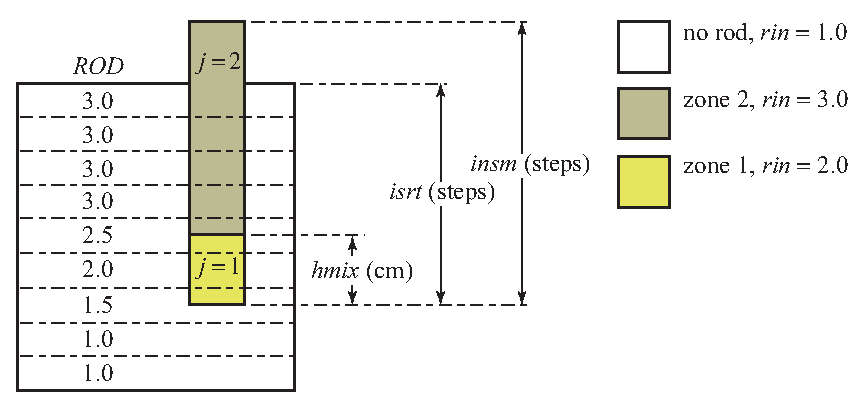
\includegraphics[scale=0.8]{Figures/rod_pwr.eps} 
\caption{Presentation of a partially-inserted 2-part control rod.}\label{fig:rod_pwr}
  \end{center}
\end{figure}

Recommended values are:

\vskip 0.2cm
\begin{tabular}{|c|l|}
\hline
RIN & type of bar \\
\hline
0 & AICG (grey bar, generally out at nominal power) \\
1 ($=$ \dusa{val1}) & rod extracted \\
2 & AICN (black bar, generally out or partly inserted) \\
3 & B4C (black bar, generally out or partly inserted) \\
\hline
\end{tabular}
\vskip 0.2cm

The rod identification number is interpolated over each axial mesh of the fuel map. A local parameter name \dusa{par1} is defined and their distributed values are computed by the {\tt ROD:} module as depicted in Fig.~\ref{fig:rod_pwr}. Local parameters \dusa{par1} are identified as {\sl ROD} in the figure. A local value of {\sl ROD} $=2.5$ corresponds to a mesh of the fuel map containing 50\% of AICN material and 50\% of B4C material.

\noindent

\begin{DataStructure}{Structure \dstr{descrod1}}
$[$ \moc{EDIT} \dusa{iprint} $]$\\
$[$ \moc{PARA} \dusa{par1} \dusa{val1} $]$ \\
$[$ \moc{LINS} \dusa{insm} $]$\\
$[$ \moc{STEP} \dusa{step} $]$\\
$[$ \moc{NRFB} \dusa{nrfb} $]$\\
$[$ \moc{RGRP} \\ 
~~~$\{$ \dusa{ngrp} \dusa{maxmix} \\
~~~~~ ((\dusa{hgrp}(i) \dusa{isrt(i)} \dusa{rin(i,1)} $[[$ \dusa{hmix}(i,j) \dusa{rin(i,j+1)} $]]$), i=1, \dusa{ngrp}, j=1, \dusa{lmix}-1) \\
~~~$|$ \dusa{nrmv} \\
~~~~~ ((\dusa{hgrp}(i) \dusa{isrt(i)}), i=1, \dusa{nrmv}) $\}$ \\
\moc{ENDRGRP} $]$\\
$[$ \moc{RMAP} \dusa{nass} \\
~~~ ((\dusa{hrod}(i,j)), i=1, \dusa{lx}, j=1,ly ) \\
\moc{ENDRMAP} $]$ \\
\moc{;}
\end{DataStructure}

\goodbreak

\noindent where

\begin{ListeDeDescription}{mmmmmmmm}

\item[\moc{EDIT}] keyword used to set \dusa{iprint}.

\item[\dusa{iprint}] integer index used to control the printing on screen:
 = 0 for no print; = 1 for minimum printing (default value); larger values
produce increasing amounts of output.

\item[\moc{PARA}] keyword used to indicate that the name of the record to be
contained the rod field will follow.

\item[\dusa{par1}] name of the rod record and local parameter to be created. This name must correspond to the rod name of the {\sc saphyb} or {\sc multicompo} object.

\item[\dusa{val1}] real value of the 3-D rod field \dusa{par1}. This value enables to initialise the field to a uniform value, corresponding to a core with no rod inserted.

\item[\moc{LINS}] keyword used to indicate the maximum number of insertion steps 
for all rods.

\item[\dusa{insm}] integer value of maximum rod insertion step.

\item[\moc{STEP}] keyword used to indicate the length of one rod step.

\item[\dusa{step}] real value of rod step length (in cm).

\item[\moc{NRFB}] keyword used to indicate the number of bottom-reflective meshes
in the core.

\item[\dusa{nrfb}] integer value of bottom-reflective meshes in the core.

\item[\moc{RGRP}] keyword used to define all rod groups present in the core.

\item[\dusa{ngrp}] integer value of the number of rod groups present in the core.

\item[\dusa{maxmix}] integer value of the maximum number of rod zones (for hybrid 
rods with many materials).

\item[\dusa{nrmv}] integer value of the number of rod groups that rod insertion is modified.

\item[\dusa{hgrp}] \texttt{character*3} identification value for the rod group $i$.

\item[\dusa{isrt}] integer value for the number of inserted steps for the rod group $i$.

\item[\dusa{rin}] real value for the rod identification number (RIN) considered from the {\sc saphyb} or {\sc multicompo} object.

\item[\dusa{hmix}] real value for the height (in cm) of the RIN considered.
If only one RIN is used to define the rod, \dusa{hmix} is not defined. If two or more RIN are used for one rod, 
the values of the lower rod sections with $1\le j < \dusa{lmix}$ should be defined, as depicted in Fig.~\ref{fig:rod_pwr}.

\item[\dusa{lmix}] integer value for the number of \dusa{rin} for each rod group.

\item[\moc{ENDRGRP}] keyword used to indicate the end of rod groups definition.

\item[\moc{RMAP}] keyword used to define the position of each rod group inside the core.

\item[\dusa{nass}] integer value of number of assemblies inside the core.

\item[\dusa{hrod}] \texttt{character*3} identification value for the (i,j) position. Accepted
values are:
\begin{itemize}
\item \moc{|}, \moc{-} or \moc{-|-} for an unrodded assembly,
\item or a \texttt{character*3} identification value referring to the identification value of the rod group.
\end{itemize}

\item[\moc{ENDRMAP}] keyword used to indicate the end of rod group position map.

\end{ListeDeDescription}

\eject

\vskip 1.0cm
\subsection{The \moc{IDET:} module}\label{sect:idet}

\vskip 0.2cm
The \moc{IDET:} module can perform an evaluation of fission chamber response in a PWR by integrating the fission rate over
the detector positions. This module is limited to Cartesian geometry.

\vskip 0.08cm
\noindent
The \moc{IDET:} module specification is:

\begin{DataStructure}{Structure \moc{IDET:}}\label{table:tidet}
\dusa{IDETEC} \moc{:=} \moc{IDET:} $[$ \dusa{IDETEC} $]$ \dusa{TRKNAM} \dusa{FLUNAM} \dusa{LIBNAM} $[$ \dusa{FMAP} $]$ \\
\moc{::} \dstr{descidet}
\end{DataStructure}

\noindent where

\begin{ListeDeDescription}{mmmmmmmm}

\item[\dusa{IDETEC}] {\tt character*12} name of a \dds{idetect} data structure,
({\tt L\_INTDETEC} signature) that will be created or updated by the \moc{IDET:} module.

\item[\dusa{TRKNAM}] {\tt character*12} name of the read-only \dds{tracking} data
structure ({\tt L\_TRACK} signature) containing the finite-element tracking.

\item[\dusa{FLUNAM}] {\tt character*12} name of the read-only \dds{fluxunk} data
structure ({\tt L\_FLUX} signature) containing the finite-element solution.

\item[\dusa{LIBNAM}] {\tt character*12} name of the read-only \dds{macrolib}
data structure ({\tt L\_LIBRARY} signature) that contains the interpolated microscopic
cross sections.

\item[\dusa{FMAP}] \texttt{character*12} name of the read-only  \dds{fmap} data structure
({\tt L\_MAP} signature) containing renumbered mixture indices. This object is optionnal.

\item[\dstr{descidet}] structure describing the input data to the \moc{IDET:} module.

\end{ListeDeDescription}

\subsubsection{Input data to the \moc{IDET:} module}\label{sect:stridet}

\begin{DataStructure}{Structure \dstr{descidet}}
$[$ \moc{EDIT} \dusa{iprint} $]$ \\
$[~\{$ \moc{NOCCOR} $|$ \moc{CCOR} $\}~]$ \\
$[$ \moc{DETNAME} \dusa{dname} $]~[$ \moc{REANAME} \dusa{rname} $]$ \\
\moc{DETECTOR} \\
\hspace{0.3cm} $[[$ \moc{POSITION} $\{$ \dusa{valx} $|$ \moc{INTEG} \dusa{valx1} \dusa{valx2} $\}~\{$ \dusa{valy} $|$ \moc{INTEG} \dusa{valy1} \dusa{valy2} $\}$ \\
\hspace{2.02cm} $[~\{$ \dusa{valz} $|$ \moc{INTEG} \dusa{valz1} \dusa{valz2} $\}~]~]]$ \\
\moc{ENDD} \\
;
\end{DataStructure}

\noindent where
\begin{ListeDeDescription}{mmmmmmmm}

\item[\moc{EDIT}] keyword used to set \dusa{iprint}.

\item[\dusa{iprint}] integer index used to control the printing on screen:
 = 0 for no print; = 1 for minimum printing (default value); =2 for more printouts.

\item[\moc{NOCCOR}] keyword used to desactivate {\sl corner flux correction} with 2D/3D nodal methods.

\item[\moc{CCOR}] keyword used to activate {\sl corner flux correction} with 2D/3D nodal methods (default option).

\item[\moc{DETNAME}] keyword used to set \dusa{dname}, the alias name of the isotope used as detector. By default, \dusa{dname}$=${\tt U235} is used.

\item[\dusa{dname}] character*12 alias name of the isotope used as detector.

\item[\moc{REANAME}] keyword used to set \dusa{rname}, the name of the nuclear reaction used as detector. By default, \dusa{rname}$=${\tt NFTOT} is used.

\item[\dusa{rname}] character*12 name of the nuclear reaction used as detector.

\item[\moc{POSITION}] keyword defining the position of a single detector.

\item[\moc{INTEG}] keyword indicating that the detector reading will be averaged between two Cartesian positions.

\item[\dusa{valx}] position (real number) of the detector along $X$ axis.

\item[\dusa{valx1}] starting position (real number) of the detector along $X$ axis.

\item[\dusa{valx2}] ending position (real number) of the detector along $X$ axis. We must have \dusa{valx1}$<$\dusa{valx2}.
 
\item[\dusa{valy}] position (real number) of the detector along $Y$ axis.

\item[\dusa{valy1}] starting position (real number) of the detector along $Y$ axis.

\item[\dusa{valy2}] ending position (real number) of the detector along $Y$ axis. We must have \dusa{valy1}$<$\dusa{valy2}.
 
\item[\dusa{valz}] position (real number) of the detector along $Z$ axis. Detector position along $Z$ axis is given only for 3D geometries.

\item[\dusa{valz1}] starting position (real number) of the detector along $Z$ axis.

\item[\dusa{valz2}] ending position (real number) of the detector along $Z$ axis. We must have \dusa{valz1}$<$\dusa{valz2}.

\end{ListeDeDescription}
\clearpage


\section{CROSS-SECTION INTERPOLATION MODULES}\label{sect:modesc2}

\subsection{The \moc{CRE:} module}\label{sect:cre}

The \moc{CRE:} module is used for the recovering and interpolation of nuclear
properties from one or many \dds{compo} objects, originated from the transport
calculations using lattice code DRAGON. A resulting \dds{macrolib}
will be created (or updated) by the \moc{CRE:} module, it will contain the nuclear
properties of some selected reactor materials.\\

\noindent
Two types of \dds{macrolib} can be constructed using the \moc{CRE:} module:

\begin{itemize}

\item  A \dds{macrolib} that will be constructed for the few reactor materials,
namely for the devices and/or reflector properties. It can also be created for
the few fuel regions defined in the reactor core. This \dds{macrolib} is
permitted to be updated for the new properties in the subsequent calls to the
\moc{CRE:} module.
\item A fuel-map \dds{macrolib} that will be constructed over the fuel lattice
only. This \dds{macrolib} will contain a set of interpolated fuel properties with
respect to the burnup distribution over the fuel lattice and according to the
interpolation option defined in the \dds{fmap} object. The total number of mixtures
in the resulting \dds{macrolib} will equal to the total number of fuel bundles.
\end{itemize}

\noindent
Note that the \moc{CRE:} module can be used only with the mono-parameter
\dds{compo} objects and the nuclear properties can be interpolated only with
respect to the burnup data. In case of the \dds{macrolib} construction from a
multi-parameter database, the \moc{NCR:} module should be used instead.
In this case, the interpolation of nuclear properties can be made with respect
to global and local parameters, if they were previously specified in the fuel-map
(see \Sect{resiniaram}).\\

\noindent
The \moc{CRE:} module specifications are:

\begin{DataStructure}{Structure \moc{CRE:}}
$\{$ \dusa{MACRO} \moc{:=} \moc{CRE:} $[$ \dusa{MACRO} $]$
$[[$ \dusa{CPO} $]]$  \moc{::} \dstr{desccre1} $|$ \\
~~~\dusa{MACFL} \moc{:=} \moc{CRE:} $[[$ \dusa{CPO} $]]$
\dusa{FMAP} \moc{::} \dstr{desccre2} $\}$
\end{DataStructure}

\noindent where
\begin{ListeDeDescription}{mmmmmmmm}

\item[\dusa{MACRO}] \texttt{character*12} name of the \dds{macrolib}
object to be created or updated for the few reactor material properties.
Note that if \dusa{MACRO} appears on the RHS, the information previously
stored in \dusa{MACRO} is kept.

\item[\dusa{CPO}] \texttt{character*12} name of the \dds{compo} object
containing the mono-parameter database from transport calculations.

\item[\dusa{MACFL}] \texttt{character*12} name of the fuel-map \dds{macrolib}
that will be created only for the fuel properties over the fuel lattice.

\item[\dusa{FMAP}] \texttt{character*12} name of the \dds{fmap} object
containing the fuel-map specification and burnup informations.

\item[\dstr{desccre1}] structure describing the input data to the \moc{CRE:}
module when the \dds{fmap} object is not specified.

\item[\dstr{desccre2}] structure describing the input data to the \moc{CRE:}
module for the fuel-map \dds{macrolib} construction.

\end{ListeDeDescription}

\subsubsection{Input data for the \moc{CRE:} module}

\begin{DataStructure}{Structure \dstr{desccre1}}
$[$ \moc{EDIT} \dusa{iprint} $]$ \\
$[$ \moc{NMIX} \dusa{nmix} $]$ \\
\moc{READ} $[[$ \moc{COMPO} \dusa{CPO} \dstr{descdata1} $]]$ \\
;
\end{DataStructure}

\begin{DataStructure}{Structure \dstr{desccre2}}
$[$ \moc{EDIT} \dusa{iprint} $]$ \\
\moc{READ} $[[$ \moc{TABLE} \dusa{CPO} \dstr{descdata2} $]]$ \\
;
\end{DataStructure}

\goodbreak
\noindent where
\begin{ListeDeDescription}{mmmmmmmm}

\item[\moc{EDIT}] keyword used to set \dusa{iprint}.

\item[\dusa{iprint}] integer index used to control the printing of
information on screen: = 0 for no print; = 1 for minimum printing;
larger values will produce increasing amounts of output.

\item[\moc{NMIX}] keyword used to define the number of material
mixtures \dusa{nmix}. This data must be given only if \dusa{MACRO}
is created and the \dds{fmap} object is not specified.

\item[\dusa{nmix}] integer maximum number of reactor material mixtures,
as defined in the reactor geometry.

\item[\moc{READ}] keyword used to read the \dds{macrolib} specification
from the input data file.

\item[\moc{COMPO}] keyword used to indicate a simple \dds{macrolib} creation,
i.e. according to the first calling specification when \dds{fmap} object is not specified.

\item[\moc{TABLE}] keyword used to indicate a fuel-map \dds{macrolib} creation,
i.e. according to the second calling specification with \dds{fmap} object specified.

\item[\dusa{CPO}] \texttt{character*12} name of the selected \dds{compo} object.
This name must appear in the calling specification to the \moc{CRE:} module.

\item[\dstr{descdata1}] structure containing the interpolation specification if
\moc{COMPO} is the selected option.

\item[\dstr{descdata2}] structure containing the interpolation specification if
\moc{TABLE} is the selected option.

\end{ListeDeDescription}

\begin{DataStructure}{Structure \dstr{descdata1}}
$[[$ \moc{MIX} \dusa{mix} \dusa{NAMDIR} $~[$ \moc{DERIV} $]~[$ \moc{UPS} $]$ \\
~~~~$[$ $\{$ \moc{I-BURNUP} \dusa{burn} $|$ \moc{T-BURNUP} \dusa{burn0} \dusa{burn1} $\}$ $]$ \\
~~~~$[$ \moc{MICRO} $\{$ $[[$ \dusa{HISO} $\{$ \dusa{conc} $|$ \moc{*} $\}$ $]]~|$ \moc{ALL} $\}$ $]$ \\
\moc{ENDMIX} $]]$
\end{DataStructure}

\begin{DataStructure}{Structure \dstr{descdata2}}
$[[$ \moc{MIX} \dusa{mix} \dusa{NAMDIR} $~[$ \moc{DERIV} $]~[$ \moc{UPS} $]$ \\
~~~~$[~\{$~\moc{TIMAV-BURN} $|$ \moc{INST-BURN} $|$ \moc{AVG-EX-BURN}~\dusa{ivarty}~$\}~]$ \\
~~~~$[$ \moc{MICRO} $\{$ $[[$ \dusa{HISO} $\{$ \dusa{conc} $|$ \moc{*} $\}$ $]]~|$ \moc{ALL} $\}$ $]$ \\
\moc{ENDMIX} $]]$
\end{DataStructure}

\noindent where
\begin{ListeDeDescription}{mmmmmmmm}

\item[\moc{MIX}] keyword used to set the material mixture \dusa{mix}.

\item[\dusa{mix}] integer identifier for the material mixture that will be
included in the \dds{macrolib}. The maximum number of identifiers
permitted is \dusa{nmix} and the maximum value that \dusa{mix} may
have is \dusa{nmix}. Note that if \moc{TABLE} is the selected option,
then \dusa{mix} identifies the fuel type as defined in the reactor geometry.

\item[\dusa{NAMDIR}] \texttt{character*12} directory name in the
\dusa{CPO} object from which the nuclear properties for material
mixture \dusa{mix} are to be recovered.

\item[\moc{DERIV}] keyword used to compute the derivative of the
\dds{macrolib} information with respect to \dusa{burn} or \dusa{burn1}
value. By default, the \dds{macrolib} information is not differentiated.

\item[\moc{UPS}] keyword used to compute properties with no
up-scattering contribution.

\item[\moc{TIMAV-BURN}] keyword used to compute time-averaged cross-section information.
This option is available {\sl only if} \moc{TABLE} is the selected option.
By default, the type of calculation (\moc{TIMAV-BURN} or \moc{INST-BURN})
is recovered from the \dusa{FMAP} object.

\item[\moc{INST-BURN}] keyword used to compute cross-section information
at specific bundle burnups. This option is available {\sl only if} \moc{TABLE} is the selected option.
By default, the type of calculation (\moc{TIMAV-BURN} or \moc{INST-BURN})
is recovered from the \dusa{FMAP} object.

\item[\moc{AVG-EX-BURN}] keyword used to compute the derivatives of cross-section
information relative to the exit burnup of a single combustion zone. The derivatives are
computed using Eq.~(3.3) of Ref.~\citen{chambon}, written as
$$
{\partial \bar\Sigma_x\over \partial B_j^{\rm e}}={1\over B_j^{\rm e}\, (B_{j,k}^{\rm eoc}-B_{j,k}^{\rm boc})}
\left[- \int_{B_{j,k}^{\rm boc}}^{B_{j,k}^{\rm eoc}}dB \, \Sigma_x(B)+B_{j,k}^{\rm eoc}\, \Sigma_x(B_{j,k}^{\rm eoc})-B_{j,k}^{\rm boc}\, \Sigma_x(B_{j,k}^{\rm boc})\right]
$$

\noindent where $B_{j,k}^{\rm boc}$, $B_{j,k}^{\rm eoc}$, and $B_j^{\rm e}$ are the beginning of cycle burnup of bundle $\{j,k\}$, end of cycle burnup of bundle $\{j,k\}$ and exit burnup of channel $j$. This option is available {\sl only if} \moc{TABLE} is the selected option.

\item[\dusa{ivarty}] index of the combustion zone for differentiation of cross-section information.

\item[\moc{I-BURNUP}] keyword used to perform a single interpolation
and to set the burnup interpolation value \dusa{burn}.

\item[\dusa{burn}] real interpolation value of the burnup, given in
MW$\cdot$day per tonne of initial heavy elements.

\item[\moc{T-BURNUP}] keyword used to perform a time-average
\dds{macrolib} evaluation between the burnup values \dusa{burn0}
and \dusa{burn1}.

\item[\dusa{burn0}] real initial value of the burnup, given in MW$\cdot$day
per tonne of initial heavy elements.

\item[\dusa{burn1}] real final value of the burnup, given in MW$\cdot$day
per tonne of initial heavy elements.

\item[\moc{MICRO}] keyword used to set the number densities of the extracted
isotopes present in the \dds{compo} linked list or \dds{xsm} file. By default, the
extracted isotopes are not added to the resulting \dds{macrolib}.

\item[\dusa{HISO}] \texttt{character*12} name of an extracted isotope.

\item[\dusa{conc}] user-defined real number density of the extracted isotope,
given in $10^{24}$ particles per ${\rm cm}^3$.

\item[\moc{*}] keyword used to indicate that the number density for the
isotope \dusa{HISO} will be recovered from the \dds{compo} object.

\item[\moc{ALL}] keyword used to indicate that all the number densities are to
be recovered from the \dds{compo} object.

\item[\moc{ENDMIX}] keyword used to indicate the end of data specification
for the material mixture \dusa{mix}.

\end{ListeDeDescription}
\clearpage

\vskip 1.0cm
\subsection{The {\tt NCR:} module}\label{sect:NCRData}

This component of DONJON is dedicated to the interpolation of {\sc microlib} and
{\sc macrolib} data from a {\sc multicompo} object, the reactor database produced by {\tt COMPO:}.
A set of {\sl global} and/or {\sl local parameters} are defined for each material mixture and
used as multi-dimensional interpolation variables.

\vskip 0.02cm

The calling specifications are:

\begin{DataStructure}{Structure \dstr{NCR:}}
\dusa{MLIB}~\moc{:=}~\moc{NCR:}~$[~\{$~\dusa{MLIB} $|$ \dusa{MLIB2}~$\}~]$ \dusa{CPONAM1} $[[$~\dusa{CPONAM2}~$]]~[$~\dusa{MAPFL}~$]$~\moc{::}~\dstr{ncr\_data} \\
\end{DataStructure}

\noindent where
\begin{ListeDeDescription}{mmmmmmm}

\item[\dusa{MLIB}] {\tt character*12} name of a {\sc microlib} (type {\tt L\_LIBRARY}) or {\sc macrolib} (type {\tt L\_MACROLIB}) containing the interpolated
data. If this object also appears on the RHS of structure \dstr{NCR:}, it is open in modification mode and updated.

\item[\dusa{MLIB2}] {\tt character*12} name of an optional {\sc microlib} object whose content is copied on \dusa{MLIB}.

\item[\dusa{CPONAM1}] {\tt character*12} name of the {\sc lcm} object containing the
{\sc multicompo} data structure ({\tt L\_MULTICOMPO} signature).

\item[\dusa{CPONAM2}] {\tt character*12} name of an additional {\sc lcm} object containing an auxiliary
{\sc multicompo} data structure ({\tt L\_MULTICOMPO} signature). This object is optional.

\item[\dusa{MAPFL}] {\tt character*12} name of the {\sc map} object containing fuel regions description, global and local parameter
information (burnup, fuel/coolant temperatures, coolant density, etc). Keyword \moc{TABLE} is expected in \dstr{ncr\_data}.

\item[\dusa{ncr\_data}] input data structure containing interpolation information (see \Sect{descncr}).

\end{ListeDeDescription}

\subsubsection{Interpolation data input for module {\tt NCR:}}\label{sect:descncr}

\vskip -0.5cm

\begin{DataStructure}{Structure \dstr{ncr\_data}}
$[$~\moc{EDIT} \dusa{iprint}~$]$ \\
$[$~\moc{ALLX} \dusa{nbfuel}~$]~[$~\moc{RES} $]~[$~\moc{PURE} $]$ \\
$[~\{$~\moc{MACRO}~$|$~\moc{MICRO}~$\}~]~[~\{$~\moc{LINEAR}~$|$~\moc{CUBIC}~$\}~]~[$~\moc{LEAK}~\dusa{b2}~$]$ \\
$[$~\moc{NMIX} \dusa{nmixt}~$]$ \\
$\{~[[$~\moc{COMPO} \dusa{CPONAM} \dusa{NAMDIR} \dstr{descintf}~$]]$ \\ 
$~|~[[$~\moc{TABLE} \dusa{CPONAM} \dusa{NAMDIR} $[$ \dusa{namburn} $[$ \dusa{naval} $]~]$ \dstr{descintf}~$]]~\}$ \\
{\tt ;}
\end{DataStructure}

\noindent where
\begin{ListeDeDescription}{mmmmmmmm}

\item[\moc{EDIT}] keyword used to set \dusa{iprint}.

\item[\dusa{iprint}] index used to control the printing in module {\tt NCR:}. =0 for no print; =1 for minimum printing (default value).

\item[\moc{ALLX}] keyword used to register the region number of each isotope before merging. This option is useful if the same keyword has been specified in \moc{EDI:} and \moc{COMPO:} before.

\item[\dusa{nbfuel}] number of fuel rings used for micro-depletion calculations.

\item[\moc{RES}] keyword indicating that the interpolation is done only for the microscopic cross sections and not for the isotopic densities. In this case, a RHS {\sc microlib} must be defined and the number densities are recovered from it. This option is useful for micro-depletion applications. {\bf Important note:} It is possible to force interpolation of some isotopic densities with \moc{RES} option if these
isotopes are explicitely specified with a ``\moc{*}'' flag after \moc{MICRO} keyword in \dusa{descintf} input data structure (see \Sect{descintf}).

\item[\moc{PURE}] keyword indicating that the interpolation is a pure linear combination of terp factors. The fission spectra are {\sl not}
renormalized. By default, non-linear effects are produced by renormalization operations.

\item[\moc{MACRO}] keyword indicating that \dusa{MLIB} is a {\sc macrolib}.

\item[\moc{MICRO}] keyword indicating that \dusa{MLIB} is a {\sc microlib} (default option). Object \dusa{MLIB} contains an embedded {\sc macrolib}, but the CPU time required to obtain it is longer.

\item[\moc{LINEAR}] keyword indicating that interpolation of the {\sc multicompo} uses linear Lagrange polynomials (default option).

\item[\moc{CUBIC}] keyword indicating that interpolation of the {\sc multicompo} uses the Ceschino method
with cubic Hermite polynomials, as presented in Ref.~\citen{Intech2011}.

\item[\moc{LEAK}] keyword used to introduce leakage in the embedded {\sc macrolib}. This option should only be used for non-regression tests.

\item[\dusa{b2}] the imposed buckling corresponding to the leakage.

\item[\moc{NMIX}] keyword used to define the maximum number of material mixtures. This information is required  only if \dusa{MLIB} is created.

\item[\dusa{nmixt}] the maximum number of mixtures (a mixture is characterized by a distinct set of 
macroscopic cross sections) the {\sc macrolib} may contain. The default value is \dusa{nmixt} $=0$ or the value recovered from \dusa{MLIB} if it appears on
the RHS of structure \dstr{NCR:}.

\item[\moc{COMPO}] keyword used to set \dusa{CPONAM} and to define each global and local parameter.

\item[\moc{TABLE}] keyword used to set \dusa{CPONAM} and to recover some global and local parameter from a {\sc map} object named \dusa{MAPFL}.

\item[\dusa{CPONAM}] {\tt character*12} name of the {\sc lcm} object containing the
{\sc multicompo} data structure where the interpolation is performed. This name must be set in the RHS of structure \dstr{NCR:}.

\item[\dusa{NAMDIR}] access the {\sc multicompo} structure of \dusa{CPONAM} from the sub-directory named \dusa{NAMDIR}.
This value must be set equal to {\tt 'default'} if not previously defined by a {\tt STEP UP} keyword in module {\tt COMPO}.

\item[\dusa{namburn}] {\tt character*12} name of the parameter for burnup (or irradiation) in the sub-directory named \dusa{NAMDIR}.
This value is defined if option \moc{TABLE} is set {\sl and} if burnup (or irradiation) is to be considered as parameter.

\item[\dusa{naval}] {\tt character*4} identification name corresponding to the basic naval-coordinate position of the assembly where burnups are recovered. The axial burnup distribution of this assembly is
used for interpolation. {\tt SIM} option should be set in module {\tt RESINI:} (see Sect.~\ref{sect:resinimain}). This option is useful to interpolate reflector properties as a function of the
neighbour fuel assembly burnup. By default, burnup values of the interpolated fuel assembly are used.

\item[\dusa{descintf}] input data structure containing interpolation information relative to the {\sc multicompo} data structure named \dusa{CPONAM} (see \Sect{descintf}).

\end{ListeDeDescription}

\subsubsection{Defining local and global parameters}\label{sect:descintf}

\vskip -0.5cm

If a {\sc map} object is defined on the RHS of structure \dstr{NCR:}, and if the \moc{TABLE} keyword is set, some information required to set the interpolation points is found in this object. In this case, the {\tt NCR:} operator search the {\sc multicompo} object for global or local parameters  having an arbitrary name specified in the {\sc map} object or set directly in  this module. Note that any parameter's value set directly in this module prevails on a value stored in the \dusa{MAPFL} object.

Each instance of \dusa{descintf} is a data structure specified as

\begin{DataStructure}{Structure \dstr{descintf}}
$[[$~\moc{MIX} \dusa{imix}~$[~\{$~\moc{FROM}~\dusa{imixold}~$|$~\moc{USE}~$\}~]$ \\
~~~~~~$[~\{$~\moc{TIMAV-BURN} $|$ \moc{INST-BURN} $|$ \moc{AVG-EX-BURN}~\dusa{ivarty}~$\}~]$ \\
~~~~~~$[[~\{$~\moc{SET} $|$ \moc{DELTA} $|$ \moc{ADD}~$\}~\}~[~\{$ \moc{LINEAR} $|$ \moc{CUBIC}~$\}~]$ \dusa{PARKEY} $\{$~\dusa{val1} $|$ \moc{MAP}~$\}~[~\{$~\dusa{val2} $|$ \moc{MAP}~$\}~]$ \\
~~~~~~~~~~~~$[$~\moc{REF} $[[$~\dusa{PARKEY}~$\{$~\dusa{valref} $|$ \moc{SAMEASREF}~$\}$~$]]$~\moc{ENDREF}~$]~]]$  \\
~~~~~~$[$~\moc{MICRO}~$\{$~\moc{ALL} $|$ \moc{ONLY}~$\}~[[$~\dusa{HISO} $\{$ \dusa{conc} $|$ \moc{*} $\}~]]~]$ \\
\moc{ENDMIX}~$]]$
\end{DataStructure}

\noindent where
\begin{ListeDeDescription}{mmmmmmmm}

\item[\moc{MIX}] keyword used to set \dusa{imix}. Discontinuity factor information present in the Multicompo is interpolated as mixture~1 values.

\item[\dusa{imix}] index of the mixture that is to be created in the {\sc microlib} and {\sc macrolib}.

\item[\moc{FROM}] keyword used to set the index of the mixture in the {\sc multicompo} object.

\item[\dusa{imixold}] index of the mixture that is recovered in the {\sc multicompo} object. By default, \dusa{imixold}$=1$.

\item[\moc{USE}] keyword used to set the index of the mixture in the {\sc multicompo} object equal to \dusa{imix}.

\item[\moc{TIMAV-BURN}] keyword used to compute time-averaged cross-section information. This option is available {\sl only if} a \dusa{MAPFL} object is set.
By default, the type of calculation (\moc{TIMAV-BURN} or \moc{INST-BURN}) is recovered from the \dusa{MAPFL} object.

\item[\moc{INST-BURN}] keyword used to compute cross-section information at specific bundle burnups. This option is available {\sl only if} a \dusa{MAPFL} object is set.
By default, the type of calculation (\moc{TIMAV-BURN} or \moc{INST-BURN}) is recovered from the \dusa{MAPFL} object.

\item[\moc{AVG-EX-BURN}] keyword used to compute the derivatives of cross-section information relative to the exit burnup of a single combustion zone. The derivatives are computed using Eq.~(3.3) of Ref.~\citen{chambon}, written as
$$
{\partial \bar\Sigma_x\over \partial B_j^{\rm e}}={1\over B_j^{\rm e}\, (B_{j,k}^{\rm eoc}-B_{j,k}^{\rm boc})}
\left[- \int_{B_{j,k}^{\rm boc}}^{B_{j,k}^{\rm eoc}}dB \, \Sigma_x(B)+B_{j,k}^{\rm eoc}\, \Sigma_x(B_{j,k}^{\rm eoc})-B_{j,k}^{\rm boc}\, \Sigma_x(B_{j,k}^{\rm boc})\right]
$$

\noindent where $B_{j,k}^{\rm boc}$, $B_{j,k}^{\rm eoc}$, and $B_j^{\rm e}$ are the beginning of cycle burnup of bundle $\{j,k\}$, end of cycle burnup of bundle $\{j,k\}$ and exit burnup of channel $j$. This option is available {\sl only if} a \dusa{MAPFL} object is set.
By default, the type of calculation (\moc{TIMAV-BURN} or \moc{INST-BURN}) is recovered from the \dusa{MAPFL} object.

\item[\dusa{ivarty}] index of the combustion zone for differentiation of cross-section information.

\item[\moc{SET}] keyword used to indicate a simple interpolation at \dusa{val1} or an averaging between \dusa{val1} and \dusa{val2}. The result $\sigma_{\rm ref}$ is also used as the reference value when the \moc{ADD} is used. Note: see at the ending note of this section for a detailed description and examples.

\item[\moc{DELTA}] keyword used to indicate a delta-sigma calculation between \dusa{val2} and \dusa{val1}
(i.e., $\Delta\sigma_{\rm ref}=\sigma_{\rm val2}-\sigma_{\rm val1}$ is computed). This keyword can be used only once in each mixture data block (initiated
with a \moc{MIX} keyword).  Note: see at the ending note of this section for a detailed description and examples.

\item[\moc{ADD}] keyword used to indicate a delta-sigma calculation between \dusa{val2} and \dusa{val1} is added to the reference value
(i.e., $\Delta\sigma=\sigma_{\rm val2}-\sigma_{\rm val1}$ is used as contribution, $\sigma_{\rm ref}+\Delta\sigma$ or $\Delta\sigma_{\rm ref}+\Delta\sigma$ is returned). Note: see at the ending note of this section for a detailed description and examples.

\item[\moc{LINEAR}] keyword indicating that interpolation of the {\sc multicompo} for parameter \dusa{PARKEY} uses linear Lagrange
polynomials. It is possible to set different interpolation modes to different parameters. By default, the interpolation mode is set in Sect.~\ref{sect:descncr}.

\item[\moc{CUBIC}] keyword indicating that interpolation of the {\sc multicompo} for parameter \dusa{PARKEY} uses the Ceschino method
with cubic Hermite polynomials, as presented in Ref.~\citen{Intech2011}. By default, the interpolation mode is set in Sect.~\ref{sect:descncr}.

\item[\dusa{PARKEY}] {\tt character*12} user-defined keyword associated to a global
or local parameter to be set.

\item[\dusa{val1}] value of a global or local parameter used to interpolate.  \dusa{val1} is the initial value of this parameter in case an average is required. \dusa{val1} can be an integer, real or string value.

\item[\dusa{val2}] value of the final global or local parameter. By default, a simple interpolation is performed, so that \dusa{val2}$=$\dusa{val1}. \dusa{val2} is always a real value with \dusa{val2}$\ge$\dusa{val1}.

\item[\moc{MAP}] keyword used to indicate that the value of parameter \dusa{val1} or the second value for the $\Delta\sigma$ calculation is
recovered from \dusa{MAPFL}, i.e. the {\sc map} object containing fuel regions description.

\item[\moc{REF}] keyword only available together with the \moc{ADD} option. It is used to set all the other variable values when a $\Delta$ contribution is performed for one variable.  

\item[\dusa{valref}] value of the reference parameter, when it is directly given by the user. Note that there is no default value.

\item[\moc{SAMEASREF}] keyword used to specify that the reference value will be the same as in the refence case, i.e. for the $\sigma_{\rm ref}$ computation.

\item[\moc{ENDREF}] keyword only available together with the \moc{ADD} option. It is used to specify that all the other variable values which are required are given.  

\item[\moc{MICRO}] keyword used to set the number densities of some isotopes present in the {\sc multicompo} object. The data statement ``\moc{MICRO} \moc{ALL}" is used by default.

\item[\moc{ALL}] keyword to indicate that all the isotopes present in the  {\sc multicompo} object will be used in the {\sc microlib} and {\sc macrolib} objects. Concentrations of these isotopes will be recovered from the {\sc multicompo} object
or set using the ``\dusa{HISO} \dusa{conc}" data statement.

\item[\moc{ONLY}] keyword to indicate that only the isotopes set using the ``\dusa{HISO} \dusa{conc}" data statement will be used in the {\sc microlib} and {\sc macrolib} objects.

\item[\dusa{HISO}] {\tt character*8} name of an isotope.

\item[\dusa{conc}] user-defined value of the number density (in $10^{24}$ particles per ${\rm cm}^3$) of the isotope.

\item[\moc{*}] the value of the number density for isotope \dusa{HISO} is recovered from the {\sc multicompo} object.

\item[\moc{ENDMIX}] end of specification keyword for the material mixture.

\end{ListeDeDescription}


\subsubsection{Interpolation in the parameter grid}


The following example corresponds to a delta-sigma computation in mixture 1 corresponding to a perturbation. Note that in this case, the \moc{MACROLIB} object  may content negative cross-section. 
\begin{verbatim}
MACROLIB := NCR: CPO ::
   EDIT 40 NMIX 1 MACRO COMPO CPO default
   MIX 1  !(* delta sigma contribution *)
          SET 'CELL' '3D'
          DELTA 'PITCH' 0.0 1.0
   ENDMIX
;
\end{verbatim}

When the number of parameters used for the interpolation is increased, all the lattice computations corresponding to all the combinations of parameters may not be done for computation time reasons. In this case, some approximations may be required. The choice for the \moc{SET}, \moc{DELTA} and \moc{ADD} is then dependent of the structure of the database (i.e. how the database grid of possibilities is filled). When a {\sc map} object containing fuel regions description is used, the problem become even more complex, because values have to be automatically changed for all bundles. In order to clarify all the different possibilities and limitations dependently of the database structure, we will use a 3 parameter case. The paramaters are referenced by 'A', 'B' and 'C'. But before we explain the different cases, we want to remind that the interpolation factors are computed on each axis seperatly.

The first case corresponds to a complete grid, represented by a gray paralepiped on Fig. \ref{figNCRGRIDINS} and \ref{figNCRGRIDTA}. The
figure \ref{figNCRGRIDINS} shows that the interpolated value in point $V$ can be obtained directly without {\sc map} object. For time-average (TA) computation, lets assume that the parameter 'B' represents the burnup (and keep this convention for other database structure also). In this case the figure \ref{figNCRGRIDTA} shows also that the direct interpolation can be done to compute an average value between the points $V'$ and $V$. Note that the TA burnups are stored in the {\sc map} object, and are then recovered automatically.

The second case corresponds to a partial grid where all the lattice computations have been perfomed for several pairs of parameters, which are represented as the gray rectangles on Fig. \ref{figNCRPLANEINS} and \ref{figNCRPLANETA}. If we use the notations of Fig. \ref{figNCRPLANEINS} and \ref{figNCRPLANETA}, the best estimate interpolated values, $f$, we can get are given by: \\
$f=f(V)~\approx~f(V_B)+(f(V_{BA})-f(V_B))+(f(V_{BC})-f(V_B))=f(V_{BC})+(f(V_{BA})-f(V_B))=f(V_{BA})+(f(V_{BC})-f(V_B))$ for instataneous\\
$f=f(V',V)~\approx~f(V'_B,V_B)+(f(V'_{BA},V_{BA})-f(V'_B,V_B))+(f(V'_{BC},V_{BC})-f(V'_B,V_B))=f(V'_{BC},V_{BC})+(f(V'_{BA},V_{BA})-f(V'_B,V_B))=f(V'_{BA},V_{BA})+(f(V'_{BC},V_{BC})-f(V'_B,V_B))$ for TA\\
~~~~where $f(.,.)$ represents the average value between two points.

The third case corresponds to a minimal grid, where the lattice computations have been perfomed only for one parameter variation at a time. In this case, the grid is represented by the thick gray lines on the axis on Fig. \ref{figNCRAXEINS} and \ref{figNCRAXETA}. If we use the notations of Fig. \ref{figNCRAXEINS} and \ref{figNCRAXETA}, the best estimate interpolated values, $f$, we can get are given by: \\
$f=f(V)~\approx~f(V_0)+(f(V_A)-f(V_0))+(f(V_B)-f(V_0))+(f(V_C)-f(V_0))=f(V_B)+(f(V_A)-f(V_0))+(f(V_C)-f(V_0))$ for instataneous\\
$f=f(V',V)~\approx~f(V'_B,V_B)+(f(V_A)-f(V_0))+(f(V_C)-f(V_0))$ for TA\\
Note that the reference point ($V_0$ in the example) does not have to be the same for all parameters. Database structures such as represented on Fig \ref{figNCRAXEINSbis} can also been used. In this case, we even have two choices for the $\Delta f$ computation on axis 'A'. 

The last case is in fact a mix of cases 2 and 3. The gray rectangle and the gray line on Fig. \ref{figNCRPLAXINS} and \ref{figNCRPLAXTA} reprensent where all the lattice computations have been performed. With the notations used on those figures, one can write that the best estimate interpolated values, $f$, we can get are given by: \\
$f=f(V)~\approx~f(V_B)+(f(V_{BC})-f(V_B))+(f(V_A)-f(V_0))=f(V_{BC})+(f(V_A)-f(V_0))$ for instataneous\\
$f=f(V',V)~\approx~f(V'_B,V_B)+(f(V'_{BC},V_{BC})-f(V'_B,V_B))+(f(V_A)-f(V_0))=f(V'_{BC},V_{BC})+(f(V_A)-f(V_0))$ for TA\\
Note once again that the reference point ($V_0$ in the example) does not have to be the same for all parameters. Database structures such as represented on Fig \ref{figNCRPLAXINSbis} can also been used.
\clearpage

The input files will actually reflect the previous equations. However, they are different if the parameters are stored in a {\sc map} object, \dusa{MAPFL}, or provided directly by the user. For the case of one point interpolation (i.e. instantaneous), the input files will be: \\

\begin{center}
\tablefirsthead{%
\hline
case & all parameters explicitly set & all parameters in {\sc map}\\
\hline}
\tablehead{%
%\hline
%\multicolumn{3}{|l|}{\small\sl continued from previous page}\\
\hline
case & all parameters explicitly set & all parameters in {\sc map}\\
\hline}
\tabletail{%
\hline
\multicolumn{3}{|r|}{\small\sl continued on next page}\\
\hline}
\tablelasttail{\hline}
\bottomcaption{NCR inputs for instantaneous cases}

\begin{supertabular}{|p{0.1\textwidth}|p{0.4\textwidth}|p{0.4\textwidth}|}
%\begin{tabular}{|p{0.1\textwidth}|p{0.4\textwidth}|p{0.4\textwidth}|}
%\hline
%case & all parameters explicitly set & all parameters in {\sc map}\\
\hline
GRID (Fig. \ref{figNCRGRIDINS}) 
& \begin{verbatim}
MACROLIB := NCR: CPO ::
   NMIX 1 MACRO 
   COMPO CPO default
   MIX 1 
      SET 'A' <<va>>
      SET 'B' <<vb>>
      SET 'C' <<vc>>
   ENDMIX
;
\end{verbatim} 
& \begin{verbatim}
MACROLIB := NCR: CPO FMAP ::
   NMIX 1 MACRO 
   TABLE CPO default 'B' 
   MIX 1 
   ENDMIX
;
\end{verbatim} \\
\hline
PLANE (Fig. \ref{figNCRPLANEINS}) & 
\begin{verbatim}
MACROLIB := NCR: CPO ::
   NMIX 1 MACRO 
   COMPO CPO default
   MIX 1 
      SET 'A' <<va>>
      SET 'B' <<vb>>
      SET 'C' <<vc0>>
      ADD 'C' <<vc0>> <<vc>>
         REF  'A' <<va0>> 
              'B' <<vb>> ENDREF
!or           'B' SAMEASREF ENDREF
   ENDMIX
;
\end{verbatim} &
\begin{verbatim}
MACROLIB := NCR: CPO FMAP ::
   NMIX 1 MACRO 
   TABLE CPO default 'B' 
   MIX 1 
      SET 'C' <<vc0>>
      ADD 'C' <<vc0>> MAP
         REF  'A' <<va0>> 
              'B' SAMEASREF ENDREF
!or   SET 'A' <<va0>>
!or   ADD 'A' <<va0>> MAP
!or      REF  'C' <<vc0>> 
!or           'B' SAMEASREF ENDREF
   ENDMIX
;
\end{verbatim} \\
\hline
%\end{tabular}
%
%\begin{tabular}{|p{0.1\textwidth}|p{0.4\textwidth}|p{0.4\textwidth}|}
%\hline
%case & all parameters explicitly set & all parameters in {\sc map}\\
%\hline
AXE (Fig. \ref{figNCRAXEINS}) & 
\begin{verbatim}
MACROLIB := NCR: CPO ::
   NMIX 1 MACRO 
   COMPO CPO default
   MIX 1 
      SET 'A' <<va0>>
      SET 'B' <<vb>>
      SET 'C' <<vc0>>
      ADD 'A' <<va0>> <<va>>
         REF  'C' <<vc0>> 
              'B' <<vb0>> ENDREF
      ADD 'C' <<vc0>> <<vc>>
         REF  'A' <<va0>> 
              'B' <<vb0>> ENDREF
   ENDMIX
;
\end{verbatim} &
\begin{verbatim}
MACROLIB := NCR: CPO FMAP ::
   NMIX 1 MACRO 
   TABLE CPO default 'B' 
   MIX 1 
      SET 'A' <<va0>>
      SET 'C' <<vc0>>
      ADD 'A' <<va0>> MAP
         REF  'C' <<vc0>> 
              'B' <<vb0>> ENDREF
      ADD 'C' <<vc0>> MAP
         REF  'A' <<va0>> 
              'B' <<vb0>> ENDREF
   ENDMIX
;
\end{verbatim} \\
\hline
PLANE + AXE (Fig. \ref{figNCRPLAXINS}) & 
\begin{verbatim}
MACROLIB := NCR: CPO ::
   NMIX 1 MACRO 
   COMPO CPO default
   MIX 1 
      SET 'A' <<va0>>
      SET 'B' <<vb>>
      SET 'C' <<vc>>
      ADD 'A' <<va0>> <<va>>
         REF  'C' <<vc0>> 
              'B' <<vb0>> ENDREF
   ENDMIX
;
\end{verbatim} &
\begin{verbatim}
MACROLIB := NCR: CPO FMAP ::
   NMIX 1 MACRO 
   TABLE CPO default 'B' 
   MIX 1 
      SET 'A' <<va0>>
      ADD 'A' <<va0>> MAP
         REF  'C' <<vc0>> 
              'B' <<vb0>> ENDREF
   ENDMIX
;
\end{verbatim} \\
\hline
%\end{tabular}
\end{supertabular}
\end{center}

For the TA, the burnup variable has no other choice than to be stored in the {\sc map} object, \dusa{MAPFL}. Then the input files will be: \\

\begin{center}
\tablefirsthead{%
\hline
case & only the burnup in {\sc map} & all parameters in {\sc map}\\
\hline}
\tablehead{%
%\hline
%\multicolumn{3}{|l|}{\small\sl continued from previous page}\\
\hline
case & only the burnup in {\sc map} & all param. in {\sc map}\\
\hline}
\tabletail{%
\hline
\multicolumn{3}{|r|}{\small\sl continued on next page}\\
\hline}
\tablelasttail{\hline}
\bottomcaption{NCR inputs for TA cases}

\begin{supertabular}{|p{0.1\textwidth}|p{0.4\textwidth}|p{0.4\textwidth}|}
%\begin{tabular}{p{0.1\textwidth}|p{0.4\textwidth}|p{0.4\textwidth}}
%\hline
%case & only the burnup in {\sc map} & all parameters in {\sc map}\\
\hline
GRID (Fig. \ref{figNCRGRIDTA}) & 
\begin{verbatim}
MACROLIB := NCR: CPO FMAP ::
   NMIX 1 MACRO 
   TABLE CPO default 'B' 
   MIX 1 
      SET 'A' <<va>>
      SET 'C' <<vc>>
   ENDMIX
;
\end{verbatim} &
\begin{verbatim}
MACROLIB := NCR: CPO FMAP ::
   NMIX 1 MACRO 
   TABLE CPO default 'B' 
   MIX 1 
   ENDMIX
;
\end{verbatim} \\
\hline
PLANE (Fig. \ref{figNCRPLANETA}) & 
\begin{verbatim}
MACROLIB := NCR: CPO FMAP ::
   NMIX 1 MACRO 
   TABLE CPO default 'B' 
   MIX 1 
      SET 'A' <<va>>
      SET 'C' <<vc0>>
      ADD 'C' <<vc0>> <<vc>>
         REF  'A' <<va0>> 
              'B' SAMEASREF ENDREF
   ENDMIX
;
\end{verbatim} &
\begin{verbatim}
MACROLIB := NCR: CPO FMAP ::
   NMIX 1 MACRO 
   TABLE CPO default 'B' 
   MIX 1 
      SET 'C' <<vc0>>
      ADD 'C' <<vc0>> MAP
         REF  'A' <<va0>> 
              'B' SAMEASREF ENDREF
!or   SET 'A' <<va0>>
!or   ADD 'A' <<va0>> MAP
!or      REF  'C' <<vc0>> 
!or           'B' SAMEASREF ENDREF
   ENDMIX
;
\end{verbatim} \\
\hline
AXE (Fig. \ref{figNCRAXETA}) & 
\begin{verbatim}
MACROLIB := NCR: CPO FMAP ::
   NMIX 1 MACRO 
   TABLE CPO default 'B' 
   MIX 1 
      SET 'A' <<va0>>
      SET 'C' <<vc0>>
      ADD 'A' <<va0>> <<va>>
         REF  'C' <<vc0>> 
              'B' <<vb0>> ENDREF
      ADD 'C' <<vc0>> <<vc>>
         REF  'A' <<va0>> 
              'B' <<vb0>> ENDREF
   ENDMIX
;
\end{verbatim} &
\begin{verbatim}
MACROLIB := NCR: CPO FMAP ::
   NMIX 1 MACRO 
   TABLE CPO default 'B' 
   MIX 1 
      SET 'A' <<va0>>
      SET 'C' <<vc0>>
      ADD 'A' <<va0>> MAP
         REF  'C' <<vc0>> 
              'B' <<vb0>> ENDREF
      ADD 'C' <<vc0>> MAP
         REF  'A' <<va0>> 
              'B' <<vb0>> ENDREF
   ENDMIX
;
\end{verbatim} \\
\hline
PLANE + AXE (Fig. \ref{figNCRPLAXTA}) & 
\begin{verbatim}
MACROLIB := NCR: CPO FMAP ::
   NMIX 1 MACRO 
   TABLE CPO default 'B' 
   MIX 1 
      SET 'A' <<va0>>
      SET 'C' <<vc>>
      ADD 'A' <<va0>> <<va>>
         REF  'C' <<vc0>> 
              'B' <<vb0>> ENDREF
   ENDMIX
;
\end{verbatim} &
\begin{verbatim}
MACROLIB := NCR: CPO FMAP ::
   NMIX 1 MACRO 
   TABLE CPO default 'B' 
   MIX 1 
      SET 'A' <<va0>>
      ADD 'A' <<va0>> MAP
         REF  'C' <<vc0>> 
              'B' <<vb0>> ENDREF
   ENDMIX
;
\end{verbatim} \\
\hline
%\end{tabular}
\end{supertabular}
\end{center}

\clearpage

The following pictures correspond to the previous different examples:

\begin{multicols}{2}{
\begin{figurehere}
\begin{center}
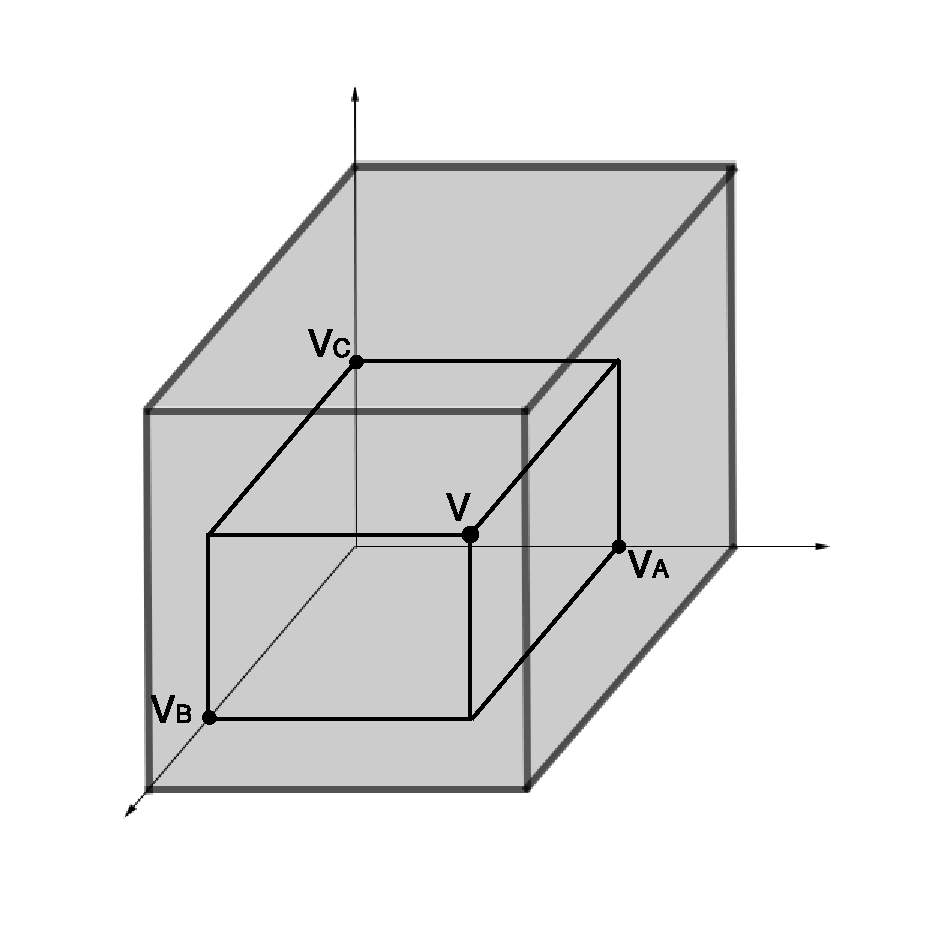
\includegraphics[scale=0.40]{Interpolation-GRID-INS.eps}
\caption{Complete grid, one point case}
\label{figNCRGRIDINS}
\end{center}
\end{figurehere}

\begin{figurehere}
\begin{center}
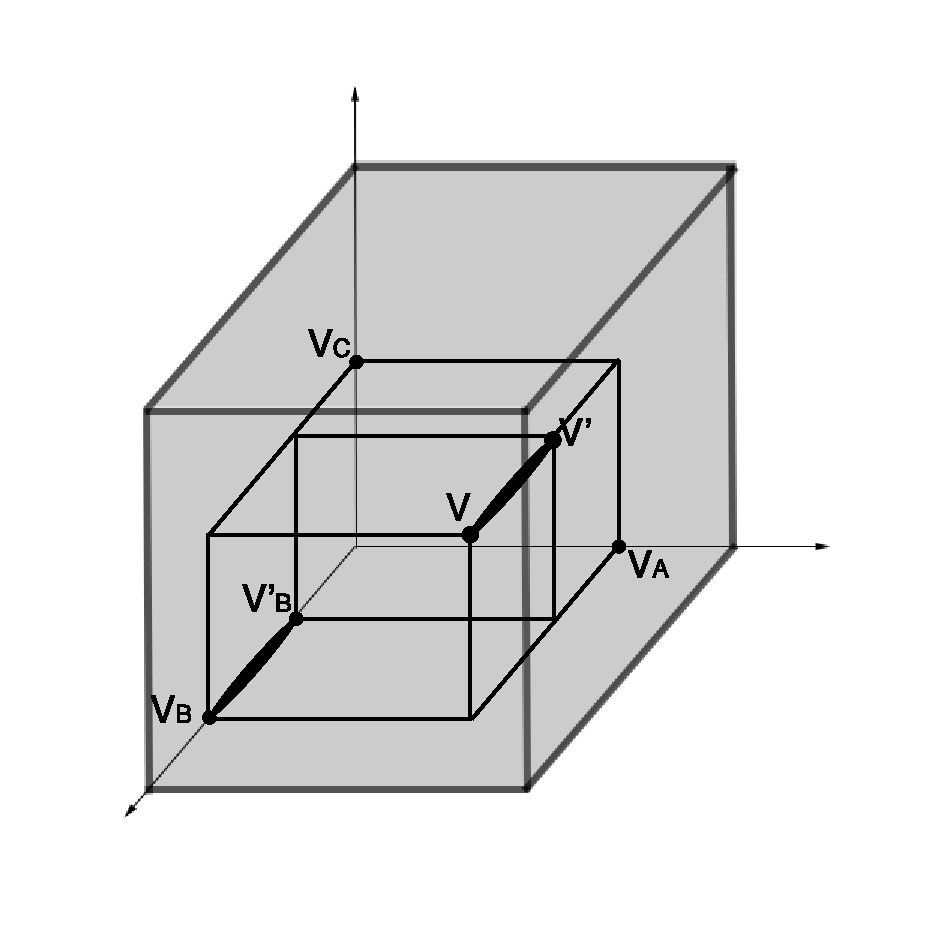
\includegraphics[scale=0.40]{Interpolation-GRID-TA.eps}
\caption{Complete grid, TA case}
\label{figNCRGRIDTA}
\end{center}
\end{figurehere}

\begin{figurehere}
\begin{center}
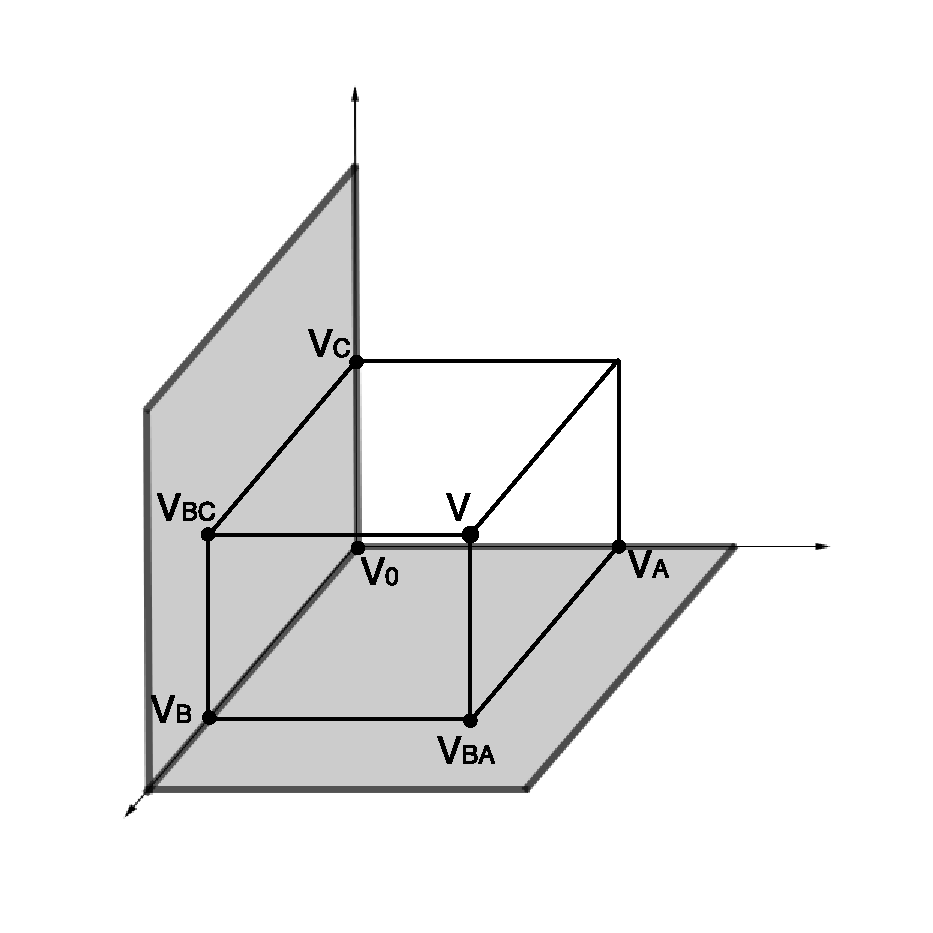
\includegraphics[scale=0.40]{Interpolation-PLANE-INS.eps}
\caption{Partial grid, complete planes, one point case}
\label{figNCRPLANEINS}
\end{center}
\end{figurehere}

\begin{figurehere}
\begin{center}
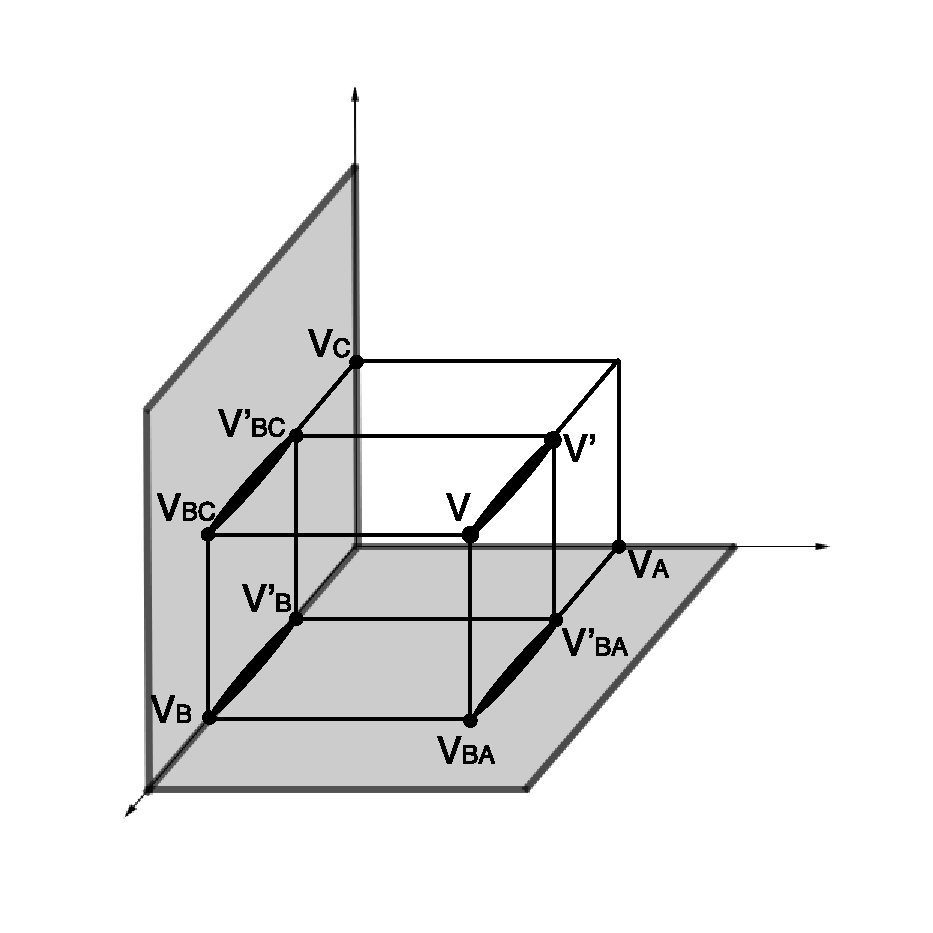
\includegraphics[scale=0.40]{Interpolation-PLANE-TA.eps}
\caption{Partial grid, complete planes, TA case}
\label{figNCRPLANETA}
\end{center}
\end{figurehere}

\begin{figurehere}
\begin{center}
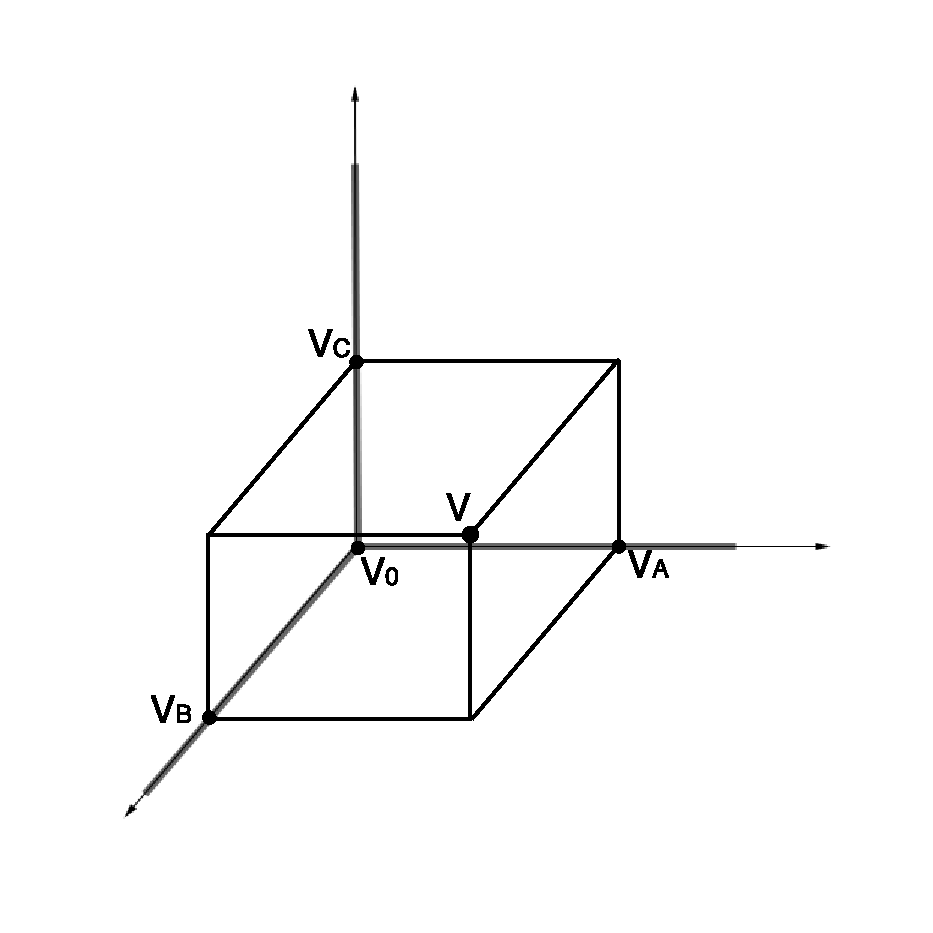
\includegraphics[scale=0.40]{Interpolation-AXE-INS.eps}
\caption{Partial grid, complete axis, one point case}
\label{figNCRAXEINS}
\end{center}
\end{figurehere}

\begin{figurehere}
\begin{center}
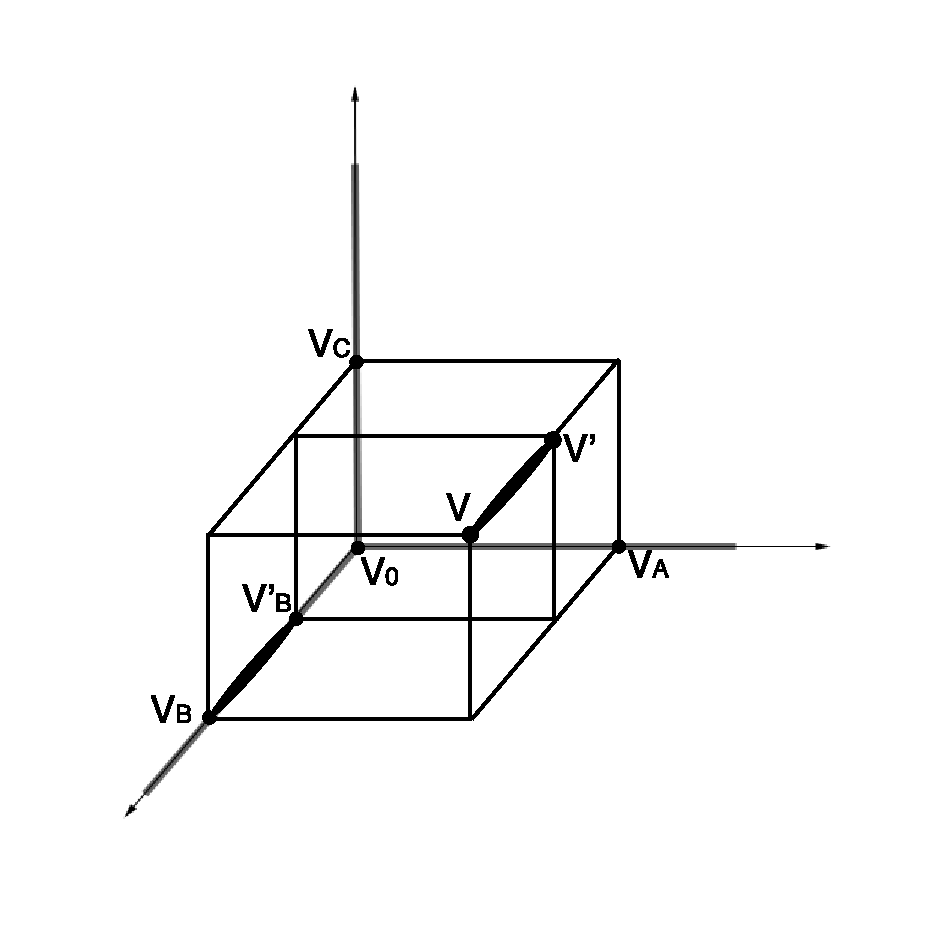
\includegraphics[scale=0.40]{Interpolation-AXE-TA.eps}
\caption{Partial grid, complete axis, TA case}
\label{figNCRAXETA}
\end{center}
\end{figurehere}

\begin{figurehere}
\begin{center}
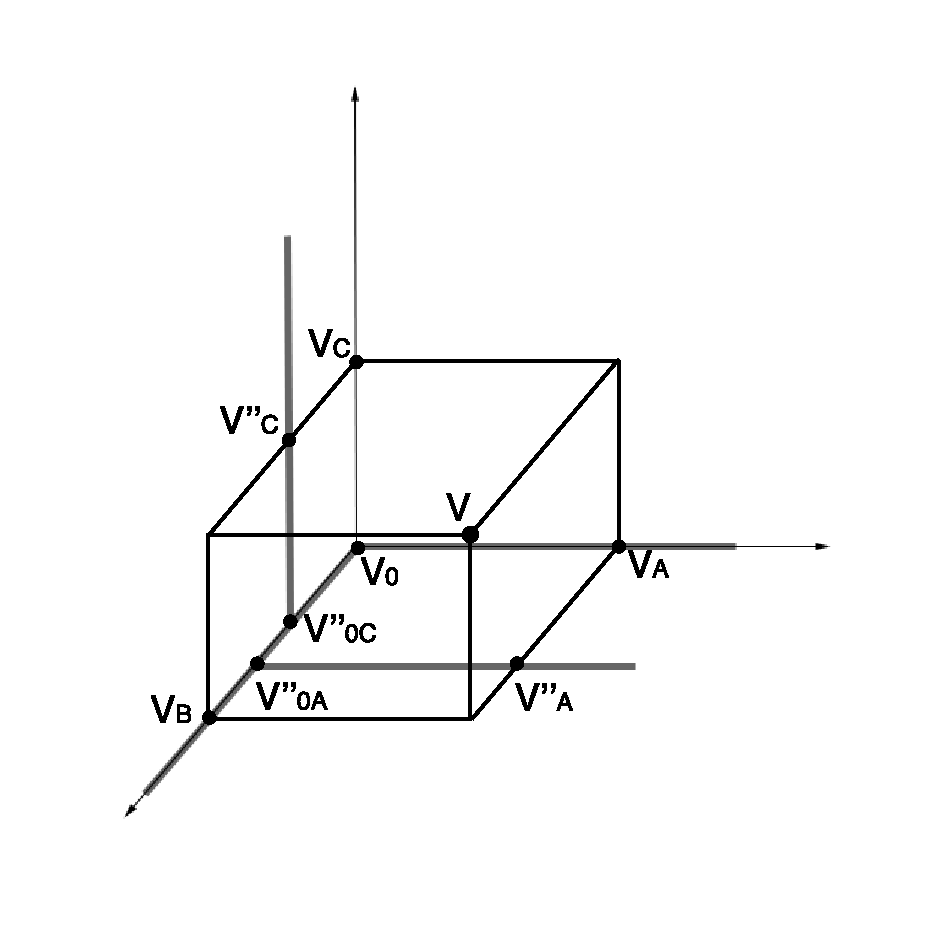
\includegraphics[scale=0.40]{Interpolation-AXE-INSbis.eps}
\caption{Partial grid, complete axis with another configuration, one point case}
\label{figNCRAXEINSbis}
\end{center}
\end{figurehere}

\begin{figurehere}
\begin{center}
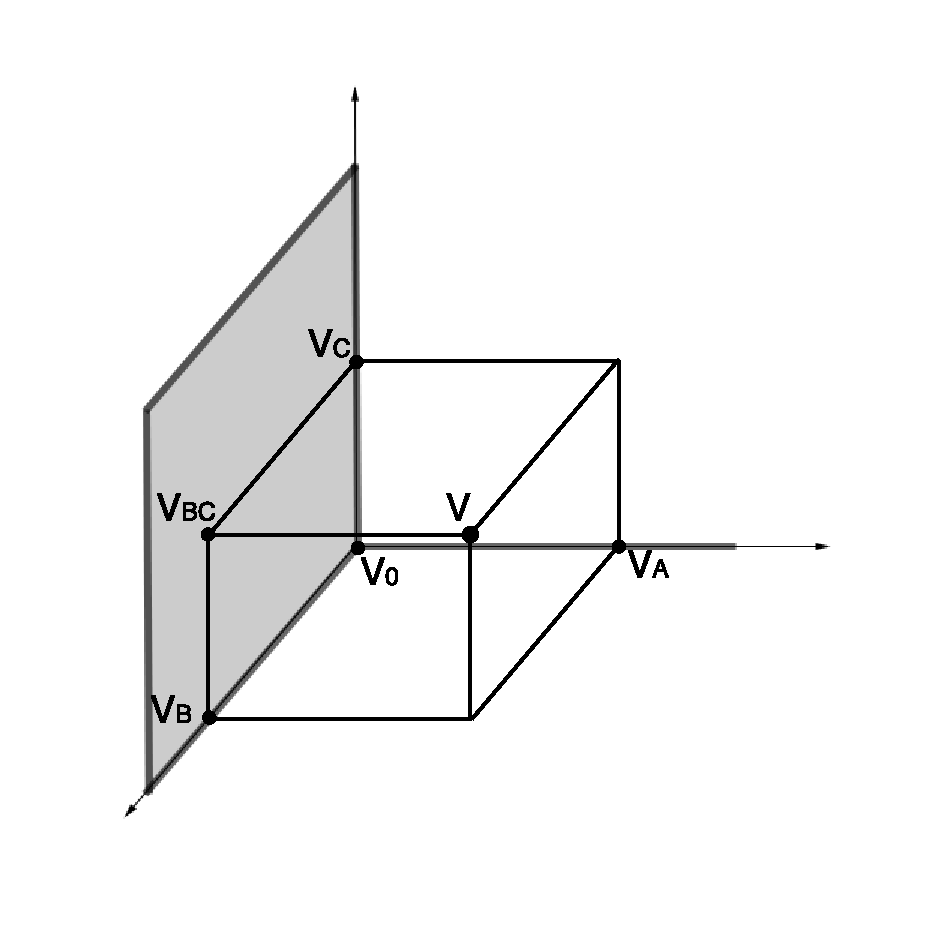
\includegraphics[scale=0.40]{Interpolation-PLAX-INS.eps}
\caption{Partial grid, one complete plane and one complete axis, one point case}
\label{figNCRPLAXINS}
\end{center}
\end{figurehere}

\begin{figurehere}
\begin{center}
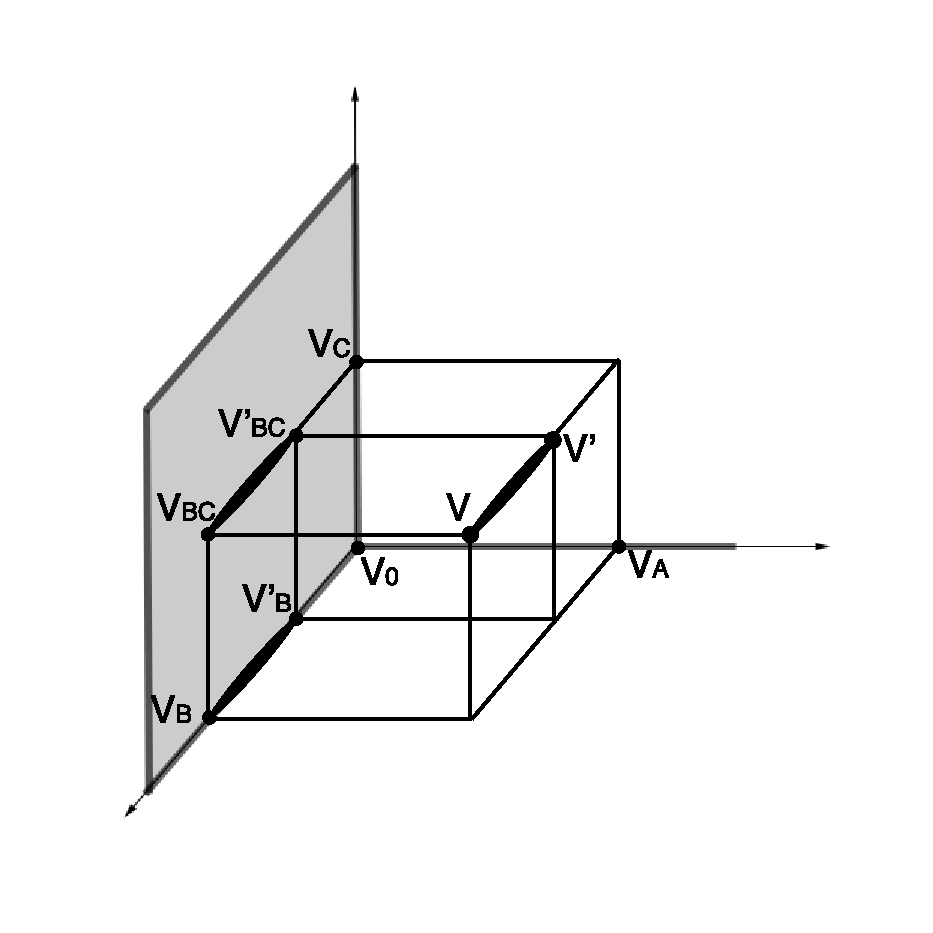
\includegraphics[scale=0.40]{Interpolation-PLAX-TA.eps}
\caption{Partial grid, one complete plane and one complete axis, TA case}
\label{figNCRPLAXTA}
\end{center}
\end{figurehere}

\begin{figurehere}
\begin{center}
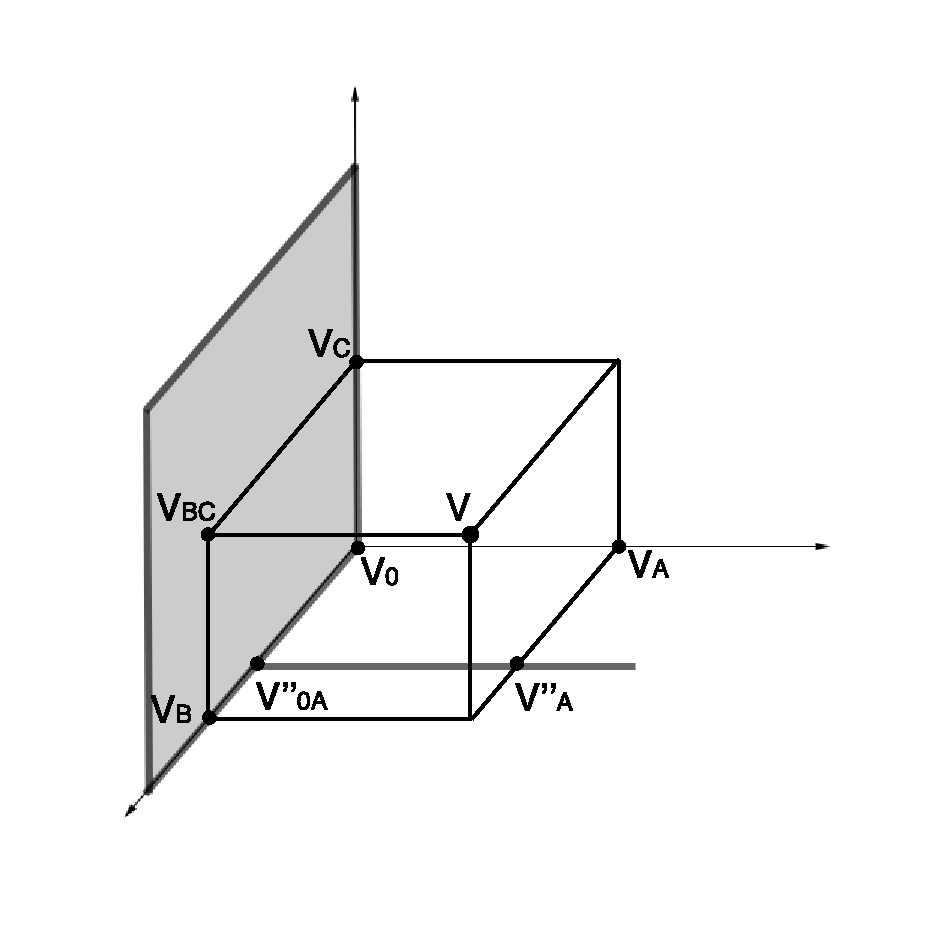
\includegraphics[scale=0.40]{Interpolation-PLAX-INSbis.eps}
\caption{Partial grid, one complete plane and one complete axis with another configuration, one point case}
\label{figNCRPLAXINSbis}
\end{center}
\end{figurehere}

}
\end{multicols}

\clearpage

\vskip 1.0cm
\subsection{The {\tt SCR:} module}\label{sect:SCRData}

This component of DONJON is dedicated to the interpolation of
{\sc macrolib} data from a {\sc saphyb} object, the reactor database produced by module {\tt SAP:}
in DRAGON or by module {\tt SAPHYB:} in APOLLO2.\cite{apollo2} A set of {\sl global parameters} are defined for each material mixture and
used as multi-dimensional interpolation variables.

\vskip 0.02cm

The calling specifications are:

\begin{DataStructure}{Structure \dstr{SCR:}}
\dusa{MLIB}~\moc{:=}~\moc{SCR:}~$[~\{$~\dusa{MLIB} $|$ \dusa{MLIB2}~$\}~]$ \dusa{SAPNAM1} $[[$~\dusa{SAPNAM2}~$]]~[$~\dusa{MAPFL}~$]$~\moc{::}~\dstr{scr\_data} \\
\end{DataStructure}

\noindent where
\begin{ListeDeDescription}{mmmmmmm}

\item[\dusa{MLIB}] {\tt character*12} name of a {\sc microlib} (type {\tt L\_LIBRARY}) or {\sc macrolib} (type {\tt L\_MACROLIB}) containing the interpolated data.
If this object also appears on the RHS of structure \dstr{SCR:}, it is open in modification mode and updated.

\item[\dusa{MLIB2}] {\tt character*12} name of an optional {\sc microlib} object whose content is copied on \dusa{MLIB}.

\item[\dusa{SAPNAM1}] {\tt character*12} name of the {\sc lcm} object containing the
{\sc saphyb} data structure ({\tt L\_SAPHYB} signature).

\item[\dusa{SAPNAM2}] {\tt character*12} name of an additional {\sc lcm} object containing an auxiliary
{\sc saphyb} data structure ({\tt L\_SAPHYB} signature). This object is optional.

\item[\dusa{MAPFL}] {\tt character*12} name of the {\sc map} object containing fuel regions description, global parameter
information (burnup, fuel/coolant temperatures, coolant density, etc). Keyword \moc{TABLE} is expected in \dstr{scr\_data}.

\item[\dusa{scr\_data}] input data structure containing interpolation information (see \Sect{descscr}).

\end{ListeDeDescription}

Note: {\sc saphyb} files generated by APOLLO2 don't have a signature. If such a {\sc saphyb} is given as input
to module {\tt SCR:}, a signature must be included before using it. The following instruction
can do the job:
\begin{verbatim}
Saphyb := UTL: Saphyb :: CREA SIGNATURE 3 = 'L_SA' 'PHYB' ' ' ;
\end{verbatim}

\subsubsection{Interpolation data input for module {\tt SCR:}}\label{sect:descscr}

\vskip -0.5cm

\begin{DataStructure}{Structure \dstr{scr\_data}}
$[$~\moc{EDIT} \dusa{iprint}~$]$ \\
$[$~\moc{RES} $]~[$~\moc{PURE}~$]~[$~\moc{UPS}~$]$ \\
$[~\{$~\moc{MACRO}~$|$~\moc{MICRO}~$\}~]~[~\{$~\moc{LINEAR}~$|$~\moc{CUBIC}~$\}~]~[$~\moc{LEAK}~\dusa{b2}~$]~[$~\moc{EQUI}~\dusa{TEXT4}~$]~[$~\moc{MASL}~\dusa{TEXT4}~$]$ \\
$[$~\moc{NMIX} \dusa{nmixt}~$]$ \\
$\{~[[$~\moc{SAPHYB} \dusa{SAPNAM} \dstr{descints}~$]]~|~[[$~\moc{TABLE} \dusa{SAPNAM} $[$ \dusa{namburn} $]$ \dstr{descints} ~$]]~\}$ \\
$[$ \dstr{descdepl} $]$ \\
{\tt ;}
\end{DataStructure}

\noindent where
\begin{ListeDeDescription}{mmmmmmmm}

\item[\moc{EDIT}] keyword used to set \dusa{iprint}.

\item[\dusa{iprint}] index used to control the printing in module {\tt SCR:}. =0 for no print; =1 for minimum printing (default value).
 
\item[\moc{RES}] keyword indicating that the interpolation is done only for the microscopic cross sections and not for the isotopic densities. In this case, a RHS {\sc microlib} must be defined and the number densities are recovered from it. This option is useful for micro-depletion applications. {\bf Important note:} It is possible to force interpolation of some isotopic densities with \moc{RES} option if these
isotopes are explicitely specified with a ``\moc{*}'' flag after \moc{MICRO} keyword in \dusa{descints} input data structure (see \Sect{descints}).

\item[\moc{PURE}] keyword indicating that the interpolation is a pure linear combination of terp factors. The fission spectra are {\sl not}
renormalized. By default, non-linear effects are produced by renormalization operations.

\item[\moc{UPS}] keyword to specify that the macrolib and/or microlib cross sections recovered from a Saphyb are
corrected so as to eliminate up-scattering. This option is useful for reactor analysis codes which cannot
take into account such cross sections.

\item[\moc{MACRO}] keyword indicating that \dusa{MLIB} is a {\sc macrolib} (default option).

\item[\moc{MICRO}] keyword indicating that \dusa{MLIB} is a {\sc microlib}. Object \dusa{MLIB} contains an embedded {\sc macrolib}, but the CPU time required to obtain it is longer.

\item[\moc{LINEAR}] keyword indicating that interpolation of the {\sc saphyb} uses linear Lagrange polynomials (default option).

\item[\moc{CUBIC}] keyword indicating that interpolation of the {\sc saphyb} uses the Ceschino method
with cubic Hermite polynomials, as presented in Ref.~\citen{Intech2011}.

\item[\moc{LEAK}] keyword used to introduce leakage in the embedded {\sc macrolib}. This option should only be used for non-regression tests.

\item[\dusa{b2}] the imposed buckling corresponding to the leakage.

\item[\moc{EQUI}] keyword used to select a SPH factor set in the Saphyb. By default, the cross sections and diffusion coefficients
are not SPH-corrected.

\item[\moc{MASL}] keyword used to recover the heavy metal density in the local parameter data of the Saphyb. 

\item[\dusa{TEXT4}] character*4 user-defined keyword of the SPH factor set or heavy metal density selected in the Saphyb. These sets are stored as local parameter information in the Saphyb.

\item[\moc{NMIX}] keyword used to define the maximum number of material mixtures. This information is required only if \dusa{MLIB} is created.

\item[\dusa{nmixt}] the maximum number of mixtures (a mixture is characterized by a distinct set of 
macroscopic cross sections) the {\sc macrolib} may contain. The default value is \dusa{nmixt} $=0$ or the value recovered from \dusa{MLIB} if it appears on the RHS
of structure \dstr{scr\_data}.

\item[\moc{SAPHYB}] keyword used to set \dusa{SAPNAM} and to define each global parameter.

\item[\moc{TABLE}] keyword used to set \dusa{SAPNAM} and to recover some global parameter from a {\sc map} object named \dusa{MAPFL}.

\item[\dusa{SAPNAM}] {\tt character*12} name of the {\sc lcm} object containing the
{\sc saphyb} data structure where the interpolation is performed. This name must be set in the RHS of structure \dstr{SCR:}.

\item[\dusa{namburn}] name of the parameter for burnup (or irradiation).
This value is defined if option \moc{TABLE} is set {\sl and} if burnup (or irradiation) is to be considered as parameter.

\item[\dusa{descints}] input data structure containing interpolation information relative to the {\sc saphyb} data structure named \dusa{SAPNAM} (see \Sect{descints}).

\item[\dstr{descdepl}] input structure describing the depletion chain (see \Sect{descdepld}). This input structure requires option \moc{MICRO}. By
default, the depletion chain data is not written in the output {\sc microlib}.

\end{ListeDeDescription}

\subsubsection{Defining global parameters}\label{sect:descints}

\vskip -0.5cm

If a {\sc map} object is defined on the RHS of structure \dstr{SCR:}, and if the \moc{TABLE} keyword is set, some information required to set the interpolation points is found in this object.
In this case, the {\tt SCR:} operator search the {\sc saphyb} object for global parameters  having an arbitrary name specified in the {\sc map} object or set directly in this module.
Note that any parameter's value set directly in this module prevails on a value stored in the \dusa{MAPFL} object.

Each instance of \dusa{descints} is a data structure specified as

\begin{DataStructure}{Structure \dstr{descints}}
$[[$~\moc{MIX} \dusa{imix}~$[~\{$~\moc{FROM}~\dusa{imixold}~$|$~\moc{USE}~$\}~]$ \\
~~~~~~$[~\{$~\moc{TIMAV-BURN} $|$ \moc{INST-BURN} $|$ \moc{AVG-EX-BURN}~\dusa{ivarty}~$\}~]$ \\
~~~~~~$[[~\{$~\moc{SET} $|$ \moc{DELTA} $|$ \moc{ADD}~$\}~\}~[~\{$ \moc{LINEAR} $|$ \moc{CUBIC}~$\}~]$ \dusa{PARKEY} $\{$~\dusa{val1} $|$ \moc{MAP}~$\}~[~\{$~\dusa{val2} $|$ \moc{MAP}~$\}~]$ \\
~~~~~~~~~~~~$[$~\moc{REF} $[[$~\dusa{PARKEY}~$\{$~\dusa{valref} $|$ \moc{SAMEASREF}~$\}$~$]]$~\moc{ENDREF}~$]~]]$  \\
~~~~~~$[$~\moc{MICRO}~$\{$~\moc{ALL} $|$ \moc{ONLY}~$\}~[[$~\dusa{HISO} $\{$ \dusa{conc} $|$ \moc{*} $\}~[$ \moc{NOEV} $]~]]~]$ \\
\moc{ENDMIX}~$]]$
\end{DataStructure}

\noindent where
\begin{ListeDeDescription}{mmmmmmmm}

\item[\moc{MIX}] keyword used to set \dusa{imix}. Discontinuity factor information present in the Saphyb is interpolated as mixture~1 values.

\item[\dusa{imix}] index of the mixture that is to be created in the {\sc microlib} and {\sc macrolib}.

\item[\moc{FROM}] keyword used to set the index of the mixture in the {\sc saphyb} object.

\item[\dusa{imixold}] index of the mixture that is recovered in the {\sc saphyb} object. By default, \dusa{imixold}$=1$.

\item[\moc{USE}] keyword used to set the index of the mixture in the {\sc saphyb} object equal to \dusa{imix}.

\item[\moc{TIMAV-BURN}] keyword used to compute time-averaged cross-section information. This option is available {\sl only if} a \dusa{MAPFL} object is set.
By default, the type of calculation (\moc{TIMAV-BURN} or \moc{INST-BURN}) is recovered from the \dusa{MAPFL} object.

\item[\moc{INST-BURN}] keyword used to compute cross-section information at specific bundle burnups. This option is available {\sl only if} a \dusa{MAPFL} object is set.
By default, the type of calculation (\moc{TIMAV-BURN} or \moc{INST-BURN}) is recovered from the \dusa{MAPFL} object.

\item[\moc{AVG-EX-BURN}] keyword used to compute the derivatives of cross-section information relative to the exit burnup of a single combustion zone. The derivatives are computed using Eq.~(3.3) of Ref.~\citen{chambon}, written as
$$
{\partial \bar\Sigma_x\over \partial B_j^{\rm e}}={1\over B_j^{\rm e}\, (B_{j,k}^{\rm eoc}-B_{j,k}^{\rm boc})}
\left[- \int_{B_{j,k}^{\rm boc}}^{B_{j,k}^{\rm eoc}}dB \, \Sigma_x(B)+B_{j,k}^{\rm eoc}\, \Sigma_x(B_{j,k}^{\rm eoc})-B_{j,k}^{\rm boc}\, \Sigma_x(B_{j,k}^{\rm boc})\right]
$$

\noindent where $B_{j,k}^{\rm boc}$, $B_{j,k}^{\rm eoc}$, and $B_j^{\rm e}$ are the beginning of cycle burnup of bundle $\{j,k\}$, end of cycle burnup of bundle $\{j,k\}$ and exit burnup of channel $j$. This option is available {\sl only if} a \dusa{MAPFL} object is set.
By default, the type of calculation (\moc{TIMAV-BURN} or \moc{INST-BURN}) is recovered from the \dusa{MAPFL} object.

\item[\dusa{ivarty}] index of the combustion zone for differentiation of cross-section information.

\item[\moc{SET}] keyword used to indicate a simple interpolation at \dusa{val1} or an averaging between \dusa{val1} and \dusa{val2}. The result $\sigma_{\rm ref}$ is also used as the reference value when the \moc{ADD} is used. Note: see at the ending note of this section for a detailed description and examples.

\item[\moc{DELTA}] keyword used to indicate a delta-sigma calculation between \dusa{val2} and \dusa{val1}
(i.e., $\Delta\sigma_{\rm ref}=\sigma_{\rm val2}-\sigma_{\rm val1}$ is computed). This keyword can be used only once in each mixture data block (initiated
with a \moc{MIX} keyword). Note: see at the ending note of this section for a detailed description and examples.

\item[\moc{ADD}] keyword used to indicate a delta-sigma calculation between \dusa{val2} and \dusa{val1} is added to the reference value
(i.e., $\Delta\sigma=\sigma_{\rm val2}-\sigma_{\rm val1}$ is used as contribution, $\sigma_{\rm ref}+\Delta\sigma$ or $\Delta\sigma_{\rm ref}+\Delta\sigma$ is returned). Note: see at the ending note of this section for a detailed description and examples.

\item[\moc{LINEAR}] keyword indicating that interpolation of the {\sc saphyb} for parameter \dusa{PARKEY} uses linear Lagrange
polynomials. It is possible to set different interpolation modes to different parameters. By default, the interpolation mode is set in Sect.~\ref{sect:descscr}.

\item[\moc{CUBIC}] keyword indicating that interpolation of the {\sc saphyb} for parameter \dusa{PARKEY} uses the Ceschino method
with cubic Hermite polynomials, as presented in Ref.~\citen{Intech2011}. By default, the interpolation mode is set in Sect.~\ref{sect:descscr}.

\item[\dusa{PARKEY}] {\tt character*12} user-defined keyword associated to a global
parameter to be set.

\item[\dusa{val1}] value of a global parameter used to interpolate.  \dusa{val1} is the initial value of this parameter in case an average is required. \dusa{val1} can be an integer, real or string value.

\item[\dusa{val2}] value of the final global parameter. By default, a simple interpolation is performed, so that \dusa{val2}$=$\dusa{val1}. \dusa{val2} is always a real value with \dusa{val2}$\ge$\dusa{val1}.

\item[\moc{MAP}] keyword used to indicate that the value of parameter \dusa{val1} or the second value for the $\Delta\sigma$ calculation is
recovered from \dusa{MAPFL}, i.e. the {\sc map} object containing fuel regions description.

\item[\moc{REF}] keyword only available together with the \moc{ADD} option. It is used to set all the other variable values when a $\Delta$ contribution is performed for one variable.  

\item[\dusa{valref}] value of the reference parameter, when it is directly given by the user. Note that there is no default value.

\item[\moc{SAMEASREF}] keyword used to specify that the reference value will be the same as in the refence case, i.e. for the $\sigma_{\rm ref}$ computation.

\item[\moc{ENDREF}] keyword only available together with the \moc{ADD} option. It is used to specify that all the other variable values which are required are given.  

\item[\moc{MICRO}] keyword used to set the number densities of some isotopes present in the {\sc saphyb} object. The data statement ``\moc{MICRO} \moc{ALL}" is used by default.

\item[\moc{ALL}] keyword to indicate that all the isotopes present in the  {\sc saphyb} object will be used in the {\sc microlib} and {\sc macrolib} objects. Concentrations of these isotopes will be recovered from the {\sc saphyb} object or set using
the ``\dusa{HISO} \dusa{conc}" data statement.

\item[\moc{ONLY}] keyword to indicate that only the isotopes set using the ``\dusa{HISO} \dusa{conc}" data statement will be used in the {\sc microlib} and {\sc macrolib} objects.

\item[\dusa{HISO}] {\tt character*8} name of an isotope.

\item[\dusa{conc}] user-defined value of the number density (in $10^{24}$ particles per ${\rm cm}^3$) of the isotope.

\item[\moc{*}] the value of the number density for isotope \dusa{HISO} is recovered from the {\sc saphyb} object.

\item[\moc{NOEV}] keyword to force the isotope \dusa{HISO} to be non-depleting.

\item[\moc{ENDMIX}] end of specification keyword for the material mixture.

\end{ListeDeDescription}

\subsubsection{Depletion data structure}\label{sect:descdepld}

Part of the depletion data used in the isotopic depletion calculation (the fission yields and the
radioactive decay constants) is recovered from the Saphyb file. Remaining depletion data is
recovered from the input data structure \dstr{descdepl}. This data describes the heredity of the radioactive decay
and the neutron activation chain.

\begin{DataStructure}{Structure \dstr{descdepl}}
\moc{CHAIN} \\
\hskip 0.3cm $[[$ \dusa{NAMDPL} $[$ \dusa{izae} $]$ \\
\hskip 0.6cm $[[$ \dusa{reaction} $[$ \dusa{energy} $]~]]$ \\
\hskip 0.6cm $[~\{$ \moc{STABLE} $|$ \moc{FROM} $[[~\{$ \moc{DECAY} $|$ \dusa{reaction} $\}$
$[[$ \dusa{yield} \dusa{NAMPAR} $]]~]]~\}~]~]]$\\
\moc{ENDCHAIN}
\end{DataStructure}

\noindent
with:

\begin{ListeDeDescription}{mmmmmm}

\item[\moc{CHAIN}] keyword to specify the beginning of the depletion chain.

\item[\dusa{NAMDPL}] {\tt character*12} name of an isotope (or isomer) of the
depletion chain that appears as a particularized isotope of the Saphyb.

\item[\dusa{izae}] optional six digit integer representing the isotope. The first two
digits represent the atomic number of the isotope; the next three indicate its
mass number and the last digit indicates the  excitation level of the nucleus (0
for a nucleus in its ground state, 1 for an isomer in its first exited state,
etc.). For example, $^{238}$U in its ground state will be represented by
\dusa{izae}=922380.

\item[\dusa{reaction}] {\tt character*6} identification of a neutron-induced
reaction that takes place either for production of this isotope, its depletion,
or for producing energy. Example of reactions are following:

\begin{ListeDeDescription}{mmmmmmmm}
\item[\moc{NG}] indicates that a radiative capture reaction takes place either
for production of this isotope, its depletion or for producing energy.

\item[\moc{N2N}] indicates that the following reaction is taking place:
$$ n +^{A}X_Z \to 2 n + ^{A-1}X_Z$$

\item[\moc{N3N}] indicates that the following reaction is taking place:
$$ n +^{A}X_Z \to 3 n + ^{A-2}X_Z$$

\item[\moc{N4N}] indicates that the following reaction is taking place:
$$ n +^{A}X_Z \to 4 n + ^{A-3}X_Z$$

\item[\moc{NP}] indicates that the following reaction is taking place:
$$ n +^{A}X_Z \to p + ^AY_{Z-1}$$

\item[\moc{NA}] indicates that the following reaction is taking place:
$$ n +^{A}X_Z \to ^4{\rm He}_2 + ^{A-3}X_{Z-2}$$

\item[\moc{NFTOT}] indicates that a fission is taking place.
\end{ListeDeDescription}

\item[\dusa{energy}] energy (in MeV) recoverable per neutron-induced
reaction of type \dusa{reaction}. If the energy associated to radiative capture
is not explicitely given, it should be added to the energy released per fission. By
default, \dusa{energy}=0.0 MeV.

\item[\moc{STABLE}] non depleting isotope. Such an isotope may produces
energy by neutron-induced reactions (such as radiative capture).

\item[\moc{FROM}] indicates that this isotope is produced from decay or
neutron-induced reactions.

\item[\moc{DECAY}] indicates that a decay reaction takes place for its
production.

\item[\dusa{yield}] branching ratio or production yield expressed in fraction.

\item[\dusa{NAMPAR}] {\tt character*12} name of the a parent isotope
(or isomer) that appears as a particularized isotope of the Saphyb.

\item[\moc{ENDCHAIN}] keyword to specify the end of the depletion chain.

\end{ListeDeDescription}


\subsubsection{Interpolation in the parameter grid}

The following example corresponds to a delta-sigma computation in mixture 1 corresponding to a perturbation. Note that in this case, the \moc{MACROLIB} object  may content negative cross-section. 
\begin{verbatim}
MACROLIB := SCR: SAP ::
   EDIT 40 NMIX 1 SAPHYB SAP
   MIX 1  !(* delta sigma contribution *)
          SET 'CELL' '3D'
          DELTA 'PITCH' 0.0 1.0
   ENDMIX
;
\end{verbatim}

When the number of parameters used for the interpolation is increased, all the lattice computations corresponding to all the combinations of parameters may not be done for computation time reasons. In this case, some approximations may be required. The choice for the \moc{SET}, \moc{DELTA} and \moc{ADD} is then dependent of the structure of the database (i.e. how the database grid of possibilities is filled). When a {\sc map} object containing fuel regions description is used, the problem become even more complex, because values have to be automatically changed for all bundles. In order to clarify all the different possibilities and limitations dependently of the database structure, we will use a 3 parameter case. The paramaters are referenced by 'A', 'B' and 'C'. But before we explain the different cases, we want to remind that the interpolation factors are computed on each axis seperatly.

The first case corresponds to a complete grid, represented by a gray paralepiped on Fig. \ref{figNCRGRIDINS} and \ref{figNCRGRIDTA}. The
figure \ref{figNCRGRIDINS} shows that the interpolated value in point $V$ can be obtained directly without {\sc map} object. For time-average (TA) computation, lets assume that the parameter 'B' represents the burnup (and keep this convention for other database structure also). In this case the figure \ref{figNCRGRIDTA} shows also that the direct interpolation can be done to compute an average value between the points $V'$ and $V$. Note that the TA burnups are stored in the {\sc map} object, and are then recovered automatically.

The second case corresponds to a partial grid where all the lattice computations have been perfomed for several pairs of parameters, which are represented as the gray rectangles on Fig. \ref{figNCRPLANEINS} and \ref{figNCRPLANETA}. If we use the notations of Fig. \ref{figNCRPLANEINS} and \ref{figNCRPLANETA}, the best estimate interpolated values, $f$, we can get are given by: \\
$f=f(V)~\approx~f(V_B)+(f(V_{BA})-f(V_B))+(f(V_{BC})-f(V_B))=f(V_{BC})+(f(V_{BA})-f(V_B))=f(V_{BA})+(f(V_{BC})-f(V_B))$ for instataneous\\
$f=f(V',V)~\approx~f(V'_B,V_B)+(f(V'_{BA},V_{BA})-f(V'_B,V_B))+(f(V'_{BC},V_{BC})-f(V'_B,V_B))=f(V'_{BC},V_{BC})+(f(V'_{BA},V_{BA})-f(V'_B,V_B))=f(V'_{BA},V_{BA})+(f(V'_{BC},V_{BC})-f(V'_B,V_B))$ for TA\\
~~~~where $f(.,.)$ represents the average value between two points.

The third case corresponds to a minimal grid, where the lattice computations have been perfomed only for one parameter variation at a time. In this case, the grid is represented by the thick gray lines on the axis on Fig. \ref{figNCRAXEINS} and \ref{figNCRAXETA}. If we use the notations of Fig. \ref{figNCRAXEINS} and \ref{figNCRAXETA}, the best estimate interpolated values, $f$, we can get are given by: \\
$f=f(V)~\approx~f(V_0)+(f(V_A)-f(V_0))+(f(V_B)-f(V_0))+(f(V_C)-f(V_0))=f(V_B)+(f(V_A)-f(V_0))+(f(V_C)-f(V_0))$ for instataneous\\
$f=f(V',V)~\approx~f(V'_B,V_B)+(f(V_A)-f(V_0))+(f(V_C)-f(V_0))$ for TA\\
Note that the reference point ($V_0$ in the example) does not have to be the same for all parameters. Database structures such as represented on Fig \ref{figNCRAXEINSbis} can also been used. In this case, we even have two choices for the $\Delta f$ computation on axis 'A'. 

The last case is in fact a mix of cases 2 and 3. The gray rectangle and the gray line on Fig. \ref{figNCRPLAXINS} and \ref{figNCRPLAXTA} reprensent where all the lattice computations have been performed. With the notations used on those figures, one can write that the best estimate interpolated values, $f$, we can get are given by: \\
$f=f(V)~\approx~f(V_B)+(f(V_{BC})-f(V_B))+(f(V_A)-f(V_0))=f(V_{BC})+(f(V_A)-f(V_0))$ for instataneous\\
$f=f(V',V)~\approx~f(V'_B,V_B)+(f(V'_{BC},V_{BC})-f(V'_B,V_B))+(f(V_A)-f(V_0))=f(V'_{BC},V_{BC})+(f(V_A)-f(V_0))$ for TA\\
Note once again that the reference point ($V_0$ in the example) does not have to be the same for all parameters. Database structures such as represented on Fig \ref{figNCRPLAXINSbis} can also been used.
\clearpage

The input files will actually reflect the previous equations. However, they are different if the parameters are stored in a {\sc map} object, \dusa{MAPFL}, or provided directly by the user. For the case of one point interpolation (i.e. instantaneous), the input files will be: \\

\begin{center}
\tablefirsthead{%
\hline
case & all parameters explicitly set & all parameters in {\sc map}\\
\hline}
\tablehead{%
%\hline
%\multicolumn{3}{|l|}{\small\sl continued from previous page}\\
\hline
case & all parameters explicitly set & all parameters in {\sc map}\\
\hline}
\tabletail{%
\hline
\multicolumn{3}{|r|}{\small\sl continued on next page}\\
\hline}
\tablelasttail{\hline}
\bottomcaption{SCR inputs for instantaneous cases}

\begin{supertabular}{|p{0.1\textwidth}|p{0.4\textwidth}|p{0.4\textwidth}|}
%\begin{tabular}{|p{0.1\textwidth}|p{0.4\textwidth}|p{0.4\textwidth}|}
%\hline
%case & all parameters explicitly set & all parameters in {\sc map}\\
\hline
GRID (Fig. \ref{figNCRGRIDINS}) 
& \begin{verbatim}
MACROLIB := SCR: SAP ::
   NMIX 1 
   SAPHYB SAP
   MIX 1 
      SET 'A' <<va>>
      SET 'B' <<vb>>
      SET 'C' <<vc>>
   ENDMIX
;
\end{verbatim} 
& \begin{verbatim}
MACROLIB := SCR: SAP FMAP ::
   NMIX 1
   TABLE SAP 'B' 
   MIX 1 
   ENDMIX
;
\end{verbatim} \\
\hline
PLANE (Fig. \ref{figNCRPLANEINS}) & 
\begin{verbatim}
MACROLIB := SCR: SAP ::
   NMIX 1
   SAPHYB SAP
   MIX 1 
      SET 'A' <<va>>
      SET 'B' <<vb>>
      SET 'C' <<vc0>>
      ADD 'C' <<vc0>> <<vc>>
         REF  'A' <<va0>> 
              'B' <<vb>> ENDREF
!or           'B' SAMEASREF ENDREF
   ENDMIX
;
\end{verbatim} &
\begin{verbatim}
MACROLIB := SCR: SAP FMAP ::
   NMIX 1
   TABLE SAP 'B' 
   MIX 1 
      SET 'C' <<vc0>>
      ADD 'C' <<vc0>> MAP
         REF  'A' <<va0>> 
              'B' SAMEASREF ENDREF
!or   SET 'A' <<va0>>
!or   ADD 'A' <<va0>> MAP
!or      REF  'C' <<vc0>> 
!or           'B' SAMEASREF ENDREF
   ENDMIX
;
\end{verbatim} \\
\hline
%\end{tabular}
%
%\begin{tabular}{|p{0.1\textwidth}|p{0.4\textwidth}|p{0.4\textwidth}|}
%\hline
%case & all parameters explicitly set & all parameters in {\sc map}\\
%\hline
AXE (Fig. \ref{figNCRAXEINS}) & 
\begin{verbatim}
MACROLIB := SCR: SAP ::
   NMIX 1 
   SAPHYB SAP
   MIX 1 
      SET 'A' <<va0>>
      SET 'B' <<vb>>
      SET 'C' <<vc0>>
      ADD 'A' <<va0>> <<va>>
         REF  'C' <<vc0>> 
              'B' <<vb0>> ENDREF
      ADD 'C' <<vc0>> <<vc>>
         REF  'A' <<va0>> 
              'B' <<vb0>> ENDREF
   ENDMIX
;
\end{verbatim} &
\begin{verbatim}
MACROLIB := SCR: SAP FMAP ::
   NMIX 1
   TABLE SAP 'B' 
   MIX 1 
      SET 'A' <<va0>>
      SET 'C' <<vc0>>
      ADD 'A' <<va0>> MAP
         REF  'C' <<vc0>> 
              'B' <<vb0>> ENDREF
      ADD 'C' <<vc0>> MAP
         REF  'A' <<va0>> 
              'B' <<vb0>> ENDREF
   ENDMIX
;
\end{verbatim} \\
\hline
PLANE + AXE (Fig. \ref{figNCRPLAXINS}) & 
\begin{verbatim}
MACROLIB := SCR: SAP ::
   NMIX  
   SAPHYB SAP
   MIX 1 
      SET 'A' <<va0>>
      SET 'B' <<vb>>
      SET 'C' <<vc>>
      ADD 'A' <<va0>> <<va>>
         REF  'C' <<vc0>> 
              'B' <<vb0>> ENDREF
   ENDMIX
;
\end{verbatim} &
\begin{verbatim}
MACROLIB := SCR: SAP FMAP ::
   NMIX 1
   TABLE SAP 'B' 
   MIX 1 
      SET 'A' <<va0>>
      ADD 'A' <<va0>> MAP
         REF  'C' <<vc0>> 
              'B' <<vb0>> ENDREF
   ENDMIX
;
\end{verbatim} \\
\hline
%\end{tabular}
\end{supertabular}
\end{center}

For the TA, the burnup variable has no other choice than to be stored in the {\sc map} object, \dusa{MAPFL}. Then the input files will be: \\

\begin{center}
\tablefirsthead{%
\hline
case & only the burnup in {\sc map} & all parameters in {\sc map}\\
\hline}
\tablehead{%
%\hline
%\multicolumn{3}{|l|}{\small\sl continued from previous page}\\
\hline
case & only the burnup in {\sc map} & all param. in {\sc map}\\
\hline}
\tabletail{%
\hline
\multicolumn{3}{|r|}{\small\sl continued on next page}\\
\hline}
\tablelasttail{\hline}
\bottomcaption{SCR inputs for TA cases}

\begin{supertabular}{|p{0.1\textwidth}|p{0.4\textwidth}|p{0.4\textwidth}|}
%\begin{tabular}{p{0.1\textwidth}|p{0.4\textwidth}|p{0.4\textwidth}}
%\hline
%case & only the burnup in {\sc map} & all parameters in {\sc map}\\
\hline
GRID (Fig. \ref{figNCRGRIDTA}) & 
\begin{verbatim}
MACROLIB := SCR: SAP FMAP ::
   NMIX 1
   TABLE SAP 'B' 
   MIX 1 
      SET 'A' <<va>>
      SET 'C' <<vc>>
   ENDMIX
;
\end{verbatim} &
\begin{verbatim}
MACROLIB := SCR: SAP FMAP ::
   NMIX 1
   TABLE SAP 'B' 
   MIX 1 
   ENDMIX
;
\end{verbatim} \\
\hline
PLANE (Fig. \ref{figNCRPLANETA}) & 
\begin{verbatim}
MACROLIB := SCR: SAP FMAP ::
   NMIX 1
   TABLE SAP 'B' 
   MIX 1 
      SET 'A' <<va>>
      SET 'C' <<vc0>>
      ADD 'C' <<vc0>> <<vc>>
         REF  'A' <<va0>> 
              'B' SAMEASREF ENDREF
   ENDMIX
;
\end{verbatim} &
\begin{verbatim}
MACROLIB := SCR: SAP FMAP ::
   NMIX 1
   TABLE SAP 'B' 
   MIX 1 
      SET 'C' <<vc0>>
      ADD 'C' <<vc0>> MAP
         REF  'A' <<va0>> 
              'B' SAMEASREF ENDREF
!or   SET 'A' <<va0>>
!or   ADD 'A' <<va0>> MAP
!or      REF  'C' <<vc0>> 
!or           'B' SAMEASREF ENDREF
   ENDMIX
;
\end{verbatim} \\
\hline
AXE (Fig. \ref{figNCRAXETA}) & 
\begin{verbatim}
MACROLIB := SCR: SAP FMAP ::
   NMIX 1
   TABLE SAP 'B' 
   MIX 1 
      SET 'A' <<va0>>
      SET 'C' <<vc0>>
      ADD 'A' <<va0>> <<va>>
         REF  'C' <<vc0>> 
              'B' <<vb0>> ENDREF
      ADD 'C' <<vc0>> <<vc>>
         REF  'A' <<va0>> 
              'B' <<vb0>> ENDREF
   ENDMIX
;
\end{verbatim} &
\begin{verbatim}
MACROLIB := SCR: SAP FMAP ::
   NMIX 1 
   TABLE SAP 'B' 
   MIX 1 
      SET 'A' <<va0>>
      SET 'C' <<vc0>>
      ADD 'A' <<va0>> MAP
         REF  'C' <<vc0>> 
              'B' <<vb0>> ENDREF
      ADD 'C' <<vc0>> MAP
         REF  'A' <<va0>> 
              'B' <<vb0>> ENDREF
   ENDMIX
;
\end{verbatim} \\
\hline
PLANE + AXE (Fig. \ref{figNCRPLAXTA}) & 
\begin{verbatim}
MACROLIB := SCR: SAP FMAP ::
   NMIX 1
   TABLE SAP 'B' 
   MIX 1 
      SET 'A' <<va0>>
      SET 'C' <<vc>>
      ADD 'A' <<va0>> <<va>>
         REF  'C' <<vc0>> 
              'B' <<vb0>> ENDREF
   ENDMIX
;
\end{verbatim} &
\begin{verbatim}
MACROLIB := SCR: SAP FMAP ::
   NMIX 1
   TABLE SAP 'B' 
   MIX 1 
      SET 'A' <<va0>>
      ADD 'A' <<va0>> MAP
         REF  'C' <<vc0>> 
              'B' <<vb0>> ENDREF
   ENDMIX
;
\end{verbatim} \\
\hline
%\end{tabular}
\end{supertabular}
\end{center}

\clearpage

\vskip 1.0cm
\subsection{The {\tt ACR:} module}\label{sect:ACRData}

The APOLLO2 Portable data EXchange file (APEX) contains the results obtained by a set of APOLLO2 calculation steps as well as restart data.

The APEX file is written in {\sc hdf5} format, allowing full portability and hierarchical data organization. It can be edited and modified using
the HDFView tool.

This file constitutes a natural boundary between the spectral code and the downstream codes. Particularly, it contains all the data needed by the
code in charge of cross-sections (XS) library generation for 3D core simulators.
Each elementary calculation is characterized by a set of parameters. Parameterization allows external codes building their own XS representation
by defining XS dependencies through appropriate functions or laws. For instance, standard parameters for PWR reactors are burn-up, water temperature,
water density, boron concentration, xenon concentration, fuel temperature and history parameters. BWR specific parameters are instant void fraction and
void history.

This component of DONJON is dedicated to the interpolation of {\sc macrolib} data from an APEX file, the reactor database produced by APOLLO2-A.\cite{apollo2A}
A set of {\sl global parameters} are defined for each material mixture and used as multi-dimensional interpolation variables.

\vskip 0.02cm

The calling specifications are:

\begin{DataStructure}{Structure \dstr{ACR:}}
\dusa{MLIB}~\moc{:=}~\moc{ACR:}~$[~\{$~\dusa{MLIB} $|$ \dusa{MLIB2}~$\}~]$ \dusa{APXNAM1} $[[$~\dusa{APXNAM2}~$]]~[$~\dusa{MAPFL}~$]$~\moc{::}~\dstr{acr\_data} \\
\end{DataStructure}

\noindent where
\begin{ListeDeDescription}{mmmmmmm}

\item[\dusa{MLIB}] {\tt character*12} name of a {\sc microlib} (type {\tt L\_LIBRARY}) or {\sc macrolib} (type {\tt L\_MACROLIB}) containing the interpolated data.
If this object also appears on the RHS of structure \dstr{ACR:}, it is open in modification mode and updated.

\item[\dusa{MLIB2}] {\tt character*12} name of an optional {\sc microlib} object whose content is copied on \dusa{MLIB}.

\item[\dusa{APXNAM1}] {\tt character*12} name of the {\sc hdf5} file containing the {\sc apex} data structure.

\item[\dusa{APXNAM2}] {\tt character*12} name of an additional {\sc hdf5} file containing an auxiliary
{\sc apex} data structure. This object is optional.

\item[\dusa{MAPFL}] {\tt character*12} name of the {\sc map} object containing fuel regions description, global parameter
information (burnup, fuel/coolant temperatures, coolant density, etc). Keyword \moc{TABLE} is expected in \dstr{acr\_data}.

\item[\dusa{acr\_data}] input data structure containing interpolation information (see \Sect{descacr}).

\end{ListeDeDescription}

\subsubsection{Interpolation data input for module {\tt ACR:}}\label{sect:descacr}

\vskip -0.5cm

\begin{DataStructure}{Structure \dstr{acr\_data}}
$[$~\moc{EDIT} \dusa{iprint}~$]$ \\
$[$~\moc{RES} $]~[$~\moc{PURE}~$]~[$~\moc{UPS}~$]$ \\
$[~\{$~\moc{MACRO}~$|$~\moc{MICRO}~$[$ \moc{TOTAL} $]~\}~]~[~\{$~\moc{LINEAR}~$|$~\moc{CUBIC}~$\}~]~[$~\moc{LEAK}~\dusa{b2}~$]~[$~\moc{EQUI}~\dusa{text80}~$]$ \\
$[$~\moc{NMIX} \dusa{nmixt}~$]$ \\
$\{~[[$~\moc{APEX} \dusa{APXNAM} \dstr{ACRdescints}~$]]~|~[[$~\moc{TABLE} \dusa{APXNAM} $[$ \dusa{namburn} $]$ \dstr{ACRdescints} ~$]]~\}$ \\
$[$ \dstr{descdepl} $]$ \\
{\tt ;}
\end{DataStructure}

\noindent where
\begin{ListeDeDescription}{mmmmmmmm}

\item[\moc{EDIT}] keyword used to set \dusa{iprint}.

\item[\dusa{iprint}] index used to control the printing in module {\tt ACR:}. =0 for no print; =1 for minimum printing (default value).
 
\item[\moc{RES}] keyword indicating that the interpolation is done only for the microscopic cross sections and not for the isotopic densities. In this case, a RHS {\sc microlib} must be defined and the number densities are recovered from it. This option is useful for micro-depletion applications. {\bf Important note:} It is possible to force interpolation of some isotopic densities with \moc{RES} option if these
isotopes are explicitely specified with a ``\moc{*}'' flag after \moc{MICRO} keyword in \dusa{ACRdescints} input data structure (see \Sect{ACRdescints}).

\item[\moc{PURE}] keyword indicating that the interpolation is a pure linear combination of terp factors. The fission spectra are {\sl not}
renormalized. By default, non-linear effects are produced by renormalization operations.

\item[\moc{UPS}] keyword to specify that the macrolib and/or microlib cross sections recovered from an APEX file are
corrected so as to eliminate up-scattering. This option is useful for reactor analysis codes which cannot
take into account such cross sections.

\item[\moc{MACRO}] keyword indicating that \dusa{MLIB} is a {\sc macrolib} (default option).

\item[\moc{MICRO}] keyword indicating that \dusa{MLIB} is a {\sc microlib}. Object \dusa{MLIB} contains an embedded {\sc macrolib}, but the CPU time required to obtain it is longer.

\item[\moc{TOTAL}] keyword to force using the total macroscopic set {\tt xs/mac/TOTAL} of the Apex file. By default, the residual
macroscopic set {\tt xs/mac/RESIDUAL} is used together with microscopic cross-section information available in the {\tt xs/mic/} group.

\item[\moc{LINEAR}] keyword indicating that interpolation of the {\sc apex} uses linear Lagrange polynomials (default option).

\item[\moc{CUBIC}] keyword indicating that interpolation of the {\sc apex} uses the Ceschino method
with cubic Hermite polynomials, as presented in Ref.~\citen{Intech2011}.

\item[\moc{LEAK}] keyword used to introduce leakage in the embedded {\sc macrolib}. This option should only be used for non-regression tests.

\item[\dusa{b2}] the imposed buckling corresponding to the leakage.

\item[\moc{EQUI}] keyword used to select a SPH factor set in the Apex file. By default, the cross sections and diffusion coefficients
are not SPH-corrected.

\item[\dusa{text80}] {\tt character*80} name of the SPH factor set.

\item[\moc{NMIX}] keyword used to define the maximum number of material mixtures. This information is required only if \dusa{MLIB} is created.

\item[\dusa{nmixt}] the maximum number of mixtures (a mixture is characterized by a distinct set of 
macroscopic cross sections) the {\sc macrolib} may contain. The default value is \dusa{nmixt} $=0$ or the value recovered from \dusa{MLIB} if it appears on the RHS
of structure \dstr{acr\_data}.

\item[\moc{APEX}] keyword used to set \dusa{APXNAM} and to define each global parameter.

\item[\moc{TABLE}] keyword used to set \dusa{APXNAM} and to recover some global parameter from a {\sc map} object named \dusa{MAPFL}.

\item[\dusa{APXNAM}] {\tt character*12} name of the {\sc lcm} object containing the
{\sc apex} data structure where the interpolation is performed. This name must be set in the RHS of structure \dstr{ACR:}.

\item[\dusa{namburn}] name of the parameter for burnup (or irradiation).
This value is defined if option \moc{TABLE} is set {\sl and} if burnup (or irradiation) is to be considered as parameter.

\item[\dusa{ACRdescints}] input data structure containing interpolation information relative to the {\sc apex} data structure named \dusa{APXNAM} (see \Sect{ACRdescints}).

\item[\dstr{descdepl}] input structure describing the depletion chain (see \Sect{ACRdescdepld}). This input structure requires option \moc{MICRO}. By
default, the depletion chain data is not written in the output {\sc microlib}.

\end{ListeDeDescription}

\subsubsection{Defining global parameters}\label{sect:ACRdescints}

\vskip -0.5cm

If a {\sc map} object is defined on the RHS of structure \dstr{ACR:}, and if the \moc{TABLE} keyword is set, some information required to set the interpolation points is found in this object.
In this case, the {\tt ACR:} operator search the {\sc apex} file for global parameters  having an arbitrary name specified in the {\sc map} object or set directly in this module.
Note that any parameter's value set directly in this module prevails on a value stored in the \dusa{MAPFL} object.

Each instance of \dusa{ACRdescints} is a data structure specified as

\begin{DataStructure}{Structure \dstr{ACRdescints}}
$[[$~\moc{MIX} \dusa{imix}~$[~\{$~\moc{FROM}~\dusa{imixold}~$|$~\moc{USE}~$\}~]$ \\
~~~~~~$[~\{$~\moc{TIMAV-BURN} $|$ \moc{INST-BURN} $|$ \moc{AVG-EX-BURN}~\dusa{ivarty}~$\}~]$ \\
~~~~~~$[[~\{$~\moc{SET} $|$ \moc{DELTA} $|$ \moc{ADD}~$\}~\}~[~\{$ \moc{LINEAR} $|$ \moc{CUBIC}~$\}~]$ \dusa{PARKEY} $\{$~\dusa{val1} $|$ \moc{MAP}~$\}~[~\{$~\dusa{val2} $|$ \moc{MAP}~$\}~]$ \\
~~~~~~~~~~~~$[$~\moc{REF} $[[$~\dusa{PARKEY}~$\{$~\dusa{valref} $|$ \moc{SAMEASREF}~$\}$~$]]$~\moc{ENDREF}~$]~]]$  \\
~~~~~~$[$~\moc{MICRO}~$\{$~\moc{ALL} $|$ \moc{ONLY}~$\}~[[$~\dusa{HISO} $\{$ \dusa{conc} $|$ \moc{*} $\}~[$ \moc{NOEV} $]~]]~]$ \\
\moc{ENDMIX}~$]]$
\end{DataStructure}

\noindent where
\begin{ListeDeDescription}{mmmmmmmm}

\item[\moc{MIX}] keyword used to set \dusa{imix}.

\item[\dusa{imix}] index of the mixture that is to be created in the {\sc microlib} and {\sc macrolib}.

\item[\moc{FROM}] keyword used to set the index of the mixture from group {\tt xs}//\dusa{imixold} in the {\sc apex} file. By default, group {\tt xs} is recovered.

\item[\dusa{imixold}] index of the mixture that is recovered in the {\sc apex} file.

\item[\moc{USE}] keyword used to set the index of the mixture from group {\tt xs}//\dusa{imix} in the {\sc apex} file. By default, group {\tt xs} is recovered.

\item[\moc{TIMAV-BURN}] keyword used to compute time-averaged cross-section information. This option is available {\sl only if} a \dusa{MAPFL} object is set.
By default, the type of calculation (\moc{TIMAV-BURN} or \moc{INST-BURN}) is recovered from the \dusa{MAPFL} object.

\item[\moc{INST-BURN}] keyword used to compute cross-section information at specific bundle burnups. This option is available {\sl only if} a \dusa{MAPFL} object is set.
By default, the type of calculation (\moc{TIMAV-BURN} or \moc{INST-BURN}) is recovered from the \dusa{MAPFL} object.

\item[\moc{AVG-EX-BURN}] keyword used to compute the derivatives of cross-section information relative to the exit burnup of a single combustion zone. The derivatives are computed using Eq.~(3.3) of Ref.~\citen{chambon}, written as
$$
{\partial \bar\Sigma_x\over \partial B_j^{\rm e}}={1\over B_j^{\rm e}\, (B_{j,k}^{\rm eoc}-B_{j,k}^{\rm boc})}
\left[- \int_{B_{j,k}^{\rm boc}}^{B_{j,k}^{\rm eoc}}dB \, \Sigma_x(B)+B_{j,k}^{\rm eoc}\, \Sigma_x(B_{j,k}^{\rm eoc})-B_{j,k}^{\rm boc}\, \Sigma_x(B_{j,k}^{\rm boc})\right]
$$

\noindent where $B_{j,k}^{\rm boc}$, $B_{j,k}^{\rm eoc}$, and $B_j^{\rm e}$ are the beginning of cycle burnup of bundle $\{j,k\}$, end of cycle burnup of bundle $\{j,k\}$ and exit burnup of channel $j$. This option is available {\sl only if} a \dusa{MAPFL} object is set.
By default, the type of calculation (\moc{TIMAV-BURN} or \moc{INST-BURN}) is recovered from the \dusa{MAPFL} object.

\item[\dusa{ivarty}] index of the combustion zone for differentiation of cross-section information.

\item[\moc{SET}] keyword used to indicate a simple interpolation at \dusa{val1} or an averaging between \dusa{val1} and \dusa{val2}. The result $\sigma_{\rm ref}$ is also used as the reference value when the \moc{ADD} is used. Note: see at the ending note of this section for a detailed description and examples.

\item[\moc{DELTA}] keyword used to indicate a delta-sigma calculation between \dusa{val2} and \dusa{val1}
(i.e., $\Delta\sigma_{\rm ref}=\sigma_{\rm val2}-\sigma_{\rm val1}$ is computed). This keyword can be used only once in each mixture data block (initiated
with a \moc{MIX} keyword). Note: see at the ending note of this section for a detailed description and examples.

\item[\moc{ADD}] keyword used to indicate a delta-sigma calculation between \dusa{val2} and \dusa{val1} is added to the reference value
(i.e., $\Delta\sigma=\sigma_{\rm val2}-\sigma_{\rm val1}$ is used as contribution, $\sigma_{\rm ref}+\Delta\sigma$ or $\Delta\sigma_{\rm ref}+\Delta\sigma$ is returned). Note: see at the ending note of this section for a detailed description and examples.

\item[\moc{LINEAR}] keyword indicating that interpolation of the {\sc apex} for parameter \dusa{PARKEY} uses linear Lagrange
polynomials. It is possible to set different interpolation modes to different parameters. By default, the interpolation mode is set in Sect.~\ref{sect:descacr}.

\item[\moc{CUBIC}] keyword indicating that interpolation of the {\sc apex} for parameter \dusa{PARKEY} uses the Ceschino method
with cubic Hermite polynomials, as presented in Ref.~\citen{Intech2011}. By default, the interpolation mode is set in Sect.~\ref{sect:descacr}.

\item[\dusa{PARKEY}] {\tt character*24} user-defined keyword associated to a global
parameter to be set.

\item[\dusa{val1}] value of a global parameter used to interpolate. \dusa{val1} is the initial value of this parameter in case an average is required. \dusa{val1} can be an integer, real or string value.

\item[\dusa{val2}] value of the final global parameter. By default, a simple interpolation is performed, so that \dusa{val2}$=$\dusa{val1}. \dusa{val2} is always a real value with \dusa{val2}$\ge$\dusa{val1}.

\item[\moc{MAP}] keyword used to indicate that the value of parameter \dusa{val1} or the second value for the $\Delta\sigma$ calculation is
recovered from \dusa{MAPFL}, i.e. the {\sc map} object containing fuel regions description.

\item[\moc{REF}] keyword only available together with the \moc{ADD} option. It is used to set all the other variable values when a $\Delta$ contribution is performed for one variable.  

\item[\dusa{valref}] value of the reference parameter, when it is directly given by the user. Note that there is no default value.

\item[\moc{SAMEASREF}] keyword used to specify that the reference value will be the same as in the refence case, i.e. for the $\sigma_{\rm ref}$ computation.

\item[\moc{ENDREF}] keyword only available together with the \moc{ADD} option. It is used to specify that all the other variable values which are required are given.  

\item[\moc{MICRO}] keyword used to set the number densities of some isotopes present in the {\sc apex} file. The data statement ``\moc{MICRO} \moc{ALL}" is used by default.

\item[\moc{ALL}] keyword to indicate that all the isotopes present in the {\sc apex} file will be used in the {\sc microlib} and {\sc macrolib} objects. Concentrations of these isotopes will be recovered from the {\sc apex} file or set using
the ``\dusa{HISO} \dusa{conc}" data statement.

\item[\moc{ONLY}] keyword to indicate that only the isotopes set using the ``\dusa{HISO} \dusa{conc}" data statement will be used in the {\sc microlib} and {\sc macrolib} objects.

\item[\dusa{HISO}] {\tt character*8} name of an isotope.

\item[\dusa{conc}] user-defined value of the number density (in $10^{24}$ particles per ${\rm cm}^3$) of the isotope.

\item[\moc{*}] the value of the number density for isotope \dusa{HISO} is recovered from the {\sc apex} file.

\item[\moc{NOEV}] keyword to force the isotope \dusa{HISO} to be non-depleting.

\item[\moc{ENDMIX}] end of specification keyword for the material mixture.

\end{ListeDeDescription}

\subsubsection{Depletion data structure}\label{sect:ACRdescdepld}

Part of the depletion data used in the isotopic depletion calculation (the fission yields and the
radioactive decay constants) is recovered from the Apex file. Remaining depletion data is
recovered from the input data structure \dstr{descdepl}. This data describes the heredity of the radioactive decay
and the neutron activation chain.

\begin{DataStructure}{Structure \dstr{descdepl}}
\moc{CHAIN} \\
\hskip 0.3cm $[[$ \dusa{NAMDPL} $[$ \dusa{izae} $]$ \\
\hskip 0.6cm $[[$ \dusa{reaction} $[$ \dusa{energy} $]~]]$ \\
\hskip 0.6cm $[~\{$ \moc{STABLE} $|$ \moc{FROM} $[[~\{$ \moc{DECAY} $|$ \dusa{reaction} $\}$
$[[$ \dusa{yield} \dusa{NAMPAR} $]]~]]~\}~]~]]$\\
\moc{ENDCHAIN}
\end{DataStructure}

\noindent
with:

\begin{ListeDeDescription}{mmmmmm}

\item[\moc{CHAIN}] keyword to specify the beginning of the depletion chain.

\item[\dusa{NAMDPL}] {\tt character*12} name of an isotope (or isomer) of the
depletion chain that appears as a particularized isotope of the Apex file.

\item[\dusa{izae}] optional six digit integer representing the isotope. The first two
digits represent the atomic number of the isotope; the next three indicate its
mass number and the last digit indicates the  excitation level of the nucleus (0
for a nucleus in its ground state, 1 for an isomer in its first exited state,
etc.). For example, $^{238}$U in its ground state will be represented by
\dusa{izae}=922380.

\item[\dusa{reaction}] {\tt character*6} identification of a neutron-induced
reaction that takes place either for production of this isotope, its depletion,
or for producing energy. Example of reactions are following:

\begin{ListeDeDescription}{mmmmmmmm}
\item[\moc{NG}] indicates that a radiative capture reaction takes place either
for production of this isotope, its depletion or for producing energy.

\item[\moc{N2N}] indicates that the following reaction is taking place:
$$ n +^{A}X_Z \to 2 n + ^{A-1}X_Z$$

\item[\moc{N3N}] indicates that the following reaction is taking place:
$$ n +^{A}X_Z \to 3 n + ^{A-2}X_Z$$

\item[\moc{N4N}] indicates that the following reaction is taking place:
$$ n +^{A}X_Z \to 4 n + ^{A-3}X_Z$$

\item[\moc{NP}] indicates that the following reaction is taking place:
$$ n +^{A}X_Z \to p + ^AY_{Z-1}$$

\item[\moc{NA}] indicates that the following reaction is taking place:
$$ n +^{A}X_Z \to ^4{\rm He}_2 + ^{A-3}X_{Z-2}$$

\item[\moc{NFTOT}] indicates that a fission is taking place.
\end{ListeDeDescription}

\item[\dusa{energy}] energy (in MeV) recoverable per neutron-induced
reaction of type \dusa{reaction}. If the energy associated to radiative capture
is not explicitely given, it should be added to the energy released per fission. By
default, \dusa{energy}=0.0 MeV.

\item[\moc{STABLE}] non depleting isotope. Such an isotope may produces
energy by neutron-induced reactions (such as radiative capture).

\item[\moc{FROM}] indicates that this isotope is produced from decay or
neutron-induced reactions.

\item[\moc{DECAY}] indicates that a decay reaction takes place for its
production.

\item[\dusa{yield}] branching ratio or production yield expressed in fraction.

\item[\dusa{NAMPAR}] {\tt character*12} name of the a parent isotope
(or isomer) that appears as a particularized isotope of the Apex file.

\item[\moc{ENDCHAIN}] keyword to specify the end of the depletion chain.

\end{ListeDeDescription}


\subsubsection{Interpolation in the parameter grid}

The following example corresponds to a delta-sigma computation in mixture 1 corresponding to a perturbation. Note that in this case, the \moc{MACROLIB} object  may content negative cross-section. 
\begin{verbatim}
MACROLIB := ACR: APEXFILE ::
   EDIT 40 NMIX 1 APEX APEXFILE
   MIX 1  !(* delta sigma contribution *)
          SET 'CELL' '3D'
          DELTA 'PITCH' 0.0 1.0
   ENDMIX
;
\end{verbatim}

\clearpage

\vskip 1.0cm
\subsection{The {\tt MCR:} module}\label{sect:MCRData}

The Multiparameter Output file (MPO) contains the results obtained by a set of APOLLO3 calculation steps as well as restart data.

The MPO file is written in {\sc hdf5} format, allowing full portability and hierarchical data organization. It can be edited and modified using
the HDFView tool.

This file constitutes a natural boundary between the spectral code and the downstream codes. Particularly, it contains all the data needed by the
code in charge of cross-sections (XS) library generation for 3D core simulators.
Each elementary calculation is characterized by a set of parameters. Parameterization allows external codes building their own XS representation
by defining XS dependencies through appropriate functions or laws. For instance, standard parameters for PWR reactors are burn-up, water temperature,
water density, boron concentration, xenon concentration, fuel temperature and history parameters. BWR specific parameters are instant void fraction and
void history.

This component of DONJON is dedicated to the interpolation of {\sc macrolib} data from an MPO file, the reactor database produced by APOLLO3.\cite{apollo3}
A set of {\sl global parameters} are defined for each material mixture and used as multi-dimensional interpolation variables.

\vskip 0.02cm

The calling specifications are:

\begin{DataStructure}{Structure \dstr{MCR:}}
\dusa{MLIB}~\moc{:=}~\moc{MCR:}~$[~\{$~\dusa{MLIB} $|$ \dusa{MLIB2}~$\}~]$ \dusa{MPONAM1} $[[$~\dusa{MPONAM2}~$]]~[$~\dusa{MAPFL}~$]$~\moc{::}~\dstr{mcr\_data} \\
\end{DataStructure}

\noindent where
\begin{ListeDeDescription}{mmmmmmm}

\item[\dusa{MLIB}] {\tt character*12} name of a {\sc microlib} (type {\tt L\_LIBRARY}) or {\sc macrolib} (type {\tt L\_MACROLIB}) containing the interpolated data.
If this object also appears on the RHS of structure \dstr{MCR:}, it is open in modification mode and updated.

\item[\dusa{MLIB2}] {\tt character*12} name of an optional {\sc microlib} object whose content is copied on \dusa{MLIB}.

\item[\dusa{MPONAM1}] {\tt character*12} name of the {\sc hdf5} file containing the {\sc mpo} data structure.

\item[\dusa{MPONAM2}] {\tt character*12} name of an additional {\sc hdf5} file containing an auxiliary
{\sc mpo} data structure. This object is optional.

\item[\dusa{MAPFL}] {\tt character*12} name of the {\sc map} object containing fuel regions description, global parameter
information (burnup, fuel/coolant temperatures, coolant density, etc). Keyword \moc{TABLE} is expected in \dstr{mcr\_data}.

\item[\dusa{mcr\_data}] input data structure containing interpolation information (see \Sect{descmcr}).

\end{ListeDeDescription}

\subsubsection{Interpolation data input for module {\tt MCR:}}\label{sect:descmcr}

\vskip -0.5cm

\begin{DataStructure}{Structure \dstr{mcr\_data}}
$[$~\moc{EDIT} \dusa{iprint}~$]$ \\
$[$~\moc{RES} $]~[$~\moc{PURE}~$]~[$~\moc{UPS}~$]$ \\
$[~\{$~\moc{MACRO}~$|$~\moc{MICRO}~$\}~]~[~\{$~\moc{LINEAR}~$|$~\moc{CUBIC}~$\}~]~[$~\moc{LEAK}~\dusa{b2}~$]~[$~\moc{EQUI}~\dusa{text80}~$]~[$~\moc{MASL}~\dusa{text80}~$]$  \\
$[$~\moc{NMIX} \dusa{nmixt}~$]~[$ \moc{MDF} $]$ \\
$\{~[[$~\moc{MPO} \dusa{MPONAM} \dusa{NAMDIR} \dstr{MCRdescints}~$]]$ \\
$~|~[[$~\moc{TABLE} \dusa{MPONAM} \dusa{NAMDIR} $[$ \dusa{namburn} $[$ \dusa{naval} $]~]$ \dstr{MCRdescints}~$]]~\}$ \\
$[$ \dstr{descdepl} $]$ \\
{\tt ;}
\end{DataStructure}

\noindent where
\begin{ListeDeDescription}{mmmmmmmm}

\item[\moc{EDIT}] keyword used to set \dusa{iprint}.

\item[\dusa{iprint}] index used to control the printing in module {\tt MCR:}. =0 for no print; =1 for minimum printing (default value).
 
\item[\moc{RES}] keyword indicating that the interpolation is done only for the microscopic cross sections and not for the isotopic densities. In this case, a RHS {\sc microlib} must be defined and the number densities are recovered from it. This option is useful for micro-depletion applications. {\bf Important note:} It is possible to force interpolation of some isotopic densities with \moc{RES} option if these
isotopes are explicitely specified with a ``\moc{*}'' flag after \moc{MICRO} keyword in \dusa{MCRdescints} input data structure (see \Sect{MCRdescints}).

\item[\moc{PURE}] keyword indicating that the interpolation is a pure linear combination of terp factors. The fission spectra are {\sl not}
renormalized. By default, non-linear effects are produced by renormalization operations.

\item[\moc{UPS}] keyword to specify that the macrolib and/or microlib cross sections recovered from a MPO file are
corrected so as to eliminate up-scattering. This option is useful for reactor analysis codes which cannot
take into account such cross sections.

\item[\moc{MACRO}] keyword indicating that \dusa{MLIB} is a {\sc macrolib} (default option).

\item[\moc{MICRO}] keyword indicating that \dusa{MLIB} is a {\sc microlib}. Object \dusa{MLIB} contains an embedded {\sc macrolib}, but the CPU time required to obtain it is longer.

\item[\moc{LINEAR}] keyword indicating that interpolation of the {\sc mpo} uses linear Lagrange polynomials (default option).

\item[\moc{CUBIC}] keyword indicating that interpolation of the {\sc mpo} uses the Ceschino method
with cubic Hermite polynomials, as presented in Ref.~\citen{Intech2011}.

\item[\moc{LEAK}] keyword used to introduce leakage in the embedded {\sc macrolib}. This option should only be used for non-regression tests.

\item[\dusa{b2}] the imposed buckling corresponding to the leakage.

\item[\moc{EQUI}] keyword used to select a SPH factor set in the MPO file. By default, the cross sections and diffusion coefficients
are not SPH-corrected.

\item[\moc{MASL}] keyword used to recover the heavy metal density in the local parameter data of the MPO file. 

\item[\dusa{text80}] {\tt character*80} name of the SPH factor set.

\item[\moc{NMIX}] keyword used to define the maximum number of material mixtures. This information is required only if \dusa{MLIB} is created.

\item[\dusa{nmixt}] the maximum number of mixtures (a mixture is characterized by a distinct set of 
macroscopic cross sections) the {\sc macrolib} may contain. The default value is \dusa{nmixt} $=0$ or the value recovered from \dusa{MLIB} if it appears on the RHS
of structure \dstr{mcr\_data}.

\item[\moc{MDF}] keyword used to store non-matrix discontinuity factors and albedos into $G\times G$ matrices. By default, non-matrix information is stored into vectors.

\item[\moc{MPO}] keyword used to set \dusa{MPONAM} and to define each global parameter.

\item[\moc{TABLE}] keyword used to set \dusa{MPONAM} and to recover some global parameter from a {\sc map} object named \dusa{MAPFL}.

\item[\dusa{MPONAM}] {\tt character*12} name of the {\sc lcm} object containing the
{\sc mpo} data structure where the interpolation is performed. This name must be set in the RHS of structure \dstr{MCR:}.

\item[\dusa{NAMDIR}] access the {\sc mpo} output group named \dusa{NAMDIR}. This name is the concatenation of prefix {\tt 'output\_'} with an integer $\ge 0$.
If the value is set equal to {\tt 'default'}, it will be replaced by {\tt 'output\_0'}.

\item[\dusa{namburn}] {\tt character*12} name of the parameter for burnup (or irradiation).
This value is defined if option \moc{TABLE} is set {\sl and} if burnup (or irradiation) is to be considered as parameter.

\item[\dusa{naval}] {\tt character*4} identification name corresponding to the basic naval-coordinate position of the assembly where burnups are recovered. The axial burnup distribution of this assembly is
used for interpolation. {\tt SIM} option should be set in module {\tt RESINI:} (see Sect.~\ref{sect:resinimain}). This option is useful to interpolate reflector properties as a function of the
neighbour fuel assembly burnup. By default, burnup values of the interpolated fuel assembly are used.

\item[\dusa{MCRdescints}] input data structure containing interpolation information relative to the {\sc mpo} data structure named \dusa{MPONAM} (see \Sect{MCRdescints}).

\item[\dstr{descdepl}] input structure describing the depletion chain (see \Sect{MCRdescdepld}). This input structure requires option \moc{MICRO}. By
default, the depletion chain data is not written in the output {\sc microlib}.

\end{ListeDeDescription}

\subsubsection{Defining global parameters}\label{sect:MCRdescints}

\vskip -0.5cm

If a {\sc map} object is defined on the RHS of structure \dstr{MCR:}, and if the \moc{TABLE} keyword is set, some information required to set the interpolation points is found in this object.
In this case, the {\tt MCR:} operator search the {\sc mpo} file for global parameters  having an arbitrary name specified in the {\sc map} object or set directly in this module.
Note that any parameter's value set directly in this module prevails on a value stored in the \dusa{MAPFL} object.

Each instance of \dusa{MCRdescints} is a data structure specified as

\begin{DataStructure}{Structure \dstr{MCRdescints}}
$[[$~\moc{MIX} \dusa{imix}~$[~\{$~\moc{FROM}~\dusa{imixold}~$|$~\moc{USE}~$\}~]$ \\
~~~~~~$[~\{$~\moc{TIMAV-BURN} $|$ \moc{INST-BURN} $|$ \moc{AVG-EX-BURN}~\dusa{ivarty}~$\}~]$ \\
~~~~~~$[[~\{$~\moc{SET} $|$ \moc{DELTA} $|$ \moc{ADD}~$\}~\}~[~\{$ \moc{LINEAR} $|$ \moc{CUBIC}~$\}~]$ \dusa{PARKEY} $\{$~\dusa{val1} $|$ \moc{MAP}~$\}~[~\{$~\dusa{val2} $|$ \moc{MAP}~$\}~]$ \\
~~~~~~~~~~~~$[$~\moc{REF} $[[$~\dusa{PARKEY}~$\{$~\dusa{valref} $|$ \moc{SAMEASREF}~$\}$~$]]$~\moc{ENDREF}~$]~]]$  \\
~~~~~~$[$~\moc{MICRO}~$\{$~\moc{ALL} $|$ \moc{ONLY}~$\}~[[$~\dusa{HISO} $\{$ \dusa{conc} $|$ \moc{*} $\}~[$ \moc{NOEV} $]~]]~]$ \\
\moc{ENDMIX}~$]]$
\end{DataStructure}

\noindent where
\begin{ListeDeDescription}{mmmmmmmm}

\item[\moc{MIX}] keyword used to set \dusa{imix}.

\item[\dusa{imix}] index of the mixture that is to be created in the {\sc microlib} and {\sc macrolib}.

\item[\moc{FROM}] keyword used to set the index of the mixture from group {\tt zone\_}//\dusa{imixold} in the {\sc mpo} file. By default, group {\tt zone\_0} is recovered.

\item[\dusa{imixold}] index of the mixture that is recovered in the {\sc mpo} file.

\item[\moc{USE}] keyword used to set the index of the mixture from group {\tt zone\_}//\dusa{imix} in the {\sc mpo} file. By default, group {\tt zone\_0} is recovered.

\item[\moc{TIMAV-BURN}] keyword used to compute time-averaged cross-section information. This option is available {\sl only if} a \dusa{MAPFL} object is set.
By default, the type of calculation (\moc{TIMAV-BURN} or \moc{INST-BURN}) is recovered from the \dusa{MAPFL} object.

\item[\moc{INST-BURN}] keyword used to compute cross-section information at specific bundle burnups. This option is available {\sl only if} a \dusa{MAPFL} object is set.
By default, the type of calculation (\moc{TIMAV-BURN} or \moc{INST-BURN}) is recovered from the \dusa{MAPFL} object.

\item[\moc{AVG-EX-BURN}] keyword used to compute the derivatives of cross-section information relative to the exit burnup of a single combustion zone. The derivatives are computed using Eq.~(3.3) of Ref.~\citen{chambon}, written as
$$
{\partial \bar\Sigma_x\over \partial B_j^{\rm e}}={1\over B_j^{\rm e}\, (B_{j,k}^{\rm eoc}-B_{j,k}^{\rm boc})}
\left[- \int_{B_{j,k}^{\rm boc}}^{B_{j,k}^{\rm eoc}}dB \, \Sigma_x(B)+B_{j,k}^{\rm eoc}\, \Sigma_x(B_{j,k}^{\rm eoc})-B_{j,k}^{\rm boc}\, \Sigma_x(B_{j,k}^{\rm boc})\right]
$$

\noindent where $B_{j,k}^{\rm boc}$, $B_{j,k}^{\rm eoc}$, and $B_j^{\rm e}$ are the beginning of cycle burnup of bundle $\{j,k\}$, end of cycle burnup of bundle $\{j,k\}$ and exit burnup of channel $j$. This option is available {\sl only if} a \dusa{MAPFL} object is set.
By default, the type of calculation (\moc{TIMAV-BURN} or \moc{INST-BURN}) is recovered from the \dusa{MAPFL} object.

\item[\dusa{ivarty}] index of the combustion zone for differentiation of cross-section information.

\item[\moc{SET}] keyword used to indicate a simple interpolation at \dusa{val1} or an averaging between \dusa{val1} and \dusa{val2}. The result $\sigma_{\rm ref}$ is also used as the reference value when the \moc{ADD} is used. Note: see at the ending note of this section for a detailed description and examples.

\item[\moc{DELTA}] keyword used to indicate a delta-sigma calculation between \dusa{val2} and \dusa{val1}
(i.e., $\Delta\sigma_{\rm ref}=\sigma_{\rm val2}-\sigma_{\rm val1}$ is computed). This keyword can be used only once in each mixture data block (initiated
with a \moc{MIX} keyword). Note: see at the ending note of this section for a detailed description and examples.

\item[\moc{ADD}] keyword used to indicate a delta-sigma calculation between \dusa{val2} and \dusa{val1} is added to the reference value
(i.e., $\Delta\sigma=\sigma_{\rm val2}-\sigma_{\rm val1}$ is used as contribution, $\sigma_{\rm ref}+\Delta\sigma$ or $\Delta\sigma_{\rm ref}+\Delta\sigma$ is returned). Note: see at the ending note of this section for a detailed description and examples.

\item[\moc{LINEAR}] keyword indicating that interpolation of the {\sc mpo} for parameter \dusa{PARKEY} uses linear Lagrange
polynomials. It is possible to set different interpolation modes to different parameters. By default, the interpolation mode is set in Sect.~\ref{sect:descmcr}.

\item[\moc{CUBIC}] keyword indicating that interpolation of the {\sc mpo} for parameter \dusa{PARKEY} uses the Ceschino method
with cubic Hermite polynomials, as presented in Ref.~\citen{Intech2011}. By default, the interpolation mode is set in Sect.~\ref{sect:descmcr}.

\item[\dusa{PARKEY}] {\tt character*24} user-defined keyword associated to a global
parameter to be set.

\item[\dusa{val1}] value of a global parameter used to interpolate. \dusa{val1} is the initial value of this parameter in case an average is required. \dusa{val1} can be an integer, real or string value.

\item[\dusa{val2}] value of the final global parameter. By default, a simple interpolation is performed, so that \dusa{val2}$=$\dusa{val1}. \dusa{val2} is always a real value with \dusa{val2}$\ge$\dusa{val1}.

\item[\moc{MAP}] keyword used to indicate that the value of parameter \dusa{val1} or the second value for the $\Delta\sigma$ calculation is
recovered from \dusa{MAPFL}, i.e. the {\sc map} object containing fuel regions description.

\item[\moc{REF}] keyword only available together with the \moc{ADD} option. It is used to set all the other variable values when a $\Delta$ contribution is performed for one variable.  

\item[\dusa{valref}] value of the reference parameter, when it is directly given by the user. Note that there is no default value.

\item[\moc{SAMEASREF}] keyword used to specify that the reference value will be the same as in the refence case, i.e. for the $\sigma_{\rm ref}$ computation.

\item[\moc{ENDREF}] keyword only available together with the \moc{ADD} option. It is used to specify that all the other variable values which are required are given.  

\item[\moc{MICRO}] keyword used to set the number densities of some isotopes present in the {\sc mpo} file. The data statement ``\moc{MICRO} \moc{ALL}" is used by default.

\item[\moc{ALL}] keyword to indicate that all the isotopes present in the {\sc mpo} file will be used in the {\sc microlib} and {\sc macrolib} objects. Concentrations of these isotopes will be recovered from the {\sc mpo} file or set using
the ``\dusa{HISO} \dusa{conc}" data statement.

\item[\moc{ONLY}] keyword to indicate that only the isotopes set using the ``\dusa{HISO} \dusa{conc}" data statement will be used in the {\sc microlib} and {\sc macrolib} objects.

\item[\dusa{HISO}] {\tt character*8} name of an isotope.

\item[\dusa{conc}] user-defined value of the number density (in $10^{24}$ particles per ${\rm cm}^3$) of the isotope.

\item[\moc{*}] the value of the number density for isotope \dusa{HISO} is recovered from the {\sc mpo} file.

\item[\moc{NOEV}] keyword to force the isotope \dusa{HISO} to be non-depleting.

\item[\moc{ENDMIX}] end of specification keyword for the material mixture.

\end{ListeDeDescription}

\subsubsection{Depletion data structure}\label{sect:MCRdescdepld}

Part of the depletion data used in the isotopic depletion calculation (the fission yields and the
radioactive decay constants) is recovered from the MPO file. Remaining depletion data is
recovered from the input data structure \dstr{descdepl}. This data describes the heredity of the radioactive decay
and the neutron activation chain.

\begin{DataStructure}{Structure \dstr{descdepl}}
\moc{CHAIN} \\
\hskip 0.3cm $[[$ \dusa{NAMDPL} $[$ \dusa{izae} $]$ \\
\hskip 0.6cm $[[$ \dusa{reaction} $[$ \dusa{energy} $]~]]$ \\
\hskip 0.6cm $[~\{$ \moc{STABLE} $|$ \moc{FROM} $[[~\{$ \moc{DECAY} $|$ \dusa{reaction} $\}$
$[[$ \dusa{yield} \dusa{NAMPAR} $]]~]]~\}~]~]]$\\
\moc{ENDCHAIN}
\end{DataStructure}

\noindent
with:

\begin{ListeDeDescription}{mmmmmm}

\item[\moc{CHAIN}] keyword to specify the beginning of the depletion chain.

\item[\dusa{NAMDPL}] {\tt character*12} name of an isotope (or isomer) of the
depletion chain that appears as a particularized isotope of the MPO file.

\item[\dusa{izae}] optional six digit integer representing the isotope. The first two
digits represent the atomic number of the isotope; the next three indicate its
mass number and the last digit indicates the  excitation level of the nucleus (0
for a nucleus in its ground state, 1 for an isomer in its first exited state,
etc.). For example, $^{238}$U in its ground state will be represented by
\dusa{izae}=922380.

\item[\dusa{reaction}] {\tt character*6} identification of a neutron-induced
reaction that takes place either for production of this isotope, its depletion,
or for producing energy. Example of reactions are following:

\begin{ListeDeDescription}{mmmmmmmm}
\item[\moc{NG}] indicates that a radiative capture reaction takes place either
for production of this isotope, its depletion or for producing energy.

\item[\moc{N2N}] indicates that the following reaction is taking place:
$$ n +^{A}X_Z \to 2 n + ^{A-1}X_Z$$

\item[\moc{N3N}] indicates that the following reaction is taking place:
$$ n +^{A}X_Z \to 3 n + ^{A-2}X_Z$$

\item[\moc{N4N}] indicates that the following reaction is taking place:
$$ n +^{A}X_Z \to 4 n + ^{A-3}X_Z$$

\item[\moc{NP}] indicates that the following reaction is taking place:
$$ n +^{A}X_Z \to p + ^AY_{Z-1}$$

\item[\moc{NA}] indicates that the following reaction is taking place:
$$ n +^{A}X_Z \to ^4{\rm He}_2 + ^{A-3}X_{Z-2}$$

\item[\moc{NFTOT}] indicates that a fission is taking place.
\end{ListeDeDescription}

\item[\dusa{energy}] energy (in MeV) recoverable per neutron-induced
reaction of type \dusa{reaction}. If the energy associated to radiative capture
is not explicitely given, it should be added to the energy released per fission. By
default, \dusa{energy}=0.0 MeV.

\item[\moc{STABLE}] non depleting isotope. Such an isotope may produces
energy by neutron-induced reactions (such as radiative capture).

\item[\moc{FROM}] indicates that this isotope is produced from decay or
neutron-induced reactions.

\item[\moc{DECAY}] indicates that a decay reaction takes place for its
production.

\item[\dusa{yield}] branching ratio or production yield expressed in fraction.

\item[\dusa{NAMPAR}] {\tt character*12} name of the a parent isotope
(or isomer) that appears as a particularized isotope of the MPO file.

\item[\moc{ENDCHAIN}] keyword to specify the end of the depletion chain.

\end{ListeDeDescription}

\subsubsection{Interpolation in the parameter grid}

The following example corresponds to a delta-sigma computation in mixture 1 corresponding to a perturbation. Note that in this case, the \moc{MACROLIB} object may content negative cross-section. 
\begin{verbatim}
MACROLIB := MCR: MPOFILE ::
   EDIT 40 NMIX 1 MPO MPOFILE output_0
   MIX 1  !(* delta sigma contribution *)
          SET 'CELL' '3D'
          DELTA 'PITCH' 0.0 1.0
   ENDMIX
;
\end{verbatim}

\clearpage

\vskip 1.0cm
\subsection{The {\tt PCR:} module}\label{sect:PCRData}

This component of DONJON is dedicated to the interpolation of {\sc microlib} and
{\sc macrolib} data from a PMAXS file, the reactor database produced by the GenPMAXS utility.\cite{GENPMAXS}
A set of {\sl parameters} are defined for each material mixture and used as multi-dimensional interpolation variables.

\vskip 0.02cm

The calling specifications are:

\begin{DataStructure}{Structure \dstr{PCR:}}
\dusa{MLIB}~\moc{:=}~\moc{PCR:}~$[~\{$~\dusa{MLIB} $|$ \dusa{MLIB2}~$\}~]$ \dusa{PMAX1} $[[$~\dusa{PMAX2}~$]]~[$~\dusa{MAPFL}~$]$~\moc{::}~\dstr{PCR\_data} \\
\end{DataStructure}

\noindent where
\begin{ListeDeDescription}{mmmmmmm}

\item[\dusa{MLIB}] {\tt character*12} name of a {\sc microlib} (type {\tt
L\_LIBRARY}) or {\sc macrolib} (type {\tt L\_MACROLIB}) containing the interpolated data. If this object also appears on the RHS of structure \dstr{PCR:},
it is open in modification mode and updated.

\item[\dusa{MLIB2}] {\tt character*12} name of an optional {\sc microlib} object whose content is copied on \dusa{MLIB}.

\item[\dusa{PMAX1}] {\tt character*12} name of the PMAXS file.

\item[\dusa{PMAX2}] {\tt character*12} name of an additional PMAXS file. This file is optional.

\item[\dusa{MAPFL}] {\tt character*12} name of the {\sc map} object containing fuel regions description, parameter
information (burnup, fuel/coolant temperatures, coolant density, etc). Keyword \moc{TABLE} is expected in \dstr{PCR\_data}.

\item[\dusa{PCR\_data}] input data structure containing interpolation information (see \Sect{descPCR}).

\end{ListeDeDescription}

\subsubsection{Interpolation data input for module {\tt PCR:}}\label{sect:descPCR}

\begin{DataStructure}{Structure \dstr{PCR\_data}}
$[$~\moc{EDIT} \dusa{iprint}~$]$ \\
$[~\{$~\moc{MACRO}~$|$~\moc{MICRO}~$\}~]~[~\{$~\moc{LINEAR}~$|$~\moc{CUBIC}~$\}~]~[$~\moc{LEAK}~\dusa{b2}~$]$ \\
$[$~\moc{NMIX} \dusa{nmixt}~$]$ \\
$\{~[[$~\moc{PMAXS} \dusa{PMAX} \dstr{descintf}~$]]$ \\ 
$~|~[[$~\moc{TABLE} \dusa{PMAX} \dstr{descintf} ~$]]~\}$ \\
$[$ \dstr{descdepl} $]$ \\
{\tt ;}
\end{DataStructure}

\noindent where
\begin{ListeDeDescription}{mmmmmmmm}

\item[\moc{EDIT}] keyword used to set \dusa{iprint}.

\item[\dusa{iprint}] index used to control the printing in module {\tt PCR:}. =0 for no print; =1 for minimum printing (default value).

\item[\moc{MACRO}] keyword indicating that \dusa{MLIB} is a {\sc macrolib} (default option).

\item[\moc{MICRO}] keyword indicating that \dusa{MLIB} is a {\sc microlib}. Object \dusa{MLIB} contains an embedded {\sc macrolib}, but the CPU time required to obtain it is longer.

\item[\moc{LINEAR}] keyword indicating that interpolation of the PMAXS file uses linear Lagrange polynomials (default option).

\item[\moc{CUBIC}] keyword indicating that interpolation of the PMAXS file uses the Ceschino method
with cubic Hermite polynomials, as presented in Ref.~\cite{Intech2011}.

\item[\moc{LEAK}] keyword used to introduce leakage in the embedded {\sc macrolib}. This option should only be used for non-regression tests.

\item[\dusa{b2}] the imposed buckling corresponding to the leakage.

\item[\moc{NMIX}] keyword used to define the maximum number of material mixtures. This information is required  only if \dusa{MLIB} is created.

\item[\dusa{nmixt}] the maximum number of mixtures (a mixture is characterized by a distinct set of 
macroscopic cross sections) the {\sc macrolib} may contain. The default value is \dusa{nmixt} $=0$ or the value recovered from \dusa{MLIB} if
it appears on the RHS of structure \dstr{PCR:}.

\item[\moc{PMAXS}] keyword used to set \dusa{PMAX} and to define each parameter.

\item[\moc{TABLE}] keyword used to set \dusa{PMAX} and to recover some parameter from a {\sc map} object named \dusa{MAPFL}.

\item[\dusa{PMAX}] {\tt character*12} name of the PMAXS file where the interpolation is performed. This name must be set in the RHS of structure \dstr{PCR:}.

\item[\dusa{descintf}] input data structure containing interpolation information relative to the PMAXS file named \dusa{PMAX} (see \Sect{descintf}).

\item[\dstr{descdepl}] input structure describing the depletion chain (see \Sect{descdepld}). This input structure requires option \moc{MICRO}. By
default, the depletion chain data is not written in the output {\sc microlib}.

\end{ListeDeDescription}

\subsubsection{Defining parameters}\label{sect:descintf}

If a {\sc map} object is defined on the RHS of structure \dstr{PCR:}, and if the \moc{TABLE} keyword is set, some information required to set the interpolation points is found in this object. In this case, the {\tt PCR:} operator search the PMAXS file for parameters having an arbitrary name specified in the {\sc map} object or set directly in  this module. Note that any parameter's value set directly in this module prevails on a value stored in the \dusa{MAPFL} object.

Each instance of \dusa{descintf} is a data structure specified as

\begin{DataStructure}{Structure \dstr{descintf}}
$[[$~\moc{MIX} \dusa{imix} \\
~~~~~~$[~\{$~\moc{TIMAV-BURN} $|$ \moc{INST-BURN} $|$ \moc{AVG-EX-BURN}~\dusa{ivarty}~$\}~]$ \\
~~~~~~$[[~\{$~\moc{SET} $|$ \moc{DELTA} $|$ \moc{ADD}~$\}~\}~[~\{$ \moc{LINEAR} $|$ \moc{CUBIC}~$\}~]$ \dusa{PARKEY} $\{$~\dusa{val1} $|$ \moc{MAP}~$\}~[~\{$~\dusa{val2} $|$ \moc{MAP}~$\}~]$ \\
~~~~~~~~~~~~$[$~\moc{REF} $[[$~\dusa{PARKEY}~$\{$~\dusa{valref} $|$ \moc{SAMEASREF}~$\}$~$]]$~\moc{ENDREF}~$]~]]$  \\
~~~~~~$[$~\moc{MICRO}~$[[$~\dusa{HISO} \dusa{conc} $]]~]$ \\
\moc{ENDMIX}~$]]$
\end{DataStructure}

\noindent where
\begin{ListeDeDescription}{mmmmmmmm}

\item[\moc{MIX}] keyword used to set \dusa{imix}.

\item[\dusa{imix}] index of the mixture that is to be created in the {\sc microlib} and {\sc macrolib}.

\item[\moc{TIMAV-BURN}] keyword used to compute time-averaged cross-section information. This option is available {\sl only if} a \dusa{MAPFL} object is set.
By default, the type of calculation (\moc{TIMAV-BURN} or \moc{INST-BURN}) is recovered from the \dusa{MAPFL} object.

\item[\moc{INST-BURN}] keyword used to compute cross-section information at specific bundle burnups. This option is available {\sl only if} a \dusa{MAPFL} object is set.
By default, the type of calculation (\moc{TIMAV-BURN} or \moc{INST-BURN}) is recovered from the \dusa{MAPFL} object.

\item[\moc{AVG-EX-BURN}] keyword used to compute the derivatives of cross-section information relative to the exit burnup of a single combustion zone. The derivatives are computed using Eq.~(3.3) of Ref.~\cite{chambon}, written as
$$
{\partial \bar\Sigma_x\over \partial B_j^{\rm e}}={1\over B_j^{\rm e}\, (B_{j,k}^{\rm eoc}-B_{j,k}^{\rm boc})}
\left[- \int_{B_{j,k}^{\rm boc}}^{B_{j,k}^{\rm eoc}}dB \, \Sigma_x(B)+B_{j,k}^{\rm eoc}\, \Sigma_x(B_{j,k}^{\rm eoc})-B_{j,k}^{\rm boc}\, \Sigma_x(B_{j,k}^{\rm boc})\right]
$$

\noindent where $B_{j,k}^{\rm boc}$, $B_{j,k}^{\rm eoc}$, and $B_j^{\rm e}$ are the beginning of cycle burnup of bundle $\{j,k\}$, end of cycle burnup of bundle $\{j,k\}$ and exit burnup of channel $j$. This option is available {\sl only if} a \dusa{MAPFL} object is set.
By default, the type of calculation (\moc{TIMAV-BURN} or \moc{INST-BURN}) is recovered from the \dusa{MAPFL} object.

\item[\dusa{ivarty}] index of the combustion zone for differentiation of cross-section information.

\item[\moc{SET}] keyword used to indicate a simple interpolation at \dusa{val1} or an averaging between \dusa{val1} and \dusa{val2}. The result $\sigma_{\rm ref}$ is also used as the reference value when the \moc{ADD} is used. Note: see at the ending note of this section for a detailed description and examples.

\item[\moc{DELTA}] keyword used to indicate a delta-sigma calculation between \dusa{val2} and \dusa{val1}
(i.e., $\Delta\sigma_{\rm ref}=\sigma_{\rm val2}-\sigma_{\rm val1}$ is computed). This keyword can be used only once in each mixture data block (initiated
with a \moc{MIX} keyword).  Note: see at the ending note of this section for a detailed description and examples.

\item[\moc{ADD}] keyword used to indicate a delta-sigma calculation between \dusa{val2} and \dusa{val1} is added to the reference value
(i.e., $\Delta\sigma=\sigma_{\rm val2}-\sigma_{\rm val1}$ is used as contribution, $\sigma_{\rm ref}+\Delta\sigma$ or $\Delta\sigma_{\rm ref}+\Delta\sigma$ is returned). Note: see at the ending note of this section for a detailed description and examples.

\item[\moc{LINEAR}] keyword indicating that interpolation of the PMAXS file for parameter \dusa{PARKEY} uses linear Lagrange
polynomials. It is possible to set different interpolation modes to different parameters. By default, the interpolation mode is set in Sect.~\ref{sect:descPCR}.

\item[\moc{CUBIC}] keyword indicating that interpolation of the PMAXS file for parameter \dusa{PARKEY} uses the Ceschino method
with cubic Hermite polynomials, as presented in Ref.~\cite{Intech2011}. By default, the interpolation mode is set in Sect.~\ref{sect:descPCR}.

\item[\dusa{PARKEY}] {\tt character*12} user-defined keyword associated to a parameter to be set.

\item[\dusa{val1}] value of a parameter used to interpolate.  \dusa{val1} is the initial value of this parameter in case an average is required. \dusa{val1} can be an integer, real or string value.

\item[\dusa{val2}] value of the final parameter. By default, a simple interpolation is performed, so that \dusa{val2}$=$\dusa{val1}. \dusa{val2} is always a real value with \dusa{val2}$\ge$\dusa{val1}.

\item[\moc{MAP}] keyword used to indicate that the value of parameter \dusa{val1} or the second value for the $\Delta\sigma$ calculation is
recovered from \dusa{MAPFL}, i.e. the {\sc map} object containing fuel regions description.

\item[\moc{REF}] keyword only available together with the \moc{ADD} option. It is used to set all the other variable values when a $\Delta$ contribution is performed for one variable.  

\item[\dusa{valref}] value of the reference parameter, when it is directly given by the user. Note that there is no default value.

\item[\moc{SAMEASREF}] keyword used to specify that the reference value will be the same as in the refence case, i.e. for the $\sigma_{\rm ref}$ computation.

\item[\moc{ENDREF}] keyword only available together with the \moc{ADD} option. It is used to specify that all the other variable values which are required are given.  

\item[\moc{MICRO}] keyword used to set the number densities of some isotopes present in the PMAXS file.

\item[\dusa{HISO}] {\tt character*8} name of an isotope (namely {\tt 'Xe135'} or {\tt 'Sm149'}).

\item[\dusa{conc}] user-defined value of the number density (in $10^{24}$ particles per ${\rm cm}^3$) of the isotope.

\item[\moc{ENDMIX}] end of specification keyword for the material mixture.

\end{ListeDeDescription}

\subsubsection{Depletion data structure}\label{sect:descdepld}

Depletion data is recovered from the input data structure \dstr{descdepl}. This data describes the heredity of the radioactive decay
and the neutron activation chain.

\begin{DataStructure}{Structure \dstr{descdepl}}
\moc{CHAIN} \dusa{nel} \\
\hskip 0.3cm $[[$ \dusa{NAMDPL} $[$ \dusa{izae} $]$ \\
\hskip 1.0cm $[[~\{$ \moc{DECAY} \dusa{dcr} $|$ \dusa{reaction} $[$ \dusa{energy} $]~\}~]]$ \\
\hskip 0.6cm $[~\{$ \moc{STABLE} $|$ \moc{FROM} $[[~\{$ \moc{DECAY} $|$ \dusa{reaction} $\}$
$[[$ \dusa{yield} \dusa{NAMPAR} $]]~]]~\}~]~]]$\\
\moc{ENDCHAIN}
\end{DataStructure}

\noindent
with:

\begin{ListeDeDescription}{mmmmmm}

\item[\moc{CHAIN}] keyword to specify the beginning of the depletion chain.

\item[\dusa{nel}] number of depleting isotopes in the chain.

\item[\dusa{NAMDPL}] {\tt character*12} name of an isotope (or isomer) of the
depletion chain that appears as a particularized isotope of the PMAXS file.

\item[\dusa{izae}] optional six digit integer representing the isotope. The first two
digits represent the atomic number of the isotope; the next three indicate its
mass number and the last digit indicates the  excitation level of the nucleus (0
for a nucleus in its ground state, 1 for an isomer in its first exited state,
etc.). For example, $^{238}$U in its ground state will be represented by
\dusa{izae}=922380.

\item[\moc{DECAY}] indicates that a decay reaction takes place either for
production of this isotope or its depletion.

\item[\dusa{dcr}] radioactive decay constant (in $10^{-8}$ s$^{-1}$) of the
isotope. By default, \dusa{dcr}=0.0.

\item[\dusa{reaction}] {\tt character*6} identification of a neutron-induced
reaction that takes place either for production of this isotope, its depletion,
or for producing energy. Example of reactions are following:

\begin{ListeDeDescription}{mmmmmmmm}
\item[\moc{NG}] indicates that a radiative capture reaction takes place either
for production of this isotope, its depletion or for producing energy.

\item[\moc{N2N}] indicates that the following reaction is taking place:
$$ n +^{A}X_Z \to 2 n + ^{A-1}X_Z$$

\item[\moc{N3N}] indicates that the following reaction is taking place:
$$ n +^{A}X_Z \to 3 n + ^{A-2}X_Z$$

\item[\moc{N4N}] indicates that the following reaction is taking place:
$$ n +^{A}X_Z \to 4 n + ^{A-3}X_Z$$

\item[\moc{NP}] indicates that the following reaction is taking place:
$$ n +^{A}X_Z \to p + ^AY_{Z-1}$$

\item[\moc{NA}] indicates that the following reaction is taking place:
$$ n +^{A}X_Z \to ^4{\rm He}_2 + ^{A-3}X_{Z-2}$$

\item[\moc{NFTOT}] indicates that a fission is taking place.
\end{ListeDeDescription}

\item[\dusa{energy}] energy (in MeV) recoverable per neutron-induced
reaction of type \dusa{reaction}. If the energy associated to radiative capture
is not explicitely given, it should be added to the energy released per fission. By
default, \dusa{energy}=0.0 MeV.

\item[\moc{STABLE}] non depleting isotope. Such an isotope may produces
energy by neutron-induced reactions (such as radiative capture).

\item[\moc{FROM}] indicates that this isotope is produced from decay or
neutron-induced reactions.

\item[\moc{DECAY}] indicates that a decay reaction takes place for its
production.

\item[\dusa{yield}] branching ratio or production yield expressed in fraction.

\item[\dusa{NAMPAR}] {\tt character*12} name of the a parent isotope
(or isomer) that appears as a particularized isotope of the PMAXS file.

\item[\moc{ENDCHAIN}] keyword to specify the end of the depletion chain.

\end{ListeDeDescription}

\clearpage

\vskip 1.0cm
\subsection{The \moc{AFM:} module}

The \moc{AFM:} module is used to create an extended \dds{macrolib} 
containing set of interpolated nuclear properties
from a feedback model database.\cite{sissaoui}
The \dds{database} information are obtained by previous DRAGON calculations
using module \moc{CFC:}.\cite{dragstruc}

There are two possible utilizations:
\begin{itemize}
\item Construction of an extended \dds{macrolib} for fuel properties 
directly from \dds{database} information with respect to local parameters
contained in the fuel map object or directly input.
\item Construction of an extended \dds{macrolib} containing only one set
of cross sections derivated from the \dds{database} information. 
Properties can be obtained for fuel or reflector.
\end{itemize}

The calling specifications are:

\begin{DataStructure}{Structure \moc{AFM:}}
\dusa{MACRO} \moc{:=} \moc{AFM:} $[$ \dusa{MACRO} $]$ \dusa{DBASE} 
$[$ \dusa{MAPFL} $]$
\moc{::} \dstr{descafm}
\end{DataStructure}

\noindent where
\begin{ListeDeDescription}{mmmmmmmm}

\item[\dusa{MACRO}] \texttt{character*12} name of 
the extended \dds{macrolib}. The \dds{macrolib} can be in modification
mode.

\item[\dusa{DBASE}] \texttt{character*12} name of the \dds{database}
object containing fuel properties with respect to local parameters.

\item[\dusa{MAPFL}] \texttt{character*12} name of the \dds{map} 
object containing fuel regions description and burnup
informations. This file is only required when a \dds{MACRO} is created
for fuel area.

\item[\dstr{descafm}] structure containing the data to module \moc{AFM:}.

\end{ListeDeDescription}

\vskip 0.2cm

\subsubsection{Input data to the \moc{AFM:} module}

\begin{DataStructure}{Structure \dstr{descafm}}
$\{$ \moc{MAP} $|$ \moc{MCR} \dusa{mmix} $\}$ 
\moc{INFOR} \dusa{NAMDB} \\
\moc{DNAME} \dusa{ntyp} ( \dusa{NAMTYP}(i), i=1,\dusa{ntyp} ) \\
\moc{REFT} ( \dusa{imix}(i) \dusa{NAMTYP}(i), i=1,\dusa{ntyp}  ) \\
$[$ \moc{EDIT} \dusa{iprint} $]$ \\
$[$ \moc{FIXP} $\{$ \moc{INIT} $|$ \dusa{pow} $\}~]$ \\
$[~\{$ \moc{PWF} $|$ \moc{NPWF} $\}~]$ \\
$[$ \moc{TFUEL} \dusa{tfuel} $]$ \\
$[$ \moc{TCOOL} \dusa{tcool} $]$ \\
$[$ \moc{TMOD} \dusa{tmod} $]$ \\
$[$ \moc{BORON} \dusa{nB} $]$ \\
$[$ \moc{RDCL} \dusa{dcool} $]$ \\
$[$ \moc{RDMD} \dusa{dmod} $]$ \\
$[$ \moc{PUR} \dusa{purity} $]$ \\
$[$ \moc{BURN} \dusa{bval} $]$ \\
$[$ $\{$ \moc{XENON} \dusa{nXe} $|$ \moc{XEREF} $\}$ $]$ \\
$[$ $\{$ \moc{NEP} \dusa{nNp} $|$ \moc{NREF} $\}$ $]$ \\
$[$ \moc{SAM} \dusa{nSm} $]$ \\
$[$ \moc{IMET} \dusa{imet} $]$ \\
$[$ \moc{BLIN} $]$ \\
;
\end{DataStructure}

\noindent where
\begin{ListeDeDescription}{mmmmmmmm}

\item[\moc{MAP}] keyword to specify that a \dds{macrolib} for fuel properties
will be computed.

\item[\moc{MCR}] keyword to specify that a \dds{macrolib} containing only
one non-zero mixture will be created.

\item[\dusa{mmix}] maximum number of mixtures in the \dds{macrolib}.

\item[\moc{INFOR}] keyword to specify the data base name.

\item[\dusa{NAMDB}] \texttt{character*72} title of the database as it has been
created.

\item[\moc{DNAME}] keyword to specify the number of fuel types and their
names as stored in the data base.

\item[\dusa{ntyp}] number of fuel types. For \moc{MCR} option, \dusa{ntyp}
must be 1.

\item[\dusa{NAMTYP}(i)] \texttt{character*12} name of the directory where each
fuel type information has been stored.
\item[\moc{REFT}] keyword to specify a number associated with
a fuel type name.

\item[\dusa{imix}(i)] fuel type index as specified for the fuel map or a
non-zero mixture number for the single-property {sc macrolib}.

\item[\moc{EDIT}] keyword used to set \dusa{iprint}.

\item[\dusa{iprint}] index used to control the printing in module {\tt
AFM:}. =0 for no print(default value); =1 for minimum printing; 
larger values produce increasing amounts of output.

\item[\moc{FIXP}] keyword used to set the power used for cross-section interpolation.

\item[\moc{INIT}] a distributed beginning-of-transient bundle power in kW is used. This power distribution has to be pre-calculated 
in the \moc{FLPOW:} module using the \moc{INIT} keyword.

\item[\dusa{pow}] uniform bundle power in kW. If this data is omitted, the
reference value in the data base is used or the bundle powers present
in a \dds{map}. The reference value is 615 kW if none were provided at the
database computation time.

\item[\moc{PWF}] keyword used to activate power bundle feedback on fuel properties using powers
recovered from {\tt 'BUND-PW'} record in \dusa{MAPFL}. This is the default option
if \moc{MAP} is selected.

\item[\moc{NPWF}] keyword used to desactivate \moc{PWF} feedback. This is the only possible option
if \moc{MCR} is selected.

\item[\moc{TFUEL}] keyword used to set \dusa{tfuel}.

\item[\dusa{tfuel}] fuel temperature in K. If this data is omitted and
the bundle powers present in a \dds{map}, fuel temperatures are 
computed with respect to powers.
If this data is omitted and there is no bundle power, the
reference value in the data base is used, where it is 941.29 K if none were provided at the database computation time.

\item[\moc{TCOOL}] keyword used to set \dusa{tcool}.

\item[\dusa{tcool}] coolant temperature in K. If this data is omitted, the
reference value in the data base is used. The reference value is 560.66 K if none were provided at the database computation time.

\item[\moc{TMOD}] keyword used to set \dusa{tmod}.

\item[\dusa{tmod}] moderator temperature in K. If this data is omitted, the
reference value in the data base is used. The reference value is 345.66 K if none were provided at the database computation time.

\item[\moc{BORON}] keyword used to set \dusa{nB}.

\item[\dusa{nB}] Boron concentration in ppm. If this data is omitted, the
reference value in the data base is used. The reference value is 0.0 ppm. See note below for inside equations.

\item[\moc{RDCL}] keyword used to set \dusa{dcool}.

\item[\dusa{dcool}] coolant density in $g/cm^3$.
If this data is omitted, the
reference value in the data base is used. The reference value is 
0.81212 $g/cm^3$ if none were provided at the database computation time.

\item[\moc{RDMD}] keyword used to set \dusa{dmod}.

\item[\dusa{dmod}] moderator density in $g/cm^3$.
If this data is omitted, the
reference value in the data base is used. The reference value is 
1.082885 $g/cm^3$ if none were provided at the database computation time.

\item[\moc{PUR}] keyword used to set \dusa{purity}.

\item[\dusa{purity}] moderator purity in atm\%.
If this data is omitted, the
reference value in the data base is used. The reference value is 
99.911 atm\% if none were provided at the database computation time.

\item[\moc{BURN}] keyword used to set \dusa{bval}. This option is
valid only when \moc{MCR} is used and can not be omitted.

\item[\dusa{bval}] fuel burnup in MWd/t. This value must be positive. 

\item[\moc{XENON}] keyword used to set \dusa{nXe}.

\item[\dusa{nXe}] Xenon concentration in $10^{24} at/cm^3$. 
This concentration will be applied to every bundle.

\item[\moc{XEREF}] keyword used to specify that the Xenon concentrations
as computed with DRAGON will be taken. If this option is omitted and \dds{map} 
contains bundle fluxes, new Xenon concentrations will be computed and used.
\item[\moc{NEP}] keyword used to set \dusa{nNp}.

\item[\dusa{nNp}] Neptunium concentration in $10^{24} at/cm^3$. 

\item[\moc{XEREF}] keyword used to specify that the Neptunium concentrations
as computed with DRAGON will be taken. If this option is omitted and \dds{map} 
contains bundle fluxes, new Neptunium concentrations will be computed and used.

\item[\moc{SAM}] keyword used to set \dusa{nSm}.

\item[\dusa{nSm}] Samarium concentration in $10^{24} at/cm^3$. 
If this data is omitted, bundle concentrations as computed by DRAGON is used.

\item[\moc{IMET}] keyword used to set \dusa{imet}.

\item[\dusa{imet}] interpolation type for time-average calculations.
\dusa{imet} = 1: using Lagrange approximations; \dusa{imet} = 2: using 
spline approximations; \dusa{imet} = 3: using Hermite approximations
(default value).

\item[\moc{BLIN}] keyword used to linear interpolation for burnup instead of the Lagrangian
interpolation method.

\end{ListeDeDescription}

\vskip 0.2cm

Note: The concentration of boron is provided in terms of $10^{24}at/cm^3$ in the database. However, the usual units are $ppm (wt)$ of Boron. Thus, the input asks for $ppm$ of Boron ($n_B$), and automatically transform the units into $10^{24}at/cm^3$ using the following equations:
\begin{eqnarray*}
\rho_B(g/cm^3) & = & n_B \ . \ \rho_{\rm water}(g/cm^3)\\
 {\rm and} & & \\
 \rho_{\rm water}(at/cm^3) & = & 3 \rho_{\rm water}(molecule/cm^3) =\frac{3.N}{M_{\rm water}} \rho_{\rm water}(g/cm^3)\\
 \rho_{B}(at/cm^3) & = & \rho_{B}(molecule/cm^3) =\frac{N}{M_{B}} \rho_{}(g/cm^3)\\
 {\rm thus} & & \\
 \rho_{B}(10^{24}at/cm^3) & = &  n_B \ . \ \frac{M_{\rm water}}{3.M_{B}} \rho_{\rm water}(10^{24}at/cm^3) 
\end{eqnarray*}
where $M$ molar mass and $N$ the Avogadro number.

They are many options on how to use the module {\tt AFM:} for its different purposes. A compact summary is presented on Tab. \ref{tabAFM}.

\begin{table}[!h]
\caption{AFM options summary}
\begin{center}
\begin{tabular}{|p{0.15\textwidth}|p{0.28\textwidth}|p{0.45\textwidth}|}
\hline
Option & Keywords & Parameter values \\
\hline
MCR  & REFT & Nominal values \\
  & REFT + \{TFUEL, TCOOL, ...\} & Nominal values except for specified parameters \\
\hline
TAB & REFT & Nominal values except for TFUEL parameter which is computed according to the Rozon correlation using nominal power\\
  & REFT + \{TFUEL, TCOOL, ...\} & Same as above except for specified parameters which will have a constant value \\
\hline
MAP with local parameters & REFT & Nominal values except for local parameters included in MAP\\
  & REFT + \{TFUEL, TCOOL, ...\} & Same as above except for specified parameters which will have a constant value\\
\hline
MAP without local parameters & REFT & Nominal values except for TFUEL parameter which is computed according to the Rozon correlation if power distribution is available\\
  & REFT + \{TFUEL, TCOOL, ...\} & Same as above except for specified parameters which will have a constant value\\
\hline

\end{tabular}
\end{center}
\label{tabAFM}
\end{table}

The Rozon correlation for fuel temperature as a function of bundle power is:
$$
T_{\rm fuel}= T_{\rm cool} + 0.476 \, P + 2.267 \, P^2 \times 10^{-4}
$$
where $P$ is in kW and temperatures are in Kelvin.

\clearpage

\vskip 1.0cm
\subsection{The \moc{T16CPO:} module}\label{sect:t16cpo}

The WIMS--AECL \moc{Tape16} file is a FORTRAN sequential binary file which is used to transfer the results of
a WIMS--AECL calculation to other applications.\cite{Griffiths94} The explicit contents of this file may vary
from application to application since the output of most records to this file is controlled by the user who can
activate specific keywords in the WIMS--AECL input file. 

\vskip 0.08cm

The standard \dds{cpo} data structure used by the code DONJON is generally generated by the cell code
DRAGON. This data structure can be stored on a FORTRAN direct access binary
file in the form of a hierarchical data base. There is also the possibility to keep the contents of this
data structure in memory (with the same hierarchical structure) for faster access. The structure of the data
base is in the form of a list of material directories which contain burnup sub-directories. Inside each of
these burnup sub-directories the isotopic contents of a mixture is described and the multigroup cross
sections associated with a specific isotope are stored in individual sub-directories. Note that in this
database the macroscopic cross sections associated with a mixture are stored in a default isotopic
sub-directory. 

\vskip 0.08cm

The interface between the \moc{Tape16} file and the \dds{cpo} data structure should be written as a new
module of the code DONJON in order to facilitate the access to the GANLIB utilities which manage the
hierarchical data structures. This module will be called \moc{T16CPO:}. The transfer of information from a
\moc{Tape16} format file to a \dds{cpo} data structure will require the
following DONJON instructions:

\vskip 0.08cm

The \moc{T16CPO:} module specifications for creating or updating a \dds{cpo} data structure from a \moc{Tape16} file are:

\begin{DataStructure}{Structure \moc{T16CPO:}}
 \moc{DONCPO} \moc{:=}  \moc{T16CPO:} $[$ \moc{DONCPO} $]$ \moc{WIMS16} \moc{::} \dstr{desct16cpo}  \moc{;}  \\
\end{DataStructure}

\noindent where

\begin{ListeDeDescription}{mmmmmmmm}

\item[\moc{DONCPO}]  name of data structure where the output \dds{cpo} is stored. This can be a new data structure
or an old data structure which will be updated. 

\item[\dstr{desct16cpo}] input specifications for the execution of the \moc{T16CPO:} module.  

\item[\moc{;}] end of record keyword. This keyword is used to
delimit the part of the input data stream associated the current module.

\end{ListeDeDescription}

\noindent In the following dataset
\begin{verbatim}
MODULE T16CPO: ;
SEQ_BINARY WIMS16 ;
LINKED_LIST DONCPO ;

DONCPO :=  T16CPO: WIMS16 ::
...
;
\end{verbatim}
means that that the module will read the sequential binary file \moc{WIMS16} file (in readonly mode) and
create the \dds{cpo} data structure \moc{DONCPO} while the dataset
\begin{verbatim}
MODULE T16CPO: ;
SEQ_BINARY WIMS16 ;
LINKED_LIST DONCPO ;

DONCPO :=  T16CPO: DONCPO WIMS16 ::
...
;
\end{verbatim}
means that the data structure \moc{DONCPO} will be updated. The input instructions (replaced by $\ldots$ here)
should indicate what part of the information located on \moc{WIMS16} should be transferred to
\moc{DONCPO} and in what order.

\subsubsection{Input data for the \moc{T16CPO:} module}

The input data structure \dstr{desct16cpo} will take the form:

\begin{DataStructure}{Structure \dstr{desct16cpo}}
$[$ \moc{EDIT} \dusa{iprint} $]$ \\
$[$ \moc{NMIX} \dusa{nmixt} $]$ \\
$[$ \moc{CONDG} \dusa{ngcond} (\dusa{igc}(i) , i=1,\dusa{ngcond} ) $]$ \\
$[$ \moc{LIST}  $]$ \\
$[$ \moc{MIX} $[[$ \dusa{MIXNAM} $[$ $\{$ \moc{CELLAV} $|$ \moc{REGION} \dusa{noreg} $\}$ $]$ \\
\hskip 1.0cm   $[$ \moc{RC}  $[$ \dusa{nburn} $]$ \dusa{frstrec}  $]$\\
\hskip 1.0cm $[[$    \dusa{NAMPER} \dusa{valref} \dusa{npert} 
(\dusa{valper}(i), \dusa{frstrec}(i) , i=1,\dusa{npert} )   $]]$ \\
\hskip 1.0cm $[$  \moc{MTMD} $[$ \dusa{valreft} \dusa{valrefd} $]$ \dusa{npert} 
(\dusa{valpert}(i), \dusa{valperd}(i), \dusa{frstrec}(i) , i=1,\dusa{npert} )   $]$ \\
\hskip 1.0cm $]]$ $]$ \\
\end{DataStructure}

\noindent where

\begin{ListeDeDescription}{mmmmmmmm}

\item[\moc{EDIT}] optional keyword used to modify the print level \dusa{iprint}.

\item[\dusa{iprint}] index used to control the printing in this module. It
must be set to 0 if no printing on the output file is required while values
$<$10 will print general information about each record requested on \moc{Tape16} as well as other generic information
pertinent to the \moc{T16CPO:} module. Finally for values of 
\dusa{iprint}$\ge$10, additional information required for debugging will be printed.
The default value is \dusa{iprint}=1.

\item[\moc{NMIX}] optional keyword used to define the number of mixtures created on the \dds{cpo} data structure.

\item[\dusa{nmixt}] the maximum number of mixtures created. The default value is \dusa{nmixt}=1.

\item[\moc{CONDG}] optional keyword used to define the group structure for condensation. In the case where the
\dds{cpo} is to be updated, the information following \moc{CONDG} must yield an energy group structure compatible
with that already available on this data structure. If it is absent, the code will first try to use the \dds{cpo}
group structure (if available). Then, it will try to use the editing group structure corresponding to \moc{NGREAC} on
the following
\moc{Tape16} record:
\begin{quote}
\verb*|REACTION  |, \verb*|FLUX      |, \verb|NEL|
\end{quote}
Finally, if everything else fails, it will select the main transport group structure corresponding to \moc{NGMTR} on the following
\moc{Tape16} record:
\begin{quote}
\verb*+WIMS      +, \verb*+CONSTANT  +, \verb+NEL+
\end{quote}

\item[\dusa{ngcond}] the number of condensed groups required.

\item[\dusa{ilg}] the last group number associated with each condensed group.

\item[\moc{LIST}] keyword to specify that the complete contents of \moc{Tape16} must be listed on the output file. 

\item[\moc{MIX}] keyword to specify that the remaining information will be associated with mixture properties
definition. 

\item[\dusa{MIXNAM}] \texttt{character*6} name of the mixture to create or update on the \dds{cpo}.

\item[\moc{CELLAV}] optional keyword to specify that cell averaged data will be taken from \moc{Tape16}. This is the
default option. 

\item[\moc{REGION}] optional keyword to specify that regional data will be taken from \moc{Tape16}. The
default option is \moc{CELLAV}. 

\item[\dusa{noreg}] region number associated with this material in \moc{Tape16}. 

\item[\moc{RC}] optional keyword to specify that the cross section taken from \moc{Tape16} are at reference value.
This information must be defined at least once for each mixture. It must also precede the definition of
perturbation parameters.

\item[\dusa{nburn}] number of consecutive burnup steps associated with mixture. The default value is \dusa{nburn}=1.
We will assume that the same number of burnup steps is also available for the nuclear properties associated
with the perturbed local parameters.

\item[\dusa{frstrec}] first \moc{Tape16} record number associated with this mixture. 


\item[\dusa{NAMPER}] \texttt{character*2} name of the perturbation. Each perturbation is associated
with a single local parameter. The values permitted for
\dusa{NAMPER} are the following:
\begin{enumerate}
\item \moc{FT} for fuel temperature
\item \moc{MT} for moderator temperature
\item \moc{MD} for moderator density
\item \moc{MP} for moderator purity
\item \moc{MB} for moderator boron
\item \moc{CT} for coolant temperature
\item \moc{CD} for coolant density
\item \moc{CP} for coolant purity
\item \moc{RT} for reflector temperature
\item \moc{RD} for reflector density
\item \moc{RP} for reflector purity
\end{enumerate}
Note that these keywords are identical to those used in the Proc16 program.\cite{Donnelly97a} Here the moderator,
coolant and reflector can be D$_2$O, H$_2$O or any other mixture since DONJON is not aware of the compositions of
these mixtures. In the case where many different \moc{Tape16} files contains the reference and the individual
perturbation effects, one must first define the reference case before updating the \dds{cpo} using the \moc{Tape16}
files containing the perturbations.  

\item[\dusa{valref}] reference value of the associated local parameter.  

\item[\dusa{npert}]  number of local parameter perturbations. 

\item[\dusa{valper}] perturbed values of the local parameter.  

\item[\moc{MTMD}] \texttt{character*4} name of perturbation associated with combine temperature and density
changes effects. Note that this keyword is equivalent to the
\moc{MTS} keyword used in the Proc16 program.\cite{Donnelly97a} In principle, any combined perturbations effects
could be built from the catenation of two individual perturbations given in \dusa{NAMPER}. 

\item[\dusa{valreft}] reference temperature. This is required if either the \moc{MT} or the \moc{MD}
perturbation is not defined.

\item[\dusa{valrefd}] reference density. This is required if either the \moc{MT} or the \moc{MD}
perturbation is not defined.

\item[\dusa{npert}] number of simultaneous perturbations in moderator temperature and density. 

\item[\dusa{valpert}] perturbed values of the moderator temperature.  

\item[\dusa{valperd}] perturbed value of the moderator density.  

\end{ListeDeDescription}

The explicit name of the mixtures $\mathsf{MIXDIR}$ that will be stored on the main \dds{cpo} directory will
correspond to a catenation of \dusa{MIXNAM} and a perturbation name and an index $i$ describing the perturbation
order. It is created using the following FORTRAN instructions for the reference mixture:
\begin{quote}
\verb*|WRITE(|$\mathsf{MIXDIR}$\verb*|,'(A6,A6)')| \dusa{MIXNAM}, \verb*|'RC    '| 
\end{quote}
while for the $i^{\mathit{th}}$ perturbed state associated with \dusa{NAMPER}($J$) we will use:
\begin{quote}
\verb*|WRITE(|$\mathsf{MIXDIR}$\verb*|,'(A6,A2,A2,I2)')| \dusa{MIXNAM}, \dusa{NAMPER}($J$),\verb*|'  '|, $i$ 
\end{quote}
Finally, for the $i^{\mathit{th}}$ perturbed state associated with the \moc{MTMD} perturbation we will use:
\begin{quote}
\verb*|WRITE(|$\mathsf{MIXDIR}$\verb*|,'(A6,A4,I2)')| \dusa{MIXNAM}, \verb*|'MTMD'|, $i$ 
\end{quote}

Typically if the
\dstr{desct16cpo} structure takes the form:
\begin{verbatim}
EDIT 0 
NMIX 2 
MIX
    Candu  RC 15 1
           FT 900.0 2 1100.0 16 1300.0 46
    Maple  RC 70 
           RP 1.0 1 0.5 71 
\end{verbatim}
Then the first 15 cases stored on the \moc{Tape16} file will correspond to a reference CANDU fuel with burnup. The
reference fuel temperature is 900.0 K. The next 15 cases are for a fuel
temperature of 1100.0 K. Finally cases 46 to 60 are for a fuel temperature of 1300.0 K.
The Maple mixture will have no burnup. The reference Maple cross sections correspond to case 70, while case 71
contains the effect on the Maple fuel mixture cross sections of a 50 \% reduction in reflector purity . As a result
we will end up with a
\dds{cpo} data structure which contains 5 mixtures called respectively
\begin{quote}
\verb*|Candu RC    |

\verb*|Candu FT   1|

\verb*|Candu FT   2|

\verb*|Maple RC    |

\verb*|Maple RP   1|
\end{quote}

The beginning of a new case on \moc{Tape16} will be identified by the presence of
the record:
\begin{quote}
\verb*|CELLAV    |,\verb*|MODERATOR|
\end{quote}
in a \moc{Tape16} file. Accordingly, the keyword \moc{CELLAV} should be used in the WIMS--AECL run creating this file.
In addition, if the \moc{REGION} option is used in the \moc{T16CPO:} input data structure, then it should also be
used in the WIMS--AECL run creating this file.

\clearpage

\vskip 1.0cm
\subsection{The {\tt D2P:} module}\label{sect:D2PData}

The objective of the \moc{D2P:} module is to produce a file containing the macroscopic cross sections generated by the DRAGON5 lattice code and readable by the GenPMAXS software. This module makes possible the use of DRAGON-integrated XS into the PARCS core code. PARCS (\textit{Purdue Advanced Reactor Core Simulator}) from the U.S. NRC \cite{PARCS} is a full 3D core code for the simulation of nuclear reactor steady state and transient behavior, at a specific burnup state.
 
\vskip 0.08cm

The main objective of the \moc{D2P:} module is to produce an output file with which can be accepted by GenPMAXS to produce the PMAXS file. In order to minimize the development in the GenPMAXS code, the choice has been made to reproduce an existing format already accepted by GenPMAXS. The HELIOS output format has been selected. 
 
\vskip 0.08cm

A Microlib is extracted from a Saphyb (or Multicompo) obtained by DRAGON (or APOLLO) in a previous calculation. The \moc{D2P:} module extracts cross sections contained in this microlib and creates two files: 
\begin{itemize}
\item an input file needed by GenPMAXS to produce a PMAXS (extention ``\moc{.inp}")
\item a file containing data cross sections in HELIOS-like format (extention ``\moc{.dra}")
\end{itemize}

Note that the \moc{D2P:} module  is compatible with the last version of GenPMAXS (v6.1.3) and PARCS (v32m17 etc.).
 
\subsubsection{The PMAXS format}\label{sect:PMAXS}

The depletion capabilty of the PARCS code is reachable thanks to a specific format of cross section file, named PMAXS (\textit{Purdue Macrosocopic Cross Section File})\cite{GENPMAXS}. This format is generated using the GenPMAXS code, based on output files of several lattice codes such as HELIOS, CASMO, TRITON, WIMS, CONDOR and SERPENT. This module intend to add DRAGON in this list.
 
\vskip 0.08cm

The macroscopic cross sections are stored in the PMAXS file using partial derivatives as a function of state variables. Consequently the PMAXS format is  a multi-dimentional table including burnup dependance. This format is a flexible way to obtain a more or less accurate meshing of cross sections. In addition of burnup, the list of state variables around which PMAXS is built is the following:

\begin{enumerate}
\item {\tt CR}: control rod fraction
\item {\tt DC}: density of coolant
\item {\tt PC}: soluble poison concentration in coolant
\item {\tt TF}: temperature of fuel
\item {\tt TC}: temperature of coolant
\item {\tt IC}: impurity of coolant
\item {\tt DM}: density of moderator
\item {\tt PM}: soluble poison concentration in moderator
\item {\tt TM}: temperature of moderator
\item {\tt IM}: impurity of moderator
\item {\tt DN}: density difference between neighbor and current assembly
\item {\tt BN}: burnup difference between neighbor and current assembly
\end{enumerate}

These variables \textbf{should} be specified in this order. With the exception of burnup, each variable is optional. The following equation is used to compute a cross section $\Sigma$ in the PMAXS formalism (including 4 state variables), with \textit{r} the reference state and  \textit{m} the mid point between the reference state and the current node state $( CR, DC,\sqrt{TF},TC )$:

\begin{eqnarray*}
\Sigma ( CR, DC,\sqrt{TF},TC )\negthinspace\negthinspace&=& \negthinspace\negthinspace\Sigma^{r} ( DC^{r},\sqrt{TF}^{r},TC^{r} ) +
\Delta DC
 \left. {\partial \Sigma\over \partial DC} \right|_{(CR, DC^{m} ,\sqrt{TF}^{r},TC^{r})} + 
 \\
&~&\Delta \sqrt{TF}
 \left. {\partial \Sigma\over \partial \sqrt{TF}} \right|_{(CR, DC ,\sqrt{TF}^{m},TC^{r})}+
  \Delta TC
 \left. {\partial \Sigma\over \partial TC} \right|_{(CR, DC ,\sqrt{TF},TC^{m})}
\label{Eq_partial}
\end{eqnarray*}

The PMAXS formalism and the procedure branching generation are completely described in the GenPMAXS manual \cite{GENPMAXS}.

\vskip 0.08cm

The PMAXS file contains eight blocks, few of them are optional and others mandatory. A precise description of each block is proposed in the APPENDIX A of GenPMAXS manual \cite{GENPMAXS}. In this section, a short description of blocks is given.

\vskip 0.2cm

\noindent {\bf Block \moc{XS CONTROL information (mandatory)} }

The first block stores data reflecting the conditions in which cross sections are obtained and what kind of informations is contained in the PMAXS file. It is composed of five integers for the number of energy groups, of delay neuton groups etc. Then, fifteen logical flags indicates if the PMAXS contains the correponding data such as assembly discontinuity factor (ADF), Xe and Sm microscopic cross sections ... The block is ended by five lines of comments to be filled by the user.
\begin{verbatim}
GLOBAL_V       1  2 6 6 1 1 45 17 F F F F F F F F F F F F F F T 
 Contents of T/H Invariant Variables(TIV) block and Cross Sections(XS) block 
       TIV: 
        XS:tr,ab,nf,kf/sct/ 
 2  Group value of each variable are put together in a line. 
 Some variables(separated by ",") share a line,"/" means change line 
 Generated by GenPMAXS-V6.1.1 
\end{verbatim}

\vskip 0.2cm

\noindent {\bf Block \moc{BRANCHES information (optional)} }

This blocks identifies the state variables used for the branching and the correponding states for all branches.
\begin{verbatim}
STA_VAR    4 CR DC PC TF
BRANCHES   1   2   6  18  54
    RE   1     0.00000     0.71100  1000.00000   900.00000
    CR   1     1.00000     0.71100  1000.00000   900.00000
    CR   2     2.00000     0.71100  1000.00000   900.00000
    DC   1     0.00000     0.66100  1000.00000   900.00000
    DC   2     0.00000     0.75200  1000.00000   900.00000
    DC   3     1.00000     0.66100  1000.00000   900.00000
    DC   4     1.00000     0.75200  1000.00000   900.00000
    DC   5     2.00000     0.66100  1000.00000   900.00000
    DC   6     2.00000     0.75200  1000.00000   900.00000
    PC   1     0.00000     0.66100     0.00000   900.00000
    ...
\end{verbatim}
In this example, the PMAXS cross sections depend on 4 state variables: CR, DC, PC and TF. There are 2 branches for control rods, 6 for coolant density, 18 for boron concentration, and 54 for fuel temperature.

\vskip 0.2cm

\noindent {\bf Block \moc{BURNUP information (optional)} }

It contains the number of burnup sets and burnup points. Each cross sections will be repeated for each burnup points.
\begin{verbatim}
BURNUPS    1
   1  35 0.00000 0.00900 0.01900 0.07500 0.15000 0.50000 1.00000 2.00000 3.00000 
         4.00000 6.00000 8.00000 10.0000 12.0000 14.0000 16.0000 18.0000 20.0000  
         24.0000 28.0000 32.0000 36.0000 40.0000 44.0000 48.0000 52.0000 56.0000 
         60.0000 64.0000 68.0000 72.0000 76.0000 80.0000 84.0000 86.0000
\end{verbatim}
In the above example, one can observe a set of 35 burnup points from 0 to 86 GWd/t.

\vskip 0.2cm

\noindent {\bf Block \moc{XS SET identification (mandatory)} }

In this block, the geometrical configuration of core reactor is specified and also the number of ADF in each group, the number of rod rows and columns in whole assembly, the rod lattice pitch etc. Some of these parameters have default values
\begin{verbatim}
XS_SET  00000001  1 1 1 17 17 3 1.44270 0.72135 0.72135 2.78613 0.73659 0.00016 
        0.00000   0.00000
\end{verbatim}

\vskip 0.2cm

\noindent {\bf Block \moc{HISTORY CASE identification (mandatory)} }

This block describes the state variables values for all  histories contained in the PMAXS file. The first parameter refers to the burnup set.
\begin{verbatim}
HISTORYC   1     0.00000     0.71100  1000.00000   900.00000
\end{verbatim}

\vskip 0.2cm

\noindent {\bf Block \moc{T/H invariant variables (mandatory)} }

It contains invariant variables, if the corresponding logical flag in block \moc{XS CONTROL} is set to 'T'. The list of invariant variables, repeated for each burnup points, is:


\begin{itemize}
\item Chi spectra
\item Yield of I, Xe, and Sm
\item Beta of delayed neutron
\item Lambda of delayed neutron
\item Decay heat data
\end{itemize}
\begin{verbatim}
 1.00000E+00 0.00000E+00 5.13949E-08 2.17697E-06
 8.87406E-14 1.13375E-13 4.25558E-15
 2.68628E-04 1.43419E-03 1.39641E-03 3.23740E-03 1.43931E-03 5.99082E-04
 1.33535E-02 3.26045E-02 1.21056E-01 3.05531E-01 8.60559E-01 2.89034E+00
 ...
\end{verbatim}
This block contains the necessary information for 1 burnup point and for each energy group \moc{Chi,inV/YLD/Bet/Lam/}.

\vskip 0.2cm

\noindent {\bf Block \moc{XS data (mandatory)} }

Cross sections in PMAXS file are listed for each burnup point and for each neutron energy group. Some cross sections are optional (see table below)
 
\vskip 0.2cm

\noindent
\begin{tabular}{|p{2cm}|p{11cm}|p{2cm}|}
\hline
\multicolumn{3}{|c|}{\bf XS data block} \\
\hline
{\tt STR} & {\it Transport cross section} & mandatory \\
\hline
{\tt SAB} & {\it Absorption cross section} & mandatory  \\
\hline
{\tt SNF} & {\it Nu-fission cross section} & mandatory  \\
\hline
{\tt SKF} & {\it Kappa-fission cross section} & mandatory  \\
\hline
{\tt XENG} & {\it Microscopic capture cross section of Xenon} & optional  \\
\hline
{\tt SMNG} & {\it Microscopic capture cross section of Samarium} & optional  \\
\hline
{\tt SFI} & {\it Fission cross section } & optional  \\
\hline
{\tt DET} & {\it Detector response parameter} & optional  \\
\hline
{\tt SCT} & {\it Scattering cross section} & mandatory  \\
\hline
{\tt ADF} & {\it Assembly discontinuity factor} & optional  \\
\hline
{\tt DED} & {\it Direct energy deposition} & optional  \\
\hline
{\tt J1} & {\it J1 factors} & optional  \\
\hline
{\tt CDF} & {\it Corner discontinuity factor} & optional  \\
\hline
{\tt GFF} & {\it Group-Wise form function} & optional  \\
\hline
\end{tabular}

\subsubsection{General format of the module}

The \moc{D2P:} module can perform a sequence of phases related to the generation of a cross section format readable by GenPMAXS :
\begin{itemize}
\item PHASE 1 : recover input data from Saphyb and create output files
\begin{enumerate}
\item recover information from a Saphyb file,
\item store general information in output file,
\item generate the GenPMAXS input file
\end{enumerate}
\item PHASE 2 : recover crosss section from microlib thanks to the \moc{SCR:} (or \moc{NCR:}) module and store in memory,
\item PHASE 3 : store cross sections in output file.
\end{itemize}


\noindent
The general format of the data for the \moc{D2P:} module is the following:

\begin{DataStructure}{Structure \moc{\textbf{D2P:}}}

$\lbrace$
 \dusa{PROC} \dusa{INF} \moc{:=\textbf{D2P}:} \dusa{INF} $\lbrace$ \dusa{SAP} $\vert$  \dusa{MCO} $ \rbrace$ \moc{::} \moc{PHASE} \dusa{1} $[$ \moc{EDIT} \dusa{iprint} $]$ \moc{(\textbf{descphase1})}\\
$\vert$
 \dusa{GEN}  \dusa{HEL}  \dusa{INF}  \moc{:=\textbf{D2P}:}  \dusa{MIC} \dusa{INF}  $\lbrace$ \dusa{SAP} $\vert$  \dusa{MCO} $ \rbrace$  \moc{::} \moc{PHASE} \dusa{2} $[$ \moc{EDIT} \dusa{iprint} $]$\\
$\vert$
 \dusa{HEL}  \dusa{GEN}  \dusa{INF}  \moc{:=\textbf{D2P}:}  \dusa{INF}  \dusa{GEN}  \dusa{HEL}  \moc{::}  \moc{PHASE} \dusa{3} $[$ \moc{EDIT} \dusa{iprint} $]$\\
$\rbrace$
\end{DataStructure}
In the DRAGON formalism, the Left-Hand-Side (LHS) is dedicated to the objects created or modified by the module, the Right-Hand-Side (RHS) is used for input objects, all parameters are passed to the module after the "::" delimiter .

\noindent where

\begin{ListeDeDescription}{mmmmmmmm}
\item[\dusa{HEL}] \texttt{ascii file} Output file with HELIOS-like format, compulsory if  \dusa{iphase}= 1 (in creation mode) or if \dusa{iphase}=3 (in modification mode).

\item[\dusa{GEN}] \texttt{ascii file} Input file for running GenPMAXS,  compulsory if  \dusa{iphase}= 1 (in creation mode) or if \dusa{iphase}=2 or 3 (in modification mode)

\item[\dusa{INF}]\texttt{LCM object} Block of data for the dialogue between different sequence of operations.

\item[\dusa{SAP}] Saphyb object with cross sections to be extracted,compulsory if  \dusa{iphase}= 1 or 2.

\item[\dusa{MCO}] Multicompo object with cross sections to be extracted,compulsory if  \dusa{iphase}= 1 or 2.

\item[\dusa{MIC}] microlib object with cross sections for one burnup point,compulsory if  \dusa{iphase}= 2.

\item[\dusa{PROC}] \texttt{ascii file} data set automoatically created by \moc{:=\textbf{D2P}:} and used for execution of \moc{PHASE}=2  and \moc{PHASE}=3.

\item[\moc{PHASE}] keyword used to set \dusa{iphase}.

\item[\dusa{iph}]integer index used to control the current phase of \moc{D2P:} module

\item[\moc{EDIT}] keyword used to set \dusa{iprint}.

\item[\dusa{iprint}] integer index used to control the printing on screen:
 = 0 for no print (default value) ; = 1 for minimum printing ; for larger values of
\dusa{iprint} everything will be printed.

\item[\moc{(\textbf{descphase1})}] input data structure for PHASE 1 of this module
\end{ListeDeDescription}

NB : The complete sequence of execution of the \moc{:=\textbf{D2P}:} module should be performed in two separate data files.The first execution is dedicated to \moc{PHASE}=1 and then, 
at the end of this step, a second data file is automatically generated by the module to run \moc{PHASE}=2 and \moc{PHASE}=3.

\vskip 0.08cm

In the case where the current PHASE of the \moc{D2P:} module is \dusa{iphase=1}, the (\moc{\textbf{descphase1}}) takes the form:

\begin{DataStructure}{Structure (\moc{\textbf{descphase1}})}
$[$ \moc{NAMDIR} \dusa{mixdir} $]$ $[$ \moc{MIX} \dusa{imix} $]$ \\
$[$ \moc{TEMP}  \dusa{htemp}  $]$ \\
$[$ \moc{PKEY} (\dusa{refnam(i)} \dusa{sapnam(i)}, i=1, npkey) \moc{ENDPKEY} $]$ \\
$[$ \moc{OTHER}   \dusa{noth} (\dusa{othpk(i) othtyp(i) othval(i)}, i=1, noth) $]$ \\
$[$ \moc{ADF} $[$  \moc{MERGE} $]$ $\lbrace$  \moc{DRA} \dusa{nadf} \dusa{(hadf(i), i=1,nadf)} $\vert$ \moc{GET} $\vert$ \moc{SEL}$ \rbrace$ $]$\\
$[$ \moc{CDF} \moc{DRA} \dusa{ncdf} \dusa{(hcdf(i), i=1,ncdf)}  $]$ \\
$[$ \moc{GFF} \moc{DRA} $]$ \\
\moc{FUEL}  $\lbrace$ \\ \moc{BARR} $ \lbrace$ \moc{DEF}  \dusa{unrodded} \dusa{aicg} \dusa{aicn} $\vert$  \moc{USER} \dusa{unrodded} \dusa{(compo(i),i=1,ncompo)} \moc{ENDBARR} $ \rbrace$\\
$[$ \moc{GRID}$ \lbrace$\moc{SAP}$\vert$\moc{DEF}$\vert$\\
\moc{USER} $ \lbrace$ \moc{GLOBAL} \dusa{(pkey(i),nval(i), i=1,npkey)} \moc{ENDGLOBAL} $\vert$\\
$[$ \moc{NEW} $]$ \moc{ADD}  \dusa{(pkey(i),nval(i),(val(j),j=1,nval(i)),i=1,npkey)} \moc{ENDADD}
$\rbrace$ 
 $\rbrace$ 
$\rbrace$ $]$  \\
$[$ \moc{ISOTOPES} $\lbrace$ $[$ \moc{XE135} \dusa{xenam} $]$ 
$[$ \moc{SM149} \dusa{smnam} $]$
$[$ \moc{I135} \dusa{inam} $]$
$[$ \moc{PM147} \dusa{pm47nam} $]$
$[$ \moc{ND147} \dusa{nd47nam} $]$ \\
$[$ \moc{PM149} \dusa{pmnam} $]$
$[$ \moc{PM148} \dusa{pm48nam} $]$
$[$ \moc{PM148M} \dusa{pm48mnam} $]$
$[$ \moc{PM149} \dusa{pmam} $]$
$\rbrace$ \moc{ENDISOTOPES} $]$ \\ 
$[$ \moc{DET} \moc{hdet} $]$ \\
$[$ \moc{YLD} $[$ \moc{COR} $]$ $\lbrace$ \moc{REF} $\vert$ \moc{MAN}  \dusa{(refnam(i),val(i), i=1,npkey) \moc{ENDMAN} }
$\vert$ \moc{FIX} \dusa{yldi} \dusa{yldxe} \dusa{yldpm} $\rbrace$ $]$  \\
$\rbrace$ \\

$\vert$ \moc{REFLECTOR} \\
\moc{HELIOS}  $[$  \\
\hspace{0.2cm}$[$ \moc{FILE$\_$CONT$\_$1} \dusa{ncols nrows part hm$\_$dens bypass} $]$ \\
\hspace{0.2cm}$[$ \moc{FILE$\_$CONT$\_$2} \dusa{(emin(g), g=1,ngroup)} $]$ \\
\hspace{0.2cm}$[$ \moc{FILE$\_$CONT$\_$3} \dusa{vcool vwatr vmodr vcnrd vfuel vclad vchan} $]$ \\
\hspace{0.2cm}$[$ \moc{FILE$\_$CONT$\_$4} \dusa{pitch xbe ybe} $]$ \\
\hspace{0.2cm}$[$ \moc{XS$\_$CONT} \dusa{nside ncorner vfcm} $]$ $]$ \\
\moc{GENPMAXS}  $[$  \\
\hspace{0.2cm}$[$ \moc{JOB$\_$TIT} \dusa{jobtit} $]$ \\
\hspace{0.2cm}$[$ \moc{FILE$\_$NAME} \dusa{fname} $]$ \\
\hspace{0.2cm}$[$ \moc{DERIVATIVE} \dusa{der} $]$ \\
\hspace{0.2cm}$[$ \moc{VERSION} \dusa{vers} $]$ \\
\hspace{0.2cm}$[$ \moc{COMMENT} \dusa{comment} $]$  \\
\hspace{0.2cm}$[$ \moc{JOB$\_$OPT} \dusa{ladf   lxes   lded   lj1f   lchi lchd   linv   ldet   lyld   lcdf lgff   lbet   lamb   ldec} $]$  \\
\hspace{0.2cm}$[$ \moc{IUPS} \dusa{iups} $]$  \\
\hspace{0.2cm}$[$ \moc{SFAC} \dusa{sfac} $]$  \\
\hspace{0.2cm}$[$ \moc{BFAC} \dusa{bfac} $]$  \\
\hspace{0.2cm}$[$ \moc{XESM} \dusa{xesmopt} $]$  $]$  \\
\moc{PROC}  $[$  \\
\hspace{0.2cm}$[$ \moc{MEMO} $]$ \\
\hspace{0.2cm}$[$ \moc{MASL} \dusa{hmasl} $]$ \\
\hspace{0.2cm}$[$ \moc{EQUI} \dusa{hequi} $]$ \\
\hspace{0.2cm}$[$ \moc{ISOT} $\lbrace$ \dusa{*} $\vert$ \dusa{isotval} $\rbrace$ $~]~]$ \\


\end{DataStructure}
\noindent where

\begin{ListeDeDescription}{mmmmmmmm}

\item[\moc{NAMDIR}] keyword used to set \dusa{mixdir}  .

\item[\dusa{mixdir}] name of sub-directory in Multicompo containing information to be recovered.  Default \dusa{mixdir} = \dusa{'default'}.

\item[\moc{MIX}]keyword used to set \dusa{imix}

\item[\dusa{imix}] index of the mixture in the \dusa{SAP} object which will be considered by the module. Default \dusa{imix}=1.

\item[\moc{TEMP}] keyword used to set \dusa{htemp}

\item[\dusa{htemp}] unit for the temperature variables used in the \dusa{SAP}. Two units are possible \dusa{htemp}=\dusa{'C'} or \dusa{htemp}=\dusa{'K'}. Default \dusa{htemp}=\dusa{'C'}.
\item[\moc{PKEY}]  keyword used to associate a name of PKEY in the \moc{SAP} object to a type of state variable.

\item[\dusa{refnam}]  type of state variable. The possible \dusa{refnam} are :  \moc{BARR} for the control rod (-), \moc{DMOD} for the density of coolant (g/cc), \moc{CBOR} for the boron concentration (ppm),  \moc{TCOM} for the fuel temperature (C), \moc{TMOD} for the moderator temperature (C),  \moc{BURN} for the burnup exposure (MWd/T). It is not necessary to specify all state variable names, only state variables with a different name compared to \dusa{refnam} are expected.

\item[\dusa{sapnam}]  name of state variable in the \moc{SAP} object associated to \dusa{refnam} . Default values are \dusa{sapnam}=\dusa{refnam}. 
NB: If a state variable name is not correctly associated, an error will occur during processing.

\item[\moc{OTHER}]  keyword used to associate a name of variable in the \moc{SAP} object to a kind of state variable other than the ones defined in \moc{PKEY}.

\item[\dusa{noth}]  number of variable wich are not defined in with \moc{PKEY} but present in the \moc{SAP} object (\dusa{'FLUE'} and \dusa{'TIME'} exepted). No default.

\item[\dusa{othpk}]  name of the other variable. No default.

\item[\dusa{othtyp}]  type of the other variable (REAL STRING or INTEGER). \dusa{othtyp}=\dusa{R,S or I}. No default.

\item[\dusa{othval}]  value of the other variable . This value is fixed for in the rest of the execution. No default.
\item[\moc{FUEL}] keyword used to indicate that the input \dusa{SAP} object contains cross sections for fuel assembly .

\item[\moc{BARR}]  keyword used to associate an index of control rod in the \dusa{SAP} object to an index composition in PMAXS.

\item[\dusa{unrodded}] index of control rod in the \moc{SAP} object for the unrodded cross section. No default.

\item[\dusa{aicg}] index of control rod in the \moc{SAP} object for the aicg cross section. No default.

\item[\dusa{aicn}] index of control rod in the \moc{SAP} object for the aicn cross section. No default.

\item[\dusa{compo}] index of control rod in the \moc{SAP} object for the composition i.No default. 

\item[\moc{ISOTOPES}]  keyword used to associate a name of isotope in the \moc{SAP} object to a specific isotope.

\item[\moc{XE135}]  keyword used to indicate that the following record correponds to the name of Xe 135 in the \moc{SAP} object .

\item[\dusa{xenam}]  name of Xe 135 isotope in the \moc{SAP} (or \moc{MCO})   object. Default \dusa{xenam} = 
\dusa{'XE135PF'}.

\item[\moc{SM149}]  keyword used to indicate that the following record correponds to the name of Sm 149 in the \moc{SAP} (or \moc{MCO})   object .

\item[\dusa{smnam}]  name of Xe 135 isotope in the \moc{SAP} (or \moc{MCO})   object. Default \dusa{smnam} = 
\dusa{'SM149PF'}.

\item[\moc{I135}]  keyword used to indicate that the following record correponds to the name of I 135 in the \moc{SAP} (or \moc{MCO})   object .

\item[\dusa{inam}]  name of Xe 135 isotope in the \moc{SAP} (or \moc{MCO})   object. Default \dusa{inam} = 
\dusa{'I135PF'}.

\item[\moc{PM149}]  keyword used to indicate that the following record correponds to the name of Pm 149 in the \moc{SAP} (or \moc{MCO})   object .

\item[\dusa{pmnam}]  name of Pm 149 isotope in the \moc{SAP} (or \moc{MCO})   object. Default \dusa{pmnam} = 
\dusa{'PM149PF'}.

\item[\moc{PM147}]  keyword used to indicate that the following record correponds to the name of Pm 147 in the \moc{SAP} (or \moc{MCO})   object .

\item[\dusa{pm47nam}]  name of Pm 147 isotope in the \moc{SAP} (or \moc{MCO})   object. Default \dusa{pm47nam} = 
\dusa{'PM147PF'}.

\item[\moc{ND147}]  keyword used to indicate that the following record correponds to the name of Nd 147 in the \moc{SAP} (or \moc{MCO})   object .

\item[\dusa{nd47nam}]  name of Nd 147 isotope in the \moc{SAP} (or \moc{MCO})   object. Default \dusa{nd47nam} = 
\dusa{'ND147PF'}.


\item[\moc{PM148}]  keyword used to indicate that the following record correponds to the name of Pm 148 in the \moc{SAP} (or \moc{MCO})   object .

\item[\dusa{pm47nam}]  name of Pm 148 isotope in the \moc{SAP} (or \moc{MCO})   object. Default \dusa{pm48nam} = 
\dusa{'PM148PF'}.

\item[\moc{PM148M}]  keyword used to indicate that the following record correponds to the name of Pm 148m in the \moc{SAP} (or \moc{MCO})   object .

\item[\dusa{pm48mnam}]  name of Pm 148m isotope in the \moc{SAP} (or \moc{MCO})   object. Default \dusa{pm48nam} = 
\dusa{'PM148MPF'}.

\item[\moc{GRID}] keyword used to select the grid of state variables used for the branching generation of the \moc{PMAXS} file.

\item[\moc{SAP}] keyword used to indicate that the meshing is the one used in the \moc{SAP} (or \moc{MCO})   object. Default option.

\item[\moc{USER}] keyword used to indicate that the meshing is defined by the user.

\item[\moc{GLOBAL}] keyword used to set a global meshing by defining for each desired  state variables a number of points for the branching calculation.

\item[\moc{ADD}] keyword used to add a set of new points for the branching calculation. The new points are added to the meshing contained in the \moc{SAP} (or \moc{MCO})   object.

\item[\moc{NEW}] keyword used to indicate that the points contained in the \moc{SAP} (or \moc{MCO})   object are ignored, consequently only the set of points indicated using \moc{ADD} will be considered for the branching calculation.

\item[\dusa{pkey}] name of the state variable. If \dusa{pkey} does not correpond to any name in the \moc{SAP} (or \moc{MCO})   object, it will be ignored.  It is not necessary to set all state variable contained in \moc{SAP} (or \moc{MCO})  , if a state variable is missing, the \moc{SAP} (or \moc{MCO})   meshing for this state variable will be considered. NB : the BARR parameter cannot be modified by the user.

\item[\dusa{nval}] number of points for the state variable \dusa{pkey}. In the case \moc{GLOBAL}, the \dusa{nval} points are obtained by splitting the pkey range from the first to the last values contained in the  \moc{SAP} (or \moc{MCO})   object, otherwise it corresponds to the number of new points to be introduced in the meshing.

\item[\dusa{val}] value to be added in the branching calculation corresponding to the \dusa{pkey(i)}. In the case where \dusa{pkey(i)} is \moc{TCOM} or \moc{TMOD}, the temperature must be in Celsius.

\item[\moc{DEF}] keyword used to call a default meshing : the values for \moc{BARR} and \moc{BURN} are extracted from Saphyb, four default values are considered for \moc{DMOD},\moc{CBOR}, \moc{TCOM} and \moc{TMOD}  (if exists). These values correspond to the first, mid and last values of the initial \moc{SAP} (or \moc{MCO})   meshing. This otpion is used if the number of banches in the Saphyb or defined by the user exceeds 1000.

\item[\moc{ADF}] keyword used to set the type of Assembly Discontonuity Factor to be recovered from the \moc{SAP} (or \moc{MCO})   object. NB : the \dusa{ladf} flag must be set to true. 

\item[\moc{MERGE}] the Assembly Discontinuity Factors are inserted in the cross sections

\item[\moc{DRA}] Discontinuity factors are generated using the \textit{DRAGON V5} procedure. Discontinuity factors could be Assembly Discontinuity Factors (ADF), Corner Discontinuity Factors (CDF) or Group-wise Form Function (GFF).  Default option.  NB: This option is available with Multicompo produced by the \textit{DRAGON V5} lattice code using a 2-level flux calculation with the Method Of Characteristics.

$$
{\rm ADF}_{g,f} = {\phi _{g}^{Het}\over \phi _{g}^{Hom}} ,
$$

where $g$ is the energy group, $f$, the assembly surface and $\phi _{g}^{Het}$,$\phi _{g}^{Hom}$ are the average surfacic homogene and heterogene fluxes in asssembly.


\item[\moc{GET}] Assembly discontinuity factors are generated using the \textit{Generalized Equivalence Theory}. NB: This option is available with Saphyb produced by the \textit{APOLLO2} lattice code using a 2-level flux calculation with the Method of Characteristics.

$$
{\rm ADF}_{g,f} = {\phi _{g}^{Het}\over \left({\pm J_{g}^{Net} \times h \over 2 \times  D _{g}}\right) + \phi_{g}^{Hom}} ,
$$

where $g$ is the energy group, $f$, the assembly surface, $\phi _{g}^{Het}$,$\phi _{g}^{Hom}$ are the homogene and heterogene fluxes in asssembly,$D _{g}$ , the diffusion coefficient, $h$ the  mesh dimension and $J_{g}^{Net}$ the net average surfacic current. 
 
\item[\moc{SEL}] Assembly discontinuity factors are generated using the \textit{Selengut} normalization. This option is available with Saphyb prduced by the \textit{APOLLO2} lattice code using a 2-level flux calculation with the Method of Characteristics.

$$
{\rm ADF}_{g,f} = {2 \times \left( J_{g}^{+} + J_{g}^{-} \right) \over \left({\pm J_{g}^{Net} \times h \over 2 \times D _{g}}\right) + \phi _{g}^{Hom}} ,
$$

where $g$ is the energy group, $f$, the assembly surface,$\phi _{g}^{Hom}$ is the homogene fluxe in asssembly, $D _{g}$ , the diffusion coefficient,$h$ the  mesh dimension and $J _{g}^{+}$, $J _{g}^{-}$, $J _{g}^{Net}$ the incoming, outgoing, and net average surfacic currents. 

\item[\dusa{nadf}] number of the ADF-type boundary flux edit to be recovered from Multicompo. Allowed values \dusa{nadf} = 1 or 4.

\item[\dusa{hadf}] name of the ADF-type boundary flux edit to be recovered from Multicompo. Default all \dusa{hadf} = \dusa{$'FD\_B    '$}. In case \dusa{nadf}=4, the ADF values correspond to the following sides of the assembly: \#1 for North , \#2 for East, \#3 for South  and \#4 for West. (same order as the SAPHYB)

\item[\moc{CDF}] keyword used to set the type of Assembly Discontonuity Factor to be recovered from the \moc{SAP} (or \moc{MCO})   object. NB : the \dusa{ladf} flag must be set to true. 

\item[\dusa{ncdf}] number of the CDF-type boundary flux edit to be recovered from Multicompo. Allowed values \dusa{nadf} = 1 or 4.

\item[\dusa{hcdf}] name of the CDF-type boundary flux edit to be recovered from Multicompo. Default all \dusa{hadf} = \dusa{$'FD\_C    '$}. In case \dusa{ncdf}=4, the CDF values correspond to the following corner of the assembly: \#1 for North-West, \#2 for South-West, \#3 for South-East and \#4 for North-East.

\item[\moc{GFF}] keyword used to set the type of Group Form Factor to be recovered from the \moc{MCO}  object. NB : the \dusa{lgff} flag must be set to true. In case of symmetry (\dusa{part}$\ge$2), the numbering is different with the PARCS version (numbering as for CASMO starting from v3.2m18). 

\item[\moc{DET}] keyword to set the name of the particularised isotope in which detector cross sections are to be recovered. 

\item[\dusa{hdet}] name of the particularised isotopes containing detector information. No default. 

\item[\moc{YLD}] keyword used to set the type of fission yields to be recovered from the \moc{SAP} (or \moc{MCO})   object. NB : the \dusa{lyld} flag must be set to true.

\item[\moc{COR}] keyword used to correct the PM149 fission yield. The correction applied include the contribution of PM148 and PM148M in the production of SM149 (normally not taken into account in the PARCS depletion chain). The correction is :

${\rm \gamma}_{PM} \Rightarrow {\rm \gamma}_{PM} \times \left[ 1+  \left(  \sum_{g} N^{PM148}\sigma^{PM148}_{g}\Phi_{g}+N^{PM148M}\sigma^{PM148M}_{g}\Phi_{g}\over 
{\rm \gamma}_{PM} \sum_{g}\Sigma^{f}_{g}\Phi_{g}\right)   \right] $

This correction is recommanded for comparison with other core codes or with expérimental data. The Pm148 adn Pm148M need to be particularized in the SAP $\vert$ MCO object (\moc{ISOTOPES} keyword to set isotopes names).

\item[\moc{REF}] keyword used to indicate that fission yields are recovered from the reference branch calculation. 

\item[\moc{MAN}] keyword used to indicate that fission yields are fixed by the user according to the local conditions specified.

\item[\moc{FIX}] keyword used to indicate that fission yields are fixed for all local conditions including burnup.

\item[\dusa{yldi}] value for the iodine fission yield. Default: \dusa{yldi}=0.06386.

\item[\dusa{yldxe}] value for the xenon fission yield. Default: \dusa{yldxe}=0.00228.

\item[\dusa{yldpm}] value for the promethium fission yield. Default: \dusa{yldpm}=0.0113.

\item[\moc{REFLECTOR}] keyword used to indicate that the input \dusa{SAP} object contains cross sections for reflector.

\item[\moc{HELIOS}] keyword used to indicate that the input data for the \dusa{HEL} file will be set by the user.

\item[\moc{FILE$\_$CONT$\_$1}]  keyword used to set the \moc{FILE$\_$CONT$\_$1} block. See Ref.~\citen{GENPMAXS}.

\item[\dusa{ncols}] number of rod columns. Default: \dusa{ncols}=17.

\item[\dusa{nrows}] number of rod rows. Default: \dusa{nrows}=17.

\item[\dusa{part}] index for computed part of assembly (0/1/2/3 : whole/half/quarter/eight). By
default, \dusa{part}=3.

\item[\dusa{hm$\_$dens}] initial heavy metal density ($g.cm^{-3}$). By
default, \dusa{hm$\_$dens}=2.78613. The initial heavy metal density can be computed as follow :

$$
\dusa{hm$\_$dens}=\left( d_{fuel}\times \pi \times r_{pellet} \times n_{pellet} \over \left( pitch \times nrows \right)^{2} \right) \times \left( m_{hm} \over m_{fuel }\right)
$$

where $d_{fuel}$ is the fuel density, $r_{pellet}$ the radius of fuel pellet, $n_{pin}$ the number of fuel rods, $pitch$ the rod lattice pitch, $nrows$ the number of rows in whole assembly,  $m_{hm}$ the mass of heavy metal, and $m_{fuel}$ the total mass of fuel.

\item[\dusa{bypass}] the saturated moderator density ($g.cm^{-3}$). By
default, \dusa{bypass}=0.73659.

\item[\moc{FILE$\_$CONT$\_$2}]  keyword used to set the lower energy limits of neutron groups.

\item[\dusa{emin}] lower energy limits of neutron groups. Default: \dusa{emin}=$\lbrace$ 6.2506E-01,1E-04 $\rbrace$

\item[\moc{FILE$\_$CONT$\_$3}]  keyword used to set the \moc{FILE$\_$CONT$\_$3} block (volume of regions). See Ref.~\citen{GENPMAXS}.
\item[\dusa{vcool}] volume of coolant. Default: \dusa{vcool}=2.4921E+02.

\item[\dusa{vwatr}] volume of water. By
default, \dusa{vwatr}=0.0000E+00.

\item[\dusa{vmodr}] volume of moderator. Default: \dusa{vmodr}=2.4921E+02.

\item[\dusa{vcnrd}] volume of control rods. By
default, \dusa{vcnrd}=2.3020E+01.

\item[\dusa{vfuel}] volume of fuel. By
default, \dusa{vfuel}=1.4407E+02 .

\item[\dusa{vclad}] volume of cladding. By
default, \dusa{vclad}=4.5099E+01.

\item[\dusa{vchan}] volume of channel. By
default, \dusa{vchan}=4.5099E+01.

\item[\moc{FILE$\_$CONT$\_$4}]  keyword used to set the \moc{FILE$\_$CONT$\_$4} block. See Ref.~\citen{GENPMAXS}.
\item[\dusa{pitch}] rod lattice pitch (cm). Default: \dusa{pitch}=1.44270E+00.

\item[\dusa{xbe}] starting position of first column rods (cm), i.e. water gap thickness. By
default, \dusa{xbe}=7.21350E-01.

\item[\dusa{ybe}] starting position of first row rods (cm), i.e. water gap thickness. By
default, \dusa{ybe}=7.21350E-01.

\item[\moc{XS$\_$CONT}]  keyword used to set the \moc{XS$\_$CONT} block. See Ref.~\citen{GENPMAXS}.
\item[\dusa{nside}] number of sides in assembly. Default: \dusa{nside}=1.

\item[\dusa{ncorner}] number of corners in assembly. By
default, \dusa{ncorner}=1.

\item[\dusa{vfcm}]  value of vfcm . By
default, \dusa{vfcm}=5.32151E-01.

\item[\moc{GENPMAXS}]keyword used to indicate that the input data for the \dusa{GEN} file will be set by the user.

\item[\moc{JOB$\_$TIT}]   keyword used to set \dusa{jobtit}

\item[\dusa{jobtit}] \texttt{character*16} name of the PMAXS file created by the \moc{D2P:} module. Default: \dusa{jobtit}='\moc{D2P.PMAX}'

\item[\moc{FILE$\_$NAME}]   keyword used to set \dusa{fname} .

\item[\dusa{fname}] \texttt{character*12} name of the HELIOS-like file (\dusa{HEL}) created by the \moc{D2P:} module. Default: \dusa{fname}='\moc{HELIOS.dra}'

\item[\moc{DERIVATIVE}]   keyword used to set \dusa{der}.

\item[\dusa{der}] \texttt{character} (T/F) type of data in non-reference branches of output PMAXS file. If \dusa{der}='\moc{T}', data are partial derivatives, otherwise it is raw cross sections. Default: \dusa{der}='\moc{T}'.

\item[\moc{VERSION}]   keyword used to set \dusa{vers}.

\item[\dusa{vers}] the version of PARCS which will be used. If \dusa{vers}$\geq$2.705, generate PMAXS for PARCS 2.71 or later versions, otherwise it is for PARCS 2.7 or earlier versions. Default: \dusa{vers}=3.0. The version number is as follows: v3.2m17 \dusa{vers}=3.217

\item[\moc{COMMENT}]   keyword used to set a comment line.

\item[\dusa{comment}] \texttt{character*40} Comment line for the user. Default: \dusa{comment}='\moc{PWR CASE : UOX/MOX CORE FUEL}'.

\item[\moc{JOB$\_$OPT}]   keyword use to set logical flags, it indicates write or not write correponding data into PMAXS file. If the flag is '\moc{F}', default values given in Ref.~\citen{GENPMAXS}, will be used in PARCS. For reflector case, all flags will be forced to '\moc{F}', except for \dusa{ladf} and \dusa{linv}.

\item[\dusa{ladf}] \texttt{character} (T/F) assembly discontinuity factor. Default: \dusa{ladf}='\moc{F}'.

\item[\dusa{lxes}] \texttt{character} (T/F) microscopic cross section of Xe and Sm. Default: \dusa{lxes}='\moc{F}'.

\item[\dusa{lded}] \texttt{character} (T/F) direct energy deposition fraction. Default: \dusa{lded}='\moc{F}'.

\item[\dusa{lj1f}] \texttt{character} (T/F) J1 factor for minimal critical power ratio. Default: \dusa{lj1f}='\moc{F}'.

\item[\dusa{lchi}] \texttt{character} (T/F) fission spectrum. Default: \dusa{lchi}='\moc{F}'.

\item[\dusa{lchid}] \texttt{character} (T/F) delay neutron fission spectrum. Default: \dusa{lchid}='\moc{F}'.

\item[\dusa{linv}] \texttt{character} (T/F) inverse neutron velocity. Must be '\moc{T}' for transient. Default: \dusa{linv}='\moc{F}'. 

\item[\dusa{ldet}] \texttt{character} (T/F) Detector response. Default: \dusa{ldet}='\moc{F}'.

\item[\dusa{lyld}] \texttt{character} (T/F) yield values of I, Xe,and Pm. Default: \dusa{lyld}='\moc{F}'.

\item[\dusa{lcdf}] \texttt{character} (T/F) corner discontinuity factor. Default: \dusa{lcdf}='\moc{F}'.

\item[\dusa{lgff}] \texttt{character} (T/F) group wise power form function. Default: \dusa{lgff}='\moc{F}'.

\item[\dusa{lbet}] \texttt{character} (T/F) Beta of delayed neutron. Default: \dusa{lbet}='\moc{F}'.

\item[\dusa{lamb}] \texttt{character} (T/F) Lambda of delayed neutron. Default: \dusa{lamb}='\moc{F}'.

\item[\dusa{ldec}] \texttt{character} (T/F) Decay heat beta and lambda. Default: \dusa{ldec}='\moc{F}'.

\item[\moc{IUPS}]   keyword used to set the treatment for up-scattering.

\item[\dusa{iups}] (0/1) 0: keep up scatter XS, 1: remove up scatter XS, modify down scatter XS with with infinite medium spectrum. Default:\dusa{iups}=0.  

$$
\Sigma^{'}_{s,g \longleftarrow g'}=\Sigma^{'}_{s,g \longleftarrow g'}-\Sigma^{'}_{s,g' \longleftarrow g} \times {\phi _{g}\over\phi _{g'}}
$$
for $g'<g$

where $\phi _{g},\phi _{g'}$ are the spectra flux either provided by DRAGON or infinite spectra computed in GenPMAXS.

\item[\moc{SFAC}]  keyword used to set \dusa{sfac}. See Ref.~\citen{GENPMAXS}.
\item[\dusa{sfac}] the scattering cross section factor. If \dusa{sfac} is different from 1, then the scattering cross section will be multiplied by \dusa{sfac}. Default: \dusa{sfac}=1.0.
\item[\moc{BFAC}]  keyword used to set \dusa{bfac}. See Ref.~\citen{GENPMAXS}.
\item[\dusa{bfac}] the multiplier for betas. If \dusa{bfac} is different from 1, then the betas will be multiplied by \dusa{bfac}. Default: \dusa{bfac}=1.0.
\item[\moc{XESM}]  keyword used to set \dusa{xesmopt}. See Ref.~\citen{GENPMAXS}.
\item[\dusa{xesmopt}] Compare k-inf in genpmaxs using 1:Pm/Sm data, 2: I/Xe data, 3: I/Xe/Pm/Sm data
\item[\moc{PROC}] keyword used to create automatically the second data set needed to the complete execution of the module.
\item[\moc{MEMO}] keyword used to store in the \dusa{SAP} object in memory. If the size of the object is important this option is recommended.
\item[\moc{EQUI}]   keyword used to select a SPH factor set in the Saphyb. By default, the cross sections
and diffusion coefficients are not SPH-corrected.
\item[\dusa{hequi}]  user-defined keyword used in the saphyb for the SPH factor. This set is stored as local parameter information in the Saphyb.
\item[\moc{MASL}]    keyword used to select a heavy metal density in the Saphyb. 
\item[\dusa{hmasl}]  user-defined keyword used in the saphyb for the heavy metal density. This set is stored as local parameter information in the Saphyb.
\item[\moc{ISOT}]    keyword used to select a heavy metal density in the Saphyb. 
\item[\dusa{*}]  the value of the number density for all isotopes is recovered from the saphyb object.
\item[\dusa{isotval}] user-defined value of the number density (in $10^{24}$ particles per $cm^{-3}$ ). This value is fixed for all particularised isotopes other than Xenon-135 and Samarium-149.
\end{ListeDeDescription}

\clearpage

\vskip 1.0cm

\section{THERMAL-HYDRAULICS MODULES}\label{sect:modesc3}

\subsection{The \moc{THM:} module}\label{sect:thm}

\vskip 0.2cm

The \moc{THM:} module is a simplified thermal-hydraulics module where the
reactor is represented as a collection of independent channels with no
cross-flow between them. Each channel is represented using 1D convection
equations along the channel and 1D cylindrical equations for a single pin cell.
A two-fluid homogeneous model is used. The \moc{THM:} module is built around {\sl freesteam},
an open source implementation of IAPWS-IF97 steam tables for light water.\cite{freesteam}.

\vskip 0.08cm

The simplified model used in  \moc{THM:} is based on the work of M. F. Fehri for CANDU clusters\cite{fehri} and P. Gallet
for PWR assemblies\cite{gallet}. The \moc{THM:} module works both in steady-state and in transient conditions and includes
a subcooled flow boiling model based on the {\sl Bowring} correlation\cite{bowring} or on the {\sl Saha-Zuber}
correlation\cite{saha-zuber} for computing the temperature subcooling at the onset of fully developed boiling (OFDB).

\vskip 0.08cm

The 1D thermal-hydraulics equations are solved in each channel as a fonction of two
{\sl fixed} inlet conditions for the coolant velocity and temperature and one {\sl fixed} outlet condition for the pressure.

\vskip 0.1cm

\noindent
The \moc{THM:} module specification is:

\begin{DataStructure}{Structure \moc{THM:}}
\dusa{THERMO} \dusa{MAPFL} \moc{:=} \moc{THM:}
$[$ \dusa{THERMO} $]$ \dusa{MAPFL} \moc{::} \dstr{descthm}
\end{DataStructure}

\noindent where

\begin{ListeDeDescription}{mmmmmmmm}

\item[\dusa{THERMO}] \texttt{character*12} name of the \dds{thermo}
object that will be created or updated by the \moc{THM:} module. Object \dds{thermo}
contains thermal-hydraulics information set or computed by \moc{THM:} in transient or in
permanent conditions such as the distribution of the enthalpy, the pressure, the velocity,
the density and the temperatures of the coolant for all the channels in the geometry. It also contains all the values of the fuel temperatures in transient or in permanent conditions according to the discretisation chosen for the fuel rods.

\item[\dusa{MAPFL}] \texttt{character*12} name of the \dds{map} 
object containing fuel regions description and local parameter informations.

\item[\dstr{descthm}] structure describing the input data to the \moc{THM:} module. 

\end{ListeDeDescription}

\vskip 0.2cm

\subsubsection{Input data to the \moc{THM:} module}\label{sect:thmstr}

\begin{DataStructure}{Structure \dstr{descthm}}
$[$ \moc{EDIT} \dusa{iprint} $]$ \\
$[$ \moc{FLUID} $\{$ \moc{H2O} $|$ \moc{D2O} $|$ \moc{SALT} \dusa{sname} \dusa{scomp} $\}~]$ \\
$[$ \moc{RELAX} \dusa{relax} $]$ \\
$[$ \moc{TIME} \dusa{time} $[$ \dusa{timestep} $]~]$ \\
$[$ \moc{FPUISS} \dusa{fract} $]~[$ \moc{CRITFL} \dusa{cflux} $]$ \\
\moc{INLET} \dusa{poutlet} \dusa{tinlet} \\
$\{$ \moc{CWSECT} \dusa{sect} \dusa{flow} $|$ \moc{INLET-Q} \dusa{sect} \dusa{qfluid} $|$ \moc{SPEED} \dusa{velocity} $\}$ \\
$\{$ \moc{ASSMB} $\{$ \dusa{nbf} $|$ \moc{CHAN} (\dusa{nbf}(i), i = 1, \dusa{nch} ) $\}~\{$ \dusa{nbg} $|$ \moc{CHAN} (\dusa{nbg}(i), i = 1, \dusa{nch} ) $\}$ \\
~~~$|$ \moc{CLUSTER} \dusa{pitch} $\{$ \dusa{nbf} $|$ \moc{CHAN} (\dusa{nbf}(i), i = 1, \dusa{nch} ) $\}~\}$ \\
\moc{RADIUS} \dusa{r1} \dusa{r2} \dusa{r3} \dusa{r4} \\
$[$ \moc{POROS} \dusa{poros} $]~[$ \moc{PUFR} $\{$ \dusa{pufr} $|$ \moc{CHAN} (\dusa{pufr}(i), i = 1, \dusa{nch} ) $\}~]$ \\
$[$ \moc{CONDF} \dusa{ncond} (\dusa{kcond}(k),k=0,\dusa{ncond}) $[$ \moc{INV} \dusa{inv} \dusa{ref} $]$ \dusa{unit} $]$ \\
$[$ \moc{F-RUG} \dusa{epsr} $]~[$ \moc{THETA} \dusa{theta} $]$ \\
$[$ \moc{CONDC} \dusa{ncond} (\dusa{kcond}(k),k=0,\dusa{ncond}) \dusa{unit} $]$ \\
$[$ \moc{HGAP} \dusa{hgap} $]~[$ \moc{HCONV} \dusa{hconv} $]~[$ \moc{TEFF} \dusa{wteff} $]$ \\
$[$ \moc{CONV} \dusa{maxit1} \dusa{maxit2} \dusa{maxit3} \dusa{ermaxt} \dusa{ermaxc} $]$ \\
$[$ \moc{RODMESH} \dusa{nb1} \dusa{nb2} $]$ \\
$[$ \moc{FORCEAVE} $]$ \\
$[~\{$ \moc{MONO} $|$ \moc{BOWR} $|$ \moc{SAHA} $\}~]$ \\
$[$ \moc{RAD-PROF} $[[$ \dusa{rprad} \dusa{fprad} $]]~]$ \\
$[$ \moc{POWER-LAW} \dusa{tpow} \dusa{ntime} (\dusa{t}(i) \dusa{pow}(i),i=1,\dusa{ntime}) $]$ \\
$[[$ \moc{SET-PARAM} \dusa{PNAME} \dusa{pvalue} $]]$ \\
$[$ \moc{PICK}  {\tt >>} \dusa{ratio} {\tt <<} $]$ \\
;
\end{DataStructure}

\noindent where
\begin{ListeDeDescription}{mmmmmmmm}

\item[\moc{EDIT}] keyword used to set \dusa{iprint}.

\item[\dusa{iprint}] integer index used to control the printing on screen:
= 0 for no print; = 1 for minimum printing; larger values produce
increasing amounts of output.

\item[\moc{FLUID}] keyword used to set the fluid type. By default, light water (H$_2$O) is used.

\item[\moc{H2O}] use light water (H$_2$O).

\item[\moc{D2O}] use heavy water (D$_2$O).

\item[\moc{SALT}] use molted salt.

\item[\dusa{sname}] molted salt formula.

\item[\dusa{scomp}] molted salt composition.

\item[\moc{RELAX}] keyword used to set the relaxation parameter \dusa{relax}.

\item[\dusa{relax}] relaxation parameter selected in the interval $0<$\dusa{relax}$\le 1$ and used to update
the fuel (average and surface) temperature, coolant temperature and coolant density. The updated value is taken equal to
$(1-$\dusa{relax}$)$ times the previous iteration value plus \dusa{relax} times the actual iteration value. The default
value is \dusa{relax}$=1$.

\item[\moc{TIME}] keyword used to specify the type of calculation (steady-state or transient) performed by the \moc{THM:} module and the temporal parameters. By default, a steady-state calculation is performed.
\item[\dusa{time}] real value of time in second. Equal to the current time in case of steady-state calculation. Equal to the time at beginning-of-step in
case of transient calculation. The default value is 0.0.
\item[\dusa{timestep}] real value (in second) set to the time step in case of a transient calculation. A steady-state/transient calculation is assumed
depending if this value is not given/is given. 

\item[\moc{FPUISS}] keyword used to specify the fraction of the power released in fuel. The remaining
fraction is assumed to be released in coolant. The default value is 0.974.

\item[\dusa{fract}] real value set to the fraction ($f$). Power densities released in coolant and
fuel are computed as
\begin{eqnarray*}
Q_{\rm cool} \negthinspace\negthinspace &=& \negthinspace\negthinspace (1-f)\, {V_{\rm cool}+V_{\rm fuel} \over V_{\rm cool}} \, {P_{\rm mesh} \over
V_{\rm mesh}} \\
Q_{\rm fuel} \negthinspace\negthinspace &=& \negthinspace\negthinspace f\, {V_{\rm cool}+V_{\rm fuel} \over V_{\rm fuel}} \, {P_{\rm mesh} \over
V_{\rm mesh}}
\end{eqnarray*}
\noindent where $V_{\rm cool}$ and $V_{\rm fuel}$ are coolant and fuel area computed from
\dusa{sass}, \dusa{nbf}, \dusa{nbg}, \dusa{r3} and \dusa{r4}. The mesh power $P_{\rm mesh}$ and
volume $V_{\rm mesh}$ are recovered from \dusa{MAPFL} object.

\item[\moc{CRITFL}] keyword used to specify the critical heat flux.

\item[\dusa{cflux}] real value set to the critical heat flux in W/m$^2$. The default value is 2.0
$\times$ 10$^6$ W/m$^2$.

\item[\moc{INLET}] keyword used to specify the outlet pressure and inlet absolute temperature.

\item[\dusa{poutlet}] real value set to the outlet coolant pressure in Pa. The pressure along each channel is assumed to be
constant and equal to \dusa{poutlet} in permanent conditions.

\item[\dusa{tinlet}] real value set to the inlet coolant absolute temperature in K.

\item[\moc{CWSECT}] keyword used to specify the core coolant section and the coolant inlet flow.

\item[\dusa{sect}] real value set to the core coolant section in m$^2$.

\item[\dusa{flow}] real value set to the coolant flow in m$^3$/hr. This value doesn't include the by-pass flow.
The inlet coolant velocity in m/s is computed as $$V={{\sl flow} \over 3600 \ {\sl sect}}.$$

\item[\moc{INLET-Q}] keyword used to specify the core coolant section and the inlet mass flow rate.

\item[\dusa{qfluid}] real value set to the inlet mass flow rate in kg/s. This value doesn't include the by-pass flow.
The inlet coolant velocity in m/s is computed as $$V={{\sl qfluid} \over \rho_{\rm cool} \ {\sl sect}}$$
\noindent where $\rho_{\rm cool}$ is the coolant density as obtained by the steam tables as a function of \dusa{poutlet} and \dusa{tinlet}.

\item[\moc{SPEED}] keyword used to specify the inlet coolant velocity.

\item[\dusa{velocity}] real value set to the inlet coolant velocity in m/s.

\item[\moc{ASSMB}] keyword used to specify the assembly characteristics, used for PWR cases.

\item[\dusa{nbf}] integer or real value set to the number of active fuel rods in a single assembly or number of active fuel pins in the cluster. This value
can be zero (if a fuel channel is not processed in {\tt THM:}), integer or real (if a fuel channel contains a fraction of a rod).

\item[\dusa{nbg}] integer or real value set to the number of active guide tubes in a single assembly.

\item[\moc{CLUSTER}] keyword used to specify the cluster characteristics, used for CANDU reactor cases.

\item[\dusa{pitch}] real value set to the side of the hexagon in m for the simplified cluster geometry. This geometry is depicted in Fig.~\ref{fig:Cluster}.

\item[\moc{CHAN}] keyword used to specify that a data is channel-dependent.

\item[\dusa{nch}] number of fuel channels in the radial plane.

\begin{figure}[h!]
  \begin{center}
    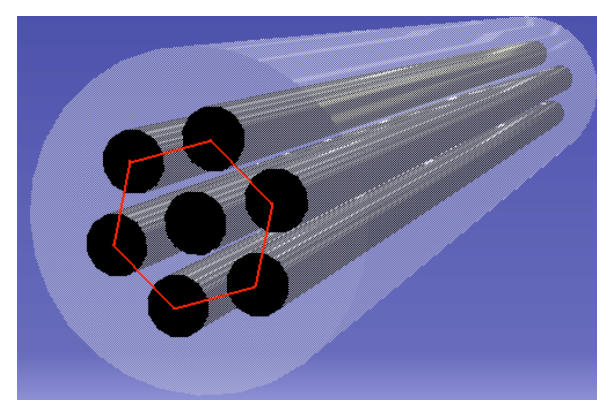
\includegraphics[scale=0.7]{Figures/cluster.eps} 
\caption{Simplified cluster geometry used for CANDU reactor cases.}\label{fig:Cluster}
  \end{center}
\end{figure}

\item[\moc{RADIUS}] keyword used to set the pin-cell radii.

\item[\dusa{r1}] real value set to the fuel pellet radius in m.

\item[\dusa{r2}] real value set to the internal clad rod radius in m.

\item[\dusa{r3}] real value set to the external clad rod radius in m.

\item[\dusa{r4}] real value set to the guide tube radius in m.

\item[\moc{POROS}] keyword used to set the oxyde porosity of fuel. Porosity affects some built-in correlations
used to represent the heat conduction phenomenon in fuel.

\item[\dusa{poros}] real value set to the oxyde porosity. The default value is 0.05.

\item[\moc{PUFR}] keyword used to set the plutonium mass enrichment of fuel. Plutonium enrichment affects some built-in correlations
used to represent the heat conduction phenomenon in fuel.

\item[\dusa{pufr}] real value set to the plutonium mass enrichment. This value can be unique or channel-dependent. The default value is 0.0.

\item[\moc{F-RUG}] keyword used to set the rugosity of the fuel rod, used in M\"uller-Steinhagen correlation for coolant friction.

\item[\dusa{epsr}] real value set to the rugosity of the fuel rod in m. The default value is 0.0.

\item[\moc{THETA}] keyword used to set the angle of the fuel channel, used in M\"uller-Steinhagen correlation for coolant friction.

\item[\dusa{theta}] real value set to the angle of the fuel channel in radians. The default value is 0.0, corresponding to a vertical channel.

\item[\moc{CONDF}] keyword used to set the fuel thermal conductivity as a function of local fuel temperature $T_{fuel}$.
Fuel conductivity is computed as

$$\lambda_{fuel} = \sum_{k=0}^{\dusa{ncond}} {\dusa{kcond}(k)*(T_{fuel})^k + \frac{\dusa{inv}}{T_{fuel}-\dusa{ref}}}$$

with $\lambda_{fuel}$ in $W/m/K$ and $T_{fuel}$ in the selected unit (Kelvin or Celsius).

By default, built-in models are used, taking into account oxyde porosity and plutonium mass enrichment.
Note that oxyde porosity and plutonium mass enrichment are ignored if this keyword is used.

\item[\dusa{ncond}] integer value set to the degree of the conductivity polynomial.

\item[\dusa{kcond}] real value set to the coefficient of the conductivity polynomial. $\dusa{ncond}+1$ coefficients are expected.

\item[\dusa{unit}] string value set to the unit of temperature $T$ in the conductivity function. Can be either \dusa{CELSIUS} or \dusa{KELVIN}.

\item[\moc{INV}] keyword used to add an inverse term in the fuel conductivity function.

\item[\dusa{inv}] real value set to the coefficient in the inverse term of fuel conductivity.
The default value is 0.0 (i.e. no inverse term).

\item[\dusa{ref}] real value set to the reference in the inverse term of fuel conductivity.

\item[\moc{CONDC}] keyword used to set the clad thermal conductivity as a function of local clad temperature $T_{clad}$.
Clad conductivity is computed with the following polynomial

$$\lambda_{clad} = \sum_{k=0}^{\dusa{ncond}} {\dusa{kcond}(k)*(T_{clad})^k}$$

with $\lambda_{clad}$ in $W/m/K$ and $T_{clad}$ in the selected unit (Kelvin or Celsius).

By default, a built-in model is used.

\item[\moc{HGAP}] keyword used to set the heat exchange coefficient of the gap as a constant.
By default, a built-in model is used.

\item[\dusa{hgap}] real value set to the constant heat exchange coefficient of the gap in $W/m^2/K$.

\item[\moc{HCONV}] keyword used to set the heat transfer coefficient between clad and fluid as a constant.
By default, this coefficient is computed using a built-in correlation.

\item[\dusa{hconv}] real value set to the constant heat transfer coefficient between clad and fluid in $W/m^2/K$.

\item[\moc{TEFF}] keyword used to set the weighting factor in the effective fuel temperature approximation.
The effective fuel temperature is used for the cross sections interpolations on fuel temperature.

\item[\dusa{wteff}] real value $W_{\rm teff}$ set to the weighting factor in the effective fuel temperature.
The effective fuel temperature is computed as

$$
T^{\rm fuel}_{\rm eff}=W_{\rm teff}*T^{\rm fuel}_{\rm surface}+(1-W_{\rm teff})*T^{\rm fuel}_{\rm center}
$$

where $0\le W_{\rm teff} \le 1$, $T^{\rm fuel}_{\rm surface}$ is the temperature at the surface of the fuel pellet (K), and $T^{\rm fuel}_{\rm center}$ is the temperature at the center of the fuel pellet (K).

By default, the Rowlands weighting factor $W_{\rm teff}={5 \over 9}$ is used\cite{Rowlands}.

\item[\moc{CONV}] keyword used to set the convergence criteria for solving the conduction and the conservation equation.

\item[\dusa{maxit1}] integer value set to the maximum number of iterations for computing the
conduction integral. The default value is 50.

\item[\dusa{maxit2}] integer value set to the maximum number of iterations for computing the
center pellet temperature. The default value is 50.

\item[\dusa{maxit3}] integer value set to the maximum number of iterations for computing the
coolant parameters (mass flux, pressure, enthalpy and density) in case of a transient calculation. The default value is 50.

\item[\dusa{ermaxt}] real value set to the maximum temperature error in K. The default value is 1~K.

\item[\dusa{ermaxc}] real value set to the maximum relative  error for parameters given by the resolution of flow conservation equations (pressure, velocity and enthalpy). The default value is $10^{-3}$.

\item[\moc{RODMESH}] keyword used to set the radial discretization of pin-cells.

\item[\dusa{nb1}] integer value set to the number of discretisation points in fuel. The default value
is 5.

\item[\dusa{nb2}] integer value set to the number of discretisation points in the whole pin-cell (fuel+cladding). The default value
is 8.

\item[\moc{FORCEAVE}] keyword used to force the use of the average approximation during the fuel conductivity evaluation.
By default, a rectangle quadrature approximation is used.

\item[\moc{MONO}] keyword used to set a one-phase flow model.

\item[\moc{BOWR}] keyword used to set a subcooling model based on the Bowring correlation\cite{bowring} (default option).

\item[\moc{SAHA}] keyword used to set a subcooling model based on the Saha-Zuber correlation\cite{lahey}. This option is recommended for BWR and CANDU applications.

\item[\moc{RAD-PROF}] keyword used to set radial power form factors. By default, these factors are set to 1.0.

\item[\dusa{rprad}] radius corresponding to a form factor with 0 $\le$ \dusa{rprad} $\le$ \dusa{r1}. This value doesn't need to correspond to a
material limit in the fuel rod.

\item[\dusa{fprad}] radial power form factor corresponding to radius \dusa{rprad}.

\item[\moc{POWER-LAW}] keyword used to define a time-dependent power law in the input. By default, the power is recovered from the fuelmap object \dusa{MAPFL}.

\item[\dusa{tpow}] total power delivered in the reactor in W.

\item[\dusa{ntime}] number of tabulation points for the power law.

\item[\dusa{t(i)}] tabulation abscissa in time (s).

\item[\dusa{pow(i)}] tabulation power factor corresponding to \dusa{t(i)}. The reactor power at time \dusa{t(i)} is given as \dusa{tpow}$\times$\dusa{pow(i)}.

\item[\moc{SET-PARAM}] keyword used to indicate the input (or modification)
of the actual values for a parameter specified using its \dusa{PNAME}.

\item[\moc{PNAME}] keyword used to specify \dusa{PNAME}.

\item[\dusa{PNAME}] \texttt{character*12} name of a parameter.

\item[\dusa{pvalue}] single real value containing the actual
parameter's values. Note that this value will not be checked for consistency
by the module. It is the user responsibility to provide the valid parameter's value
which should be consistent with those recorded in the multicompo or Saphyb database.

\item[\moc{PICK}]  keyword used to recover the temperature variation parameter $R$ in a CLE-2000 variable. This parameter describes the variation of
averaged fuel and coolant temperatures during a time step using the formula
$$ R=\max \left\{{1\over \Delta T_{\rm fuel}} \left|\bar T_{\rm fuel}(n)-\bar T_{\rm fuel}(n-1)\right|,
 {1\over \Delta T_{\rm cool}} \left|\bar T_{\rm cool}(n)-\bar T_{\rm cool}(n-1)\right| \right\}$$

\noindent where $\Delta T_{\rm fuel}=5 \ {\rm K}$ and $\Delta T_{\rm cool}=40 \ {\rm K}$.

\item[\dusa{ratio}] \texttt{character*12} CLE-2000 variable name in which the temperature variation parameter will be placed.

\end{ListeDeDescription}
\clearpage


\section{POINT KINETICS MODULES}\label{sect:modesc4}

\subsection{The \moc{PKINI:} module}\label{sect:pkini}

\vskip 0.2cm
The \moc{PKINI:} module is used to initialize the point kinetics parameters, to define the delayed neutron information
and to set the global feedback parameters. The point kinetics equations are solved for a {\sl time stage} using module
\moc{PKINS:} (See Sect.~\ref{sect:pkins}) as a function of a fixed set of global parameters recovered from the \dds{map} object \dusa{MAPFL}.
Modules \moc{PKINI:} and \moc{PKINS:} are intended to be used with thermal-hydraulics module \moc{THM:} (See Sect.~\ref{sect:thm})
to simulate a single reactor channel.

\vskip 0.08cm

\noindent
The \moc{PKINI:} module specification is:

\begin{DataStructure}{Structure \moc{PKINI:}}
\dusa{MAPFL} \moc{:=} \moc{PKINI:} \dusa{MAPFL} \moc{::} \dstr{descpkini}
\end{DataStructure}

\noindent where

\begin{ListeDeDescription}{mmmmmmmm}

\item[\dusa{MAPFL}] \texttt{character*12} name of the \dds{map} 
object containing fuel regions description and global parameter informations.

\item[\dstr{descpkini}] structure describing the input data to the \moc{PKINI:} module. 

\end{ListeDeDescription}

\vskip 0.2cm

\subsubsection{Input data to the \moc{PKINI:} module}\label{sect:pkinistr}

\begin{DataStructure}{Structure \dstr{descpkini}}
$[$ \moc{EDIT} \dusa{iprint} $]$ \\
\moc{POWER} \dusa{power} \\
$[$ \moc{EPSILON} \dusa{epsilon} $]$ \\
\moc{TIME} \dusa{t0} \dusa{dt} \\
\moc{LAMBDA} \dusa{lambda} \\
\moc{NGROUP} \dusa{ngroup} \\
\moc{BETAI} (\dusa{beta}(i),i=1,\dusa{ngroup}) \moc{LAMBDAI} (\dusa{dlambda}(i),i=1,\dusa{ngroup}) \\
\moc{ALPHA} $[[$ \dusa{PNAME} $\{$ \moc{DIRECT} $|$ \moc{DERIV} $|$ \moc{SQDERIV} $\}$ \\
~~~~$[~\{$ \moc{LINEAR} $|$ \moc{CUBIC} $\}~]$ \dusa{nalpha} (\dusa{x}(i) \dusa{y}(i),i=1,\dusa{nalpha}) $]]$ \moc{ENDA} \\
$[$ \moc{PTIME} $[[$ \dusa{PNAME} $[~\{$ \moc{LINEAR} $|$ \moc{CUBIC} $\}~]~\{$\dusa{ntime} (\dusa{t}(i) \dusa{x}(i),i=1,\dusa{ntime}) $|$ \\
~~~~\moc{T-DELT} $[$ \dusa{nxy} $]$ \dusa{t1} \dusa{t2} \moc{P-VALV} \dusa{gamma} \dusa{p1} \dusa{p2} \dusa{tb1}
\dusa{bval1} $[$ \moc{RESET} \dusa{p3} \dusa{tb2} \dusa{bval2} $]~\}~]]$ \moc{ENDP} $]$ \\
;
\end{DataStructure}

\noindent where
\begin{ListeDeDescription}{mmmmmmmm}

\item[\moc{EDIT}] keyword used to set \dusa{iprint}.

\item[\dusa{iprint}] integer index used to control the printing on screen:
= 0 for no print; = 1 for minimum printing; larger values produce
increasing amounts of output.

\item[\moc{POWER}] keyword used to set the initial reactor power.

\item[\dusa{power}] reactor power in MW.

\item[\moc{EPSILON}] keyword used to set the epsilon of the Runge-Kutta solver used to adjust the internal time step. The default value is $\epsilon=1.0\times 10^{-2}$.

\item[\dusa{epsilon}] user-selected epsilon.

\item[\moc{TIME}] keyword used to set the initial time and stage duration. It is possible to readjust the stage duration in module \moc{PKINS:}.

\item[\dusa{t0}] initial time (s).

\item[\dusa{dt}] stage duration (s).

\item[\moc{LAMBDA}] keyword used to set the prompt neutron generation time.

\item[\dusa{lambda}] prompt neutron generation time (s).

\item[\moc{NGROUP}] keyword used to set the number of delayed precursor groups.

\item[\dusa{ngroup}] number of delayed precursor groups.

\item[\moc{BETAI}] keyword used to set the delayed neutron fraction vector.

\item[\dusa{betai}] value of the delayed neutron fraction in a delayed precursor group.

\item[\moc{LAMBDAI}] keyword used to set the delayed neutron time constant vector.

\item[\dusa{lambdai}] value of the delayed neutron time constant (s) in a delayed precursor group.

\item[\moc{ALPHA}] keyword used to set the feedback parameters.

\item[\moc{PNAME}] character*12 name of a feedback parameter. A feedback parameter should be a global parameter defined in the fuelmap.

\item[\moc{DIRECT}] keyword indicating that the reactivity is a direct function of the global parameter.

\item[\moc{DERIV}] keyword indicating that the reactivity is a function of the variation of the local parameter with respect to its initial value.

\item[\moc{SQDERIV}] keyword indicating that the reactivity is a function of the variation of the square root of the local parameter with respect to its initial value.
This option is generally used to represent the Doppler effect due to the fuel temperature.

\item[\moc{LINEAR}] keyword indicating that interpolation of the reactivity effect uses linear Lagrange polynomials (default option).

\item[\moc{CUBIC}] keyword indicating that interpolation of the reactivity effect uses the Ceschino method
with cubic Hermite polynomials, as presented in Ref.~\citen{Intech2011}.

\item[\dusa{nalpha}] number of values in the table describing reactivity effects for feedback parameter \moc{PNAME}.

\item[\dusa{x}] value of the global parameter.

\item[\dusa{y}] corresponding reactivity coefficient.

\item[\moc{PTIME}] keyword used to set the time laws for some feedback parameters.

\item[\dusa{ntime}] number of values in the time law for feedback parameter \moc{PNAME}.

\item[\dusa{t}] time (s)

\item[\dusa{x}] corresponding value of the global parameter.

\item[\moc{T-DELT}] keyword used to set an analytical time law between two times.

\item[\dusa{nxy}] number of points used to construct the discrete time law. The default value is \dusa{nxy} $=1001$.

\item[\dusa{t1}] initial time (s) for the analytical time law domain.

\item[\dusa{t2}] final time (s) for the analytical time law domain.

\item[\moc{P-VALV}] keyword used to define a time law corresponding to the depressurization of a gas reservoir. The time-vatiation of the pressure $P(t)$ in a
reservoir is given by a relation of the form
\begin{equation}
P(t)=\begin{cases} P_{\rm max} & {\rm if} \ t \le {\rm \dusa{tb1}}\\
\max{\left(P_{\rm min},{\displaystyle P_{\rm max}\over\displaystyle (1+Bt)^\alpha}\right)} & {\rm otherwise}\end{cases}
\label{eq:pkin1}
\end{equation}

\noindent where $P_{\rm max}$ is the pressure of the reservoir at time $t\le$ \dusa{tb1}, before depressurization and $P_{\rm min}$ is the final pressure after
depressurization. $B$ (s$^{-1}$) is the time constant of the exhaust pipe and $\alpha$ is given by relation
\begin{equation}
\alpha={2\gamma\over \gamma-1}
\label{eq:pkin2}
\end{equation}

\noindent where $\gamma$ is a constant related to the gas capacitance ($=1.66$ for Helium).

\item[\dusa{gamma}] value of $\gamma$ parameter in Eq.~(\ref{eq:pkin2}).

\item[\dusa{p1}] value of pressure $P_{\rm max}$ in Eq.~(\ref{eq:pkin1}).

\item[\dusa{p2}] value of pressure $P_{\rm min}$ in Eq.~(\ref{eq:pkin1}).

\item[\dusa{tb1}] time (s) when the exhaust pipe is open with value \dusa{bval1}. We must have \dusa{t1}$\le$\dusa{tb1}$<$\dusa{t2}.

\item[\dusa{bval1}] value of $B$ parameter in Eq.~(\ref{eq:pkin1}) after time \dusa{tb1}.

\item[\moc{RESET}] optional keyword used to reset the opening of the exhaust pipe after a fixed period of time.

\item[\dusa{p3}] value of pressure $P_{\rm min}$ in Eq.~(\ref{eq:pkin1}) after reset.

\item[\dusa{tb2}] time (s) when the exhaust pipe is open with value \dusa{bval2}. We must have \dusa{tb1}$<$\dusa{tb2}$<$\dusa{t2}.

\item[\dusa{bval2}] value of $B$ parameter in Eq.~(\ref{eq:pkin1}) after time \dusa{tb2}.

\end{ListeDeDescription}
\clearpage

\subsection{The \moc{PKINS:} module}\label{sect:pkins}

\vskip 0.2cm
The feedback parameters are responsible for the introduction of reactivity in the solution of the point-kinetics equations.
Some feedback parameters have their time variation set by {\sl time laws} defined in module  \moc{PKINI:} (See Sect.~\ref{sect:pkini}).
Some other are assumed constant during a {\sl time stage}, corresponding to a single call to module \moc{PKINS:}. The \moc{PKINS:}
module is used to solve the point-kinetics equations over a single time stage.

\vskip 0.08cm

\noindent
The \moc{PKINS:} module specification is:

\begin{DataStructure}{Structure \moc{PKINS:}}
$[$ \dusa{MAPFL} \moc{:=} $]$ \moc{PKINS:} \dusa{MAPFL} \moc{::} \dstr{descpkins}
\end{DataStructure}

\noindent where

\begin{ListeDeDescription}{mmmmmmmm}

\item[\dusa{MAPFL}] \texttt{character*12} name of the \dds{map} 
object containing fuel regions description and global parameter informations. This object is declared
in read-only mode if and only if keyword \moc{PICKR} is set.

\item[\dstr{descpkins}] structure describing the input data to the \moc{PKINS:} module. 

\end{ListeDeDescription}

\vskip 0.2cm

\subsubsection{Input data to the \moc{PKINS:} module}\label{sect:pkinsstr}

\begin{DataStructure}{Structure \dstr{descpkins}}
$[$ \moc{EDIT} \dusa{iprint} $]$ \\
\moc{TIME} \dusa{t0} \dusa{dt} \\
$\{~[$ \moc{POWER} \dusa{power} $|$ \moc{Y-INIT} (\dusa{y}(i),i=1,\dusa{ngroup+1}) $\}~]$ \\
$[~\{$ \moc{PICK}  {\tt >>} \dusa{power\_out} {\tt <<} $|$ \moc{PICKR}  {\tt >>} \dusa{rho} {\tt <<} $\}~]$ \\
;
\end{DataStructure}

\noindent where
\begin{ListeDeDescription}{mmmmmmmm}

\item[\moc{EDIT}] keyword used to set \dusa{iprint}.

\item[\dusa{iprint}] integer index used to control the printing on screen:
= 0 for no print; = 1 for minimum printing; larger values produce
increasing amounts of output.

\item[\moc{TIME}] keyword used to set the beginning-of-stage and duration times.

\item[\dusa{t0}] beginning-of-stage time (s).

\item[\dusa{dt}] stage duration (s). \dusa{dt} $=0.0$ if keyword \moc{PICKR} is set.

\item[\moc{POWER}] keyword used to set the beginning-of-stage reactor power.

\item[\dusa{power}] beginning-of-stage reactor power in MW.

\item[\moc{Y-INIT}] keyword used to set the beginning-of-stage solution of the point kinetics equations.

\item[\dusa{y}] beginning-of-stage value of a component of the beginning-of-stage solution. \dusa{ngroup} is the
number of delayed precursor groups.

\item[\moc{PICK}]  keyword used to recover the end-of-stage power (in MW) in a CLE-2000 variable.

\item[\dusa{power\_out}] \texttt{character*12} CLE-2000 variable name in which the extracted power value will be placed.

\item[\moc{PICKR}]  keyword used to recover the reactivity at time \dusa{t0} in a CLE-2000 variable.

\item[\dusa{rho}] \texttt{character*12} CLE-2000 variable name in which the reactivity value will be placed.

\end{ListeDeDescription}
\clearpage


\section{OPTIMIZATION MODULES}\label{sect:modesc5}

This section is related to optimization capabilities available in Donjon and
based on generalized perturbation theory.\cite{optex1,optex2} General information
about the generalized perturbation theory can be found in Sect. 5.3 of Ref.~\citen{PIP2016}.

\subsection{The {\tt DLEAK:} module}

The {\tt DLEAK:} module is used to create a delta {\sc macrolib} (type {\tt L\_MACROLIB}) with respect to leakage information.
Derivatives of leakage-related information (recovered from the input {\sc macrolib}) are stored in the {\tt STEP} heteroneneous list components
present in the output {\sc macrolib}. Derivatives can be taken with respect to a leakage parameter itself
($D_{g,i}$ or $\Sigma_{1,g,i}$) or relative to factor $\mu$ in $\mu D_{g,i}$ or $\mu\Sigma_{1,g,i}$. Note that factor $\mu$ is not a
SPH factor because it multiplies only leakage-related parameters. One component of the
{\tt STEP} heteroneneous list is created for each value of energy group $g$ and for each value of mixture $i$.

\vskip 0.08cm

The calling specifications are:

\begin{DataStructure}{Structure \dstr{DLEAK:}}
\dusa{DMACRO} \dusa{OPTIM} \moc{:=} \moc{DLEAK:} \dusa{MACRO} \moc{::} \dstr{dleak\_data}
\end{DataStructure}

\goodbreak
\noindent where

\begin{ListeDeDescription}{mmmmmm}

\item[\dusa{DMACRO}] {\tt character*12} name of a {\sc lcm} object (type {\tt L\_MACROLIB}) containing the delta {\sc macrolib}
information. \dusa{DMACRO} is created by the module. A {\tt STEP} heteroneneous list is present in \dusa{DMACRO}.

\item[\dusa{OPTIM}] {\tt character*12} name of a second {\sc lcm} object (type {\tt L\_OPTIMIZE}) created by the module. Leakage-related parameters are saved
in the the control variable record {\tt 'VAR-VALUE'} of \dusa{OPTIM} object. Input data defined in Sect.~\ref{sect:dleak_data} is
also saved in \dusa{OPTIM} object.

\item[\dusa{MACRO}] {\tt character*12} name of the {\sc lcm} object (type {\tt L\_MACROLIB}) containing the input {\sc macrolib}.

\item[\dstr{dleak\_data}] structure containing the data to module {\tt DLEAK:} (see Sect.~\ref{sect:dleak_data}).

\end{ListeDeDescription}

\vskip 0.2cm

\subsubsection{Data input for module {\tt DLEAK:}}\label{sect:dleak_data}

\begin{DataStructure}{Structure \dstr{dleak\_data}}
$[$ \moc{EDIT} \dusa{iprint} $]$ \\
\moc{TYPE} $\{$ \moc{DIFF} $|$ \moc{NTOT1} $\}$ \\
\moc{DELTA} $\{$ \moc{VALUE} $|$ \moc{FACTOR} $\}$ \\
$[$ \moc{MIXMIN} \dusa{ibm1} $]~[$ \moc{MIXMAX} \dusa{ibm2} $]$\\
$[$ \moc{GRPMIN} \dusa{ngr1} $]~[$ \moc{GRPMAX} \dusa{ngr2} $]$\\
;
\end{DataStructure}

\noindent where
\begin{ListeDeDescription}{mmmmmm}

\item[\moc{EDIT}] keyword used to set \dusa{iprint}.

\item[\dusa{iprint}] index used to control the printing in module {\tt DLEAK:}.

\item[\moc{TYPE}] keyword used to set the leakage parameter that is differentiated.

\item[\moc{DIFF}] differentiation with respect to diffusion coefficients.

\item[\moc{NTOT1}] differentiation with respect to $P_1$-weighted macroscopic total cross sections.

\item[\moc{DELTA}] keyword used to set the type of differentiation.

\item[\moc{VALUE}] differentiation with respect to the leakage parameter itself.

\item[\moc{FACTOR}] differentiation with respect to the correction factor $\mu$.

\item[\moc{MIXMIN}] keyword used to set the first mixture where leakage parameters are differentiated. By default,
the first mixture index is used.

\item[\dusa{ibm1}] minimum mixture index where leakage parameters are differentiated.

\item[\moc{MIXMAX}] keyword used to set the last mixture where leakage parameters are differentiated. By default,
the total number of mixtures in \dusa{MACRO} is used.

\item[\dusa{ibm2}] maximum mixture index where leakage parameters are differentiated.

\item[\moc{GRPMIN}] keyword used to set the first energy group where leakage parameters are differentiated. By default,
the first energy group index is used.

\item[\dusa{ngr1}] minimum energy group index where leakage parameters are differentiated.

\item[\moc{GRPMAX}] keyword used to set the last energy group where leakage parameters are differentiated. By default,
the total number of energy groups in \dusa{MACRO} is used.

\item[\dusa{ngr2}] maximum energy group index where leakage parameters are differentiated.

\end{ListeDeDescription}
\clearpage

\vskip 1.0cm
\subsection{The {\tt DSPH:} module}

The {\tt DSPH:} module is used to create a delta {\sc macrolib} (type {\tt L\_MACROLIB}) with respect to SPH factor variation.
Derivatives of diffusion coefficient and cross-section information (recovered from the input {\sc macrolib}) are stored in the {\tt STEP} heteroneneous list components
present in the output {\sc macrolib}. One component of the {\tt STEP} heteroneneous list is created for each value of energy group $g$ and for each value of mixture $i$.

\vskip 0.08cm

The calling specifications are:

\begin{DataStructure}{Structure \dstr{DSPH:}}
\dusa{DMACRO} \dusa{OPTIM} \moc{:=} \moc{DSPH:} \dusa{MACRO} \moc{::} \dstr{dsph\_data}
\end{DataStructure}

\goodbreak
\noindent where

\begin{ListeDeDescription}{mmmmmm}

\item[\dusa{DMACRO}] {\tt character*12} name of a {\sc lcm} object (type {\tt L\_MACROLIB}) containing the delta {\sc macrolib}
information. \dusa{DMACRO} is created by the module. A {\tt STEP} heteroneneous list is present in \dusa{DMACRO}.

\item[\dusa{OPTIM}] {\tt character*12} name of a second {\sc lcm} object (type {\tt L\_OPTIMIZE}) created by the module. SPH factors are saved
in the the control variable record {\tt 'VAR-VALUE'} of \dusa{OPTIM} object. Input data defined in Sect.~\ref{sect:dsph_data} is
also saved in \dusa{OPTIM} object.

\item[\dusa{MACRO}] {\tt character*12} name of the {\sc lcm} object (type {\tt L\_MACROLIB}) containing the input {\sc macrolib}.

\item[\dstr{dsph\_data}] structure containing the data to module {\tt DSPH:} (see Sect.~\ref{sect:dsph_data}).

\end{ListeDeDescription}

\vskip 0.2cm

\subsubsection{Data input for module {\tt DSPH:}}\label{sect:dsph_data}

\begin{DataStructure}{Structure \dstr{dsph\_data}}
$[$ \moc{EDIT} \dusa{iprint} $]$ \\
$[~$\moc{SPH} $\{$ \moc{PN} $|$ \moc{SN} $|$ \moc{ALBEDO} $\}~]$ \\
$[$ \moc{GRPMIN} \dusa{ngr1} $]~[$ \moc{GRPMAX} \dusa{ngr2} $]$\\
;
\end{DataStructure}

\noindent where
\begin{ListeDeDescription}{mmmmmm}

\item[\moc{EDIT}] keyword used to set \dusa{iprint}.

\item[\dusa{iprint}] index used to control the printing in module {\tt DSPH:}.

\item[\moc{PN}] keyword to activate the calculation of heterogeneous SPH factors of diffusion, PN or SPN type.

\item[\moc{SN}] keyword to activate the calculation of heterogeneous SPH factors of PIJ, IC, SN or MOC type.
This is the default option.

\item[\moc{ALBEDO}] keyword to activate the calculation of a unique SPH factor assigned to the albedo function
in each energy group.

\item[\moc{GRPMIN}] keyword used to set the first energy group where SPH correction is applied. By default,
the first energy group index is used.

\item[\dusa{ngr1}] minimum energy group index where SPH correction is applied.

\item[\moc{GRPMAX}] keyword used to set the last energy group where SPH correction is applied. By default,
the total number of energy groups in \dusa{MACRO} is used.

\item[\dusa{ngr2}] maximum energy group index where SPH correction is applied.

\end{ListeDeDescription}
\clearpage

\vskip 1.0cm
\subsection{The {\tt DREF:} module}\label{sect:DREFData}

This module is used to set fixed sources that can be used in the right hand term of an adjoint
fixed source eigenvalue problem. This type of equation appears in generalized perturbation theory (GPT) applications.
The fixed sources set in {\tt DREF:} are corresponding to the gradient of the RMS functional which is a measure of
the discrepancy between actual and reference (or target) reaction rate distributions. The actual reaction rate distribution
is recovered from a \dusa{MICRO} or \dusa{MACRO} object. The reference reaction rate distribution is recovered from 
a \dusa{MICREF} or \dusa{MACREF} object.

\subsubsection{Minimizing the RMS error of power distribution}

The fixed sources are computed for the case where the \dds{optimize} object was initialized in module {\tt DLEAK:}. This option is used with the {\sl OPTEX
reflector model}.\cite{optex3}

Actual power values are defined as
$$
P_i\{\bff(\phi)(r)\}\equiv \left< H , \phi \right>_i=\int_0^\infty dE \int_{V_i} d^3r \, H(\bff(r),E) \, \phi(\bff(r),E)
$$

\noindent where the power factors $H(\bff(r),E)$ and fluxes $\phi(\bff(r),E)$ are recovered from {\tt H-FACTOR} and 
{\tt FLUX-INTG} records in a {\sc macrolib} object.

\vskip 0.08cm

The RMS error on power distribution is an homogeneous functional of the flux defined as
$$
{\cal F}\{\bff(\phi)(r)\}=\sum_i \left({\left< H , \phi \right>_i\over \left< H , \phi \right>} - {P^*_i\over \sum_j P^*_j} \right)^2
$$
\noindent where the reference (or target) powers $P^*_i$ are obtained from the full-core reference transport calculation.

\vskip 0.08cm

The gradient of functional ${\cal F}\{\bff(\phi)(r)\}$ is a $G$-group function of space defined as
\begin{align*}
\bff(\nabla){\cal F}\{\bff(\phi)(\zeta);\bff(r)\}={2\over \left< H , \phi \right>} \sum_i  \left({\left< H , \phi \right>_i\over \left< H , \phi \right>} -
{P^*_i\over \sum_j P^*_j}\right)\left( \delta_i(\bff(r))-{\left< H , \phi \right>_i\over \left< H , \phi \right>} \right) \left[\begin{matrix}H_1(\bff(r))\cr H_2(\bff(r)) \cr \vdots \cr H_G(\bff(r)) \end{matrix}\right]
\end{align*}

\noindent where $\delta_i(\bff(r))=1$ if $\bff(r) \in V_i$ and $=0$ otherwise.

\vskip 0.08cm

Each fixed source $\bff(\nabla){\cal F}\{\bff(\phi)(\zeta);\bff(r)\}$ is orthogonal to the flux $\bff(\phi)(\bff(r))$.

\subsubsection{Minimizing the RMS error associated with SPH factor calculation}\label{sect:sph_newton}

The fixed sources are computed for the case where the \dds{optimize} object was initialized in module {\tt DSPH:}. Module
{\tt DREF} is call to compute the gradients required for computing SPH factors using an optimization algorithm (OPTEX in
{\tt PLQ:}, quasi-Newton in {\tt LNSR:}, Newton in {\tt FPSPH:}). Module {\tt DREF} computes the direct gradients and the
fixed sources to be used in a fixed-source eigenvalue problem originating from the generalized perturbation theory (GPT).

\vskip 0.08cm

Fundamental mode conditions are the cases where no neutron is leaking due to the boundary conditions. In the case where the macro-calculation over macro-group $g$ is done
in non-fundamental mode conditions, it is proposed to apply a SPH correction
on the {\sl albedo functions} corresponding to boundaries with a non-conservative condition in the reference calculation.\cite{sph2019} If the macro calculation is performed in diffusion
or $P_1$ approximation, the albedo function $\Lambda(\beta_g)$ corresponding to a non-conservative boundary is defined as
\begin{equation}
\Lambda(\beta_g)={1\over 2}{1-\beta_g \over 1+\beta_g}
\label{eq:eq1.6}
\end{equation}
\noindent where $\beta_g$ is the albedo in macro-group $g$. The net current $\bff(J)_g(\bff(r))$ escaping the domain at point $\bff(r)$ of the boundary is given by the {\sl albedo boundary condition} as
\begin{equation}
-\bff(J)_g(\bff(r))\cdot\bff(N)(\bff(r))+\Lambda(\beta_g) \, \phi_g(\bff(r))=0 \ \ \ \ {\rm if} \ \bff(r) \in \partial V
\label{eq:eq1.7}
\end{equation}

\noindent where $\partial V$ is the fraction of the domain where the non-conservative boundary condition is applied and $\bff(N)(\bff(r))$ is the outgoing normal unit vector.

\vskip 0.08cm

The integrated flux are defined over the macro-region $m$ and macro-group $g$ as
\begin{equation}
F_{m,g}\equiv \left< \phi \right>_{m,g}=\int_{V_m} d^3r \, \phi_g(\bff(r))
\label{eq:eq1.7a}
\end{equation}

\vskip 0.08cm

The net leakage $L_{g}$ over each macro group due to non conservative boundary conditions is defined as
\begin{equation}
L_{g}\equiv \left< \Lambda\phi\right>_g= \int_{\partial V} d^2r \, \Lambda(\beta_g) \, \phi_g(\bff(r)) =\int_{\partial V} d^2r \,\bff(J)_g(\bff(r))\cdot \bff(N)(\bff(r))\ .
\label{eq:eq1.8}
\end{equation}

\vskip 0.08cm

In order to preserve the neutron balance in macro-group $g$, cross section data and albedo functions must all be SPH corrected. The correction specific to albedo functions is written
\begin{equation}
\tilde\Lambda_g=\mu_{M+1,g}\, \Lambda^*_g
\label{eq:eq1.9}
\end{equation}
\noindent where $M$ is the total number of macro-regions and $\Lambda^*_g$ is the albedo function of the reference calculation in macro-group $g$. This
correction technique is proposed as an alternative to the discontinuity factor correction used by Ref. \citen{inl}.

\vskip 0.08cm

In fundamental mode conditions and in cases where Eq.~(\ref{eq:eq1.9}) is used, an infinity of
SPH factor sets can satisfy the reference reaction rates in each macro-group $g$.
A unique set is selected with the application of an arbitrary normalization condition. The simplest option is to use the {\sl flux-volume normalization condition} which consists to preserve the averaged flux
in the lattice. This normalization condition, satisfied in each macro-group $g$, is written
\begin{equation}
\sum_{m=1}^M \int_{V_m} d^3r \ \widetilde\phi_{g}(\bff(r))=\sum_{m=1}^M F_{m,g}^{*} \ , \ \ g \le G
\label{eq:eq1.10}
\end{equation}
\noindent where $F_{m,g}^{*}$ is the volume-integrated flux in macro-region $V_m$ and macro-group $g$ of the reference calculation.

\vskip 0.08cm

Equation~(\ref{eq:eq1.10}) can be rewritten as
\begin{equation}
\sum_{m=1}^M {F_{m,g}^{*}\over \mu_{m,g}}=\sum_{m=1}^M F_{m,g}^{*}  \ , \ \ g \le G .
\label{eq:eq1.11}
\end{equation}

The absorption rates are defined over the macro-region $m$ and macro-group $g$ as
\begin{equation}
P_{{\rm a},m,g}\equiv \left< \Sigma_{\rm a} , \phi \right>_{m,g}=\int_{V_m} d^3r \, \Sigma_{{\rm a},g}(\bff(r)) \, \phi_g(\bff(r))
\label{eq:eq2.2}
\end{equation}
\noindent where $i\le I$ and $g\le G$ and where

\begin{equation}
\Sigma_{{\rm a},g}(\bff(r))=\Sigma_g(\bff(r))-\Sigma_{{\rm s},g}(\bff(r)) .
\label{eq:eq2.3}
\end{equation}

\vskip 0.08cm

The $\nu$-fission rates are defined over the macro-region $m$ and macro-group $g$ as
\begin{equation}
P_{{\rm f},m,g}\equiv \left< \nu\Sigma_{\rm f} , \phi \right>_{m,g}=\int_{V_m} d^3r \, \nu\Sigma_{{\rm f},g}(\bff(r)) \, \phi_g(\bff(r))
\label{eq:eq2.2b}
\end{equation}
\noindent where $i\le I$ and $g\le G$ and where $\nu\Sigma_{{\rm f},g}(\bff(r))$ is the macroscopic fission cross section multiplied by the averaged number of neutrons emitted per fission.

\vskip 0.08cm

The absorption and $\nu$-fission  cross sections are corrected according to
\begin{equation}
\Sigma_{{\rm a},m,g}=\mu_{m,g}\, \Sigma^*_{{\rm a},m,g} =\mu_{m,g}\, {P^*_{{\rm a},m,g} \over F^*_{m,g}}
\label{eq:eq2.4}
\end{equation}

\noindent and
\begin{equation}
\nu\Sigma_{{\rm f},m,g}=\mu_{m,g}\, \nu\Sigma^*_{{\rm f},m,g} =\mu_{m,g}\, {P^*_{{\rm f},m,g} \over F^*_{m,g}}
\label{eq:eq2.4b}
\end{equation}

\noindent where the reference integrated fluxes $F^*_{m,g}$ are also obtained from the full-core reference transport calculation. The SPH factors are normalized in each macro energy group
according to
\begin{equation}
\sum_{j=1}^M{F^*_{j,g} \over \mu_{j,g}} = \sum_j F^*_{j,g}  \ , \ \ g \le G .
\label{eq:eq2.5}
\end{equation}

\vskip 0.08cm

The RMS error on absorption distribution is an homogeneous functional of the flux defined as
\begin{equation}
{\cal F}\{\bff(\phi)(\bff(r))\}=\sum_{m=1}^{M+2} \sum_{g=1}^G \left( f_{m,g}\{\bff(\phi)(\bff(r))\} \right)^2
\label{eq:eq2.6}
\end{equation}
\noindent where the components $f_{m,g}\{\bff(\phi)(\bff(r))\}$ are the $M+2$ conditions to satisfy in each macro-group. They are defined as
\begin{equation}
f_{m,g}\{\bff(\phi)(\bff(r))\}=\begin{cases} {{\displaystyle \left< \Sigma_{\rm a} , \phi \right>_{m,g}\over\displaystyle  \left< \Sigma_{\rm a} , \phi \right>} {\displaystyle P^*_{{\rm a},{\rm tot}}\over \displaystyle  \Delta_{{\rm a},m,g} } - {\displaystyle  P^*_{{\rm a},m,g} \over \displaystyle \Delta_{{\rm a},m,g} }} & \text{if $m\le M$} \\
\sqrt{M}\left( {\displaystyle \left<\Lambda+\Sigma_{\rm a} , \phi\right>_g\over\displaystyle  \left< \nu\Sigma_{\rm f} ,\phi \right>} {\displaystyle P^*_{{\rm f},{\rm tot}}\over\displaystyle  \Delta_{{\rm L},g} } - {\displaystyle L^*_{g}+P^*_{{\rm a},g} \over\displaystyle  \Delta_{{\rm L},g}}\right) & \text{if $m = M+1$} \\
{\displaystyle 1\over \displaystyle F^*_g}\sum\limits_{j=1}^M {\displaystyle F^*_{j,g} \over \displaystyle \mu_{j,g}} - 1  & \text{if $m= M+2$} \end{cases} 
\label{eq:eq2.7}
\end{equation}

\noindent with
\begin{description}
\item[$P^*_{{\rm a},m,g}=$] reference (or target) absorption rates obtained from the full-core reference transport calculation
\item[$P^*_{{\rm f},m,g}=$] reference (or target) $\nu$-fission rates obtained from the full-core reference transport calculation
\item[$\Delta_{{\rm a},m,g}=$] low limit absorption rates defined as $\max \left( 10^{-4} P^*_{{\rm a},{\rm tot}},P^*_{{\rm a},m,g}\right)$ in order to avoid
division by small numbers.
\item[$L^*_{g}=$] reference leakage in macro-group $g$
\item[$\Lambda(\bff(r))=$] albedo function defined on the non-conservative boundaries $\partial V$ of the domain
\item[$\Delta_{{\rm L},g}=$] low limit leakage defined as $\max \left( 10^{-4} P^*_{{\rm f},{\rm tot}},L^*_{g}+P^*_{{\rm a},g} \right)$ in order to avoid
division by small numbers.
\end{description}

\noindent and where $P^*_{{\rm a},g}=\sum_m P^*_{{\rm a},m,g}$, $P^*_{{\rm a},{\rm tot}}=\sum_g P^*_{{\rm a},g}$, $P^*_{{\rm f},{\rm tot}}=\sum_m \sum_g P^*_{{\rm f},m,g}$ and $F^*_g=\sum_m F^*_{m,g}$.

\vskip 0.08cm

The condition $m=M+1$ in 
Eq.~(\ref{eq:eq2.7}) is based on the preservation of the effective multiplication factor of the core. The SPH normalization relations~(\ref{eq:eq1.11}) are
included in the RMS error in order to simplify the optimization process.

\vskip 0.08cm

The gradient of functional~(\ref{eq:eq2.6}) with respect to a variation of flux $\phi$ is a $G$-group function of space whose components are defined as
\begin{equation}
\nabla {\cal F}_g\{\bff(\phi)(\bff(\zeta));\bff(r)\}=\left[ {d\over d\epsilon}{\cal F}\{\bff(\phi)(\bff(\zeta))+\epsilon \, \bff(\delta)_g(\bff(\zeta)-\bff(r))\}\right]_{\epsilon=0} ; \ \ g=1,G
\label{eq:eq2.7a}
\end{equation}
\noindent where $\bff(\delta)_g(\bff(\zeta)-\bff(r))$ is a multidimensional Dirac delta distribution defined as
\begin{equation}
\bff(\delta)_g(\bff(\zeta)-\bff(r))={\rm col} \left[\delta_{g,h} \, \delta(\bff(\zeta)-\bff(r)) \, , \, h=1,G \right]
\label{eq:eq2.7b}
\end{equation}
\noindent where $\delta_{g,h}$ is a Kronecker delta function and $\delta(\bff(\zeta)-\bff(r))$ is the classical Dirac delta distribution.

\vskip 0.08cm
Next, we evaluate the gradient of each component $f_{m,g}\{\bff(\phi)(\bff(r))\}$ with respect to the SPH factors and we construct a rectangular matrix $\shadowA$, of size $(M+2)G\times (M+1)G$, defined as
\begin{equation}
\shadowA=\left\{ {\partial f_{m,g}\over \partial \mu_{n,h}}  ; \ \ m\le M+2, \ n \le M+1, \ g\le G, \ h\le G \right\} .
\label{eq:eq2.8}
\end{equation}

\vskip 0.08cm

We first evaluate the direct contribution of these derivatives for a variation of the SPH factors assigned to cross sections (i.e., for $n\le M$). Direct contributions are the chain rule terms not involving a variation in flux. These direct
gradients are
\begin{equation}
\left.{\partial f_{m,g}\over \partial \mu_{n,h}}\right|^{\rm direct} \negthinspace\negthinspace ={\left< \Sigma_{\rm a} , \phi \right>_{m,g}\over \mu_{n,h} \left< \Sigma_{\rm a} , \phi \right>} {P^*_{{\rm a},{\rm tot}}\over \Delta_{{\rm a},m,g} } \left( \delta_{m,n}\delta_{g,h}-{\left< \Sigma_{\rm a} , \phi \right>_{n,h}\over \left< \Sigma_{\rm a} , \phi \right>} \right) \ \ {\rm if} \ m\le M
\label{eq:eq2.9}
\end{equation}

\begin{equation}
\left.{\partial f_{M+1,g}\over \partial \mu_{n,h}}\right|^{\rm direct} \negthinspace\negthinspace =   { \sqrt{M} \over  \mu_{n,h}  \left< \nu\Sigma_{\rm f},\phi\right>}  {P^*_{{\rm f},{\rm tot}}\over  \Delta_{{\rm L},g} } 
\left( \delta_{g,h}\left<\Sigma_{\rm a} ,\phi\right>_{n,h}-\left<\Lambda+\Sigma_{\rm a}  ,\phi\right>_g {\left< \nu\Sigma_{\rm f} ,\phi \right>_{n,h} \over  \left< \nu\Sigma_{\rm f},\phi\right>}\right)
\label{eq:eq2.10}
\end{equation}

\noindent and
\begin{equation}
\left.{\partial f_{M+2,g}\over \partial \mu_{n,h}}\right|^{\rm direct} \negthinspace\negthinspace = -\delta_{g,h}\, {F^*_{n,g} \over \mu_{n,g}^2 F^*_g} .
\label{eq:eq2.11}
\end{equation}

\vskip 0.08cm

The SPH factors assigned to the albedo functions are not responsible for any direct contributions to the derivatives of component $f_{m,g}\{\bff(\phi)(\bff(r))\}$. Consequently,
\begin{equation}
\left.{\partial f_{m,g}\over \partial \mu_{M+1,h}}\right|^{\rm direct}=0 .
\label{eq:eq2.11a}
\end{equation}

\vskip 0.08cm

The indirect gradient of each component $f_{m,g}\{\bff(\phi)(\bff(r))\}$ with respect to the SPH factors are an effect of {\sl flux variation} and are obtained using {\sl generalized perturbation theory} (GPT). The gradient of functional $f_{m,g}\{\bff(\phi)(\bff(r))\}$ with respect to a variation of flux is a $G$-group function of space defined as
\begin{equation}
\bff(\nabla)f_{m,g}\{\bff(\phi)(\bff(\zeta));\bff(r)\}=\left[\begin{matrix}f_{m,g,1}\{\bff(\phi)(\bff(\zeta));\bff(r)\} \cr f_{m,g,2}\{\bff(\phi)(\bff(\zeta));\bff(r)\}  \cr \vdots\cr f_{m,g,G}\{\bff(\phi)(\bff(\zeta));\bff(r)\} \end{matrix}\right]
\label{eq:eq2.12}
\end{equation}

\noindent where the group-$h$ components are
\begin{equation}
\nabla f_{m,g,h}\{\bff(\phi)(\bff(\zeta));\bff(r)\} = {\Sigma_{{\rm a},h}(\bff(r))\over \left< \Sigma_{\rm a} , \phi \right>} {P^*_{{\rm a},{\rm tot}}\over \Delta_{{\rm a},m,g} } \left( \delta_m(\bff(r)) \, \delta_{g,h}-
{\left< \Sigma_{\rm a} , \phi \right>_{m,g}\over \left< \Sigma_{\rm a} , \phi \right>} \right) \ \ {\rm if} \ m\le M
\label{eq:eq2.13}
\end{equation}
\noindent where $\delta_m(\bff(r))=1$ if $\bff(r) \in V_m$ and $=0$ otherwise,

\begin{eqnarray}
\nonumber \nabla f_{M+1,g,h}\{\bff(\phi)(\bff(\zeta));\bff(r)\} \negthinspace &=& \negthinspace { \sqrt{M} \over \left< \nu\Sigma_{\rm f} , \phi \right>} {P^*_{{\rm f},{\rm tot}}\over \Delta_{{\rm L},g} } \bigg[ \left(\Lambda_{h}(\bff(r))+\Sigma_{{\rm a},h}(\bff(r))\right) \, \delta_{g,h} \\
&-& \negthinspace \nu\Sigma_{{\rm f},h}(\bff(r))\, {\left< \Lambda+\Sigma_{\rm a} , \phi \right>_{g}\over \left< \nu\Sigma_{\rm f} , \phi \right>} \bigg]
\label{eq:eq2.14}
\end{eqnarray}

\noindent and
\begin{equation}
\nabla f_{M+2,g,h}\{\bff(\phi)(\bff(\zeta));\bff(r)\} = 0 .
\label{eq:eq2.15}
\end{equation}

\vskip 0.08cm

We first compute the gradient $\bff(g)$ of the RMS error with respect to a variation of the SPH factors. We define three column vectors as
\begin{equation}
\bff(f)={\rm col} \left\{ f_{m,g}\{\bff(\phi)(\bff(r))\} \ ; \ \ m\le M+2, \ g\le G \right\} ,
\label{eq:eq2.16}
\end{equation}

\begin{equation}
\bff(\nabla)\bff(f)={\rm col} \left\{ \bff(\nabla)f_{m,g}\{\bff(\phi)(\bff(\zeta));\bff(r)\} \ ; \ \ m\le M+2, \ g\le G \right\} 
\label{eq:eq2.17}
\end{equation}

\noindent and
\begin{equation}
\bff(g)={\rm col} \left\{ {\partial {\cal F}\{\bff(\phi)(\bff(r))\} \over \partial \mu_{n,h}} ; \ \ n\le M+1, \ h\le G \right\} .
\label{eq:eq2.18}
\end{equation}

\vskip 0.08cm

From Eqs.~(\ref{eq:eq2.6}) and~(\ref{eq:eq2.7a}), we have
\begin{equation}
{\cal F}\{\bff(\phi)(\bff(r))\}=\bff(f)^\top \bff(f)
\label{eq:eq2.19}
\end{equation}

\noindent and
\begin{equation}
\bff(\nabla){\cal F}\{\bff(\phi)(\bff(\zeta));\bff(r)\}=2\bff(f)^\top \bff(\nabla)\bff(f)
\label{eq:eq2.20}
\end{equation}

\noindent so that
\begin{equation}
{\partial {\cal F} \over \partial \mu_{n,h}} =2\sum_{m=1}^{M+2} \sum_{g=1}^G  f_{m,g}\,  {\partial  f_{m,g} \over  \partial \mu_{n,h}}
\label{eq:eq2.21}
\end{equation}

\noindent where the derivatives of $f_{m,g}$ are computed taking into account both direct and indirect contributions:
\begin{equation}
{\partial  f_{m,g} \over  \partial \mu_{n,h}}=\left.{\partial  f_{m,g} \over  \partial \mu_{n,h}}\right|^{\rm direct}+\left< \bff(\nabla) f_{m,g}\{\bff(\phi)(\bff(\zeta));\bff(r)\},{\partial\over \partial\mu_{n,h}}\bff(\phi)(\bff(r))\right>
\label{eq:eq2.22}
\end{equation}

\noindent and where the bracket stands for a summation over the $G$ energy groups and an integration over the domain. The flux derivatives $\partial\bff(\phi) / \partial\mu_{n,h}$ are $G$-group functions obtained using generalized perturbation theory.

\vskip 0.08cm

Equation~(\ref{eq:eq2.21}) can be rewritten in matrix form as
\begin{equation}
\bff(g)=2 \shadowA^\top \bff(f) .
\label{eq:eq2.23}
\end{equation}

\vskip 0.08cm

The bracket term in Eq.~(\ref{eq:eq2.22}) is computed by module {\tt GRAD:}, outside module {\tt DREF:}. Module
{\tt GRAD:} compute only the {\sl direct contributions} of the gradients:
\begin{itemize}
\item By default, the objective function ${\cal F}\{\bff(\phi)(\bff(r))\}$ and direct components of vector $\bff(g)$ are computed.
\item If keyword {\tt NEWTON} is set, individual components $f_{m,g}\{\bff(\phi)(\bff(r))\}$ and direct components of matrix $\shadowA$ are computed.
\end{itemize}

\subsubsection{Calling specifications}

The calling specifications for module {\tt DREF:} are:

\begin{DataStructure}{Structure \dstr{DREF:}}
\dusa{SOURCE}~\dusa{OPTIM}~\moc{:=}~\moc{DREF:}~\dusa{OPTIM}~\dusa{FLUX}~\dusa{TRACK}~$\{$~\dusa{MICRO}~$|$~\dusa{MACRO}~$\}$ \\
~~~~~~$\{$~\dusa{MICREF}~$|$~\dusa{MACREF}~$\}$ \\
~~~~~~$[$ \moc{::}~$[$ \moc{EDIT}~\dusa{iprint} $]~[$ \moc{NODERIV} $]~[$ \moc{NEWTON} $]~[$ \moc{RMS} {\tt>>}\dusa{RMS\_VAL}{\tt <<}~$]~~]$~;
\end{DataStructure}

\noindent where
\begin{ListeDeDescription}{mmmmmmm}

\item[\dusa{SOURCE}] {\tt character*12} name of a {\sc fixed sources} (type {\tt L\_SOURCE}) object open in creation
mode. This object contains the adjoint fixed source corresponding to the RMS error on power distribution.

\item[\dusa{OPTIM}] \texttt{character*12} name of the \dds{optimize} object ({\tt L\_OPTIMIZE} signature) containing the
optimization informations. Object \dusa{OPTIM} must appear on both LHS and RHS to be able to update the previous values.

\item[\dusa{FLUX}] {\tt character*12} name of the actual {\sc flux} (type {\tt L\_FLUX}) object open in read-only mode.

\item[\dusa{TRACK}] {\tt character*12} name of the actual {\sc tracking} (type {\tt L\_TRACK}) object open in read-only mode.

\item[\dusa{MICRO}] {\tt character*12} name of the actual {\sc microlib} (type {\tt L\_LIBRARY}) object open in read-only mode. The information on
the embedded macrolib is used.

\item[\dusa{MACRO}] {\tt character*12} name of the actual {\sc macrolib} (type {\tt L\_MACROLIB}) object open in read-only mode.

\item[\dusa{MICREF}] {\tt character*12} name of reference (or target) {\sc microlib} (type {\tt L\_LIBRARY}) object open in read-only mode. The
information contained in the embedded macrolib is used to compute $P^*_i$ values.

\item[\dusa{MACREF}] {\tt character*12} name of reference (or target) {\sc macrolib} (type {\tt L\_MACROLIB}) object open in read-only mode. This
information is used to compute $P^*_i$ values.

\item[\moc{EDIT}] keyword used to set \dusa{iprint}.

\item[\dusa{iprint}] index used to control the printing in module {\tt DREF:}. =0 for no print; =1 for minimum printing (default value).

\item[\moc{NODERIV}] keyword used to stop processing of {\tt DREF:} module after calculation of objective function. By default, information
related to the gradient of the RMS functional is also computed.

\item[\moc{NEWTON}] keyword used to enable the detailed calculation of gradient for all components of the objective function, as required by a
full Newtonian approach. By default, only the gradient of the objective function is computed.

\item[\moc{RMS}] keyword used to recover the RMS error on power or absorption distribution in a CLE-2000 variable.

\item[\dusa{RMS\_VAL}] {\tt character*12} CLE-2000 variable name in which the extracted RMS value will be placed. This variable should be
declared real or double precision.

\end{ListeDeDescription}

\eject

\vskip 1.0cm
\subsection{The \texttt{GRAD:} module}

The {\tt GRAD:} module is designed to perform the following tasks:
\begin{itemize}
\item compute the gradients of the {\sl system characteristics} (i.e., objective function and constraints) using
solutions of direct or adjoint fixed source eigenvalue problems. Here, we assume an optimization problem with \dusa{nvar}
control variables and with \dusa{ncst} constraints. The total number of system characteristics is therefore equal to
\dusa{ncst}$+1$.

\item define options and parameters related to the optimization problem.
\end{itemize}

\vskip 0.08cm

The calling specifications are:

\begin{DataStructure}{Structure \moc{GRAD:}}
\dusa{OPTIM} \moc{:=} \moc{GRAD:} $[$ \dusa{OPTIM} $]$ \dusa{DFLUX} \dusa{GPT} \moc{::} \dstr{grad\_data}
\end{DataStructure}

\noindent where

\begin{ListeDeDescription}{mmmmmmmm}

\item[\dusa{OPTIM}] \texttt{character*12} name of the \dds{optimize} object ({\tt L\_OPTIMIZE} signature) containing the
optimization informations. Object \dusa{OPTIM} must appear on the RHS to be able to updated the previous values.

\item[\dusa{DFLUX}] \texttt{character*12} name of the \dds{flux} object ({\tt L\_FLUX} signature) containing a set of
solutions of fixed-source eigenvalue problems.

\item[\dusa{GPT}] \texttt{character*12} name of the \dds{source} object ({\tt L\_SOURCE} signature) containing a set of
direct or adjoint sources.

\item[\dstr{grad\_data}] structure containing the data to the module \texttt{GRAD:} (see Sect.~\ref{sect:grad_data}).

\end{ListeDeDescription}
\vskip 0.2cm

\subsubsection{Data input for module \texttt{GRAD:}}\label{sect:grad_data}

\begin{DataStructure}{Structure \moc{grad\_data}}
$[$ \moc{EDIT} \dusa{iprint} $]$ \\
$[~\{$ \moc{MAXIMIZE} $|$ \moc{MINIMIZE} $\}~]$ \\
$[$ \moc{OUT-STEP-LIM} \dusa{sr} $]$ \\
$[$ \moc{VAR-VALUE} ( \dusa{control}(i), i=1,\dusa{nvar} ) $]~[$ \moc{VAR-WEIGHT} ( \dusa{weight}(i), i=1,\dusa{nvar} ) $]$ \\
$[$ \moc{VAR-VAL-MIN} $\{$ ( \dusa{vecmin}(i), i=1,\dusa{nvar} ) $|$ \moc{ALL} \dusa{varmin} $]$ \\
$[$ \moc{VAR-VAL-MAX} $\{$ ( \dusa{vecmax}(i), i=1,\dusa{nvar} ) $|$ \moc{ALL} \dusa{varmax} $]$ \\
$[$ \moc{FOBJ-CST-VAL} ( \dusa{funct}(i), i=1,\dusa{ncst}$+1$ ) $]$ \\
$[$ \moc{CST-TYPE} ( \dusa{type}(i), i=1,\dusa{ncst} ) $]~[$ \moc{CST-OBJ} $\{$ ( \dusa{cstval}(i), i=1,\dusa{ncst} ) $|$ \moc{KEEP} $\}~]$ \\
$[$ \moc{CST-WEIGHT} ( \dusa{cstw}(i), i=1,\dusa{ncst} ) $]$ \\
;
\end{DataStructure}

\noindent where
\begin{ListeDeDescription}{mmmmmmmm}

\item[\moc{EDIT}] keyword used to set \dusa{iprint}.

\item[\dusa{iprint}] index used to control the printing in module.

\item[\moc{MAXIMIZE}] keyword used to specify that the optimization problem will be a maximization.

\item[\moc{MINIMIZE}] keyword used to specify that the optimization problem will be a minimization (default).

\item[\moc{OUT-STEP-LIM}] keyword used to set or reset the maximum steplength along the gradient (default value is \dusa{sr} $=1.0$ or the value
recovered from \dusa{OPTIM}).

\item[\dusa{sr}] maximum steplength value (real).

\item[\moc{VAR-VALUE}] keyword to specify the values of the control variables. These values can also be set in a previous call
to module {\tt GRAD:} or set in another module.

\item[\dusa{control}] array containing \dusa{nvar} real values.

\item[\moc{VAR-WEIGHT}] keyword to specify the values of the control variable weights in the quadratic constraint. All weights
are set to 1.0 by default.

\item[\dusa{weight}] array containing \dusa{nvar} real values.

\item[\moc{VAR-VAL-MIN}] keyword to specify the minimum values of the control variables. These values can also be set in a previous call
to module {\tt GRAD:}.

\item[\dusa{vecmin}] array containing \dusa{nvar} real values.

\item[\dusa{varmin}] single real value used for all control variables.

\item[\moc{VAR-VAL-MAX}] keyword to specify the maximum values of the control variables. These values can also be set in a previous call
to module {\tt GRAD:}.

\item[\dusa{vecmax}] array containing \dusa{nvar} real values.

\item[\dusa{varmax}] single real value used for all control variables.

\item[\moc{FOBJ-CST-VAL}] keyword to specify the value of the objective function followed by the actual values of the constraints. These values can also be set in a previous call
to module {\tt GRAD:} or set in another module.

\item[\dusa{funct}] array containing \dusa{ncst}$+1$ real values.

\item[\moc{CST-TYPE}] keyword to specify the relation types of the constraints. These values can also be set in a previous call
to module {\tt GRAD:}.

\item[\dusa{type}] array containing \dusa{ncst} integer values. These values are: $=-1$ for $\ge$, $=0$ for equalily and $=1$
for $\le$.

\item[\moc{CST-OBJ}] keyword to specify the RHS values of the constraints. These values can also be set in a previous call
to module {\tt GRAD:}.

\item[\dusa{cstval}] array containing \dusa{ncst} real values.

\item[\moc{KEEP}] keyword to specify that the RHS values of the constraints are identical to the values of the previous iteration.

\item[\moc{CST-WEIGHT}] keyword to specify the weights (or penalties) of the constraints. These weights are not used with
Lemke or MAP methods. These values can also be set in a previous call to module {\tt GRAD:}.

\item[\dusa{cstw}] array containing \dusa{ncst} real values.

\end{ListeDeDescription}
\clearpage

\vskip 1.0cm
\subsection{The \texttt{PLQ:} module}

The {\tt PLQ:} module is used to solve a general non-linear optimization problem with constraints using the Optex method.\cite{optex1,optex2,optex3,PIP2016}
The {\tt PLQ:} module performs a single iteration of the Optex method where a linearized optimization problem is solved with a quadratic constraint.
This quadratic constraint is of the form
$$
\sum_{i=1}^{\sl nvar} \omega_i \left( \Delta x_i^{(n)}\right)^2 \le \left( S^{(n)}\right)^2
$$
\noindent where $\omega_i$ is a weight defined after keyword \moc{CST-WEIGHT} in module {\tt GRAD:} and $\Delta x_i^{(n)}$ is a displacement for
$i$--th control variable at iteration $(n)$. The initial value of radius $S^{(1)}$ is defined after keyword \moc{OUT-STEP-LIM}.

\vskip 0.08cm

The gradients of the {\sl system characteristics} can be calculated with module {\tt GRAD:}. The {\tt PLQ:} module is also used to
define options and parameters for the different method to solve the optimization problem and to reduces the radius $S^{(n)}$ of
the quadratic constraint.

\vskip 0.08cm

The calling specifications are:

\begin{DataStructure}{Structure \moc{PLQ:}}
\dusa{OPTIM} \moc{:=} \moc{PLQ:} \dusa{OPTIM} \moc{::} \dstr{plq\_data}
\end{DataStructure}

\noindent where

\begin{ListeDeDescription}{mmmmmmmm}

\item[\dusa{OPTIM}] \texttt{character*12} name of the \dds{optimize} object ({\tt L\_OPTIMIZE} signature) containing the
optimization informations. Object \dusa{OPTIM} must appear on both LHS and RHS to be able to update the previous values.

\item[\dstr{plq\_data}] structure containing the data to the module \texttt{PLQ:} (see Sect.~\ref{sect:plq_data}).

\end{ListeDeDescription}
\vskip 0.2cm

\subsubsection{Data input for module \texttt{PLQ:}}\label{sect:plq_data}

\begin{DataStructure}{Structure \moc{plq\_data}}
$[$ \moc{EDIT} \dusa{iprint} $]$ \\
$[~\{$ \moc{MAXIMIZE} $|$ \moc{MINIMIZE} $\}~]$ \\
$[$ \moc{METHOD} \{ \moc{SIMPLEX} $|$ \moc{LEMKE} $|$ \moc{MAP} $|$ \moc{AUG-LAGRANG} $|$ \moc{PENAL-METH} \} $]$ \\
$[$ \moc{OUT-STEP-LIM} \dusa{sr} $]$ \\
$[$ \moc{OUT-STEP-EPS} \dusa{$\epsilon_{ext}$} $]~[$ \moc{INN-STEP-EPS} \dusa{$\epsilon_{inn}$} $]$ \\
$[$ \moc{CST-QUAD-EPS} \dusa{$\epsilon_{quad}$} $]$ \\
$[$ \moc{STEP-REDUCT} $\{$ \moc{HALF} $|$ \moc{PARABOLIC} $\}~]$ \\
$[$ \moc{WARNING-ONLY} $]$ \\
\moc{CALCUL-DX} $[$ \moc{NO-STORE-OLD} $]$ \\
$[$ \moc{COST-EXTRAP} {\tt >>} \dusa{ecost} {\tt <<} $]$ \\
$[$ \moc{OUT-CONV-TST} {\tt >>} \dusa{$l_{conv}$} {\tt <<} $]$ \\
;
\end{DataStructure}

\noindent where
\begin{ListeDeDescription}{mmmmmmmm}

\item[\moc{EDIT}] keyword used to set \dusa{iprint}.

\item[\dusa{iprint}] index used to control the printing in module.

\item[\moc{MAXIMIZE}] keyword used to specify that the optimization problem will be a maximization.

\item[\moc{MINIMIZE}] keyword used to specify that the optimization problem will be a minimization (default).

\item[\moc{METHOD}] keyword used to define the quasi-linear programming method. {\bf Note:} If the general Lemke method is
used, the quadratic constraint must be active. The strategy consists to proceed in two steps:
\begin{itemize}
\item At first step, the linear programming problem
(i. e., without the quadratic contraint) is solved and the control-variable displacement is computed. If this displacement is less
than the radius of the quadratic constraint, the step one solution is accepted and step two is not performed. If this displacement is greater
than the radius of the quadratic constraint, the step one solution is rejected and step two is performed. Step one can be
solved with the SIMPLEX method or with the linear LEMKE method.
\item At step two, the general LEMKE method is used to find the correct solution. The general Lemke method is based on a parametric linear
complementarity principle, as explained in Ref.~\citen{ferland}.
\end{itemize}

\item[\moc{SIMPLEX}] keyword used to specify that the SIMPLEX method will be used at step one and the general LEMKE method at step two.

\item[\moc{LEMKE}] keyword used to specify that the linear LEMKE method will be used at step one and the general LEMKE method at step two.

\item[\moc{MAP}] keyword used to specify that the MAP method will be used. The quadratic constraint is linearized and a converging sequence
of SIMPLEX calculations is performed.

\item[\moc{AUG-LAGRANG}] keyword used to specify that the augmented Lagrangian method will be used.

\item[\moc{PENAL-METH}] keyword used to specify that the penalty method will be used.

\item[\moc{OUT-STEP-LIM}] keyword used to set or reset the initial radius of the quadratic constraint (default value is \dusa{sr} $=1.0$ or the value
recovered from \dusa{OPTIM}).

\item[\dusa{sr}] initial radius of the quadratic constraint (real or double precision).

\item[\moc{OUT-STEP-EPS}] keyword used to set the tolerance of outer iteration convergence inside module {\tt PLQ:} (default value
is $1.0 \times 10^{-4}$).

\item[\dusa{$\epsilon_{ext}$}] tolerance value (real or double precision).

\item[\moc{INN-STEP-EPS}] keyword used to set the tolerance used within the SIMPLEX or LEMKE method (default value
is $1.0 \times 10^{-4}$).

\item[\dusa{$\epsilon_{inn}$}] tolerance value (real or double precision).

\item[\moc{CST-QUAD-EPS}] keyword to set the convergence parameter \dusa{epsilon4} for the radius of the quadratic constraint inside module {\tt GRAD:}.

\item[\dusa{$\epsilon_{quad}$}] tolerance for convergence of the radius of the quadratic constraint (real).

\item[\moc{STEP-REDUCT}] keyword used to define the method of the reduction of the outer step.

\item[\moc{HALF}] keyword used to specify that the step will be reduced by a factor of 2.

\item[\moc{PARABOLIC}] keyword used to specify that the step will be reduced with the parabolic method.

\item[\moc{WARNING-ONLY}] keyword used to specify that only a warning will be used when no valid previous decision vectors can
be recall in case of error of the mathematical programming.

\item[\moc{CALCUL-DX}] keyword used to specify that the new step will be calculated.

\item[\moc{NO-STORE-OLD}] keyword used to specify that the old value of decision variables and gradients will not be stored in
the {\tt L\_OPTIMIZE/'OLD-VALUE'} directory.

\item[\moc{COST-EXTRAP}] keyword used to calculate the extrapolated objective constant \dusa{ecost}.

\item[\dusa{ecost}] extrapolated objective constant.

\item[\moc{OUT-CONV-TST}] keyword used to calculate if the external convergence has been reached.

\item[\dusa{$l_{conv}$}] $=1$ means that external convergence has been reached; $=0$ otherwise.

\end{ListeDeDescription}
\clearpage

\vskip 1.0cm
\subsection{The \texttt{LNSR:} module}

The {\tt LNSR:} module performs a single iteration of the line search algorithm, used as inner iteration of steepest descent,
conjugate gradient or quasi-Newton optimization techniques.\cite{recipie} The Armijo line search algorithm is used.\cite{armijo}
The {\tt LNSR:} module is generally used inside an inner loop, as depicted in Fig~\ref{fig:fig_lnsr}.

\vskip 0.2cm

\begin{figure}[h!]
\begin{center}
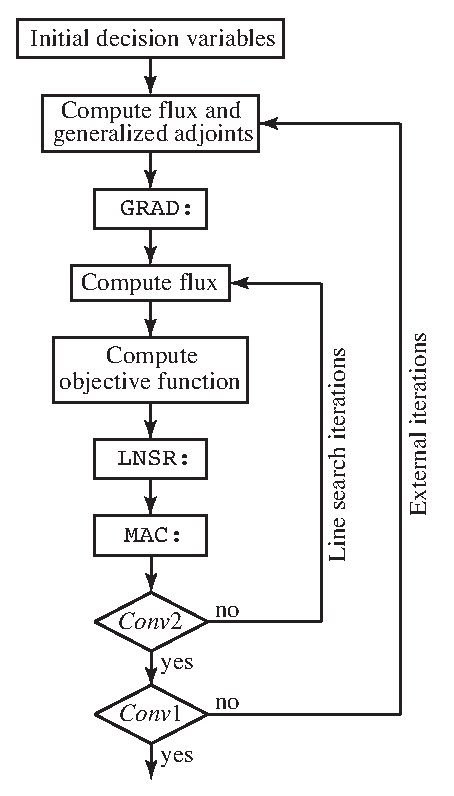
\includegraphics[scale=0.85]{Figures/lnsr.eps} 
\caption{Line search iterations.}\label{fig:fig_lnsr}
\end{center}
\end{figure}

The calling specifications are:

\begin{DataStructure}{Structure \moc{LNSR:}}
\dusa{OPTIM} \moc{:=} \moc{LNSR:} \dusa{OPTIM} \moc{::} \dstr{lnsr\_data}
\end{DataStructure}

\noindent where

\begin{ListeDeDescription}{mmmmmmmm}

\item[\dusa{OPTIM}] \texttt{character*12} name of the \dds{optimize} object ({\tt L\_OPTIMIZE} signature) containing the
optimization informations. Object \dusa{OPTIM} must appear on both LHS and RHS to be able to update the previous values.

\item[\dstr{lnsr\_data}] structure containing the data to the module \texttt{LNSR:} (see Sect.~\ref{sect:lnsr_data}).

\end{ListeDeDescription}
\vskip 0.2cm
\goodbreak

\subsubsection{Data input for module \texttt{LNSR:}}\label{sect:lnsr_data}

\begin{DataStructure}{Structure \moc{lnsr\_data}}
$[$ \moc{EDIT} \dusa{iprint} $]$ \\
$[~\{$ \moc{MAXIMIZE} $|$ \moc{MINIMIZE} $\}~]$ \\
$[$ \moc{OUT-STEP-LIM} \dusa{sr} $]$ \\
$[$ \moc{OUT-STEP-EPS} \dusa{$\epsilon_{ext}$} $]~[$ \moc{INN-STEP-EPS} \dusa{$\epsilon_{inn}$} $]$ \\
\moc{OUT-ITER-MAX} \dusa{maxE} \\
$[$ \moc{OUT-RESTART} \dusa{nstart} $]$ \\
$[~\{$ \moc{SD} $|$ \moc{CG} $|$ \moc{BFGS} $|$ \moc{LBFGS} $[$ \moc{hist\_nr} $]~|$ \moc{NEWT} $\}~]$ \\
$[$ \moc{INN-CONV-TST} {\tt >>} \dusa{$l_{convI}$} {\tt <<}  \moc{OUT-CONV-TST} {\tt >>} \dusa{$l_{convE}$} {\tt <<} $]$ \\
;
\end{DataStructure}

\noindent where
\begin{ListeDeDescription}{mmmmmmmm}

\item[\moc{EDIT}] keyword used to set \dusa{iprint}.

\item[\dusa{iprint}] index used to control the printing in module.

\item[\moc{MAXIMIZE}] keyword used to specify that the optimization problem will be a maximization.

\item[\moc{MINIMIZE}] keyword used to specify that the optimization problem will be a minimization (default).

\item[\moc{OUT-STEP-LIM}] keyword used to set or reset the maximum stepsize for the line search (default value is \dusa{sr} $=1.0$
or the value recovered from \dusa{OPTIM}).

\item[\dusa{sr}] initial radius of the stepsize (real or double precision).

\item[\moc{OUT-STEP-EPS}] keyword used to set the tolerance of outer iteration convergence inside module {\tt LNSR:} (default value
is $1.0 \times 10^{-4}$).

\item[\dusa{$\epsilon_{ext}$}] tolerance value (real or double precision).

\item[\moc{INN-STEP-EPS}] keyword used to set the tolerance used for the line search algorithm (default value
is $1.0 \times 10^{-4}$).

\item[\dusa{$\epsilon_{inn}$}] tolerance value (real or double precision).

\item[\moc{OUT-ITER-MAX}] keyword used to set the maximum number of external iterations.

\item[\dusa{maxE}] maximum number of external iterations.

\item[\moc{OUT-RESTART}] keyword used to set the external iteration restart cycle. A new recursion cycle
is restarted from the conjugate gradient method. By default, no restart is performed.

\item[\dusa{nstart}] number of iterations in one external iteration restart cycle.

\item[\moc{SD}] steepest descent method (default option).

\item[\moc{CG}] conjugate gradient method.

\item[\moc{BFGS}] Broyden-Fletcher-Goldfarb-Shanno method.\cite{recipie}

\item[\moc{LBFGS}] Memory limited Broyden-Fletcher-Goldfarb-Shanno method.\cite{nocedal}

\item[\dusa{hist\_nr}] number of corrections used in the memory limited Broyden-Fletcher-Goldfarb-Shanno method (default value
is 10).

\item[\moc{NEWT}] Newton method for unconstrained optimization.\cite{sph1981}

\item[\moc{INN-CONV-TST}] keyword used to determine if the line search convergence has been reached.

\item[\dusa{$l_{convI}$}] $=1$ means that line search convergence has been reached; $=0$ otherwise.

\item[\moc{OUT-CONV-TST}] keyword used to determine if the external convergence has been reached.

\item[\dusa{$l_{convI}$}] $=1$ means that external convergence has been reached; $=0$ otherwise.

\end{ListeDeDescription}
\clearpage

\vskip 1.0cm
\subsection{The \texttt{FPSPH:} module}

The {\tt FPSPH:} module performs a single fixed-point (aka. Picard) or Newton SPH iteration. This module is intended to be used in
a {\tt REPEAT UNTIL} loop, implemented in CLE-2000 macro-language, where the macro calculation is explicitely called, as depicted
in Figs.~\ref{fig:fig_fpsph} and~\ref{fig:fig_fnewton}.

\vskip 0.2cm

\begin{figure}[h!]
\begin{center}
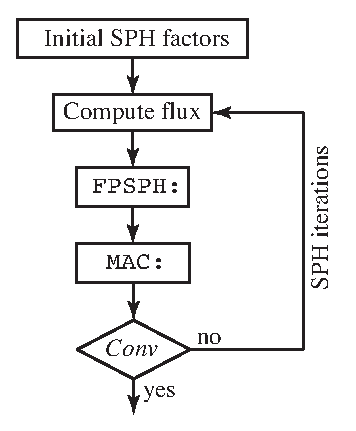
\includegraphics[scale=0.85]{Figures/fpsph.eps} 
\caption{Fixed point SPH iterations.}\label{fig:fig_fpsph}
\end{center}
\end{figure}

\begin{figure}[h!]
\begin{center}
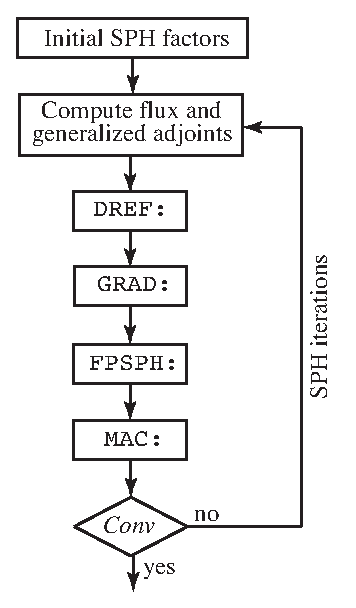
\includegraphics[scale=0.85]{Figures/flow_newton.eps} 
\caption{Newton SPH iterations.}\label{fig:fig_fnewton}
\end{center}
\end{figure}

\clearpage

The calling specifications are:

\begin{DataStructure}{Structure \moc{FPSPH:}}
\dusa{OPTIM} \moc{:=} \moc{FPSPH:} $[$ \dusa{OPTIM} $]$ \dusa{MACROLIB} \dusa{MACROREF} \moc{::} \dstr{fpsph\_data}
\end{DataStructure}

\noindent where

\begin{ListeDeDescription}{mmmmmmmm}

\item[\dusa{OPTIM}] \texttt{character*12} name of the \dds{optimize} object ({\tt L\_OPTIMIZE} signature) containing the
SPH factors. At the first call, object \dusa{OPTIM} must appear on LHS to receive its initial values. On subsequent calls, object
\dusa{OPTIM} must appear on both LHS and RHS to be able to update the previous values.

\item[\dusa{MACROLIB}] \texttt{character*12} name of the read-only extended \dds{macrolib} object ({\tt L\_MACROLIB} signature) containing the
macroscopic cross sections used by the macro-calculation and fluxes produced by the macro-calculation.

\item[\dusa{MACROREF}] \texttt{character*12} name of the read-only extended \dds{macrolib} object ({\tt L\_MACROLIB} signature) containing the
reference macroscopic cross sections and fluxes.

\item[\dstr{fpsph\_data}] structure containing the data to the module \texttt{FPSPH:} (see Sect.~\ref{sect:lnsr_data}).

\end{ListeDeDescription}
\vskip 0.2cm

\subsubsection{Data input for module \texttt{FPSPH:}}\label{sect:lnsr_data}

\begin{DataStructure}{Structure \moc{fpsph\_data}}
$[$ \moc{EDIT} \dusa{iprint} $]$ \\
$[~$\moc{SPH} $\{$ \moc{PN} $|$ \moc{SN} $\}~]$ \\
$[$ \moc{GRPMIN} \dusa{ngr1} $]~[$ \moc{GRPMAX} \dusa{ngr2} $]$\\
$[$ \moc{OUT-STEP-EPS} \dusa{$\epsilon_{ext}$} \\
$[$ \moc{VAR-VAL-MIN} \dusa{varmin} $]~[$ \moc{VAR-VAL-MAX} \dusa{varmax} $]$ \\
$[$ \moc{OUT-CONV-TST} {\tt >>} \dusa{$l_{conv}$} {\tt <<} $[$ {\tt >>} \dusa{$rms_{conv}$} {\tt <<} $]~]$ \\
;
\end{DataStructure}

\noindent where
\begin{ListeDeDescription}{mmmmmmmm}

\item[\moc{EDIT}] keyword used to set \dusa{iprint}.

\item[\dusa{iprint}] index used to control the printing in module.

\item[\moc{PN}] keyword to activate a calculation of heterogeneous SPH factors of diffusion, PN or SPN type.

\item[\moc{SN}] keyword to activate a calculation of heterogeneous SPH factors of PIJ, IC, SN or MOC type.
This is the default option.

\item[\moc{GRPMIN}] keyword used to set the first energy group where SPH correction is applied. By default,
the first energy group index is used.

\item[\dusa{ngr1}] minimum energy group index where SPH correction is applied.

\item[\moc{GRPMAX}] keyword used to set the last energy group where SPH correction is applied. By default,
the total number of energy groups in \dusa{MACROLIB} is used.

\item[\dusa{ngr2}] maximum energy group index where SPH correction is applied.

\item[\moc{OUT-STEP-EPS}] keyword used to set the tolerance of SPH iteration convergence inside module {\tt FPSPH:} (default value
is $1.0 \times 10^{-4}$).

\item[\dusa{$\epsilon_{ext}$}] tolerance value (real or double precision).

\item[\moc{VAR-VAL-MIN}] keyword to specify the minimum values of the SPH factors. These values can also be set in a previous call
to module {\tt GRAD:}.

\item[\dusa{varmin}] single real value used for all SPH factors.

\item[\moc{VAR-VAL-MAX}] keyword to specify the maximum values of the SPH factors. These values can also be set in a previous call
to module {\tt GRAD:}.

\item[\dusa{varmax}] single real value used for all SPH factors.

\item[\moc{OUT-CONV-TST}] keyword used to determine if the SPH convergence has been reached.

\item[\dusa{$l_{conv}$}] $=1$ means that SPH convergence has been reached; $=0$ otherwise.

\item[\dusa{$rms_{conv}$}] RMS error of the converged SPH factors.

\end{ListeDeDescription}
\clearpage


\section{PIN-POWER RECONSTRUCTION MODULES}\label{sect:modesc6}

This section is related to pin-power reconstruction capabilities available in Donjon.
The corresponding theory is explained in \cite{Chambon2014,Fliscounakis2011} 

\subsection{The {\tt NAP:} module}\label{sect:NAPData}

The \moc{NAP:} module supplies the main transport-diffusion equivalence options to DRAGON and DONJON. It can be
used to perform the pin power reconstruction.\cite{Chambon2014,Fliscounakis2011} The calling specifications are:

\begin{DataStructure}{Structure \dstr{NAP:}}
\dusa{COMPO} \moc{:=} \moc{NAP:} \dusa{COMPO} \dusa{TRKNAM} \dusa{FLUNAM} \moc{::} \dstr{descnap1} \\
\dusa{MAP} \moc{:=} \moc{NAP:} \dusa{MAP} \dusa{TRKNAM} \dusa{FLUNAM} \dusa{MATEX} \dusa{MACRES} \moc{::} \dstr{descnap2} \\
\dusa{GEONEW} \moc{:=} \moc{NAP:} \dusa{GEOOLD} \dusa{COMPO} \moc{::} \dstr{descnap3} \\
\end{DataStructure}

\noindent
where
\begin{ListeDeDescription}{mmmmmmmm}

\item[\dusa{COMPO}] {\tt character*12} name of the \dds{multicompo} data
structure ({\tt L\_COMPO} signature) where the detailed subregion properties will be stored.

\item[\dusa{TRKNAM}] {\tt character*12} name of the read-only \dds{tracking} data
structure ({\tt L\_TRACK} signature) containing the tracking. 

\item[\dusa{FLUNAM}] {\tt character*12} name of the read-only \dds{fluxunk} data
structure ({\tt L\_FLUX} signature) containing a transport solution.

\item[\dusa{MAP}] {\tt character*12} name of the \dds{map} data
structure ({\tt L\_MAP} signature) containing fuel regions description, global and
local parameter information (burnup, fuel/coolant temperatures, coolant density, etc). A previous call to the \moc{FLPOW:} module is highly recommended prior to the pin-power reconstruction to normalize the flux and compute the assembly power. If not, the pin-power reconstruction  will be normalized using the whole core power instead of a normalization for each assembly.
Keyword \moc{PPR} is expected in \dstr{descnap2}.

\item[\dusa{MATEX}] {\tt character*12} name of the read-only \dds{matex} data
structure ({\tt L\_MATEX} signature). The object corresponds to the heterogeneously splited geometry. Keyword \moc{PPR} is expected in \dstr{descnap2}.

\item[\dusa{MACRES}] {\tt character*12} name of the read-only \dds{macrolib} data
structure ({\tt L\_MACROLIB} signature) containing a cross section for the fuel. The \dds{macrolib} data
structure must have been created with a \dds{multicompo} data structure with pin level properties (transport flux, H-factor, infinite domain diffusion flux). Keyword \moc{PPR} is expected in \dstr{descnap2}.

\item[\dusa{GEONEW}] {\tt character*12} name of the created \dds{geometry} data
structure ({\tt L\_GEOM} signature) containing the detailed core geometry definition at heterogeneous assembly level.

\item[\dusa{GEOOLD}] {\tt character*12} name of the read-only \dds{geometry} data
structure ({\tt L\_GEOM} signature) containing the core geometry definition with homogeneous assembly (only 1 mesh per assembly mandatory).

\item[\dstr{descnap1}] structure containing the input data to this module to compute additional properties for subregions
(see \Sect{descnap1}).

\item[\dstr{descnap2}] structure containing the input data to this module to perform pin power reconstruction
(see \Sect{descnap2}).

\item[\dstr{descnap3}] structure containing the input data to this module to automatically define the core geometry with heterogeneous assembly
(see \Sect{descnap3}).

\end{ListeDeDescription}

\subsubsection{Additional properties calculations}\label{sect:descnap1}

\begin{DataStructure}{Structure \dstr{descnap1}}
$[$ \moc{EDIT} \dusa{iprint} $]$ \\
\moc{PROJECTION}\\
 \moc{STEP} \dusa{namedir} \\
$[$ \moc{IFX} \dusa{ifx} $]$ \\
$\{$ $[[$ \moc{SET} \dusa{pname} \dusa{pvalue} $]]$ $\}$ \\
;
\end{DataStructure}

\noindent where

\begin{ListeDeDescription}{mmmmmmmm}

\item[\moc{EDIT}] keyword used to modify the print level \dusa{iprint}.

\item[\dusa{iprint}] integer index used to control  the printing in module {\tt NAP:}.
=0 for no print; =1 for minimum printing (default value); larger values of \dusa{iprint}
will produce increasing amounts of output.

\item[\moc{PROJECTION}] keyword to specify that additional properties for subregions will be computed and stored in the \dds{multicompo} data-structure \dusa{COMPO}.

\item[\moc{STEP}] keyword to specify \dusa{namedir}. 

\item[\dusa{namedir}] name of the directory containing the homogenized cross sections (homogeneous or heterogeneous). 

\item[\moc{IFX}] keyword to specify \dusa{ifx}. 

\item[\dusa{ifx}] number used to create the name of the flux record representing $\psi_{m,p}^{d,\infty}$. This flux represents the results of calculation in an infinite domain computed in diffusion with cross sections homogenized either homogeneously or heterogeneously. One record is associated with each type of homogenization when the \dds{multicompo} is created. Thus \dds{multicompo} can be "enriched" up to 5 times, each time using a different homogenization of the assembly at the end of the transport calculations. The following format is used for the flux record name (\verb+RECNAME+): \\
\verb+WRITE(RECNAME,'5HFINF_,I3.3') IFX+\\
Thus, for example for \dusa{ifx}=2, \verb+RECNAME+ would be \verb+FINF_002+.

\item[\moc{SET}] keyword to specify assembly calculations at which $\psi_{m,p}^{d,\infty}$ have been calculated. Repeated as many times as there are parameters in the \dds{multicompo}.

\item[\dusa{pname}] name of the parameter in the \dds{multicompo}. 

\item[\dusa{pvalue}] value of the parameter in the \dds{multicompo}. 

\end{ListeDeDescription}

Note that in the case of heterogeneously homogenized assembly, the pin-wise projected diffusion flux is stored in mixture 1.

\subsubsection{Pin power reconstruction}\label{sect:descnap2}

\begin{DataStructure}{Structure \dstr{descnap2}}
$[$ \moc{EDIT} \dusa{iprint} $]$ \\
\moc{PPR}\\
\moc{NZASS} \dusa{nzass}  \\ 
\moc{METH}  %$\{$  \\
     \moc{GPPR} \dusa{ifx} %$\}$
\\
$[$ \moc{POWER} \dusa{pow} $]$ \\
;
\end{DataStructure}

\noindent where

\begin{ListeDeDescription}{mmmmmmmm}

\item[\moc{EDIT}] keyword used to modify the print level \dusa{iprint}.

\item[\dusa{iprint}] index used to control the printing of this module. The
\dusa{iprint} parameter is important for adjusting the amount of data that is
printed by this calculation step:

\begin{itemize}

\item \dusa{iprint}=0 results in no output;

\item \dusa{iprint}=1 ...

\end{itemize}

\item[\moc{PPR}] keyword to perform pin power reconstruction and stored results in the \dds{map} data-structure \dusa{MAP}.

\item[\moc{NZASS}] keyword to specify \dusa{nzass}. 

\item[\dusa{nzass}] number of mesh in Z direction along assemblies. 

\item[\moc{METH}] keyword to select the type of methodology used for pin power reconstruction.

\item[\moc{GPPR}] keyword to select the generalized pin power reconstruction from an heterogeneous assembly definition (several mixtures per assembly). Note that if there is only one mixture (homogeneous assembly) this method is actually the regular pin power reconstruction.

\item[\dusa{ifx}] number used to create the named of the flux record representing $\psi_{m,p}^{d,\infty}$. See Sect. \ref{sect:descnap1} for more details.

\item[\moc{POWER}] keyword used to normalize the flux. If this keyword is not used, the flux directly computed by the \moc{FLUD:} is used to perform the pin-power reconstruction,  then normalization has to be performed either previously by the \moc{FLPOW:} module  or by the user independently. 

\item[\dusa{pow}] power used to normalize the flux (MW). 

\end{ListeDeDescription}

\clearpage

\subsubsection{Heterogeneous assembly geometry definition}\label{sect:descnap3}

\begin{DataStructure}{Structure \dstr{descnap3}}
$[$ \moc{EDIT} \dusa{iprint} $]$ \\
\moc{DIRGEO} \dusa{namedir} $[$ \moc{MACGEO} $]$  \\
\moc{MIXASS} \dusa{nmix} (\dusa{imix}(i), i=1,\dusa{nmix})  \\
$[$ \moc{SLPITX-ASS} (\dusa{ispx}(i), i=1,\dusa{nxass}) $]$ \\
$[$ \moc{SLPITY-ASS} (\dusa{ispy}(i), i=1,\dusa{nyass}) $]$ \\
$[$ \moc{MAX-MIX-GEO} \dusa{nmxgeo} $]$ \\
;
\end{DataStructure}

\noindent where

\begin{ListeDeDescription}{mmmmmmmm}

\item[\moc{EDIT}] keyword used to modify the print level \dusa{iprint}.

\item[\dusa{iprint}] index used to control the printing of this module. The
\dusa{iprint} parameter is important for adjusting the amount of data that is
printed by this calculation step:

\begin{itemize}

\item \dusa{iprint}=0 results in no output;

\item \dusa{iprint}=1 ...

\end{itemize}

\item[\moc{DIRGEO}] keyword to specify \dusa{namedir}. 

\item[\dusa{namedir}] name of the directory containing the heterogeneously or homogeneously homogenized cross sections. 

\item[\moc{MACGEO}] keyword to specify that the macro-geometry stored in the \dusa{GFF} record of the macrolib will be used instead of the macro-geometry of the  heterogeneously or homogeneously homogenized cross sections. Usually this other macro-geometry of the assembly corresponds to the pin-by-pin geometry. Note that another multicompo with all pin-wise properties is needed to be able to use the automatically generated geometry. 

\item[\moc{MIXASS}] keyword to specify mixtures corresponding to assembly in the coarse geometry. 

\item[\dusa{nmix}] number of type of assembly. 

\item[\dusa{imix}] mixture number of the assemblies.

\item[\moc{SLPITX-ASS}] keyword to specify the mesh splitting at assembly level. 

\item[\dusa{ispx}] split along x-direction for each mesh of the heterogeneous assembly. 

\item[\dusa{nxass}] number of mesh of the heterogeneous assembly along x-direction. 

\item[\moc{SLPITY-ASS}] keyword to specify the mesh splitting at assembly level. 

\item[\dusa{ispy}] split along y-direction for each mesh of the heterogeneous assembly. 

\item[\dusa{nyass}] number of mesh of the heterogeneous assembly along y-direction. 

\item[\moc{MAX-MIX-GEO}] keyword to specify the number of mixtures in the original core geometry (i.e. before the core geometry is splited by the \moc{NAP:} module). This keyword is mandatory if there is a reflector in the geometry otherwise the numbers for fuel mixtures will not match between the split core geometry (\dds{geometry}) and the split fuel geometry (\dds{geometry} embedded in \dds{map}).

\item[\dusa{nmxgeo}] number of mixtures in the original core geometry. 

\end{ListeDeDescription}

{\bf Note: The included geometry in the \dusa{COMPO} has to be unfolded, even if the transport calculations are done on a 1/8th assembly. Moreover no split can be defined in the geometry, one mesh ONLY per heterogeneous mixture  is mandatory.} 

\eject


